% !TeX program = xelatex
\AddToHook{package/projlib-language/before}{\RequirePackage{fvextra}}
\documentclass[11pt,a4paper,oneside,plain,CN,colored-proof=false,
  load-custom-latin-font-file=pku-font-latin.tex,
  load-custom-math-font-file=pku-font-math.tex,
  load-custom-cjk-font-file=pku-font-cjk.tex]{einfart}
% 学习总笔记：公共配置见 ../common/zbstyle.tex。
\newcommand{\PKUDocumentType}{notes}
\newcommand{\PKUCodePalette}{ide}
\newcommand{\PKUShortTitle}{应用线性回归}
\newcommand{\PKUSubtitle}{公共卫生统计 · 学习总笔记}
\newcommand{\PKUVersion}{2.0}

\usepackage{pku-notes}
% 公卫统计 · Einfart/plain 学习总笔记兼容层
% 视觉设置集中于本文件和 pku-notes.sty；原章节、题号、标签保持不变。
\usepackage{multirow,calc,tikz,pgfplots,placeins,pdflscape,microtype}
\usetikzlibrary{arrows.meta,positioning,calc,patterns,decorations.pathreplacing,shapes.geometric}
\pgfplotsset{compat=1.18}
\colorlet{PKUInk}{black}
\colorlet{Ink}{black}
\colorlet{Muted}{PKUMuted}
\colorlet{Primary}{PKURed}
\colorlet{Accent}{PKURed}
\colorlet{Rule}{black!22}
\colorlet{Paper}{PKUTint}
\colorlet{CodeBackground}{PKUCodeBg}
\colorlet{CodeRule}{black!22}
\colorlet{NavyBlue}{PKURed}
\colorlet{DarkRed}{PKURed}
\colorlet{ForestGreen}{black!65}
\colorlet{BoxGray}{black!3}
\colorlet{DefBlue}{PKURed!4}
\colorlet{ThmGold}{PKURed!3}
\colorlet{ExGreen}{black!3}
\colorlet{RemPurple}{black!3}
% 代码语义配色独立于装饰色。
\colorlet{CodeKeyword}{PKUCodePurple}
\colorlet{CodeFunction}{PKUCodeBlue}
\colorlet{CodeString}{PKUCodeString}
\colorlet{CodeComment}{PKUCodeGreen}
\definecolor{CodeConstant}{HTML}{805600}
\providecommand{\bm}[1]{\symbf{#1}}
\setlength{\emergencystretch}{3em}
\clubpenalty=10000\widowpenalty=10000\displaywidowpenalty=10000
\allowdisplaybreaks[2]
\setcounter{MaxMatrixCols}{14}
\setlength{\tabcolsep}{5pt}
\renewcommand{\arraystretch}{1.18}
\setlength{\heavyrulewidth}{.7pt}
\setlength{\lightrulewidth}{.35pt}
\setlength{\cmidrulewidth}{.3pt}
\captionsetup{font={small,pkublack},labelfont={bf,sf,pkublack},
  textfont={pkublack},labelsep=quad,skip=6pt,hypcap=false}
% Einfart 原生为 article。用 titlesec 增加 chapter 层，保留书稿结构。
\makeatletter
\def\ttll@part{-1}
\makeatother
\titleclass{\chapter}{top}[\part]
\newcounter{chapter}
\renewcommand{\thechapter}{\arabic{chapter}}
\counterwithin{section}{chapter}
\counterwithin{equation}{chapter}
\counterwithin{figure}{chapter}
\counterwithin{table}{chapter}
\providecommand{\theHchapter}{\arabic{chapter}}
\renewcommand{\thesection}{\thechapter.\arabic{section}}
\renewcommand{\chaptermark}[1]{\markboth{第\thechapter 章\quad #1}{}}
\titleformat{\chapter}[display]
  {\raggedright\sffamily\bfseries\color{black}}
  {\large\bfseries\color{black}第\,\thechapter\,章}{7pt}
  {\fontsize{23}{31}\selectfont\bfseries\color{black}#1}
  [\vspace{8pt}{\color{PKURed}\rule{\linewidth}{.7pt}}]
\titleformat{name=\chapter,numberless}[display]
  {\raggedright\sffamily\bfseries\color{black}}{}{0pt}
  {\fontsize{23}{31}\selectfont\bfseries\color{black}#1}
  [\phantomsection\vspace{8pt}{\color{PKURed}\rule{\linewidth}{.7pt}}]
\titlespacing*{\chapter}{0pt}{0pt}{22pt}
\titleformat{\section}
  {\sffamily\bfseries\Large\color{black}}{\thesection}{.7em}{#1}
\titleformat{\subsection}
  {\sffamily\bfseries\large\color{black}}{\thesubsection}{.65em}{#1}
\titleformat{\subsubsection}
  {\sffamily\bfseries\normalsize\color{black}}{\thesubsubsection}{.6em}{#1}
\setcounter{secnumdepth}{2}\setcounter{tocdepth}{1}
\pretocmd{\section}{\ifinner\else\Needspace{6\baselineskip}\fi}{}{}
\pretocmd{\subsection}{\ifinner\else\Needspace{4\baselineskip}\fi}{}{}
\newcommand{\frontmatter}{\clearpage\pagenumbering{Roman}}
\newcommand{\mainmatter}{\clearpage\pagenumbering{arabic}\setcounter{chapter}{0}}
\titlecontents{chapter}[3.2em]
  {\addvspace{.55\baselineskip}\PKUTOCFont}
  {\contentslabel[第\thecontentslabel 章]{3.2em}}{\hspace*{-3.2em}}
  {\titlerule*[.7em]{.}\contentspage}
\titlecontents{section}[5.4em]
  {\addvspace{.12\baselineskip}\small\PKUTOCFont}
  {\contentslabel{3em}}{\hspace*{-3em}}
  {\titlerule*[.7em]{.}\contentspage}
\makeatletter
\providecommand{\@chapapp}{章}
\renewcommand{\@pnumwidth}{2.5em}
\renewcommand{\@tocrmarg}{3.5em}
\def\toclevel@chapter{0}
\newcommand{\ZBTableOfContents}{\clearpage\chapter*{目录}%
  \markboth{目录}{}\begingroup\hypersetup{linkcolor=black}%
  \setlength{\parskip}{0pt}\@starttoc{toc}\endgroup}
\makeatother
% 页眉页脚：低对比辅助信息，页码常规字重。
\newcommand{\BookShortTitle}{\PKUShortTitle}
\newcommand{\ZBPageFurniture}{\fancyhf{}%
  \fancyhead[L]{\footnotesize\normalfont\sffamily\color{Muted}\nouppercase{\leftmark}}%
  \fancyhead[R]{\footnotesize\normalfont\sffamily\color{Muted}\BookShortTitle}%
  \fancyfoot[C]{\small\normalfont\sffamily\color{Muted}\thepage}%
  \renewcommand{\headrulewidth}{.3pt}\renewcommand{\footrulewidth}{0pt}}
\fancypagestyle{pku}{\ZBPageFurniture}
\fancypagestyle{plain}{\ZBPageFurniture}
\hypersetup{linkcolor=PKURed,urlcolor=PKURed,citecolor=PKURed}
\pdfstringdefDisableCommands{\def\color#1{}\def\sffamily{}\def\bfseries{}%
  \def\enspace{ }\def\quad{ }\def\texorpdfstring#1#2{#2}}
% 保留原正文环境，标题均在字体选择后显式设为黑色。
\tcbset{zbbase/.style={enhanced jigsaw,breakable,sharp corners,frame hidden,
  boxrule=0pt,before skip=9pt plus 2pt,after skip=9pt plus 2pt,pad at break*=1.5mm}}
\newtcolorbox{zbderive}[1]{zbbase,colback=PKURed!3,
  borderline west={1.5pt}{0pt}{PKURed},left=11pt,right=9pt,top=7pt,bottom=7pt,
  before upper={\setlength{\parskip}{3pt}{\sffamily\bfseries\color{black}#1}\par\smallskip}}
\newtcolorbox{zbnote}[1][批注]{zbbase,colback=white,
  borderline west={.8pt}{0pt}{black!35},left=9pt,right=2pt,top=2pt,bottom=2pt,
  fontupper=\small\color{Muted},
  before upper={{\sffamily\bfseries\color{black}#1}\enspace}}
\newtcolorbox{zbcheck}[1][说明]{zbbase,colback=PKURed!2,
  borderline west={1.2pt}{0pt}{PKURed},left=10pt,right=8pt,top=5pt,bottom=5pt,
  fontupper=\small\color{black},
  before upper={{\sffamily\bfseries\color{black}#1}\enspace}}
\newtcolorbox{keyidea}[1][]{zbbase,colback=PKURed!2,
  borderline west={1.3pt}{0pt}{PKURed},left=11pt,right=9pt,top=6pt,bottom=6pt,
  before upper={\ifx\relax#1\relax\else{\sffamily\bfseries\color{black}#1}\par\smallskip\fi}}
\newcommand{\dpart}[1]{\par\noindent{\sffamily\bfseries\color{black}#1}\quad\ignorespaces}
\let\question\relax
\let\answer\relax
\newcommand{\question}[1]{\par\Needspace{3\baselineskip}\smallskip\noindent
  {\sffamily\bfseries\color{black}问}\quad #1\par\smallskip}
\newcommand{\answer}[1]{\par\smallskip\noindent
  {\sffamily\bfseries\color{black}答}\quad #1\par\smallskip}
\newlist{choices}{enumerate}{1}
\setlist[choices]{label=\Alph*.,leftmargin=2.2em,itemsep=4pt,topsep=4pt,parsep=0pt,labelsep=.6em}
\newcounter{zbquestion}
\newcommand{\exsetno}{0}
\renewcommand{\thezbquestion}{\exsetno.\arabic{zbquestion}}
\renewcommand{\theHzbquestion}{\exsetno.\arabic{zbquestion}}
\newcommand{\ZBQuestion}[2]{\par\addvspace{12pt}\ifinner\else\Needspace{5\baselineskip}\fi
  \refstepcounter{zbquestion}\label{q:#1}\noindent
  {\sffamily\bfseries\color{black}题\thezbquestion}\quad
  {\sffamily\bfseries\color{black}#2}\par\nobreak\smallskip}
% unicode-math 在文档开始时把 Question 定义为双问号数学符号。
% 在所有字体/符号初始化完成后恢复原笔记的题面命令。
\AddToHook{begindocument/end}{\let\Question\ZBQuestion}
\newcommand{\Answer}[2]{\par\addvspace{12pt}\ifinner\else\Needspace{5\baselineskip}\fi\noindent
  {\sffamily\bfseries\color{black}解析\enspace 题\ref*{q:#1}}\quad
  {\sffamily\bfseries\color{black}#2}%
  \hfill{\footnotesize\sffamily\hyperref[q:#1]{\color{Muted}返回题目}}%
  \par\nobreak\smallskip\label{a:#1}}
\newcommand{\worklines}[1]{\par\smallskip{\color{Rule}\vbox{\offinterlineskip
  \foreach \n in {1,...,#1}{\vskip7.5mm\hrule height.3pt width\linewidth}}}\par\vspace{6pt}}
\DefineVerbatimEnvironment{verbatim}{Verbatim}{breaklines,fontsize=\small,formatcom=\xeCJKVerbAddon}
\DefineVerbatimEnvironment{Highlighting}{Verbatim}{breaklines,commandchars=\\\{\},fontsize=\small,formatcom=\xeCJKVerbAddon}
\providecommand{\tightlist}{\setlength{\itemsep}{0pt}\setlength{\parskip}{0pt}}
\providecommand{\pandocbounded}[1]{#1}
\providecommand{\passthrough}[1]{#1}
\AtBeginEnvironment{longtable}{\small\setlength{\tabcolsep}{4pt}\renewcommand{\arraystretch}{1.22}}
\setlength{\LTpre}{6pt}\setlength{\LTpost}{6pt}
\newcommand{\ExerciseNumber}[1]{\renewcommand{\exsetno}{#1}}
\newcommand{\ExerciseChapter}[1]{\clearpage\setcounter{zbquestion}{0}%
  \setcounter{secnumdepth}{0}\thispagestyle{plain}\phantomsection
  \addcontentsline{toc}{section}{\protect\numberline{}习题与解析\enspace #1}%
  \addtocontents{toc}{\protect\setcounter{tocdepth}{0}}%
  \markboth{第\exsetno 章\quad 习题与解析}{}%
  {\raggedright\sffamily\bfseries\color{black}%
   {\large\bfseries\color{black}第\,\exsetno\,章\enspace 习题与解析}\par\vspace{7pt}%
   {\fontsize{23}{31}\selectfont\bfseries\color{black}#1}\par\vspace{8pt}%
   {\color{PKURed}\rule{\linewidth}{.7pt}}\par}\vspace{22pt}%
  \pdfbookmark[1]{习题与解析：#1}{ex:\exsetno}}
\newcommand{\EndExercises}{\addtocontents{toc}{\protect\setcounter{tocdepth}{1}}\setcounter{secnumdepth}{2}}
% 简约封面：课程名、英文名、居中校徽、学习网站与日期。
\newcommand{\MakeCover}[2]{%
  \begin{titlepage}\thispagestyle{empty}\hypersetup{pageanchor=false}%
  \begin{tikzpicture}[remember picture,overlay]
    \node[align=center,text width=.88\paperwidth]
      at ([yshift=60mm]current page.center)
      {{\sffamily\fontsize{32}{43}\selectfont\bfseries\color{black}#1}};
    \node[align=center,text width=.88\paperwidth]
      at ([yshift=42mm]current page.center)
      {{\sffamily\fontsize{14}{20}\selectfont\color{Muted}#2}};
    \node at (current page.center)
      {
\includegraphics[width=44mm]{../common/pku-emblem.jpg}};
    \node[align=center,text width=.88\paperwidth]
      at ([yshift=39mm]current page.south)
      {{\small\sffamily\color{Muted}学习网站：\url{https://fxt-gw-pb.github.io/public-health-statistics-notes/}}};
    \node at ([yshift=24mm]current page.south)
      {{\small\color{Muted}2026年10月}};
  \end{tikzpicture}%
  \null\end{titlepage}\hypersetup{pageanchor=true}}
% ---- 2026-10-06 润色补充：讲解框、运行结果、章末复习 ----
\DefineVerbatimEnvironment{routput}{Verbatim}{breaklines,breakanywhere,
  fontsize=\fontsize{8.6}{11.2}\selectfont,formatcom=\color{black!80}\xeCJKVerbAddon,
  frame=leftline,framerule=.8pt,rulecolor=\color{black!28},framesep=7pt,xleftmargin=12pt}
\newtcolorbox{sikao}[1][说明]{zbbase,colback=black!2.5,
  borderline west={1.2pt}{0pt}{black!50},left=10pt,right=8pt,top=6pt,bottom=6pt,
  before upper={\setlength{\parskip}{4pt}{\sffamily\bfseries\color{black}#1}\par\smallskip}}
\newtcolorbox{fuxi}[1][本章要点]{zbbase,colback=PKURed!2,
  borderline west={1.5pt}{0pt}{PKURed},left=11pt,right=9pt,top=7pt,bottom=7pt,
  before upper={\setlength{\parskip}{3pt}{\sffamily\bfseries\color{black}#1}\par\smallskip}}

% 应用线性回归：讲解部分所用宏（按总笔记版式重新定义）
\colorlet{TextInk}{Ink}
\colorlet{NoteGray}{Muted}
\colorlet{RuleGray}{Rule}
\colorlet{ChartForest}{PKURed}
\colorlet{ChartBrick}{black!65}
\colorlet{ChartOchre}{black!40}
\colorlet{CodePaper}{CodeBackground}
\pgfplotsset{every axis/.append style={font=\small,axis line style={draw=Ink!70,line width=.55pt},
  tick style={draw=Ink!60,line width=.45pt},tick align=outside,clip marker paths=false,
  tick label style={font=\footnotesize,color=Ink},label style={font=\small,color=Ink},
  title style={font=\small\bfseries\sffamily,color=Ink},grid=major,major grid style={draw=Ink!12,line width=.25pt},
  legend style={draw=none,fill=white,fill opacity=.96,text opacity=1,font=\footnotesize,inner sep=3pt,row sep=2pt},
  legend cell align=left,every axis plot/.append style={line width=.8pt},every mark/.append style={line width=.65pt}}}
\lstdefinelanguage{CourseR}{sensitive=true,alsoletter={._0123456789},
  morekeywords=[1]{if,else,repeat,while,function,for,in,next,break,TRUE,FALSE,NULL,NA,NaN,Inf},
  morekeywords=[2]{AIC,aggregate,anova,apply,as.data.frame,as.factor,c,cbind,contr.poly,cor,cov,data.frame,det,diag,ezANOVA,library,list,lm,log,matrix,mauchly.test,mean,model.matrix,pchisq,plot,print,regsubsets,rep,resid,solve,step,sum,summary,t,which.max},
  morecomment=[l]\#,morestring=[b]",morestring=[b]'}
\lstdefinestyle{courseR}{language=CourseR,basicstyle=\ttfamily\fontsize{9.3}{12.8}\selectfont\color{Ink},
  keywordstyle=[1]\color{CodeKeyword}\bfseries,keywordstyle=[2]\color{CodeFunction}\bfseries,
  commentstyle=\color{CodeComment}\itshape,stringstyle=\color{CodeString},
  numbers=left,numberstyle=\ttfamily\fontsize{7.3}{10}\selectfont\color{Muted!80},numbersep=9pt,
  backgroundcolor=\color{CodeBackground},frame=single,rulecolor=\color{CodeRule},framerule=.4pt,framesep=6pt,
  xleftmargin=25pt,xrightmargin=7pt,aboveskip=10pt,belowskip=10pt,breaklines=true,breakatwhitespace=false,
  breakindent=14pt,columns=fullflexible,keepspaces=true,showstringspaces=false,tabsize=2,upquote=true,
  literate={<-}{{{\color{Muted}\textless-}}}2 {\%*\%}{{{\color{Muted}\%*\%}}}3}
\lstnewenvironment{rcode}{\lstset{style=courseR}}{}
\newcommand{\ann}[1]{\begin{zbnote}#1\end{zbnote}}
\newenvironment{derivation}[1]{\begin{zbderive}{#1}}{\end{zbderive}}
\DeclareMathOperator{\tr}{tr}
\let\Var\relax
\DeclareMathOperator{\Var}{Var}
\let\Cov\relax
\DeclareMathOperator{\Cov}{Cov}
\DeclareMathOperator{\rank}{rank}
\newcommand{\SSq}[1]{\mathrm{SS}_{\text{#1}}}
\newcommand{\ms}[1]{\mathrm{MS}_{\text{#1}}}
\newcommand{\code}[1]{\texttt{\detokenize{#1}}}
\newcommand{\tbltitle}[1]{\par\smallskip\begin{center}\small\sffamily\bfseries\color{black}#1\end{center}\vspace{-5pt}}
\newcommand{\figtitle}[1]{\par\vspace{3pt}{\small\sffamily\color{Muted}\centering #1\par}\smallskip}

\renewcommand{\BookShortTitle}{应用线性回归}
\hypersetup{pdftitle={应用线性回归·学习总笔记},pdfauthor={},pdfsubject={公共卫生统计}}
\begin{document}
\MakeCover{应用线性回归}{Applied Linear Regression}
\frontmatter
\ZBTableOfContents
\mainmatter
\chapter{矩阵知识简介}
回归分析中的参数估计、方差分析、杠杆值与共线性诊断均以矩阵形式表述，本章先整理后续各章所需的矩阵知识。本章将数据矩阵视为一张数据表及其运算规则：每一行对应一个观察对象，每一列对应一个变量。

本章的重点有以下三项：
\begin{itemize}
\item 均数向量、协方差阵与相关阵分别描述数据的集中位置、变量间的共同变化，以及消除量纲后的共同变化；
\item 线性组合的方差$a^\top\Sigma a$。回归系数的标准误、预测区间与方差分析的期望均方均由该式导出；
\item 特征值与特征向量的统计含义：特征向量表示一个方向，特征值为数据在该方向上的方差。第3章的共线性诊断与多元分析中的主成分分析均以此为基础。
\end{itemize}
\section{矩阵和向量}
\par\noindent\begin{minipage}{\linewidth}
\tbltitle{例1.1\quad 某地12名16岁中学生的身高、体重、胸围资料}
\begin{center}\small
\begin{tabular}{rrrr}
\toprule 编号 & 身高（cm，$x_1$） & 体重（kg，$x_2$） & 胸围（cm，$x_3$）\\\midrule
1&171.0&58.5&81.0\\2&175.0&65.0&87.0\\3&159.0&38.0&71.0\\
4&155.3&45.0&74.0\\5&152.0&35.0&63.0\\6&158.3&44.5&75.0\\
7&154.8&44.5&74.0\\8&164.0&51.0&72.0\\9&165.2&55.0&79.0\\
10&164.5&46.0&71.0\\11&159.1&48.0&72.5\\12&164.2&46.5&73.0\\\bottomrule
\end{tabular}\end{center}
\end{minipage}\par\medskip

36个元素$x_{ij}$组成维度是12行3列的矩阵$X$，其中每列元素组成一个向量。
\par\noindent\begin{rcode}
x1 <- c(171,175,159,155.3,152,158.3,154.8,164,165.2,164.5,159.1,164.2)
x2 <- c(58.5,65,38,45,35,44.5,44.5,51,55,46,48,46.5)
x3 <- c(81,87,71,74,63,75,74,72,79,71,72.5,73)
X <- cbind(x1,x2,x3)
\end{rcode}\par\smallskip
\ann{$12\times3$的矩阵。}
以下各节的数值可由下列命令一并求得，其结果列于此处，供阅读各节公式时对照。
\par\noindent\begin{rcode}
colMeans(X)                       # 均数向量，等价于 apply(X,2,mean)
S <- cov(X); round(S,3)           # 样本协方差阵，分母 n-1
L <- crossprod(scale(X,scale=FALSE))  # 离差阵：中心化后的 X'X
all.equal(L, 11*S)                # 验证 L=(n-1)S
round(cor(X),4)                   # 样本相关阵
\end{rcode}
\begin{routput}
       x1        x2        x3 
161.86667  48.08333  74.37500 
       x1     x2     x3
x1 45.722 50.362 32.232
x2 50.362 69.629 45.466
x3 32.232 45.466 35.324
[1] TRUE
       x1     x2     x3
x1 1.0000 0.8926 0.8020
x2 0.8926 1.0000 0.9168
x3 0.8020 0.9168 1.0000
\end{routput}
\subsection{均数向量}
用均数向量反映资料的平均水平：总体均数向量记为$\mu$（参数），样本均数向量记为$\bar X$（由样本算得的估计值）。均数向量默认是列向量，有时用行向量表示；本书统一用$\bar X^\top$表示转置（transpose），其他资料中的$\bar X'$与$\bar X^T$同义。
\[
\mu=\begin{bmatrix}\mu_1\\\mu_2\\\mu_3\end{bmatrix},\qquad
\bar X=\begin{bmatrix}\bar x_1\\\bar x_2\\\bar x_3\end{bmatrix},\qquad
\bar X^\top=\begin{bmatrix}\bar x_1&\bar x_2&\bar x_3\end{bmatrix}.
\]
\[
\code{apply(X,2,mean)}\ \longrightarrow\
\bar X^\top=(161.86667\quad48.08333\quad74.37500).
\]
\ann{按列求平均。}
\subsection{协方差阵}
方差-协方差矩阵（variance-covariance matrix）简称协方差阵，反映$p$个变量间的线性共变关系。它是方阵和对称矩阵，有时只给出右上半或左下半（上三角或下三角阵）。须区分两类对象：
\begin{itemize}
\item 总体协方差阵$\Sigma$：$\sigma_{ij}=\Cov(X_i,X_j)=E[(X_i-\mu_i)(X_j-\mu_j)]$，$\sigma_{ii}$为第$i$个变量的总体方差，是未知参数。
\item 样本协方差阵$S$：$s_{ij}=l_{ij}/(n-1)$，由样本计算，是$\Sigma$的无偏估计。命令\code{cov(X)}给出的是$S$。
\end{itemize}
\[
\Sigma=\begin{bmatrix}\sigma_{11}&\sigma_{12}&\sigma_{13}\\
\sigma_{21}&\sigma_{22}&\sigma_{23}\\\sigma_{31}&\sigma_{32}&\sigma_{33}\end{bmatrix},
\qquad S=\begin{bmatrix}s_{11}&s_{12}&s_{13}\\s_{21}&s_{22}&s_{23}\\s_{31}&s_{32}&s_{33}\end{bmatrix}.
\]
对例1.1，
\[
\code{cov(X)}\ \longrightarrow\
S=\begin{bmatrix}45.722&50.362&32.232\\50.362&69.629&45.466\\32.232&45.466&35.324\end{bmatrix}.
\]
\begin{sikao}[协方差数值的解释]
$s_{12}=50.362>0$表示身高高于平均水平的学生，其体重也倾向于高于平均水平。协方差的数值大小依赖于测量单位：$s_{12}$的单位为cm$\cdot$kg，若身高改以米为单位记录，该值缩小为原来的1/100，而变量间的关系并未改变。因此，协方差的符号可以解释，其绝对大小不宜直接用于判断关联强度。

比较关联强度时需消除量纲，即计算相关系数：
\[
r_{12}=\frac{s_{12}}{\sqrt{s_{11}s_{22}}}=\frac{50.362}{\sqrt{45.722\times69.629}}=0.8926 .
\]
第2章的标准化偏回归系数，以及多元分析中基于协方差阵或相关阵提取主成分的选择，所涉及的都是同一问题：各变量单位不同时，应根据分析目的决定是否消除量纲。
\end{sikao}
\subsection{离均差平方和与离均差积和矩阵}
简称离差阵，用$L$表示，$L=(n-1)S$。
\[
l_{ii}=\sum_{k=1}^{n}(x_{ki}-\bar x_i)^2,\qquad
l_{ij}=\sum_{k=1}^{n}(x_{ki}-\bar x_i)(x_{kj}-\bar x_j),
\quad i,j=1,2,3,\quad i\ne j.
\]
\[
L=\begin{bmatrix}l_{11}&l_{12}&l_{13}\\l_{21}&l_{22}&l_{23}\\l_{31}&l_{32}&l_{33}\end{bmatrix}.
\]
\subsection{相关系数矩阵}
相关系数矩阵（correlation matrix）简称相关阵，反映$p$个变量间线性相关的方向与程度，也是方阵和对称矩阵。总体相关阵记为$R$（元素$\rho_{ij}$），样本相关阵记为$\widehat R$（元素$r_{ij}$），命令\code{cor(X)}给出$\widehat R$。
\[
R=\begin{bmatrix}1&\rho_{12}&\rho_{13}\\\rho_{21}&1&\rho_{23}\\\rho_{31}&\rho_{32}&1\end{bmatrix},
\qquad
\widehat R=\begin{bmatrix}1&r_{12}&r_{13}\\r_{21}&1&r_{23}\\r_{31}&r_{32}&1\end{bmatrix}.
\]
\[
r_{ij}=\frac{l_{ij}}{\sqrt{l_{ii}l_{jj}}}
=\frac{\sum_{k=1}^{n}(x_{ki}-\bar x_i)(x_{kj}-\bar x_j)}
{\sqrt{\sum_{k=1}^{n}(x_{ki}-\bar x_i)^2}
\sqrt{\sum_{k=1}^{n}(x_{kj}-\bar x_j)^2}}
=\frac{s_{ij}}{\sqrt{s_{ii}s_{jj}}}.
\]
\subsection{单位阵和迹}
方阵主对角线元素之和称为迹（trace），记为$\tr(\cdot)$。协方差阵的迹$\tr(\Sigma)=\sum\sigma_{ii}$（样本为$\tr(S)=\sum s_{ii}$）是各分量方差之和，常称“总变异”；它只汇总方差，不含协方差信息。迹受量纲影响：例1.1中$\tr(S)=45.72+69.63+35.32=150.68$，把cm$^2$与kg$^2$直接相加，换用mm或g会改变各项的相对比重，因此只有在各变量量纲相同或已标准化时才便于解释。相关阵是标准化变量的协方差阵，其迹恒为$p$。

单位阵$I$是指主对角线为1，其余所有元素均为0的$p$行$p$列矩阵。
\[
I=\begin{bmatrix}1&0&0\\0&1&0\\0&0&1\end{bmatrix}.
\]
如果总体相关阵是单位阵，只能说明$p$个指标两两不相关（线性相关系数为0），一般不能推出相互独立。
\begin{itemize}
\item 若$(X_1,\ldots,X_p)$服从多元正态分布，则两两不相关等价于相互独立，因为此时联合密度可分解为各边缘密度之积。
\item 非正态反例：$X\sim N(0,1)$，$Y=X^2$。$\Cov(X,Y)=E(X^3)-E(X)E(X^2)=0$，故$\rho_{XY}=0$；但$Y$完全由$X$决定，二者并不独立。
\end{itemize}
\section{矩阵运算}
\subsection{矩阵加（减）法与数乘}
\[
A=\begin{bmatrix}1&2\\3&4\end{bmatrix},\quad
B=\begin{bmatrix}5&6\\7&8\end{bmatrix},\quad
C=A+B=\begin{bmatrix}6&8\\10&12\end{bmatrix}.
\]
\[
A\cdot2=2\cdot A=\begin{bmatrix}2&4\\6&8\end{bmatrix}.
\]
\subsection{矩阵乘法}
\[
A_{m\times p}B_{p\times n}=C_{m\times n}.
\]
要求$A$的列数等于$B$的行数。

向量内积：
\[
a=\begin{bmatrix}1\\2\end{bmatrix},\quad b=\begin{bmatrix}5\\7\end{bmatrix},\quad
a^\top b=\begin{bmatrix}1&2\end{bmatrix}\begin{bmatrix}5\\7\end{bmatrix}
=1\times5+2\times7=19.
\]
矩阵相乘：
\[
A=\begin{bmatrix}1&2\\3&4\end{bmatrix},\quad B=\begin{bmatrix}5&6\\7&8\end{bmatrix},
\quad AB=\begin{bmatrix}19&22\\43&50\end{bmatrix},\quad
BA=\begin{bmatrix}23&34\\31&46\end{bmatrix}.
\]
矩阵乘法一般不满足交换律，通常$AB\ne BA$。$B=I$只是可交换的一个特例：$B=cI$、$B=A^{-1}$、$B$为$A$的多项式（如$A^2+2A$），或$A,B$同为对角阵时，也都有$AB=BA$。转置满足$(AB)^\top=B^\top A^\top$。
\[
I=\begin{bmatrix}1&0\\0&1\end{bmatrix}
=\begin{bmatrix}\cos2\pi&\sin2\pi\\-\sin2\pi&\cos2\pi\end{bmatrix},
\qquad AI=IA=A.
\]
\subsection{矩阵乘法的几何意义}
$AT$的几何意义：将坐标轴顺时针旋转$90^\circ$（$90\pi/180$弧度）后数据点的新坐标。
\[
A=\begin{bmatrix}1&2\\3&4\end{bmatrix},\qquad
T=\begin{bmatrix}\cos(\pi/2)&\sin(\pi/2)\\-\sin(\pi/2)&\cos(\pi/2)\end{bmatrix},
\qquad AT=\begin{bmatrix}-2&1\\-4&3\end{bmatrix}.
\]
\begin{center}
\begin{tikzpicture}
\begin{axis}[width=6.2cm,height=5.4cm,xmin=-6.5,xmax=6.5,ymin=-6.5,ymax=6.5,
xtick={-6,-4,-2,0,2,4,6},ytick={-6,-4,-2,0,2,4,6},xlabel={$A[,1]$},ylabel={$A[,2]$},title={旋转前}]
\addplot[only marks,draw=TextInk,mark=o,mark options={fill=white},mark size=2.6pt] coordinates{(1,2)(3,4)};
\draw[-{Stealth},draw=ChartBrick,line width=.95pt] (axis cs:-6,0)--(axis cs:6,0);
\draw[-{Stealth},draw=ChartForest,line width=.95pt,dashed] (axis cs:0,-6)--(axis cs:0,6);
\end{axis}
\begin{axis}[at={(6.9cm,0)},anchor=south west,width=6.2cm,height=5.4cm,xmin=-6.5,xmax=6.5,ymin=-6.5,ymax=6.5,
xtick={-6,-4,-2,0,2,4,6},ytick={-6,-4,-2,0,2,4,6},xlabel={$A[,1]$},ylabel={$A[,2]$},title={旋转后}]
\addplot[only marks,draw=TextInk,mark=o,mark options={fill=white},mark size=2.6pt] coordinates{(1,2)(3,4)};
\draw[-{Stealth},draw=ChartForest,line width=.95pt,dashed] (axis cs:-6,0)--(axis cs:6,0);
\draw[-{Stealth},draw=ChartBrick,line width=.95pt] (axis cs:0,6)--(axis cs:0,-6);
\end{axis}
\end{tikzpicture}\end{center}
\subsection{矩阵求逆}
求矩阵$A$的逆矩阵，使$AA^{-1}=I$。
\[
A=\begin{bmatrix}1&2\\3&4\end{bmatrix},\quad
A^{-1}=\begin{bmatrix}-2&1.0\\1.5&-0.5\end{bmatrix},\quad
AA^{-1}=\begin{bmatrix}1&0\\0&1\end{bmatrix}.
\]
\subsection{特征值与特征向量}
对方阵$A$求特征值$\lambda$和特征向量$e$，使$Ae=\lambda e$。
\[
A=\begin{bmatrix}1&.941\\.941&1\end{bmatrix},\qquad
e=\begin{bmatrix}.707\\.707\end{bmatrix},\qquad\lambda=1.941.
\]
对相关矩阵求特征值和特征向量。特征向量$e_i$为标准化向量：
\[
e_i^\top e_i=1,\quad i=1,2,\ldots,m.
\]
向量$e_i$和$e_j$之间正交：
\[
e_i^\top e_j=0,\quad i,j=1,2,\ldots,m,\quad i\ne j.
\]
\ann{标准化：向量的长度调整为1；正交：内积为0。}
\begin{sikao}[特征值的统计含义]
上例中$A$为两个变量的相关阵，相关系数为0.941。以第一特征向量为权重组合两个标准化变量$X_1^*,X_2^*$，得$Z=0.707X_1^*+0.707X_2^*$，由第\ref{sec:lincomb}节的公式，
\[
\Var(Z)=e^\top Ae=\lambda e^\top e=\lambda=1.941 .
\]
第二特征向量为$(-0.707,0.707)^\top$，对应$Z_2=0.707(X_2^*-X_1^*)$，其方差仅为$0.059$。两变量高度相关时，数据点集中分布于“两者之和”方向的对角线附近，在“两者之差”方向上变异很小。特征向量表示方向，特征值为数据在该方向上的方差。

由此可得两点结论：
\begin{itemize}
\item 若某一特征值接近0，则存在一个几乎没有变异的线性组合，即变量间近似线性相关。第3章据此诊断多重共线性。
\item 最大特征值对应的方向为数据变异最大的方向。主成分分析按特征值由大到小依次取这些方向。
\end{itemize}
例1.1中三个指标相关阵的特征值如下：
\par\noindent\begin{rcode}
e <- eigen(cor(X)); e$values; sum(e$values)
\end{rcode}
\begin{routput}
[1] 2.74182093 0.19930442 0.05887465
[1] 3
\end{routput}
三个特征值之和等于$\tr(\widehat R)=3$，其中第一个特征值占$2.742/3=91\%$。第一特征向量约为$(0.567,0.592,0.573)$，三个权重接近相等，可解释为反映“体格大小”的综合指标。身高、体重、胸围三项指标所含的信息主要集中在这一个方向上。
\end{sikao}
\subsection{相关矩阵的谱分解}
$m\times m$的相关矩阵$R$有$m$对特征值和特征向量。用它们表示相关矩阵称为相关矩阵的谱分解：
\[
R=\sum_{i=1}^{m}\lambda_i e_i e_i^\top
=\lambda_1e_1e_1^\top+\lambda_2e_2e_2^\top+\cdots+\lambda_me_me_m^\top.
\]
任意实对称矩阵都有这种分解，且特征值均为实数、特征向量可取为两两正交的单位向量。记$P=(e_1,\ldots,e_m)$，$\Lambda=\operatorname{diag}(\lambda_1,\ldots,\lambda_m)$，则$R=P\Lambda P^\top$，$P^\top P=I$。
\subsection{秩、可逆性与正定性}\label{sec:rank}
\begin{description}
\item[秩] 矩阵$A$中线性无关的列（等价地，行）的最大个数，记为$\rank(A)$。$n\times p$矩阵$X$满足$\rank(X)=p$时称为列满秩，即没有一列能由其他列线性表出。
\item[可逆] $p\times p$方阵$A$可逆$\iff\rank(A)=p\iff|A|\ne0\iff$特征值均不为0。对$n\times p$矩阵$X$，$X^\top X$可逆$\iff X$列满秩（因为$X^\top Xa=0\Rightarrow a^\top X^\top Xa=\|Xa\|^2=0\Rightarrow Xa=0$）。
\item[正定与半正定] 对称矩阵$A$若对一切$a\ne0$有$a^\top Aa>0$，称为正定；若$a^\top Aa\ge0$，称为半正定。由谱分解$a^\top Aa=\sum_i\lambda_i(e_i^\top a)^2$，正定$\iff$全部$\lambda_i>0$，半正定$\iff$全部$\lambda_i\ge0$。正定阵必可逆。
\end{description}
\begin{derivation}{协方差阵是半正定矩阵}
\dpart{条件}随机向量$X=(X_1,\ldots,X_p)^\top$的二阶矩存在，$E(X)=\mu$，$\Cov(X)=\Sigma$。
\dpart{结论}$\Sigma$对称且半正定；$\Sigma$正定当且仅当不存在非零$a$使$a^\top X$几乎必然为常数。
\dpart{推导}对任意常数向量$a$，$a^\top X-a^\top\mu=a^\top(X-\mu)$，故
\[
\Var(a^\top X)=E\bigl[a^\top(X-\mu)(X-\mu)^\top a\bigr]=a^\top\Sigma a\ge0 .
\]
等号成立$\iff\Var(a^\top X)=0\iff a^\top X$几乎必然为常数。样本协方差阵同理：$a^\top Sa$是数值$a^\top x_1,\ldots,a^\top x_n$的样本方差，故$S$也半正定。
\dpart{统计解释}若某一线性组合的方差为0（如三个变量中有一个等于另两个之和），$\Sigma$或$S$奇异、不可逆。第3章的完全共线性就是设计矩阵中出现了这种线性依赖。
\end{derivation}
\Needspace{.3\textheight}
\section{随机变量的线性组合}\label{sec:lincomb}
设$m$个随机变量$X=(X_1,X_2,\ldots,X_m)^\top$的均数向量为$\mu$，协方差阵为$\Sigma$，其线性组合$a^\top X$的均数为$a^\top\mu$，方差为$a^\top\Sigma a$。
\begin{align*}
a_1x_1+a_2x_2+\cdots+a_mx_m
&=\begin{bmatrix}a_1&\cdots&a_m\end{bmatrix}
\begin{bmatrix}x_1\\\vdots\\x_m\end{bmatrix}=a^\top x,\\
\begin{bmatrix}a_1&\cdots&a_m\end{bmatrix}
\begin{bmatrix}\mu_1\\\vdots\\\mu_m\end{bmatrix}&=a^\top\mu,\\
\begin{bmatrix}a_1&\cdots&a_m\end{bmatrix}
\begin{bmatrix}\sigma_{11}&\cdots&\sigma_{1m}\\\vdots&\ddots&\vdots\\\sigma_{m1}&\cdots&\sigma_{mm}\end{bmatrix}
\begin{bmatrix}a_1\\\vdots\\a_m\end{bmatrix}&=a^\top\Sigma a.
\end{align*}
\begin{derivation}{多个线性组合的均数向量与协方差阵}
\dpart{条件}$X$为$m$维随机向量，$E(X)=\mu$，$\Cov(X)=\Sigma$；$A$为$q\times m$常数矩阵，$c$为$q$维常数向量。
\dpart{结论}
\[
E(AX+c)=A\mu+c,\qquad \Cov(AX+c)=A\Sigma A^\top .
\]
\dpart{推导}期望是线性运算，逐个分量可得$E(AX+c)=A\mu+c$。又$AX+c-E(AX+c)=A(X-\mu)$，故
\[
\Cov(AX+c)=E\bigl[A(X-\mu)(X-\mu)^\top A^\top\bigr]=A\,E\bigl[(X-\mu)(X-\mu)^\top\bigr]A^\top=A\Sigma A^\top .
\]
$q=1$、$A=a^\top$时即为上面的$a^\top\mu$与$a^\top\Sigma a$。$\Cov(AX,BX)=A\Sigma B^\top$可同理得到。若$X$服从多元正态分布，则$AX+c$仍服从多元正态分布。
\dpart{统计解释}第2章的回归系数估计量$\widehat\beta=(X^\top X)^{-1}X^\top Y$、拟合值$HY$和残差$(I-H)Y$都是$Y$的线性变换，其均数与协方差阵都由这两个公式直接得到。
\end{derivation}
\question{将中学生的身高、体重、胸围三个指标标准化后，设$a=(1/3,1/3,1/3)^\top$，求线性组合$a^\top X^*$的均数和方差。}
\answer{标准化后各变量均数为0、方差为1，$X^*$的协方差阵就是相关阵$\widehat R$。故均数$a^\top\mathbf 0=0$，方差
\[
a^\top\widehat Ra=\frac19\Bigl[3+2(r_{12}+r_{13}+r_{23})\Bigr]
=\frac19\bigl[3+2(0.8926+0.8020+0.9168)\bigr]=0.9136 .
\]
R验证：\texttt{a <- rep(1/3,3); t(a)\%*\%cor(X)\%*\%a}，或\texttt{var(scale(X)\%*\%a)}，结果均为0.9136。三个指标高度正相关，平均后的方差仍接近1；若三者互不相关，方差会降为$1/3$。}
\begin{sikao}[相关指标之和的方差]
将$a^\top\Sigma a$按分量展开，两个变量时为
\[
\Var(a_1X_1+a_2X_2)=a_1^2\sigma_{11}+a_2^2\sigma_{22}+2a_1a_2\sigma_{12}.
\]
式中最后一项为协方差的贡献。正相关的指标相加时，其和的方差大于各自方差之和，取平均后方差的下降也有限。因此，当若干测量高度相关时，增加测量项目对降低误差的作用有限，因为这些测量反映的是同一特征。若为同一指标的独立重复测量（协方差为0），取$k$次测量的均数，方差降为单次的$1/k$。

后续各章中$\Var(\widehat\beta)=\sigma^2(X^\top X)^{-1}$、$\Var(\widehat y_0)=\sigma^2x_0^\top(X^\top X)^{-1}x_0$等公式，均为线性组合方差公式的具体形式。
\end{sikao}

\begin{fuxi}
\begin{enumerate}
\item 区分总体与样本：$\mu,\Sigma,R$为总体参数，$\bar X,S,\widehat R$为样本估计。R中\code{cov()}、\code{cor()}给出的是样本量，分母为$n-1$。
\item 三个矩阵的关系：$L=(n-1)S$；$r_{ij}=s_{ij}/\sqrt{s_{ii}s_{jj}}=l_{ij}/\sqrt{l_{ii}l_{jj}}$。相关阵就是标准化变量的协方差阵，对角线全为1，迹为$p$。
\item 协方差有单位，受量纲影响；相关系数无单位。$\tr(S)$将不同单位的方差相加，仅在量纲相同时便于解释。
\item 不相关不等同于独立，二者仅在多元正态分布下等价。$Y=X^2$为常用反例。
\item 矩阵乘法一般不可交换；$(AB)^\top=B^\top A^\top$；$X^\top X$可逆当且仅当$X$列满秩。
\item 两个常用公式：$\Var(a^\top X)=a^\top\Sigma a$，$\Cov(AX+c)=A\Sigma A^\top$。
\item 特征值为数据在对应特征向量方向上的方差；全部特征值之和等于矩阵的迹；存在接近0的特征值，表示变量间近似线性相关。
\end{enumerate}
\end{fuxi}

\chapter{多重线性回归：模型构建}
本章内容按回归分析的一般步骤展开：建立模型（对数据产生机制的假定），估计参数，对估计的抽样误差作推断（检验与区间估计），评价模型并筛选变量。各步骤的任务与主要工具见下表。
\begin{center}\small
\begin{tabular}{lll}
\toprule 步骤&任务&主要工具\\\midrule
建模&描述$Y$的条件均数与$x$的关系&$E(Y\mid x)=x^\top\beta$及LINE假设\\
估计&求参数$\beta$的估计值&最小二乘$=$正态下的最大似然\\
推断&度量估计值的抽样误差&$\Cov(\widehat\beta)=\sigma^2(X^\top X)^{-1}$，$t$、$F$检验，区间\\
评价&评价模型的拟合程度&$R^2$、$R^2_{\mathrm{adj}}$、$s$、AIC、$C_p$\\
筛选&确定模型中保留的自变量&最优子集、逐步法\\\bottomrule
\end{tabular}
\end{center}
回归系数、$R^2$与$P$值均由一份样本计算得到，随样本不同而变化。统计推断的任务，是依据一份样本估计这些统计量在重复抽样中的变异程度。
\section{线性回归模型概述}
回归是研究因变量与自变量间在数量上共变关系的方法。线性回归中的“线性”指模型对参数$\beta$线性，不要求对自变量线性：设计矩阵的列可以是变量变换（如$\ln x$、$x^2$）、分类变量的哑变量编码，也可以是交互项$x_1x_2$。例如$\mu=\beta_0+\beta_1x+\beta_2x^2$仍是线性回归，而$\mu=\beta_0e^{\beta_1x}$不是。

线性回归要求$Y$为数值变量；自变量可以是数值变量，也可以是经编码的分类变量，在实验研究中还可以是人为设定的取值。理论模型以给定自变量时$Y$的条件分布表述：
\[
\mu_{y\mid x}=E(Y\mid x)=\beta_0+\beta_1x_1+\beta_2x_2+\cdots+\beta_mx_m,\qquad
Y=\mu_{y\mid x}+\varepsilon .
\]
写成矩阵形式为
\[
Y=X\beta+\varepsilon,\qquad Y,\varepsilon\in\mathbb R^{n},\quad X\in\mathbb R^{n\times p},\quad \beta\in\mathbb R^{p},\quad p=m+1,
\]
其中$X$为设计矩阵（第1列全为1，对应截距）。\textbf{本书回归部分约定：$m$为自变量个数，$p=m+1$为含截距的回归参数个数，残差自由度为$n-p=n-m-1$；并要求$\rank(X)=p$。}

记号约定：$\beta_j$、$\sigma^2$为总体参数；$\widehat\beta_j$为估计量（随样本变化的随机变量），由某一具体样本算得的数值$b_j$为估计值；$\varepsilon_i=y_i-x_i^\top\beta$为不可观测的随机误差，$e_i=y_i-\widehat y_i$为可计算的残差。模型假设及其作用如下：
\begin{enumerate}
\item 零条件均值：$E(\varepsilon\mid X)=0$，即均值结构$E(Y\mid X)=X\beta$设定正确。它保证最小二乘估计无偏；若遗漏了与$x$相关的重要变量或函数形式错误，则估计有偏。
\item 同方差且不相关：$\Cov(\varepsilon\mid X)=\sigma^2I_n$。它用于推出$\Cov(\widehat\beta\mid X)=\sigma^2(X^\top X)^{-1}$、$s^2$的无偏性及Gauss--Markov最优性；若不成立，$\widehat\beta$仍无偏，但常规标准误、检验与区间不再可靠。
\item 正态性：$\varepsilon\mid X\sim N(0,\sigma^2I_n)$。它使$t$、$F$统计量在有限样本下有精确分布，置信区间与预测区间严格成立；样本量较大时，系数的推断可依中心极限定理近似成立，但个体预测区间仍依赖误差分布形状。
\end{enumerate}
三条合称LINE假设（Linear、Independent、Normal、Equal variance），第3章逐项诊断。
\par\noindent\begin{minipage}{\linewidth}
\tbltitle{表3.1\quad 某地29名13岁男童身高、体重、肺活量的实测数据}
\begin{center}\small\begin{tabular}{rrrr@{\qquad}rrrr}
\toprule 编号&身高（cm）&体重（kg）&肺活量（L）&编号&身高（cm）&体重（kg）&肺活量（L）\\
&$x_1$&$x_2$&$y$&&$x_1$&$x_2$&$y$\\\midrule
1&135.1&32.0&1.75&2&139.9&30.4&2.00\\
3&163.6&46.2&2.75&4&146.5&33.5&2.50\\
5&156.2&37.1&2.75&6&156.4&35.5&2.00\\
7&167.8&41.5&2.75&8&149.7&31.0&1.50\\
9&145.0&33.0&2.50&10&148.5&37.2&2.25\\
11&165.5&49.5&3.00&12&135.0&27.6&1.25\\
13&153.3&41.0&2.75&14&152.0&32.0&1.75\\
15&160.5&47.2&2.25&16&153.0&32.0&1.75\\
17&147.6&40.5&2.00&18&157.5&43.3&2.25\\
19&155.1&44.7&2.75&20&160.5&37.5&2.00\\
21&143.0&31.5&1.75&22&149.4&33.9&2.25\\
23&160.8&40.4&2.75&24&159.0&38.5&2.50\\
25&158.2&37.5&2.00&26&150.0&36.0&1.75\\
27&144.5&34.7&2.25&28&154.6&39.5&2.50\\
29&156.5&32.0&1.75&&&&\\\bottomrule
\end{tabular}\end{center}
\end{minipage}\par\medskip

{\small 资料来源：陈峰主编，《现代医学统计方法与Stata应用》，中国统计出版社，2000，109页。}
\subsection{模型的几何意义（例3.1）}
\begin{center}
\begin{tikzpicture}
\begin{axis}[width=13.6cm,height=8.7cm,view={42}{24},xlabel={$x_1$},ylabel={$x_2$},zlabel={$Y_{\mathrm{pred}}$},xmin=135,xmax=168,ymin=27.6,ymax=49.5,zmin=1.2,zmax=3.2]
\addplot3[surf,shader=flat,draw=ChartForest!50,fill=ChartForest!12,opacity=.7,domain=135:168,y domain=27.6:49.5,samples=5,samples y=5] {-.565664+.005017*x+.054061*y};
\addplot3[draw=ChartBrick!70,line width=.65pt] coordinates {(135.1,32,1.8420847) (135.1,32,1.75)};
\addplot3[draw=ChartBrick!70,line width=.65pt] coordinates {(139.9,30.4,1.7796686999999998) (139.9,30.4,2)};
\addplot3[draw=ChartBrick!70,line width=.65pt] coordinates {(163.6,46.2,2.7527354) (163.6,46.2,2.75)};
\addplot3[draw=ChartBrick!70,line width=.65pt] coordinates {(146.5,33.5,1.9803700000000002) (146.5,33.5,2.5)};
\addplot3[draw=ChartBrick!70,line width=.65pt] coordinates {(156.2,37.1,2.2236545) (156.2,37.1,2.75)};
\addplot3[draw=ChartBrick!70,line width=.65pt] coordinates {(156.4,35.5,2.1381603) (156.4,35.5,2)};
\addplot3[draw=ChartBrick!70,line width=.65pt] coordinates {(167.8,41.5,2.5197201000000002) (167.8,41.5,2.75)};
\addplot3[draw=ChartBrick!70,line width=.65pt] coordinates {(149.7,31,1.8612719) (149.7,31,1.5)};
\addplot3[draw=ChartBrick!70,line width=.65pt] coordinates {(145,33,1.945814) (145,33,2.5)};
\addplot3[draw=ChartBrick!70,line width=.65pt] coordinates {(148.5,37.2,2.1904297) (148.5,37.2,2.25)};
\addplot3[draw=ChartBrick!70,line width=.65pt] coordinates {(165.5,49.5,2.9406689999999998) (165.5,49.5,3)};
\addplot3[draw=ChartBrick!70,line width=.65pt] coordinates {(135,27.6,1.6037146) (135,27.6,1.25)};
\addplot3[draw=ChartBrick!70,line width=.65pt] coordinates {(153.3,41,2.4199431000000002) (153.3,41,2.75)};
\addplot3[draw=ChartBrick!70,line width=.65pt] coordinates {(152,32,1.926872) (152,32,1.75)};
\addplot3[draw=ChartBrick!70,line width=.65pt] coordinates {(160.5,47.2,2.7912437000000003) (160.5,47.2,2.25)};
\addplot3[draw=ChartBrick!70,line width=.65pt] coordinates {(153,32,1.931889) (153,32,1.75)};
\addplot3[draw=ChartBrick!70,line width=.65pt] coordinates {(147.6,40.5,2.3643157) (147.6,40.5,2)};
\addplot3[draw=ChartBrick!70,line width=.65pt] coordinates {(157.5,43.3,2.5653547999999997) (157.5,43.3,2.25)};
\addplot3[draw=ChartBrick!70,line width=.65pt] coordinates {(155.1,44.7,2.6289993999999997) (155.1,44.7,2.75)};
\addplot3[draw=ChartBrick!70,line width=.65pt] coordinates {(160.5,37.5,2.266852) (160.5,37.5,2)};
\addplot3[draw=ChartBrick!70,line width=.65pt] coordinates {(143,31.5,1.8546885) (143,31.5,1.75)};
\addplot3[draw=ChartBrick!70,line width=.65pt] coordinates {(149.4,33.9,2.0165436999999997) (149.4,33.9,2.25)};
\addplot3[draw=ChartBrick!70,line width=.65pt] coordinates {(160.8,40.4,2.425134) (160.8,40.4,2.75)};
\addplot3[draw=ChartBrick!70,line width=.65pt] coordinates {(159,38.5,2.3133874999999997) (159,38.5,2.5)};
\addplot3[draw=ChartBrick!70,line width=.65pt] coordinates {(158.2,37.5,2.2553129) (158.2,37.5,2)};
\addplot3[draw=ChartBrick!70,line width=.65pt] coordinates {(150,36,2.133082) (150,36,1.75)};
\addplot3[draw=ChartBrick!70,line width=.65pt] coordinates {(144.5,34.7,2.0352092) (144.5,34.7,2.25)};
\addplot3[draw=ChartBrick!70,line width=.65pt] coordinates {(154.6,39.5,2.3453736999999997) (154.6,39.5,2.5)};
\addplot3[draw=ChartBrick!70,line width=.65pt] coordinates {(156.5,32,1.9494485) (156.5,32,1.75)};
\addplot3[only marks,draw=ChartBrick,fill=ChartBrick,mark=*,mark size=2pt] coordinates {(135.1,32,1.75) (139.9,30.4,2) (163.6,46.2,2.75) (146.5,33.5,2.5) (156.2,37.1,2.75) (156.4,35.5,2) (167.8,41.5,2.75) (149.7,31,1.5) (145,33,2.5) (148.5,37.2,2.25) (165.5,49.5,3) (135,27.6,1.25) (153.3,41,2.75) (152,32,1.75) (160.5,47.2,2.25) (153,32,1.75) (147.6,40.5,2) (157.5,43.3,2.25) (155.1,44.7,2.75) (160.5,37.5,2) (143,31.5,1.75) (149.4,33.9,2.25) (160.8,40.4,2.75) (159,38.5,2.5) (158.2,37.5,2) (150,36,1.75) (144.5,34.7,2.25) (154.6,39.5,2.5) (156.5,32,1.75)};
\node[font=\small,fill=white,inner sep=2pt] at (axis cs:166,48,2.35) {响应曲面};
\node[font=\small,fill=white,inner sep=2pt] at (axis cs:144,31,2.8) {残差};

\end{axis}
\end{tikzpicture}
\end{center}
\figtitle{响应曲面（response surface）与残差（error）\quad $x=135,\ y=27.6,\ z=1.603655$}
\subsection{样本回归方程}
从总体中随机抽取$n$个观察对象，利用样本数据估计出以下方程：
\[
\widehat\mu_{y\mid x}=\widehat Y=b_0+b_1x_1+b_2x_2+\cdots+b_mx_m,\qquad
Y=\widehat Y+e.
\]
式中$b_i$称为$x_i$的样本偏回归系数，意义是其他自变量取值固定时，$x_i$每增加一个单位，$Y$的条件均数平均改变量的估计。它描述的是模型内的条件关联；能否解释为因果效应取决于研究设计与混杂控制。$e$为残差。
\begin{sikao}[“控制其他变量”的含义]
观察性研究中，其他变量的取值并未被实际固定。“控制其他变量”指统计上的扣除：先从$x_1$和$Y$中分别扣除可由$x_2$线性解释的部分，再考察二者剩余部分之间的关系。以下用例3.1（下一节）的数据验证：
\par\noindent\begin{rcode}
coef(lm(v~h))                      # 只用身高：简单回归
rv <- resid(lm(v~w))               # 肺活量中去掉体重能解释的部分
rh <- resid(lm(h~w))               # 身高中去掉体重能解释的部分
coef(lm(rv~rh))                    # 两组残差之间的斜率
\end{rcode}
\begin{routput}
(Intercept)           h 
-2.60854008  0.03156093 
 (Intercept)           rh 
1.331210e-17 5.016538e-03 
\end{routput}
两组残差之间的回归斜率为$0.005017$，与多重回归中身高的偏回归系数$b_1$相等，这一结论称为Frisch--Waugh定理。仅以身高为自变量时，斜率为$0.0316$，约为前者的6倍。二者的含义不同：$0.0316$描述身高不同的儿童肺活量平均相差多少，其中包含了身高较高者体重通常也较大的作用；$0.0050$描述体重相同的儿童中，身高每增加1\,cm，肺活量平均增加多少。

因此，偏回归系数的含义取决于模型中同时纳入的其他变量。增加或删除一个与$x_1$相关的变量，$b_1$的大小乃至符号都可能改变。
\end{sikao}
\section{理论偏回归系数的估计}
\subsection{最小二乘法}\label{sec:ls}
最小二乘（least squares，LS）法要求残差平方和$Q$达到最小：
\begin{align*}
\widehat Y_i&=b_0+b_1x_{1i}+b_2x_{2i}+\cdots+b_mx_{mi},\\
Q&=\sum_{i=1}^{n}e_i^2=\sum_{i=1}^{n}(y_i-\widehat y_i)^2\\
&=\sum_{i=1}^{n}\left[y_i-(b_0+b_1x_{1i}+b_2x_{2i}+\cdots+b_mx_{mi})\right]^2.
\end{align*}
分别对各$b_i$求偏导并联立方程组：
\[
\frac{\partial Q}{\partial b_0}=0,\quad
\frac{\partial Q}{\partial b_1}=0,\quad\ldots,\quad
\frac{\partial Q}{\partial b_m}=0.
\]
\[
\left\{\begin{aligned}
nb_0+\sum x_{1i}b_1+\sum x_{2i}b_2+\cdots+\sum x_{mi}b_m&=\sum y_i,\\
\sum x_{1i}b_0+\sum x_{1i}^2b_1+\sum x_{1i}x_{2i}b_2+\cdots+\sum x_{1i}x_{mi}b_m&=\sum x_{1i}y_i,\\
\sum x_{2i}b_0+\sum x_{1i}x_{2i}b_1+\sum x_{2i}^2b_2+\cdots+\sum x_{2i}x_{mi}b_m&=\sum x_{2i}y_i,\\
&\vdots\\
\sum x_{mi}b_0+\sum x_{1i}x_{mi}b_1+\sum x_{2i}x_{mi}b_2+\cdots+\sum x_{mi}^2b_m&=\sum x_{mi}y_i.
\end{aligned}\right.
\]
求解得：
\[
b=\widehat\beta=(X^\top X)^{-1}X^\top Y.
\]
\begin{derivation}{正规方程的矩阵推导及解的唯一性}
\dpart{条件}$Y=X\beta+\varepsilon$，$X$为$n\times p$设计矩阵，$\rank(X)=p$。
\dpart{结论}使$Q(b)=(Y-Xb)^\top(Y-Xb)$最小的$b$满足正规方程$X^\top Xb=X^\top Y$，且唯一解为$\widehat\beta=(X^\top X)^{-1}X^\top Y$。
\dpart{推导}展开$Q(b)=Y^\top Y-2b^\top X^\top Y+b^\top X^\top Xb$。利用矩阵求导法则$\partial(b^\top a)/\partial b=a$、对称阵$A$有$\partial(b^\top Ab)/\partial b=2Ab$，得
\[
\frac{\partial Q}{\partial b}=-2X^\top Y+2X^\top Xb=0
\quad\Longrightarrow\quad X^\top Xb=X^\top Y .
\]
上面按分量写出的$p$个方程组正是$X^\top Xb=X^\top Y$的展开。列满秩时$X^\top X$可逆（第\ref{sec:rank}节），解唯一。再说明它是最小值点：对任意$b$，
\[
Q(b)=Q(\widehat\beta)+(b-\widehat\beta)^\top X^\top X(b-\widehat\beta)\ge Q(\widehat\beta),
\]
交叉项为$-2(b-\widehat\beta)^\top X^\top(Y-X\widehat\beta)=0$；等号仅当$X(b-\widehat\beta)=0$即$b=\widehat\beta$时成立。若$X$不满秩，正规方程有无穷多解，但拟合值$X\widehat\beta$仍唯一（见第3、4章）。
\dpart{统计解释}最小二乘只用到“使$Q$最小”，不需要正态假设；正态假设只在推断（检验、区间）时用到。
\end{derivation}
\begin{derivation}{$\widehat\beta$的无偏性与协方差阵}
\dpart{条件}$E(\varepsilon\mid X)=0$，$\Cov(\varepsilon\mid X)=\sigma^2I$，$\rank(X)=p$。
\dpart{结论}$E(\widehat\beta\mid X)=\beta$，$\Cov(\widehat\beta\mid X)=\sigma^2(X^\top X)^{-1}$。
\dpart{推导}代入$Y=X\beta+\varepsilon$：
\[
\widehat\beta=(X^\top X)^{-1}X^\top(X\beta+\varepsilon)=\beta+(X^\top X)^{-1}X^\top\varepsilon .
\]
由第一个条件得$E(\widehat\beta\mid X)=\beta$。令$A=(X^\top X)^{-1}X^\top$，由$\Cov(A\varepsilon)=A\Cov(\varepsilon)A^\top$（第\ref{sec:lincomb}节），
\[
\Cov(\widehat\beta\mid X)=(X^\top X)^{-1}X^\top(\sigma^2I)X(X^\top X)^{-1}=\sigma^2(X^\top X)^{-1}.
\]
\dpart{统计解释}记$c_{jj}$为$(X^\top X)^{-1}$的第$j$个对角元，则$\Var(\widehat\beta_j\mid X)=\sigma^2c_{jj}$。无偏性只需第一个条件；方差公式还需要同方差、不相关。
\end{derivation}
\begin{derivation}{Gauss--Markov定理}
\dpart{条件}$E(\varepsilon\mid X)=0$，$\Cov(\varepsilon\mid X)=\sigma^2I$，$\rank(X)=p$；不要求正态。
\dpart{结论}在所有关于$Y$线性、且对一切$\beta$都无偏的估计量$\widetilde\beta=CY$中，最小二乘估计的协方差阵最小：$\Cov(\widetilde\beta)-\Cov(\widehat\beta)$半正定。因而对任意$c$，$\Var(c^\top\widetilde\beta)\ge\Var(c^\top\widehat\beta)$。称$\widehat\beta$为最优线性无偏估计（BLUE）。
\dpart{推导}$E(CY)=CX\beta=\beta$对一切$\beta$成立$\iff CX=I$。记$C=(X^\top X)^{-1}X^\top+D$，则$DX=0$。于是
\begin{align*}
\Cov(\widetilde\beta)=\sigma^2CC^\top
&=\sigma^2\bigl[(X^\top X)^{-1}+(X^\top X)^{-1}X^\top D^\top+DX(X^\top X)^{-1}+DD^\top\bigr]\\
&=\sigma^2(X^\top X)^{-1}+\sigma^2DD^\top ,
\end{align*}
而$DD^\top$半正定。
\dpart{统计解释}“最优”只在“线性且无偏”的范围内比较。允许偏倚的估计（如第3章的岭回归）或非线性估计可能有更小的均方误差；误差异方差或相关时，最小二乘不再最优，应考虑加权或广义最小二乘。
\end{derivation}
\subsection{最大似然法}
最大似然（maximum likelihood，ML）法把正态假设施加于误差：$\varepsilon\mid X\sim N(0,\sigma^2I)$，则
\[
Y_i\mid x_i\sim N(\mu_{y\mid x_i},\sigma^2)\ \text{且相互独立},\qquad
\mu_{y\mid x}=\beta_0+\beta_1x_1+\beta_2x_2+\cdots+\beta_mx_m.
\]
将$y_1,y_2,\ldots,y_n$的概率密度$f(y_i)$连乘得到似然函数$L(\beta,\sigma^2)$，对数似然为
\[
\ln L(\beta,\sigma^2)=-\frac n2\ln(2\pi)-\frac n2\ln\sigma^2-\frac{1}{2\sigma^2}(Y-X\beta)^\top(Y-X\beta)
=-\frac n2\ln(2\pi)-\frac n2\ln\sigma^2-\frac{Q(\beta)}{2\sigma^2}.
\]
对任意固定的$\sigma^2$，$\ln L$只通过$-Q(\beta)/(2\sigma^2)$依赖$\beta$，故使$\ln L$最大等价于使残差平方和$Q(\beta)$最小，$\widehat\beta_{\mathrm{ML}}=\widehat\beta_{\mathrm{LS}}$。再对$\sigma^2$求导：
\[
\frac{\partial\ln L}{\partial\sigma^2}=-\frac{n}{2\sigma^2}+\frac{Q}{2\sigma^4}=0
\quad\Longrightarrow\quad
\widehat\sigma^2_{\mathrm{ML}}=\frac Qn,
\]
这里$Q=Q(\widehat\beta)$。常用的无偏估计则为
\[
\widehat{\sigma}_{\mathrm{ML}}^2=Q/n,\qquad s^2=Q/(n-p).
\]
分母不同的原因：残差满足$X^\top e=0$这$p$个线性约束，只有$n-p$个自由度，$E(Q)=(n-p)\sigma^2$（见第\ref{sec:resid}节），故$E(Q/n)=\frac{n-p}{n}\sigma^2$偏小，$s^2$无偏。对例3.1，$Q=2.5579$，$n=29$，$p=3$：$\widehat\sigma^2_{\mathrm{ML}}=0.0882$，$s^2=0.0984$。将$\widehat\sigma^2_{\mathrm{ML}}$代回得最大对数似然
\[
\ln L_{\max}=-\frac n2\Bigl[\ln(2\pi)+\ln\frac Qn+1\Bigr],
\]
第\ref{sec:modeleval}节的AIC由它构造。
\subsection{例3.1的矩阵计算}
\[
X=\begin{bmatrix}1&135.1&32.0\\1&139.9&30.4\\1&163.6&46.2\\\vdots&\vdots&\vdots\\1&156.5&32.0\end{bmatrix},
\quad Y=\begin{bmatrix}1.75\\2.00\\2.75\\\vdots\\1.75\end{bmatrix},
\quad X^\top=\begin{bmatrix}1&1&1&\cdots&1\\135.1&139.9&163.6&\cdots&156.5\\32.0&30.4&46.2&\cdots&32.0\end{bmatrix}.
\]
\[
X^\top X=\begin{bmatrix}
29.00&4424.70&1076.70\\
4424.70&677060.37&165239.80\\
1076.70&165239.80&40832.39
\end{bmatrix},\quad
X^\top Y=\begin{bmatrix}64.000\\9826.650\\2427.325\end{bmatrix}.
\]
\[
(X^\top X)^{-1}=\begin{bmatrix}
15.63235900&-0.12610946&0.09813142\\
-0.12610946&0.00113681&-0.00127508\\
0.09813142&-0.00127508&0.00259687
\end{bmatrix}.
\]
\[
b=\begin{bmatrix}-0.565664\\0.005017\\0.054061\end{bmatrix},\qquad
\widehat y=-0.5657+0.005017x_1+0.05406x_2.
\]
\par\noindent\begin{rcode}
h <- c(135.1,139.9,163.6,146.5,156.2,156.4,167.8,149.7,145.0,148.5,165.5,135.0,
       153.3,152.0,160.5,153.0,147.6,157.5,155.1,160.5,143.0,149.4,160.8,159.0,
       158.2,150.0,144.5,154.6,156.5)                         # 身高x1
w <- c(32.0,30.4,46.2,33.5,37.1,35.5,41.5,31.0,33.0,37.2,49.5,27.6,41.0,32.0,
       47.2,32.0,40.5,43.3,44.7,37.5,31.5,33.9,40.4,38.5,37.5,36.0,34.7,39.5,32.0)
v <- c(1.75,2.00,2.75,2.50,2.75,2.00,2.75,1.50,2.50,2.25,3.00,1.25,2.75,1.75,
       2.25,1.75,2.00,2.25,2.75,2.00,1.75,2.25,2.75,2.50,2.00,1.75,2.25,2.50,1.75)
X <- cbind(1,h,w); Y <- v
b <- solve(t(X)%*%X)%*%t(X)%*%Y    # 与coef(lm(v~h+w))相同
\end{rcode}\par\smallskip
上述矩阵计算用于说明公式的含义，实际分析使用\code{lm()}。例3.1的完整输出如下，后续各节的数值均可在其中找到。
\par\noindent\begin{rcode}
fit <- lm(v~h+w)
summary(fit)
\end{rcode}
\begin{routput}
Residuals:
     Min       1Q   Median       3Q      Max 
-0.54117 -0.25524 -0.00266  0.22039  0.55425 

Coefficients:
             Estimate Std. Error t value Pr(>|t|)   
(Intercept) -0.565664   1.240127  -0.456  0.65208   
h            0.005017   0.010575   0.474  0.63920   
w            0.054061   0.015984   3.382  0.00228 **
---
Residual standard error: 0.3137 on 26 degrees of freedom
Multiple R-squared:  0.546,	Adjusted R-squared:  0.511 
F-statistic: 15.63 on 2 and 26 DF,  p-value: 3.485e-05
\end{routput}
输出各部分与前述公式的对应关系如下：
\begin{itemize}
\item \code{Estimate}：$b_j$，即$(X^\top X)^{-1}X^\top Y$。
\item \code{Std. Error}：$s_{b_j}=s\sqrt{c_{jj}}$。例如身高$0.31366\times\sqrt{0.00113681}=0.010575$。
\item \code{t value}：$b_j/s_{b_j}$，检验$H_0:\beta_j=0$（其他变量保留在模型中）；\code{Pr(>|t|)}为双侧$P$值，自由度$n-p=26$。
\item \code{Residual standard error}：剩余标准差$s=\sqrt{Q/(n-p)}=\sqrt{2.5579/26}=0.3137$，即$\widehat\sigma$。
\item \code{Multiple R-squared}与\code{Adjusted R-squared}：见第\ref{sec:modeleval}节。
\item 最后一行为整体$F$检验（表3.3），$H_0$为全部斜率等于0。
\end{itemize}
截距$-0.566$按字面为身高、体重均为0时的肺活量，该取值远在数据范围（身高135--168\,cm）之外，没有实际意义，其作用在于确定回归面的位置。截距的$t$检验通常不作解释。
\subsection{残差的估计和性质}\label{sec:resid}
\begin{align*}
\widehat Y&=Xb=X(X^\top X)^{-1}X^\top Y=HY,\\
e&=Y-\widehat Y=(I-H)Y,\qquad H=X(X^\top X)^{-1}X^\top.
\end{align*}
\[
Y=\begin{bmatrix}y_1\\y_2\\\vdots\\y_n\end{bmatrix}_{n\times1},\quad
X=\begin{bmatrix}1&x_{11}&\cdots&x_{m1}\\1&x_{12}&\cdots&x_{m2}\\
\vdots&\vdots&\ddots&\vdots\\1&x_{1n}&\cdots&x_{mn}\end{bmatrix}_{n\times p},
\quad e=\begin{bmatrix}e_1\\e_2\\\vdots\\e_n\end{bmatrix},\quad
b=\begin{bmatrix}b_0\\b_1\\\vdots\\b_m\end{bmatrix}.
\]
（有的资料以$E$、$B$表示残差向量与系数向量，为避免与期望$E(\cdot)$混淆，这里改记为$e$、$b$。）

残差的性质：$Q=\sum e_i^2=\sum(y_i-\widehat y_i)^2$在所有可能的系数中最小；模型含截距时各残差之和为0。
\ann{$H$是$n\times n$的帽子矩阵，将观测值$y$转换为拟合值。\code{diag(H)}提取主对角线元素$h_{ii}$，称为杠杆值。}
\begin{derivation}{帽子矩阵与残差的性质}
\dpart{条件}$\rank(X)=p$，$H=X(X^\top X)^{-1}X^\top$；后两条结论另需$E(\varepsilon\mid X)=0$，$\Cov(\varepsilon\mid X)=\sigma^2I$。
\dpart{结论}
(1) $H^\top=H$，$H^2=H$，$\tr(H)=p$；$I-H$也对称幂等，$\tr(I-H)=n-p$。
(2) $X^\top e=0$，$\widehat Y^\top e=0$；若$X$含全1列，则$\sum e_i=0$，$\sum\widehat y_i=\sum y_i$。
(3) $E(e\mid X)=0$，$\Cov(e\mid X)=\sigma^2(I-H)$。
(4) $E(Q\mid X)=(n-p)\sigma^2$，故$s^2=Q/(n-p)$无偏。
\dpart{推导}
(1) $(X^\top X)^{-1}$对称，故$H^\top=H$；$H^2=X(X^\top X)^{-1}X^\top X(X^\top X)^{-1}X^\top=H$；由$\tr(AB)=\tr(BA)$，$\tr(H)=\tr\bigl((X^\top X)^{-1}X^\top X\bigr)=\tr(I_p)=p$。$H$是向$X$列空间的正交投影：$HX=X$，$(I-H)X=0$。

(2) $X^\top e=X^\top(I-H)Y=(X^\top-X^\top H)Y=0$，这就是正规方程。于是$\widehat Y^\top e=b^\top X^\top e=0$，拟合值与残差正交，且$Y^\top Y=\widehat Y^\top\widehat Y+e^\top e$。若$X$第1列为$\mathbf 1$，$X^\top e=0$的第1个分量即$\mathbf 1^\top e=\sum e_i=0$。不含截距的模型没有这条约束，残差和一般不为0。

(3) $e=(I-H)(X\beta+\varepsilon)=(I-H)\varepsilon$，故$E(e\mid X)=0$，
\[
\Cov(e\mid X)=(I-H)\,\sigma^2I\,(I-H)^\top=\sigma^2(I-H).
\]

(4) $E(Q)=E(e^\top e)=\tr\bigl(\Cov(e)\bigr)=\sigma^2\tr(I-H)=(n-p)\sigma^2$。
\dpart{统计解释}即使误差独立同方差，残差也不再独立同方差：$\Var(e_i)=\sigma^2(1-h_{ii})$，$\Cov(e_i,e_j)=-\sigma^2h_{ij}$。杠杆值$h_{ii}$满足$0\le h_{ii}\le1$、$\sum h_{ii}=p$，平均为$p/n$。$h_{ii}$大的点把拟合值拉向自己，其残差方差反而小，所以第3章用$e_i/(s\sqrt{1-h_{ii}})$（学生化残差）统一尺度，并用$h_{ii}$度量$x$方向的异常程度。
\end{derivation}
\section{方程的假设检验}
\subsection{方差分析法}
方差分析法检验全部斜率是否同时为0，即全部自变量合起来与$Y$的条件均数有无线性关联（截距不在检验之内）：
\[
H_0:\beta_1=\beta_2=\cdots=\beta_m=0;\qquad
H_1:\text{至少一个}\beta_j\ne0\ (j=1,\ldots,m),\qquad\alpha=0.05.
\]
全部$y$值的总变异被分解为$U$和$Q$两部分（含截距时由$\widehat Y-\bar y\mathbf 1$与$e$正交得到），总自由度被分解为$m$和$n-p=n-m-1$两部分，进而得出回归均方和残差均方。无论$H_0$是否成立都有$E(\ms{剩余})=\sigma^2$；而
\[
E(\ms{回归})=\sigma^2+\frac{\beta_{(1)}^\top X_c^\top X_c\beta_{(1)}}{m},
\]
其中$\beta_{(1)}=(\beta_1,\ldots,\beta_m)^\top$，$X_c$为中心化的自变量矩阵。$H_0$成立时两者期望都等于$\sigma^2$，否则回归均方的期望更大，所以用右侧检验：
\[
F=\frac{\ms{回归}}{\ms{剩余}}\overset{H_0}{\sim}F(m,n-m-1).
\]
\par\noindent\begin{minipage}{\linewidth}
\tbltitle{表3.3\quad 回归方程的方差分析表}
\begin{center}\small\begin{tabular}{ccccc}
\toprule 变异来源&$SS$&自由度&$MS$&$F$\\\midrule
总&$l_{yy}=\sum(y-\bar y)^2$&$n-1$&&\\
回归&$U=\sum(\widehat y-\bar y)^2$&$m$&$U/m$&$\dfrac{n-m-1}{m}\dfrac UQ$\\[4pt]
剩余&$Q=\sum(y-\widehat y)^2$&$n-m-1$&$Q/(n-m-1)$&\\\bottomrule
\end{tabular}\end{center}
\end{minipage}\par\medskip

\ann{$m$为自变量个数，$p=m+1$。部分资料以$p$表示自变量个数，以$N$表示总例数，与本书的约定不同。}
对例3.1，$U=3.0757$，$Q=2.5579$，$F=(3.0757/2)/(2.5579/26)=15.63$，$\nu=(2,26)$，$P=3.5\times10^{-5}$。
\subsection{$t$检验法}
$t$检验法推断单个自变量$x_i$对应的$\beta_i$是否为0（其他自变量保留在模型中）：
\[
H_0:\beta_i=0,\qquad H_1:\beta_i\ne0,\qquad \alpha=0.05,\quad i=1,\ldots,m.
\]
若模型假设（含正态性）成立，无论$H_0$是否成立，估计量$\widehat\beta$都服从均数为$\beta$、协方差阵为$\sigma^2(X^\top X)^{-1}$的正态分布。用$s$估计$\sigma$并构造$t$统计量：
\[
t_i=\frac{\widehat\beta_i-\beta_i}{s_{b_i}}\sim t(n-m-1),\qquad
s_{b_i}=s_{y\cdot12\cdots m}\sqrt{c_{ii}}.
\]
$H_0$只在计算统计量时用于代入$\beta_i=0$，即$t_i=b_i/s_{b_i}\overset{H_0}{\sim}t(n-m-1)$。$s_{b_i}$是$b_i$的标准误的估计值，$c_{ii}$是矩阵$(X^\top X)^{-1}$的对角线上对应于$x_i$的元素。
\begin{derivation}{正态模型下$t$与$F$分布的来源}
\dpart{条件}$\varepsilon\mid X\sim N(0,\sigma^2I_n)$，$\rank(X)=p$。
\dpart{结论}(1) $\widehat\beta\sim N\bigl(\beta,\sigma^2(X^\top X)^{-1}\bigr)$；(2) $Q/\sigma^2\sim\chi^2_{n-p}$；(3) $\widehat\beta$与$Q$相互独立；(4) 由此$t_i\sim t(n-p)$，下文的$F$统计量服从$F$分布。
\dpart{推导}
(1) $\widehat\beta=\beta+(X^\top X)^{-1}X^\top\varepsilon$是正态向量的线性变换，均数与协方差阵见第\ref{sec:ls}节。

(2) $I-H$对称幂等、秩为$n-p$，其特征值只有$n-p$个1和$p$个0，可写成$I-H=\sum_{k=1}^{n-p}u_ku_k^\top$，$u_k$为两两正交的单位向量。于是
\[
Q=e^\top e=\varepsilon^\top(I-H)\varepsilon=\sum_{k=1}^{n-p}(u_k^\top\varepsilon)^2,
\]
而$u_k^\top\varepsilon$（$k=1,\ldots,n-p$）独立同分布于$N(0,\sigma^2)$（其协方差为$\sigma^2u_k^\top u_l$），故$Q/\sigma^2\sim\chi^2_{n-p}$。

(3) $\Cov(\widehat\beta,e)=(X^\top X)^{-1}X^\top\,\sigma^2I\,(I-H)=\sigma^2(X^\top X)^{-1}(X^\top-X^\top H)=0$。$\widehat\beta$与$e$联合正态且不相关，因而独立；$Q=e^\top e$是$e$的函数，故与$\widehat\beta$独立。

(4) $Z=(\widehat\beta_i-\beta_i)/(\sigma\sqrt{c_{ii}})\sim N(0,1)$，与$Q/\sigma^2\sim\chi^2_{n-p}$独立，按$t$分布的定义
\[
t_i=\frac{Z}{\sqrt{Q/[\sigma^2(n-p)]}}=\frac{\widehat\beta_i-\beta_i}{s\sqrt{c_{ii}}}\sim t(n-p).
\]
\dpart{统计解释}未知的$\sigma$在比值中约去，所以$t$、$F$统计量可直接计算。$t_i$检验的是“在其他自变量都在模型中时”$x_i$的系数，结论依赖模型中还放了哪些变量。
\end{derivation}

对例3.1有：
\[
C=\begin{bmatrix}c_{11}&c_{12}\\c_{21}&c_{22}\end{bmatrix}
=\begin{bmatrix}0.00113681&-0.00127508\\-0.00127508&0.00259686\end{bmatrix}.
\]
\begin{align*}
t_1&=\frac{0.00501684}{0.313655722\sqrt{0.00113681}}
=0.4744,\quad \nu=29-2-1=26,\quad P=0.6392,\\
t_2&=\frac{0.05406059}{0.313655722\sqrt{0.00259686}}
=3.3822,\quad \nu=26,\quad P=0.0023.
\end{align*}
\begin{sikao}[$P=0.639$的含义]
该$P$值对应的假设是：在体重已纳入模型的条件下，身高与肺活量之间不存在额外的线性关联。检验结果不拒绝这一假设，并不意味着身高与肺活量无关。身高与肺活量的简单相关系数为0.588，简单回归的检验结果有统计学意义；身高与体重的相关系数为0.742，身高所含的信息大部分已由体重反映，因此其在模型中的额外贡献很小。

此外，应区分“未发现关联的证据”与“存在无关联的证据”。$\beta_1$的95\%置信区间为$(-0.0167,\ 0.0268)$\,L/cm，按身高相差10\,cm折算，$-0.17$至$+0.27$\,L之间的效应均与数据相容，其上限对13岁男童而言并不小。样本仅29例，检验无统计学意义首先反映信息量不足，不能作为效应为0的证据。解释$P$值时应同时报告置信区间，这一原则同样适用于广义线性模型和生存分析。

另一种常见情形是整体$F$检验有统计学意义，而各个$t$检验均无统计学意义。这通常是由于自变量间高度相关（共线性），各变量的额外贡献均较小，而合并后的作用明显，详见第3章。
\end{sikao}
\subsection{一般线性假设与嵌套模型的增量$F$检验}\label{sec:glh}
整体$F$检验、单个系数的$t$检验以及第\ref{sec:select}节的偏$F$检验，都是一般线性假设的特例：
\[
H_0:L\beta=c,\qquad L\ \text{为}\ q\times p\ \text{常数矩阵},\ \rank(L)=q .
\]
例如$L=(0\ I_m)$、$c=0$即全部斜率为0（$q=m$）；$L=(0,\ldots,0,1,0,\ldots,0)$即单个系数为0（$q=1$）；$L=(0,1,-1)$即$\beta_1=\beta_2$。检验统计量为
\[
F=\frac{(L\widehat\beta-c)^\top\bigl[L(X^\top X)^{-1}L^\top\bigr]^{-1}(L\widehat\beta-c)/q}{s^2}
\overset{H_0}{\sim}F(q,n-p).
\]
它的来源与上面的推导相同：$L\widehat\beta-c\sim N\bigl(L\beta-c,\ \sigma^2L(X^\top X)^{-1}L^\top\bigr)$，$H_0$下分子的二次型除以$\sigma^2$服从$\chi^2_q$，且与$Q$独立。

等价的模型比较形式：把$H_0$代入得到简化模型（reduced），其残差平方和为$Q_R$；不加约束的完整模型（full）残差平方和为$Q_F$，残差自由度$n-p$。则
\[
F=\frac{(Q_R-Q_F)/q}{Q_F/(n-p)}\overset{H_0}{\sim}F(q,n-p).
\]
整体检验中简化模型只含截距，$Q_R=l_{yy}$，$Q_R-Q_F=U$，即表3.3的$F$。R中\allowbreak\code{anova(}\allowbreak\code{fit_reduced,}\allowbreak\code{ fit_full)}给出这一检验；两模型必须用同一批观测拟合，且简化模型须嵌套于完整模型之中。

\textbf{\code{anova(fit)}的输出。}对单个模型调用\code{anova()}时，R给出序贯平方和（Type I），即按公式中变量的顺序，依次计算每个变量进入模型时残差平方和的减少量。变量顺序不同，结果也不同：
\par\noindent\begin{rcode}
anova(lm(v~h+w))     # 先身高后体重
anova(lm(v~w+h))     # 先体重后身高
\end{rcode}
\begin{routput}
          Df Sum Sq Mean Sq F value    Pr(>F)    
h          1 1.9503 1.95030  19.824 0.0001426 ***
w          1 1.1254 1.12543  11.440 0.0022847 ** 
Residuals 26 2.5579 0.09838                      

          Df  Sum Sq Mean Sq F value    Pr(>F)    
w          1 3.05360 3.05360  31.039 7.493e-06 ***
h          1 0.02214 0.02214   0.225    0.6392    
Residuals 26 2.55789 0.09838                      
\end{routput}
两张表的回归平方和合计均为$3.0757=U$，残差行完全相同；而身高在第一张表中有统计学意义，在第二张表中无统计学意义。原因在于：第一张表中身高先进入模型，其平方和$1.9503$包含了与体重共有的信息；第二张表中身高后进入，平方和仅为其独有部分$0.0221$。每张表最后一行的$F$值等于该变量$t$值的平方（$11.44=3.382^2$，$0.225=0.474^2$），与\code{summary()}一致；前一行的$F$值与\code{summary()}中的任何检验均不对应。

因此，若方差分析表与回归系数表对同一变量给出不同结论，应首先确认方差分析表是否为序贯平方和。
\begin{derivation}{单自由度时$F=t^2$}
\dpart{条件}正态线性模型，$H_0:\beta_i=0$，即$q=1$、$L=\ell_i^\top$（第$i$个分量为1的单位行向量）。
\dpart{结论}增量$F$统计量等于$t_i^2$，且$F(1,\nu)$分布与$t(\nu)$平方的分布相同，两检验的$P$值相同。
\dpart{推导}$L(X^\top X)^{-1}L^\top=c_{ii}$，$L\widehat\beta=\widehat\beta_i$，代入一般公式：
\[
F=\frac{\widehat\beta_i\,c_{ii}^{-1}\,\widehat\beta_i}{s^2}=\Bigl(\frac{\widehat\beta_i}{s\sqrt{c_{ii}}}\Bigr)^2=t_i^2 .
\]
又若$T\sim t(\nu)$，$T=Z/\sqrt{V/\nu}$，则$T^2=(Z^2/1)/(V/\nu)$，$Z^2\sim\chi^2_1$，故$T^2\sim F(1,\nu)$，$P(|T|>|t_i|)=P(F>t_i^2)$。
\dpart{统计解释}例3.1中$t_1=0.4744$，$t_1^2=0.225$，正是第\ref{sec:forward}节前进法表中引入$x_1$的偏$F$值；$t_2^2=3.3822^2=11.44$。
\end{derivation}
\subsection{区间估计：回归系数、均值响应与个体预测}\label{sec:interval}
\textbf{回归系数的置信区间。}由$t_i\sim t(n-p)$，$\beta_i$的$1-\alpha$置信区间为
\[
b_i\pm t_{\alpha/2}(n-p)\,s\sqrt{c_{ii}} .
\]
例3.1中$t_{0.025}(26)=2.0555$，$\beta_1$（身高）的95\%置信区间为$(-0.0167,\ 0.0268)$，$\beta_2$（体重）为$(0.0212,\ 0.0869)$。R：\code{confint(fit)}。

\textbf{给定$x_0$时均值响应与新个体的区间。}记$x_0=(1,x_{01},\ldots,x_{0m})^\top$，
\[
h_0=x_0^\top(X^\top X)^{-1}x_0 ,\qquad \widehat\mu_0=\widehat y_0=x_0^\top b .
\]
\begin{derivation}{$s\sqrt{h_0}$与$s\sqrt{1+h_0}$的来源}
\dpart{条件}正态线性模型；新个体$Y_0=x_0^\top\beta+\varepsilon_0$，$\varepsilon_0\sim N(0,\sigma^2)$且与建模样本独立；$x_0$所处的范围内模型形式仍成立。
\dpart{结论}
\[
\text{均值响应}\ \mu_0=x_0^\top\beta:\ \ \widehat y_0\pm t_{\alpha/2}(n-p)\,s\sqrt{h_0};\qquad
\text{新个体}\ Y_0:\ \ \widehat y_0\pm t_{\alpha/2}(n-p)\,s\sqrt{1+h_0}.
\]
\dpart{推导}$\widehat y_0-\mu_0=x_0^\top(\widehat\beta-\beta)$，由第\ref{sec:lincomb}节公式$\Var(\widehat y_0)=x_0^\top\,\sigma^2(X^\top X)^{-1}x_0=\sigma^2h_0$。预测新个体时
\[
Y_0-\widehat y_0=\varepsilon_0-x_0^\top(\widehat\beta-\beta),
\]
$\varepsilon_0$与$\widehat\beta$独立，两项方差相加得$\sigma^2(1+h_0)$。两种情形均以$s$代替$\sigma$，并利用$\widehat\beta$、$\varepsilon_0$与$Q$的独立性得到$t(n-p)$分布。
\dpart{统计解释}均值响应的区间只反映参数估计误差，随$n$增大趋于0；预测区间还包含新个体自身的随机误差$\sigma^2$，即使$n\to\infty$宽度也不小于$2t\sigma$。$h_0$在自变量均数附近最小，离数据中心越远越大。外推到数据范围以外时，不仅$h_0$变大，更重要的是线性形式未必成立，而区间公式并不反映这种模型设定误差。
\end{derivation}
例3.1中取身高150\,cm、体重36\,kg：$\widehat y_0=2.1330$，$h_0=0.03792$，$s=0.31366$，
\[
s\sqrt{h_0}=0.0611,\qquad s\sqrt{1+h_0}=0.3195 .
\]
\begin{itemize}
\item 均值响应的95\%置信区间：$2.1330\pm2.0555\times0.0611=(2.0075,\ 2.2586)$；
\item 新个体的95\%预测区间：$2.1330\pm2.0555\times0.3195=(1.4762,\ 2.7899)$。
\end{itemize}
\par\noindent\begin{rcode}
fit <- lm(v~h+w)             # v：肺活量，h：身高，w：体重
new <- data.frame(h=150,w=36)
predict(fit,new,interval="confidence")   # 均值响应
predict(fit,new,interval="prediction")   # 新个体
\end{rcode}
\begin{routput}
       fit      lwr      upr
1 2.133016 2.007467 2.258565
       fit      lwr      upr
1 2.133016 1.476176 2.789856
\end{routput}
\begin{sikao}[置信区间与预测区间的选用]
两种区间的选用取决于推断对象是总体均数还是个体。估计身高150\,cm、体重36\,kg的13岁男童的平均肺活量，应使用置信区间$(2.01,2.26)$；估计该条件下某一男童肺活量的可能范围，应使用预测区间$(1.48,2.79)$。后者明显较宽，因为个体围绕均数存在约$\sigma\approx0.31$\,L的变异，这部分变异不随样本量增大而减小。制定个体参考值范围时，应采用预测区间。
\end{sikao}
\section{自变量的相对重要性}
在多重回归方程中，偏回归系数间不能直接比较大小，因为偏回归系数有单位。例3.1中$b_1$的单位为L/cm，$b_2$的单位为L/kg。将它们按标准差换算为无单位的标准化偏回归系数$\widetilde b_i$（也常记为$b_i'$，此处为避免与转置混淆改记）：
\[
\widetilde b_i=b_i\sqrt{\frac{l_{ii}}{l_{yy}}}=b_i\frac{s_{x_i}}{s_y},\qquad i=1,2,\ldots,m.
\]
$l_{ii}$是变量$x_i$的离差平方和。$\widetilde b_i$的含义是：其他自变量固定时，$x_i$增加1个样本标准差，$Y$的条件均数平均改变$\widetilde b_i$个样本标准差。对例3.1：
\begin{align*}
\widetilde b_1&=0.005017\sqrt{\frac{1957.9532}{5.6336}}=0.0935215,\\
\widetilde b_2&=0.0540611\sqrt{\frac{857.1192}{5.6336}}=0.6668242.
\end{align*}
在这一样本和这一模型中，按标准差换算后，体重与肺活量的条件关联明显强于身高。解释时须注意：
\begin{itemize}
\item $\widetilde b_i$依赖样本中$x_i$的标准差。样本取值范围窄（如只纳入同龄儿童）时$s_{x_i}$小，$\widetilde b_i$随之变小，换一个人群结论可能不同。
\item 它是“控制模型中其他变量后”的系数。本例身高与体重的相关系数为0.742，身高的单变量相关为0.588，但在体重固定时其系数很小；这说明身高的信息大部分已被体重包含，不说明身高与肺活量无关。
\item 自变量相关时，“相对重要性”没有唯一的定义；$\widetilde b_i$的大小也不能直接解释为因果作用的大小。
\end{itemize}

标准化偏回归系数的矩阵计算（$R_{XX}$为自变量的相关阵，$r_y$为各自变量与$y$的相关系数向量）：
\[
\widetilde b=R_{XX}^{-1}r_y=\begin{bmatrix}\widetilde b_1\\\vdots\\\widetilde b_m\end{bmatrix}.
\]
\section{模型评价}\label{sec:modeleval}
评价所估计的样本回归方程能否很好地拟合数据，常用指标有决定系数$R^2$、调整决定系数、剩余标准差$s$、AIC、$C_p$等。
\begin{enumerate}
\item 决定系数：
\[
R^2=\frac{\SSq{回归}}{\SSq{总}}=1-\frac{\SSq{残}}{\SSq{总}},\qquad0\le R^2\le1.
\]
$x_1,x_2,\ldots,x_m$的线性组合解释了部分$y$的变异，$R^2$为其在$y$的总变异中所占比重（含截距时$R^2=[\operatorname{cor}(y,\widehat y)]^2$）。同一份数据、同一因变量下，$R^2$越大表示样本内拟合越好，但它随自变量增多而不会下降，不宜单独用于比较不同大小的模型。
\begin{derivation}{增加自变量时训练集$R^2$不下降}
\dpart{条件}两个含截距的模型用同一批观测拟合，模型1的自变量是模型2的子集。
\dpart{结论}$Q_2\le Q_1$，从而$R_2^2\ge R_1^2$。
\dpart{推导}模型2的最小二乘在更大的参数集合上最小化$Q$：把模型1的系数补上“新增变量的系数为0”，就是模型2的一个可行解，其残差平方和为$Q_1$。最小值不超过任一可行值，故$Q_2\le Q_1$。两模型的$\SSq{总}=l_{yy}$相同，$R^2=1-Q/l_{yy}$随之不减。
\dpart{统计解释}即使新增的是纯噪声变量，$R^2$也几乎总会略增。这是样本内拟合的性质，不代表对新样本的预测更好。
\end{derivation}
\item 调整$R^2$：用自由度对残差平方和和总平方和分别校正，对增加参数加以“惩罚”。
\[
R_{\mathrm{adj}}^2
=1-\frac{n-1}{n-p}(1-R^2)
=1-\frac{n-1}{n-p}\frac{\SSq{残}}{\SSq{总}}
=1-\frac{\ms{残}}{\ms{总}},\qquad p=m+1.
\]
新增变量的偏$F$值大于1时$R_{\mathrm{adj}}^2$才上升。

以下示例在例3.1的模型中加入5个与肺活量无关的随机变量：
\par\noindent\begin{rcode}
set.seed(2026)
Z <- matrix(rnorm(29*5),29,5)          # 5列纯噪声
f0 <- summary(lm(v~h+w)); f5 <- summary(lm(v~h+w+Z))
c(f0$r.squared, f0$adj.r.squared)
c(f5$r.squared, f5$adj.r.squared)
\end{rcode}
\begin{routput}
[1] 0.5459604 0.5110343
[1] 0.5869857 0.4493142
\end{routput}
$R^2$由0.546增至0.587，调整$R^2$则由0.511降至0.449，后者扣除了由无关变量带来的虚假改善。$R_{\mathrm{adj}}^2$可以为负：当$R^2<(p-1)/(n-1)$时，$\ms{残}>\ms{总}$。例如$n=29$、$p=3$时，$R^2<0.0714$即得负值。
\item 剩余标准差：
\[
s=\widehat\sigma=\sqrt{\ms{残}}
=\sqrt{\frac{\sum(y-\widehat y)^2}{n-p}}.
\]
其值越小越好。它与$y$同单位，可直接说明个体围绕回归面的典型离散程度。
\item 赤池信息准则（AIC）：一般定义为
\[
\mathrm{AIC}=-2\ln L_{\max}+2K,
\]
$K$为估计的参数个数，值越小越好。正态线性模型代入$\ln L_{\max}$（第\ref{sec:ls}节）并计入$\sigma^2$（$K=p+1$）：
\[
\mathrm{AIC}=n\ln\frac Qn+n\bigl[\ln(2\pi)+1\bigr]+2(p+1).
\]
R的\code{AIC(model)}按此式计算。手算公式及\code{step()}、\code{extractAIC()}使用的是去掉常数后的形式
\[
\mathrm{AIC}=n\ln\left(\frac{n-p}{n}s^2\right)+2p=n\ln\frac Qn+2p,
\]
两者只差$n[\ln(2\pi)+1]+2$，对同一份数据的所有模型都相同，因此模型排序不变。例15-1全模型中$n=27$，二者之差为$27\times2.8379+2=78.62$，即$120.78-42.16$（见第\ref{sec:select}节）。
\item $C_p$统计量：
\[
C_p=\frac{\mathrm{SSE}_p}{\mathrm{MSE}_{\text{全}}}-(n-2p).
\]
$\mathrm{MSE}_{\text{全}}$（也记为$\mathrm{MSE}_m$）是全部候选变量都在方程中时的均方误差，$\mathrm{SSE}_p$是含$p$个参数（含截距）的子模型的残差平方和。若子模型的均值结构正确，$E(\mathrm{SSE}_p)=(n-p)\sigma^2$，于是$C_p\approx p$；若遗漏了重要变量，$\mathrm{SSE}_p$含偏倚平方项，$C_p$明显大于$p$。
\end{enumerate}
使用这些准则时须注意：
\begin{itemize}
\item 参数计数与自由度要统一：本书$p$含截距，残差自由度为$n-p$；软件中AIC是否计入$\sigma^2$会使数值整体平移，但不改变比较结果。
\item 模型比较须基于相同的观测和相同的响应变量。不同变量的缺失会使各模型实际使用的$n$不同；$y$与$\ln y$的模型，其似然不在同一尺度上，AIC不能直接比较。
\item $C_p$以全模型的$\mathrm{MSE}$作为$\sigma^2$的无偏估计，前提是全模型已包含正确的均值结构且自由度充足；候选变量很多而$n$不大时，这一估计本身不稳定。全模型的$C_p$恒等于其$p$，不提供信息。
\item 不应机械地选“$C_p$最接近$p$”的模型。表3.7中$\{X_1,X_4\}$的$C_p=3.82$（$p=3$），$\{X_1,X_2,X_4\}$的$C_p=3.93$（$p=4$）：按“最接近$p$”会选后者，但前者$C_p$更小、参数更少，两者差异也在随机波动范围内。一般在$C_p\le p$左右的模型中，结合简洁性与专业意义选择。
\item $R^2$、$R_{\mathrm{adj}}^2$、$s$、AIC、$C_p$都在建模数据上计算，衡量样本内拟合或其校正。评价预测能力应使用样本外的数据，例如交叉验证。留一交叉验证的预测残差平方和为$\mathrm{PRESS}=\sum_i\bigl[e_i/(1-h_{ii})\bigr]^2$：例15-1模型\code{y~x2+x3+x4}的$R^2=0.598$，而由PRESS换算的预测$R^2$只有$1-141.42/222.55=0.365$。
\end{itemize}
\section{自变量筛选}\label{sec:select}
\question{软件认为的“最优”方程是怎样的？}
最优子集（best subset）法：$m$较小时，遍历所有可能的自变量组合（共$2^m-1$个），基于模型评价指标，如$R_{\mathrm{adj}}^2$进行筛选。

逐步回归法：$m$较大时采用，包括前进法、后退法和逐步法。应选择对$y$贡献大（如偏回归平方和大）的自变量。
\subsection{最优子集法}
例3.2资料选自史乘章、杨琦《医用多重分析》102--103页。试进行所有可能回归分析。
\par\noindent\begin{minipage}{\linewidth}
\tbltitle{表3.6\quad 模拟数据}
\begin{center}\small\begin{tabular}{rrrrr@{\qquad}rrrrr}
\toprule $X_1$&$X_2$&$X_3$&$X_4$&$Y$&$X_1$&$X_2$&$X_3$&$X_4$&$Y$\\\midrule
13&7&26&19&11.5&16&6&19&14&10.2\\
15&11&40&34&19.8&24&10&32&26&19.8\\
21&8&29&17&13.7&22&11&39&38&25.3\\
19&12&15&33&21.6&10&7&17&20&9.7\\
27&11&13&27&22.3&18&8&34&22&14.8\\
32&10&21&15&19.1&29&11&28&21&20.7\\
17&8&18&16&11.7&18&11&16&32&19.6\\
26&10&35&23&19.4&16&10&15&34&20.3\\
14&6&14&18&10.6&18&7&23&14&11.1\\
28&13&21&34&25.5&23&11&29&29&20.7\\
19&9&13&29&18.7&25&13&41&40&28.9\\
12&10&19&38&19.3&32&9&12&15&18.3\\
23&8&25&17&15.6&36&11&37&18&21.5\\
28&11&33&32&24.7&31&9&25&14&17.7\\
21&9&18&19&15.3&29&13&14&38&28.3\\
35&14&24&34&29.8&18&10&11&35&21.6\\\bottomrule
\end{tabular}\end{center}
\end{minipage}\par\medskip

\par\noindent\begin{minipage}{\linewidth}
\tbltitle{表3.7\quad 例3.2资料的一切可能回归（$2^4-1=15$个）}
\begin{center}\small\setlength{\tabcolsep}{5pt}
\begin{tabular}{clrrrrr}
\toprule 参数个数&方程中变量&$R^2$&$R_{\mathrm{adj}}^2$&$s^2_{y\cdot x_1\cdots x_p}$&$C_p$&AIC\\\midrule
2&$X_1$&.36529&.34413&19.78741&2834.00&97.45623\\
 &$X_2$&.91512&.91229&2.64619&354.74&33.07465\\
 &$X_3$&.05189&.02029&29.55757&4247.00&110.29764\\
 &$X_4$&.58600&.57220&12.90669&1839.00&83.78262\\
3&$X_1,X_2$&.92078&.91532&2.55491&331.22&32.86640\\
 &$X_1,X_3$&.37596&.33292&20.12570&2788.00&98.91384\\
 &$X_1,X_4$&.99339&.99293&.21328&3.82&$-46.59486$\\
 &$X_2,X_3$&.91601&.91021&2.70887&352.74&34.73893\\
 &$X_2,X_4$&.92213&.91676&2.51133&325.12&32.31589\\
 &$X_3,X_4$&.60907&.58211&12.60780&1737.00&83.94802\\
4&$X_1,X_2,X_3$&.92123&.91279&2.63099&331.17&34.68250\\
 &$X_1,X_2,X_4$&.99381&\textbf{.99314}&\textbf{.20689}&\textbf{3.93}&$\mathbf{-46.69119}$\\
 &$X_1,X_3,X_4$&.99360&.99292&.21369&4.85&$-45.65645$\\
 &$X_2,X_3,X_4$&.92348&.91528&2.55590&321.03&33.75590\\
5&$X_1,X_2,X_3,X_4$&\textbf{.99401}&.99313&.20742&5.00&$-45.77377$\\\bottomrule
\end{tabular}\end{center}
\end{minipage}\par\medskip

\ann{调整$R^2$越大越好；AIC越小越好。}
\subsection{前进法和后退法}\label{sec:forward}
前进法最初方程仅含截距项，$\SSq{回归}=0$。将$x_i$选入方程后引起的$\SSq{回归}$的增加量称为$x_i$的偏回归平方和，用$\SSq{回}(X_i)$表示。

后退法最初方程含$m$个自变量。将贡献最小的$x_i$删除后所引起的$\SSq{回归}$的减少量称为$x_i$的偏回归平方和。

做偏$F$检验以推断$\beta_i$是否为0，如前进法时：
\[
F^*=\frac{\SSq{回}(X_i)/1}{\SSq{残}/(n-m-1)}
\sim F(1,n-m-1),
\]
式中$m$为引入$x_i$后方程中的自变量个数。$F^*$就是第\ref{sec:glh}节增量$F$检验在$q=1$时的形式，等于该变量$t$统计量的平方。
\par\noindent\begin{minipage}{\linewidth}
\tbltitle{例3.1前进法的过程}
\begin{center}\small\begin{tabular}{cccrrrr}
\toprule 步骤&引入变量&变量个数&偏回归平方和&残差平方和&$F$&$P(>F)$\\\midrule
1&$x_2$&1&3.05360&2.5800&31.956&$5.3\times10^{-6}$\\
2&$x_2,x_1$&2&.02214&\textbf{2.558}&.225&.6392\\\bottomrule
\end{tabular}\end{center}
\end{minipage}\par\medskip

\par\noindent\begin{minipage}{\linewidth}
\tbltitle{例3.1后退法的过程}
\begin{center}\small\begin{tabular}{cccrrrr}
\toprule 步骤$(i)$&去除变量&变量个数&偏回归平方和&残差平方和$(i-1)$&$F$&$P(>F)$\\\midrule
0& &2&3.07573&&&\\
1&$x_1$&1&.02214&2.5579&.225&.6392\\
2&$x_2$&0&3.05360&2.5800&31.956&$5.3\times10^{-6}$\\\bottomrule
\end{tabular}\end{center}
\end{minipage}\par\medskip

\subsection{逐步前进法}
前进法、后退法都是单向筛选。逐步前进法按$\alpha_{\text{入}}=0.05$水准引入自变量后，对方程中每一个自变量按$\alpha_{\text{出}}=0.10$水准作偏$F$检验，看是否需要去除退化为“不显著的自变量”，反复地双向筛选。

小样本时，$\alpha_{\text{入}}$和$\alpha_{\text{出}}$可设为0.10和0.15，被选入的自变量个数会相对较多。但要注意$\alpha_{\text{入}}\le\alpha_{\text{出}}$。

《医学统计学》例15-1：27名糖尿病患者的血清总胆固醇$x_1$、甘油三脂$x_2$、空腹胰岛素$x_3$、糖化血红蛋白$x_4$和空腹血糖$y$的测量值，试用最优子集法或逐步前进法（$\alpha_{\text{入}}=0.10,\alpha_{\text{出}}=0.15$）筛选自变量并评价最终模型。
\par\noindent\begin{minipage}{\linewidth}
\tbltitle{表15-7\quad 例15-1的逐步回归过程}
\begin{center}\small\begin{tabular}{ccccrrrrr}
\toprule 步骤&引入&剔除&变量数$m$&$R^2$&$\SSq{偏}(X_j)$&$\SSq{残}$&$F$&$P$\\\midrule
1&$X_4$&&1&.372&82.714&139.837&14.79&.0007\\
2&$X_1$&&2&.484&25.076&114.762&5.24&.0311\\
3&$X_3$&&3&.547&13.958&100.804&3.19&.0875\\
4&$X_2$&&4&.601&11.963&88.841&2.96&.0993\\
5&&$X_1$&3&.598&.613&88.841&.15&.7006\\\bottomrule
\end{tabular}\end{center}
\end{minipage}\par\medskip

\question{如果设定$\alpha_{\text{入}}=0.05,\alpha_{\text{出}}=0.10$，会得到什么分析结果？}
\answer{前两步与上表相同：第1步引入$X_4$（$P=0.0007$）；第2步引入$X_1$（$P=0.0311<0.05$），此时方程中$X_4$的$P=0.0092<0.10$，不剔除。第3步候选变量中$P$最小的是$X_3$（$P=0.0875$），已大于$\alpha_{\text{入}}=0.05$，筛选停止。最终模型为\code{y~x1+x4}（$R^2=0.484$），与$\alpha_{\text{入}}=0.10,\alpha_{\text{出}}=0.15$时的\code{y~x2+x3+x4}（$R^2=0.598$）完全不同。可见阈值的小幅改变即可改变入选变量，逐步法的结果应视为探索性的。}
最优子集法（基于adjr2）、基于AIC的逐步前进/后退法、基于偏回归平方和的逐步前进法（$\alpha_{\text{入}}=0.10,\alpha_{\text{出}}=0.15$），最终模型均为：
\[
\code{lm(y~x2+x3+x4)}.
\]
\ann{偏回归平方和的筛选和$P$值有关。}
\subsection{最优子集法的R输出}
以下R输出均针对例15-1。数据（$n=27$）及对象定义如下：
\par\noindent\begin{rcode}
x1 <- c(5.68,3.79,6.02,4.85,4.60,6.05,4.90,7.08,3.85,4.65,4.59,4.29,7.97,6.19,
        6.13,5.71,6.40,6.06,5.09,6.13,5.78,5.43,6.50,7.98,11.54,5.84,3.84)
x2 <- c(1.90,1.64,3.56,1.07,2.32,0.64,8.50,3.00,2.11,0.63,1.97,1.97,1.93,1.18,
        2.06,1.78,2.40,3.67,1.03,1.71,3.36,1.13,6.21,7.92,10.89,0.92,1.20)
x3 <- c(4.53,7.32,6.95,5.88,4.05,1.42,12.60,6.75,16.28,6.59,3.61,6.61,7.57,1.42,
        10.35,8.53,4.53,12.79,2.53,5.28,2.96,4.31,3.47,3.37,1.20,8.61,6.45)
x4 <- c(8.2,6.9,10.8,8.3,7.5,13.6,8.5,11.5,7.9,7.1,8.7,7.8,9.9,6.9,
        10.5,8.0,10.3,7.1,8.9,9.9,8.0,11.3,12.3,9.8,10.5,6.4,9.6)
y  <- c(11.2,8.8,12.3,11.6,13.4,18.3,11.1,12.1,9.6,8.4,9.3,10.6,8.4,9.6,
        10.9,10.1,14.8,9.1,10.8,10.2,13.6,14.9,16.0,13.2,20.0,13.3,10.4)
da <- data.frame(x1,x2,x3,x4,y)
\end{rcode}\par\smallskip
{\small 数据来源：孙振球主编《医学统计学》例15-1（$x_1$总胆固醇，$x_2$甘油三酯，$x_3$空腹胰岛素，$x_4$糖化血红蛋白，$y$空腹血糖）。用此数据可复现本节全部输出，如全模型$\mathrm{RSS}=88.841$。}
\par\noindent\begin{rcode}
library(leaps)
fit <- regsubsets(y~.,data=da,nbest=6)
summary(fit)
which.max(summary(fit)$adjr2)
# [1] 11
\end{rcode}\par\smallskip
4个变量及截距；选择算法为exhaustive；每种大小保留6个子集，最大为4。第11行（大小3、次序1）即\code{x2+x3+x4}，其$R^2_{\mathrm{adj}}=0.546$为全部15个子集中最大。
\begin{center}\small\begin{tabular}{lcc}
\toprule &Forced in&Forced out\\\midrule
x1&FALSE&FALSE\\x2&FALSE&FALSE\\x3&FALSE&FALSE\\x4&FALSE&FALSE\\\bottomrule
\end{tabular}\qquad
\begin{tabular}{cccccc}
\toprule 大小&次序&x1&x2&x3&x4\\\midrule
1&1&&&&*\\1&2&*&&&\\1&3&&&*&\\1&4&&*&&\\
2&1&*&&&*\\2&2&&&*&*\\2&3&&*&&*\\2&4&*&&*&\\2&5&*&*&&\\2&6&&*&*&\\
3&1&&*&*&*\\3&2&*&&*&*\\3&3&*&*&&*\\3&4&*&*&*&\\
4&1&*&*&*&*\\\bottomrule
\end{tabular}\end{center}
\subsection{基于AIC的后退法}
\par\noindent\begin{rcode}
model <- lm(y~x1+x2+x3+x4,data=da)
AIC(model)          # -2logL+2K，K=6（5个回归参数+sigma^2）
# [1] 120.78
extractAIC(model)   # step()所用：n*log(RSS/n)+2p，p=5
# [1]  5.00000 42.15736
step(model)
\end{rcode}\par\smallskip
\code{AIC(model)=120.78}与下面\code{Start: AIC=42.16}不矛盾：前者含常数$n[\ln(2\pi)+1]$并把$\sigma^2$计为参数，后者不含，二者之差$78.62$对所有模型相同（第\ref{sec:modeleval}节）。
\par\noindent\begin{minipage}{\linewidth}
Start：AIC=42.16，\code{y~x1+x2+x3+x4}。
\begin{center}\small\begin{tabular}{lrrrr}
\toprule 操作&Df&Sum of Sq&RSS&AIC\\\midrule
$-x1$&1&.6129&89.454&40.343\\
none&&&88.841&42.157\\
$-x2$&1&11.9627&100.804&43.568\\
$-x3$&1&20.0635&108.905&45.655\\
$-x4$&1&27.7939&116.635&47.507\\\bottomrule
\end{tabular}\end{center}
\end{minipage}\par\medskip

\par\noindent\begin{minipage}{\linewidth}
Step：AIC=40.34，\code{y~x2+x3+x4}。
\begin{center}\small\begin{tabular}{lrrrr}
\toprule 操作&Df&Sum of Sq&RSS&AIC\\\midrule
none&&&89.454&40.343\\
$-x3$&1&25.690&115.144&45.159\\
$-x2$&1&26.530&115.984&45.356\\
$-x4$&1&32.269&121.723&46.660\\\bottomrule
\end{tabular}\end{center}
\end{minipage}\par\medskip

\[
(\mathrm{Intercept},x2,x3,x4)=(6.4996,.4023,-.2870,.6632).
\]
\subsection{基于AIC的逐步前进法}
\par\noindent\begin{rcode}
model_initial <- lm(y~1,data=da)
model_full <- lm(y~x1+x2+x3+x4,data=da)
step(model_initial,scope=list(lower=~1,upper=model_full),
     direction="both")
\end{rcode}\par\smallskip
\par\noindent\begin{minipage}{\linewidth}
Start：AIC=58.95，\code{y~1}。
\begin{center}\small\begin{tabular}{lrrrr}
\toprule 操作&Df&Sum of Sq&RSS&AIC\\\midrule
$+x4$&1&82.714&139.84&48.405\\
$+x1$&1&69.425&153.13&50.857\\
$+x3$&1&57.913&164.64&52.814\\
$+x2$&1&46.787&175.76&54.579\\
none&&&222.55&58.952\\\bottomrule
\end{tabular}\end{center}
\end{minipage}\par\medskip

\par\noindent\begin{minipage}{\linewidth}
Step：AIC=48.41，\code{y~x4}。
\begin{center}\small\begin{tabular}{lrrrr}
\toprule 操作&Df&Sum of Sq&RSS&AIC\\\midrule
$+x1$&1&25.076&114.76&45.070\\
$+x2$&1&24.693&115.14&45.159\\
$+x3$&1&23.854&115.98&45.356\\
none&&&139.84&48.405\\
$-x4$&1&82.714&222.55&58.952\\\bottomrule
\end{tabular}\end{center}
\end{minipage}\par\medskip

\par\noindent\begin{minipage}{\linewidth}
Step：AIC=45.07，\code{y~x4+x1}。
\begin{center}\small\begin{tabular}{lrrrr}
\toprule 操作&Df&Sum of Sq&RSS&AIC\\\midrule
$+x3$&1&13.958&100.80&43.568\\
none&&&114.76&45.070\\
$+x2$&1&5.857&108.91&45.655\\
$-x1$&1&25.076&139.84&48.405\\
$-x4$&1&38.365&153.13&50.857\\\bottomrule
\end{tabular}\end{center}
\end{minipage}\par\medskip

\par\noindent\begin{minipage}{\linewidth}
Step：AIC=43.57，\code{y~x4+x1+x3}。
\begin{center}\small\begin{tabular}{lrrrr}
\toprule 操作&Df&Sum of Sq&RSS&AIC\\\midrule
$+x2$&1&11.963&88.841&42.157\\
none&&&100.804&43.568\\
$-x3$&1&13.958&114.762&45.070\\
$-x1$&1&15.180&115.984&45.356\\
$-x4$&1&27.546&128.349&48.091\\\bottomrule
\end{tabular}\end{center}
\end{minipage}\par\medskip

\par\noindent\begin{minipage}{\linewidth}
Step：AIC=42.16，\code{y~x4+x1+x3+x2}。
\begin{center}\small\begin{tabular}{lrrrr}
\toprule 操作&Df&Sum of Sq&RSS&AIC\\\midrule
$-x1$&1&.6129&89.454&40.343\\
none&&&88.841&42.157\\
$-x2$&1&11.9627&100.804&43.568\\
$-x3$&1&20.0635&108.905&45.655\\
$-x4$&1&27.7939&116.635&47.507\\\bottomrule
\end{tabular}\end{center}
\end{minipage}\par\medskip

\par\noindent\begin{minipage}{\linewidth}
Step：AIC=40.34，\code{y~x4+x3+x2}。
\begin{center}\small\begin{tabular}{lrrrr}
\toprule 操作&Df&Sum of Sq&RSS&AIC\\\midrule
none&&&89.454&40.343\\
$+x1$&1&.613&88.841&42.157\\
$-x3$&1&25.690&115.144&45.159\\
$-x2$&1&26.530&115.984&45.356\\
$-x4$&1&32.269&121.723&46.660\\\bottomrule
\end{tabular}\end{center}
\end{minipage}\par\medskip

\[
(\mathrm{Intercept},x4,x3,x2)=(6.4996,.6632,-.2870,.4023).
\]
\subsection{筛选方法的局限}
\begin{itemize}
\item 不稳定：入选变量对阈值、准则和个别观测都敏感。上面的问答中，阈值由0.10/0.15改为0.05/0.10，最终模型由\code{x2+x3+x4}变为\code{x1+x4}。自变量相关时尤其明显：$x_1$与$x_2$可相互替代。可用自助法（bootstrap）重复筛选，观察各变量的入选频率。
\item 筛选后的常规推断偏乐观：最终模型的$t$检验、$P$值和置信区间是按“模型事先给定”计算的，没有计入“用同一批数据挑选变量”这一步。入选变量的系数倾向于被高估，$P$值偏小，区间偏窄，$R^2$偏高。逐步法中各步的$P$值也不是严格意义上的检验。
\item 以预测为目的时，应把整个筛选过程放进交叉验证：在每个训练折内重新执行筛选与拟合，再在对应的验证折上计算预测误差。只对最终模型做交叉验证，会低估预测误差。
\item 以解释或因果推断为目的时，协变量应根据专业知识（如混杂结构）事先确定，不宜交由逐步法决定。
\end{itemize}
第一条所述的不稳定性可通过自助法考察。对例15-1有放回地抽取27例，重复500次，每次用基于AIC的后退法筛选，并记录各变量的入选比例：
\par\noindent\begin{rcode}
set.seed(1)
sel <- t(replicate(500, {
  db <- da[sample(nrow(da), replace=TRUE), ]
  m  <- step(lm(y~x1+x2+x3+x4, data=db), trace=0)
  c("x1","x2","x3","x4") %in% attr(terms(m),"term.labels")
}))
colnames(sel) <- c("x1","x2","x3","x4")
colMeans(sel)                                  # 各变量入选比例
mods <- apply(sel,1,function(r) paste(colnames(sel)[r],collapse="+"))
head(sort(table(mods),decreasing=TRUE)/500,5)  # 最常见的几个模型
\end{rcode}
\begin{routput}
   x1    x2    x3    x4 
0.410 0.674 0.856 0.822 
mods
   x2+x3+x4 x1+x2+x3+x4       x3+x4       x2+x3    x1+x3+x4 
      0.340       0.188       0.110       0.086       0.072
\end{routput}
原数据上选出的\code{x2+x3+x4}，在重抽样中仅约三分之一被再次选中。$x_1$在原数据中被剔除，但在41\%的重抽样中入选，这与$x_1$和$x_2$相关（$r=0.632$）、二者可相互替代有关。逐步法得到的最终模型，应视为若干拟合程度相近的模型之一。

\begin{fuxi}
\begin{enumerate}
\item 记号：$m$个自变量，$p=m+1$个参数，残差自由度为$n-p$。$\beta$为参数，$b$为估计值；$\varepsilon$不可观测，$e$可由数据计算。
\item LINE假设的作用：零条件均值保证无偏性；同方差与独立性保证标准误正确；正态性保证小样本下$t$、$F$分布精确成立。最小二乘估计本身不要求正态。
\item 三个基本公式：$b=(X^\top X)^{-1}X^\top Y$；$\Cov(b)=\sigma^2(X^\top X)^{-1}$；$s^2=Q/(n-p)$为无偏估计，ML估计$Q/n$偏小。
\item 帽子矩阵$H$对称幂等，$\tr(H)=p$；$\Var(e_i)=\sigma^2(1-h_{ii})$，各残差的方差不等。
\item 偏回归系数是控制模型中其他变量后的系数，其含义随模型中纳入的变量而变化。比较相对作用大小可用标准化系数，但其数值依赖于样本中变量的离散程度。
\item 整体$F$检验与单个$t$检验的假设不同；$q=1$时增量$F=t^2$。\code{anova(fit)}给出序贯平方和，结果依赖变量顺序。
\item 置信区间针对均值响应，预测区间针对新个体，后者的方差多一项$\sigma^2$。两种区间均随远离数据中心而变宽；外推时模型形式本身也不再可靠。
\item $R^2$随自变量增加而不减；$R^2_{\mathrm{adj}}$、AIC、$C_p$对参数个数施加惩罚。这些均为样本内指标，预测能力应以样本外数据评价。
\item 逐步法的结果不稳定，筛选后的$P$值与置信区间偏于乐观；以解释为目的的研究，协变量应依据专业知识事先确定。
\end{enumerate}
\end{fuxi}

\begin{fuxi}[常见错误表述]
\begin{itemize}
\item “$P>0.05$，故身高与肺活量无关。”应表述为：控制体重后，未发现身高与肺活量之间有统计学意义的线性关联。
\item “$R^2=0.546$，说明模型有54.6\%的把握是正确的。”应表述为：两个自变量的线性组合解释了样本中肺活量总变异的54.6\%。
\item “标准化系数大的变量对$Y$的影响大，是主要病因。”标准化系数仅描述本样本、本模型下的条件关联强度，不构成因果结论。
\item “逐步回归选入的变量是重要变量，未选入的变量不重要。”未选入的变量可能是被与其相关的变量所替代。
\end{itemize}
\end{fuxi}

\ExerciseNumber{2}\ExerciseChapter{多重线性回归与相关：模型构建}

\label{chapter:1}

\section{往年题}

\subsection{单项选择题}

\par\addvspace{6pt}\noindent\begin{minipage}{\linewidth}

\Question{E14-12}{偏相关与简单相关}

关于偏相关分析以下错误的说法是


\begin{choices}

\item 偏相关分析可以克服其他变量的混杂影响

\item 同一组变量,偏相关系数的绝对值小于等于其简单相关系数的绝对值

\item 偏相关分析可以帮助检查多重线性回归模型的线性假设是否成立

\item 即使简单相关系数为正,偏相关系数也可能为负

\item 对于多重线性回归,标准化偏回归系数一般不等于相应的偏相关系数

\end{choices}

\end{minipage}\par\vspace{4pt}

\par\addvspace{6pt}\noindent\begin{minipage}{\linewidth}

\Question{E17-M1}{协方差阵与相关阵}

关于协方差矩阵和相关矩阵以下说法正确的是 I 协方差矩阵和相关矩阵均为多变量的信息矩阵 II 协方差矩阵是中心化的信息矩阵 III 相关矩阵为中心化且单位化的信息矩阵 IV 相关矩阵以对角线为中心对称,协方差矩阵无此特点


\begin{choices}

\item 仅 I

\item 仅II

\item 仅III

\item I II III

\item I II III IV

\end{choices}

\end{minipage}\par\vspace{4pt}

\par\addvspace{6pt}\noindent\begin{minipage}{\linewidth}

\Question{E17-M2}{分层与合并后的相关方向}

对于分层资料,如果各层内两变量相关系数均大于0,合并层后相关系数小于0,且均有统计学意义,以下说法合理者为


\begin{choices}

\item 两变量为正相关,分层变量为混杂因子

\item 两变量为负相关,分层变量为混杂因子

\item 两变量相关不确定,分层变量为混杂因子

\item 两变量为正相关,分层变量不是混杂因子

\item 两变量为负相关,分层变量不是混杂因子

\end{choices}

\end{minipage}\par\vspace{4pt}

\par\addvspace{6pt}\noindent\begin{minipage}{\linewidth}

\Question{E17-M4}{模型筛选指标}

多重线性回归模型建模时,寻找最优模型宜使用的方法是


\begin{choices}

\item 决定系数最大化

\item 剩余标准差最小化

\item 调整决定系数最大化

\item 方差分析的F值最大化

\item 假设检验P值最小化

\end{choices}

\end{minipage}\par\vspace{4pt}

\par\addvspace{6pt}\noindent\begin{minipage}{\linewidth}

\Question{E17-M7}{同量纲变量的贡献大小}

多重线性回归模型考察各自变量贡献大小时,如果各自变量同量纲,适宜的指标是


\begin{choices}

\item 偏回归系数

\item 标准化偏回归系数

\item 此问题存在争议

\item Y与各X的简单相关系数

\item 偏相关系数

\end{choices}

\end{minipage}\par\vspace{4pt}

\par\addvspace{6pt}\noindent\begin{minipage}{\linewidth}

\Question{E17-M12}{如何理解统计模型}

关于统计模型的理解,合理的是


\begin{choices}

\item 优化建模方法,寻找唯一正确的模型

\item 如果方法正确,则模型的形式和参数估计结果都是唯一的

\item 建模时需科学严谨客观,不可依照主观意愿选择模型

\item 没有正确的模型,只有有用的模型

\item 统计模型只是估计工具,其结果不可信

\end{choices}

\end{minipage}\par\vspace{4pt}

\par\addvspace{6pt}\noindent\begin{minipage}{\linewidth}

\Question{E21-1}{不同尺度变量的效应比较}

多重线性回归模型考察自变量贡献大小时,适宜的指标


\begin{choices}

\item 偏回归系数

\item 标准偏回归系数

\item 偏回归系数的P值

\item Y与X的简单相关系数

\item 偏相关系数

\end{choices}

\end{minipage}\par\vspace{4pt}

\par\addvspace{6pt}\noindent\begin{minipage}{\linewidth}

\Question{E21-3}{最佳模型的筛选方法}

多重线性回归模型建模时,寻找最佳模型的方法不含


\begin{choices}

\item 决定系数最大化

\item 调整决定系数最大化

\item 按专业要求筛选

\item CP法

\item Sterpwise法

\end{choices}

\end{minipage}\par\vspace{4pt}

\par\addvspace{6pt}\noindent\begin{minipage}{\linewidth}

\Question{E21-6}{辛普森反转的解释}

对于分层资料,如果各层内两变量相关系数均大于0,合并层后相关系数小于0,且均有统计学意义,以下说法合理者为


\begin{choices}

\item 两变量为正相关,分层变量为混杂因子

\item 两变量为负相关,分层变量为混杂因子

\item 两变量相关不确定,分层变量为混杂因子

\item 两变量为正相关,分层变量不是混杂因子

\item 两变量为负相关,分层变量不是混杂因子

\end{choices}

\end{minipage}\par\vspace{4pt}

\par\addvspace{6pt}\noindent\begin{minipage}{\linewidth}

\Question{E21-7}{简单与复相关的取值范围}

简单相关系数和复相关系数说法错误的是:


\begin{choices}

\item 复相关系数按通常定义取非负值。

\item 简单相关系数可以为负。

\item 复相关系数为决定系数的非负平方根。

\item 同一样本上的含截距OLS模型加入变量后，训练R平方不下降。

\item 简单相关系数与复相关系数的取值范围相同。

\end{choices}

\end{minipage}\par\vspace{4pt}

\par\addvspace{6pt}\noindent\begin{minipage}{\linewidth}

\Question{E21-10}{预测区间与均值置信区间}

同一X水平和同一置信度下，新个体Y的预测区间与条件均值的置信区间比较，通常：


\begin{choices}

\item 预测区间更宽。

\item 预测区间更窄。

\item 必完全相同。

\item 只要R²大于0.8，两者宽度为0。

\item 均无法计算。

\end{choices}

\end{minipage}\par\vspace{4pt}

\par\addvspace{6pt}\noindent\begin{minipage}{\linewidth}

\Question{N19-1}{OLS残差的正交性}

满列秩含截距OLS拟合后，哪项成立？


\begin{choices}

\item \(X^Te=0\)。

\item \(e_i\)都等于0。

\item 每个自变量都服从正态。

\item 所有斜率都相等。

\item 所有残差相互独立。

\end{choices}

\end{minipage}\par\vspace{4pt}

\par\addvspace{6pt}\noindent\begin{minipage}{\linewidth}

\Question{N19-2}{决定系数的定义}

含截距且总平方和非零的OLS中，\(R^2\)等于：


\begin{choices}

\item \(1-SSE/SST\)。

\item \(SSE/SST\)。

\item \(SST/SSE\)。

\item 斜率的P值。

\item 样本量的倒数。

\end{choices}

\end{minipage}\par\vspace{4pt}

\par\addvspace{6pt}\noindent\begin{minipage}{\linewidth}

\Question{N19-3}{自变量改变单位}

令 \(X^*=10X\) 并保持同一线性模型，原斜率b在新尺度下变为：


\begin{choices}

\item \(10b\)。

\item \(b/10\)。

\item \(b+10\)。

\item \(b\)必不变。

\item 无法等价转换。

\end{choices}

\end{minipage}\par\vspace{4pt}

\par\addvspace{6pt}\noindent\begin{minipage}{\linewidth}

\Question{N19-4}{偏相关的计算思路}

欲控制Z后考察X与Y的线性关联，通常可：


\begin{choices}

\item 分别把X与Y对Z回归，求两组残差的相关。

\item 只求X和Y的简单相关。

\item 先删除Z最大的所有样本。

\item 只看Z的均值。

\item 把X与Y都除以Z，不作其他判断。

\end{choices}

\end{minipage}\par\vspace{4pt}

\par\addvspace{6pt}\noindent\begin{minipage}{\linewidth}

\Question{N19-5}{偏回归系数的单位效应}

无交互且模型形式正确时，偏回归系数b\_j表示：


\begin{choices}

\item 其他变量保持不变，X\_j增1单位时条件均值的改变量。

\item X\_j对Y的唯一因果贡献。

\item Y必然增加的数值。

\item X\_j与Y的简单相关。

\item 所有样本个体都相同的真实变化。

\end{choices}

\end{minipage}\par\vspace{4pt}

\par\addvspace{6pt}\noindent\begin{minipage}{\linewidth}

\Question{N19-6}{均值标准误中的杠杆项}

经典线性模型在新设计向量 \(x_0\) 处的均值预测方差估计为：


\begin{choices}

\item \(s^2x_0^T(X^TX)^{-1}x_0\)。

\item \(s^2\)且与x\_0无关。

\item \(s^2/n\)在任意x\_0都成立。

\item 恒为0。

\item 只由R²决定。

\end{choices}

\end{minipage}\par\vspace{4pt}

\par\addvspace{6pt}\noindent\begin{minipage}{\linewidth}

\Question{N19-7}{等权中亲值的约束}

用 \(Z=(X_f+X_m)/2\) 的单一斜率模型预测Y，相当于对父母两个斜率施加：


\begin{choices}

\item 相等的约束。

\item 一正一负的约束。

\item 均为0。

\item 一个为1另一个为0。

\item 不施加任何约束。

\end{choices}

\end{minipage}\par\vspace{4pt}

\Needspace{7\baselineskip}\subsubsection*{共用资料：生命质量文章的分组均数}

随附《首发原发性脑肿瘤患者生命质量现状及其影响因素研究》使用便利抽样的133名首次确诊住院患者，报告总分均值66.9。其文化程度分组表如下（原数值保留）：

\begin{center}\small\setlength{\tabcolsep}{3.5pt}\renewcommand{\arraystretch}{1.18}\begin{tabular}{@{}lrr@{}}
\toprule
文化程度 & 人数 & 平均总分 \\
\midrule

小学 & 62 & 63.3 \\
初中 & 21 & 64.1 \\
高中或中专 & 35 & 66.8 \\
大专及以上 & 15 & 69.6 \\
\bottomrule\end{tabular}\end{center}


\par\addvspace{6pt}\noindent\begin{minipage}{\linewidth}

\Question{N19-23}{分组均数的加权一致性}

按生命质量文化程度分组的人数和均数计算，总均数约为：


\begin{choices}

\item 65.06。

\item 66.90。

\item 69.60。

\item 63.30。

\item 133.00。

\end{choices}

\end{minipage}\par\vspace{4pt}

\Needspace{7\baselineskip}\subsubsection*{共用资料：生命质量文章的回归结果}

同文以生命质量总分为结局，报告如下最终多元回归。焦虑/抑郁用原始得分，病程用月，癫痫0否1是，病理分级与文化程度分别按1---4有序编码。

\begin{center}\small\setlength{\tabcolsep}{3.5pt}\renewcommand{\arraystretch}{1.18}\begin{tabular}{@{}lrrrrr@{}}
\toprule
变量 & B & SE & 标准化\(\beta\) & t & P \\
\midrule

截距 & 74.033 & 1.543 & --- & 47.974 & \textless.01 \\
焦虑 & -0.884 & 0.204 & -0.385 & -4.326 & \textless.01 \\
抑郁 & -0.655 & 0.225 & -0.263 & -2.906 & \textless.01 \\
病程 & 0.056 & 0.022 & 0.158 & 2.518 & \textless.05 \\
癫痫 & -4.902 & 1.301 & -0.233 & -3.768 & \textless.01 \\
病理分级 & -0.987 & 0.412 & -0.156 & -2.396 & \textless.05 \\
文化程度 & 0.905 & 0.393 & 0.148 & 2.302 & \textless.05 \\
\bottomrule\end{tabular}\end{center}

文中报告 \(F=22.554\)、\(R^2=.539\)、调整 \(R^2=.517\)。


\par\addvspace{6pt}\noindent\begin{minipage}{\linewidth}

\Question{N19-24}{焦虑系数的条件解释}

根据生命质量模型，在其他变量固定时，焦虑得分每增加1分，预测总分平均：


\begin{choices}

\item 降低0.884分。

\item 降低0.385分。

\item 增加0.884分。

\item 每个人都必降低0.884分。

\item 证明降低焦虑治疗可使总分必增0.884分。

\end{choices}

\end{minipage}\par\vspace{4pt}

\subsection{简答题}

\par\addvspace{6pt}\noindent\begin{minipage}{\linewidth}

\Question{S20-1}{高尔顿的中亲身高与多重回归}

Galton（高尔顿，原稿拼作Gelton）为什么用父母身高之和或平均值预测儿子身高？这种做法与多重线性回归各有什么优劣？


\worklines{3}

\end{minipage}\par\vspace{4pt}

\subsection{计算与分析题}

\Needspace{7\baselineskip}\subsubsection*{共用资料：数学、语文与智商数据}

以智商为y，数学为x1，语文为x2。原卷data1未独立附上，本包补入同课程``语文数学智商.sav''（18人）作数值复算；若原卷数据有改动，需重新代入。


\par\addvspace{6pt}\noindent\begin{minipage}{\linewidth}

\Question{C20-1a}{建立智商的多重线性回归}

以data1的y为因变量，x1、x2为自变量，建立多重线性回归方程并简要评价。该大题共20分。


\worklines{3}

\end{minipage}\par\vspace{4pt}

\Needspace{7\baselineskip}\subsubsection*{共用资料：父母与子女身高数据}

y为子女身高，x1为父亲身高，x2为母亲身高。正文同名数据与附带2023 data1逐值一致；以下保留原数据单位，不擅自转换为厘米。

\begin{center}\small\setlength{\tabcolsep}{3.5pt}\renewcommand{\arraystretch}{1.18}\begin{tabular}{@{}lrrr@{}}
\toprule
观测 & 父x1 & 母x2 & 子y \\
\midrule

1 & 5.2 & 4.9 & 6.2 \\
2 & 5.4 & 5.1 & 5.9 \\
3 & 6.2 & 5.5 & 6.6 \\
4 & 5.8 & 5.4 & 6 \\
5 & 5.6 & 5.1 & 6.2 \\
6 & 5 & 4.9 & 5.6 \\
7 & 6.4 & 5.6 & 6.6 \\
8 & 6 & 5.4 & 6.5 \\
\bottomrule\end{tabular}\end{center}


\par\addvspace{6pt}\noindent\begin{minipage}{\linewidth}

\Question{C21-1a}{建立父母子身高回归}

以子女身高y为结局，父亲身高x1和母亲身高x2为自变量，建立多重线性回归并简要评价。


\worklines{3}

\end{minipage}\par\vspace{4pt}



\clearpage\section{补充练习}

本节为配合正文新编的补充练习，按题型排列，题号接续本章往年题，解析见章末。

\subsection{单项选择题}

\par\addvspace{6pt}\noindent\begin{minipage}{\linewidth}

\Question{X26-1-1}{标准化指标的线性组合}

三个已标准化指标的样本相关阵为 \[R=\begin{pmatrix}1&0.6&0.3\\0.6&1&0.6\\0.3&0.6&1\end{pmatrix}.\] 令 \(Z=(X_1^*+X_2^*+X_3^*)/3\)，则 \(Z\) 的样本均数和样本方差分别为：


\begin{choices}

\item \(0,\,1/3\)。

\item \(0,\,2/3\)。

\item \(0,\,1\)。

\item \(1,\,2/3\)。

\item \(0,\,2\)。

\end{choices}

\end{minipage}\par\vspace{4pt}

\par\addvspace{6pt}\noindent\begin{minipage}{\linewidth}

\Question{X26-1-2}{整体F检验检验什么}

对27名研究对象拟合含截距、4个数值自变量的多重线性回归，设计矩阵满列秩，经典模型假设成立。整体回归的 \(F\) 检验在0.05水平显著。以下说法正确的是：


\begin{choices}

\item 原假设是截距及4个斜率全部为0。

\item 应以 \(F(4,23)\) 分布确定P值。

\item 4个斜率的双侧t检验一定均显著。

\item 原假设只约束4个斜率，F检验自由度为 \((4,22)\)。

\item 已可判定模型符合全部LINE条件。

\end{choices}

\end{minipage}\par\vspace{4pt}

\par\addvspace{6pt}\noindent\begin{minipage}{\linewidth}

\Question{X26-1-3}{逐步前进法的重新检验}

采用逐步前进法，规定 \(\alpha_{\text{入}}=0.05\)、\(\alpha_{\text{出}}=0.10\)。当前方程含 \(X_1,X_2\)；待选变量中 \(X_3\) 的进入检验P值最小，为0.032。引入 \(X_3\) 后，\(X_1,X_2,X_3\) 的偏F检验P值依次为0.18、0.004、0.032。下一步应：


\begin{choices}

\item 保留全部变量，因为X1在较早步骤已入选。

\item 删除X3，因为其P值大于0.01。

\item 删除X1，重新拟合并继续检查进出条件。

\item 按原系数直接去掉X1项，其他估计值不必更新。

\item 将退出标准临时改为0.20以保留X1。

\end{choices}

\end{minipage}\par\vspace{4pt}

\subsection{简答题}

\par\addvspace{6pt}\noindent\begin{minipage}{\linewidth}

\Question{X26-1-4}{读最优子集比较表}

同一样本、同一结局的三个候选模型如下，均含截距：

\begin{center}\small\setlength{\tabcolsep}{5pt}\renewcommand{\arraystretch}{1.18}\begin{tabular}{@{}lllll@{}}
\toprule
模型 & 自变量 & 普通R平方 & 调整R平方 & AIC \\
\midrule

M1 & X1、X4 & 0.99339 & 0.99293 & −46.59486 \\
M2 & X1、X2、X4 & 0.99381 & 0.99314 & −46.69119 \\
M3 & X1、X2、X3、X4 & 0.99401 & 0.99313 & −45.77377 \\
\bottomrule\end{tabular}\end{center}

仅按调整 \(R^2\) 与AIC，分别应选哪个模型？说明``普通 \(R^2\) 最大，所以M3必最好''是否合理；表中很小的指标差异又能否说明某模型具有明显优势？


\worklines{3}

\end{minipage}\par\vspace{4pt}

\subsection{计算与分析题}

\Question{X26-1-5}{肺活量回归的输出填空}

正文例3.1对29名男童的肺活量 \(Y\)（L）、身高 \(X_1\)（cm）和体重 \(X_2\)（kg）作含截距回归。给出摘要（平方和按正文显示精度取值）： \[\hat Y=-0.565664+0.00501684X_1+0.05406059X_2,\] \[SS_{\text{总}}=5.6336,\qquad SS_{\text{残}}=2.5579.\] \((X^TX)^{-1}\) 中对应两个斜率的对角元素分别为0.00113681、0.00259686。仅含体重的模型残差平方和比上述模型多0.02214。

\begin{enumerate}
\def\labelenumi{\arabic{enumi}.}
\tightlist
\item
  填出回归与误差的自由度、回归平方和、残差均方及整体F值。
\item
  计算剩余标准差、普通 \(R^2\) 和调整 \(R^2\)，保留4位小数。
\item
  计算身高和体重斜率的t值。在 \(t_{0.975,26}=2.0555\) 下作双侧检验。
\item
  计算在体重基础上加入身高的偏F值，并与身高的t值平方比较。
\item
  用一句话解释体重系数，并说明能否据两个原尺度系数直接比较变量的相对重要性。
\end{enumerate}


\worklines{3}

\clearpage\section{习题解析}

\begin{keyidea}[核对方式]题号与前文一一对应。补写范围、原题歧义及数据还原方法列在相应答案中。\end{keyidea}

\Answer{E14-12}{偏相关与简单相关}

\textbf{答案：B。}

调整其他变量后，偏相关绝对值可增大、减小甚至变号，并非始终不超过简单相关。它只调整所指定的线性关系，不能保证消除一切混杂；标准化偏回归系数一般不等于偏相关系数。


\Answer{E17-M1}{协方差阵与相关阵}

\textbf{答案：D。}

两者均对称；协方差阵刻画中心化变量的二阶信息，相关阵对应标准化变量。IV声称协方差阵不对称，错误。


\Answer{E17-M2}{分层与合并后的相关方向}

\textbf{答案：A（控制分层变量后的关系）。}

这是辛普森反转的表现：各层正相关而合并为负。若分层变量是应控制的混杂因素，应主要解释层内/调整后的关系；但仅凭反转不能独立确证它在因果图中的角色，还需设计与专业知识。


\Answer{E17-M4}{模型筛选指标}

\textbf{答案：C（给定选项中）。}

调整R²对增加变量有惩罚，比单纯追求训练R²更适于比较相同结局和样本下的候选模型；还应结合专业依据、信息准则与样本外验证。F或P的最优化不等于最佳预测模型。


\Answer{E17-M7}{同量纲变量的贡献大小}

\textbf{答案：C。}

``贡献''可指每增加同一单位的效应、每增加1个标准差的效应或解释变异的增量。同量纲时A可比较单位效应，B可比较标准差尺度的效应；必须先定义目标，不能认为有唯一通用指标。


\Answer{E17-M12}{如何理解统计模型}

\textbf{答案：D。}

模型是对现实的近似，可按研究目标判断是否有用；形式选择需要专业判断和检验，而不是寻找脱离假设与用途的唯一真模型。这不表示模型可以随意挑选或结果不可信。


\Answer{E21-1}{不同尺度变量的效应比较}

\textbf{答案：B（比较标准差尺度效应时）。}

标准化偏回归系数将变量置于标准差尺度，比较幅度应看绝对值。它并不是因果贡献或解释变异的唯一指标；共线性严重时仍可能不稳定。


\Answer{E21-3}{最佳模型的筛选方法}

\textbf{答案：A。}

训练R²随加入自变量不降低，单独最大化它倾向全模型。调整R²、Cp、逐步法可以是候选工具，但仍需专业判断和验证；逐步算法不保证找到唯一最佳模型。


\Answer{E21-6}{辛普森反转的解释}

\textbf{答案：A（调整后关系的通常口径）。}

这是辛普森反转的表现：各层正相关而合并为负。若分层变量是应控制的混杂因素，应主要解释层内/调整后的关系；但仅凭反转不能独立确证它在因果图中的角色，还需设计与专业知识。


\Answer{E21-7}{简单与复相关的取值范围}

\textbf{答案：E。}

简单相关 \(r\in[-1, 1]\)，复相关通常定义为 \(R=\sqrt{R^2}\in[0, 1]\)。含截距OLS下R等于观测Y与拟合Y的相关（非退化条件下）。


\textbf{补写说明。} 原A只记开头、B---D空缺，补齐A---D；E的原意保留。


\Answer{E21-10}{预测区间与均值置信区间}

\textbf{答案：A。}

新个体预测还包括个体误差变异，区间中多一项误差方差。


\textbf{补写说明。} 原第10题整题未记录，本题新编。


\Answer{N19-1}{OLS残差的正交性}

\textbf{答案：A。}

最小二乘正规方程给出设计矩阵各列与残差正交。残差由同一拟合产生，一般彼此相关；它们不等于真实误差。


\textbf{补写说明。} 2019回忆稿只给出30道选择的总数及大致范围，没有记录本题原文；本题是依课程内容与所附材料新编的补充练习，不冒作恢复的原试卷。


\Answer{N19-2}{决定系数的定义}

\textbf{答案：A。}

它描述训练样本中相对于仅截距模型的平方和改善，不是因果解释比例或外部预测保证。


\textbf{补写说明。} 2019回忆稿只给出30道选择的总数及大致范围，没有记录本题原文；本题是依课程内容与所附材料新编的补充练习，不冒作恢复的原试卷。


\Answer{N19-3}{自变量改变单位}

\textbf{答案：B。}

为保持bX不变，新斜率应为b/10。正比例单位变换不改变对应标准化斜率。


\textbf{补写说明。} 2019回忆稿只给出30道选择的总数及大致范围，没有记录本题原文；本题是依课程内容与所附材料新编的补充练习，不冒作恢复的原试卷。


\Answer{N19-4}{偏相关的计算思路}

\textbf{答案：A。}

残差化剔除了所建模的Z线性部分；非线性及未测因素仍需另行考虑。


\textbf{补写说明。} 2019回忆稿只给出30道选择的总数及大致范围，没有记录本题原文；本题是依课程内容与所附材料新编的补充练习，不冒作恢复的原试卷。


\Answer{N19-5}{偏回归系数的单位效应}

\textbf{答案：A。}

回归描述条件均值，单个观测仍有误差；因果解释还需设计与识别条件。


\textbf{补写说明。} 2019回忆稿只给出30道选择的总数及大致范围，没有记录本题原文；本题是依课程内容与所附材料新编的补充练习，不冒作恢复的原试卷。


\Answer{N19-6}{均值标准误中的杠杆项}

\textbf{答案：A。}

新个体预测还要再加s²；远离设计中心的x\_0通常有更大估计不确定性。


\textbf{补写说明。} 2019回忆稿只给出30道选择的总数及大致范围，没有记录本题原文；本题是依课程内容与所附材料新编的补充练习，不冒作恢复的原试卷。


\Answer{N19-7}{等权中亲值的约束}

\textbf{答案：A。}

展开 \(bZ\) 后父母原变量的系数均为b/2；如事先作不同尺度校正，约束也相应改变。


\textbf{补写说明。} 2019回忆稿只给出30道选择的总数及大致范围，没有记录本题原文；本题是依课程内容与所附材料新编的补充练习，不冒作恢复的原试卷。


\Answer{N19-23}{分组均数的加权一致性}

\textbf{答案：A。}

总加权均数为65.0579，与报告66.9差异远超这些一位小数舍入能解释的范围，应核查分组值或总均值；不能仅据此指定哪一个单元格必定错。


\textbf{补写说明。} 2019回忆稿只给出30道选择的总数及大致范围，没有记录本题原文；本题是依课程内容与所附材料新编的补充练习，不冒作恢复的原试卷。


\Answer{N19-24}{焦虑系数的条件解释}

\textbf{答案：A。}

使用原尺度B系数，不与标准化\(\beta\)混淆；观察性回归的条件关联不能直接解释为干预效果。


\textbf{补写说明。} 2019回忆稿只给出30道选择的总数及大致范围，没有记录本题原文；本题是依课程内容与所附材料新编的补充练习，不冒作恢复的原试卷。


\Answer{S20-1}{高尔顿的中亲身高与多重回归}

父母的中亲值把两项相关的遗传背景信息压缩成一个量，等权或预先校正尺度后加权，模型较简洁、参数少，也避免分别估计高度相关的两个斜率。代价是施加了共同权重等限制，可能丢失父母贡献不同的信息。

多重回归允许两个斜率不同，并能纳入其他协变量，更灵活；但在小样本及强共线性下估计容易不稳定。不能只因为多一个参数就断言更优，应明确科学假设并比较验证表现。


\Answer{C20-1a}{建立智商的多重线性回归}

按正文同名的18人数据： \[\widehat y=4.591646+0.216856x_1+0.983433x_2.\] \(R^2=0.922034\)、调整 \(R^2=0.911638\)，剩余标准差5.7612。控制语文后数学系数 \(P=0.337\)，控制数学后语文系数 \(P=0.00145\)。两科相关较强，因此单个系数及其显著性不能仅按边际相关解释；还应检查LINE和预测表现。


\Answer{C21-1a}{建立父母子身高回归}

正文同名的8条记录给出 \[\widehat y=7.943894+1.976382x_1-2.483871x_2.\] \(R^2=0.920212\)，调整 \(R^2=0.888297\)，剩余标准差0.11984；两个斜率P值约0.00501和0.02075。母亲系数为负是给定父亲身高后的样本条件关联，不能解读为母亲越高会使子女变矮。样本极小且两自变量高度相关，应继续做共线性与敏感性分析。

\clearpage\subsection*{补充练习解析}

以下为补充练习的解析。这些题目为配合正文新编，并非往年试题；题中设定的数值仅供练习。

\Answer{X26-1-1}{标准化指标的线性组合}

\textbf{答案：B。}

标准化后各指标的均数为0，故 \(\bar Z=0\)。令 \(a=(1/3,1/3,1/3)^T\)， \[s_Z^2=a^TRa=\frac{3+2(0.6+0.3+0.6)}9=\frac23.\] 标准化使每个指标的方差为1，并未使它们互不相关；不能忽略协方差项而答 \(1/3\)。




\Answer{X26-1-2}{整体F检验检验什么}

\textbf{答案：D。}

整体检验的原假设为 \(H_0:\beta_1=\beta_2=\beta_3=\beta_4=0\)，不包括截距。回归与误差自由度分别为4和 \(27-4-1=22\)。拒绝原假设说明至少一个斜率不为0，不能推出每个斜率均显著；各变量的条件效应要看相应的 \(t\) 检验。




\Answer{X26-1-3}{逐步前进法的重新检验}

\textbf{答案：C。}

\(X_3\) 满足进入标准。引入后需重新检验在模变量，\(X_1\) 的 \(P=0.18>0.10\)，应删除并重新拟合 \(Y\sim X_2+X_3\)，再复查进出条件。不能沿用删项前的系数或P值，也不能认为变量一旦入选就永不退出。




\Answer{X26-1-4}{读最优子集比较表}

两项标准均选 \textbf{M2}：其调整 \(R^2\) 最大、AIC最小。普通 \(R^2\) 随加入解释变量不降低，单靠它比较会偏向较复杂的M3。

这里调整 \(R^2\) 的差异很小，M1与M2的AIC也十分接近；只能说M2在给定指标中略优，不能据此宣称它具有明显优势或已找到唯一正确模型。还应结合变量的专业意义及模型诊断。




\Answer{X26-1-5}{肺活量回归的输出填空}

\textbf{（1）方差分析填空。} 回归自由度2，误差自由度26；回归平方和 \(5.6336-2.5579=3.0757\)，回归均方1.53785，残差均方 \(2.5579/26=0.09838077\)，整体 \(F=15.6316\)，参考分布为 \(F(2,26)\)。

\textbf{（2）拟合指标。} \[s=\sqrt{2.5579/26}=0.3137,\quad R^2=1-\frac{2.5579}{5.6336}=0.5460,\] \[R^2_{\mathrm{adj}}=1-\frac{2.5579/26}{5.6336/28}=0.5110.\]

\textbf{（3）单个系数。} 用 \(s_{b_j}=s\sqrt{c_{jj}}\)，得 \(t_1=0.4744\)、\(t_2=3.3822\)。按0.05水平，身高的条件效应无统计学意义，体重的条件效应有统计学意义。

\textbf{（4）增量检验。} \[F_{X_1\mid X_2}=\frac{0.02214/1}{2.5579/26}=0.2250\approx t_1^2.\] 同一模型内对一个斜率的偏F检验与双侧t检验等价；末位差异来自摘要舍入。

\textbf{（5）系数解释。} 身高保持不变时，体重每增加1 kg，预测平均肺活量增加约0.0541 L。两个系数的单位不同，不能直接按数值大小比较相对重要性；若比较标准差尺度的效应，应使用标准化偏回归系数。
\EndExercises

\chapter{多重线性回归：模型诊断与相关分析}
第2章的$t$检验、$F$检验与区间估计均以LINE假设为前提，而这些假设未必与实际数据相符。本章介绍模型拟合后的诊断方法：利用残差考察各项假设与数据是否大致相容，并识别对结论影响较大的个别观测。

模型诊断包括以下三方面内容：
\begin{enumerate}
\item 判断哪一项假设不满足。各项假设不满足时的后果不同，见下文“各项假设的重要性”。
\item 评价偏离的程度及其对结论的影响。实际数据不会完全满足模型假设，诊断关注的是偏离的程度与后果。
\item 选择处理方法：修改模型（加入非线性项、变量变换），改变估计方法（稳健标准误、加权最小二乘），或核查原始数据。
\end{enumerate}
本章后半部分讨论的共线性、离群值与强影响点，属于数据结构导致估计不稳定或受少数观测左右的问题，与假设不满足有所区别。最后一节的复相关与偏相关，从相关分析的角度说明回归系数的含义。
\section{考察模型是否满足LINE假设}
诊断针对的是误差$\varepsilon$应满足的条件；误差不可观测，只能借助残差$e$来考察。
\begin{description}
\item[线性] 均值结构正确，$E(\varepsilon\mid X)=0$。用偏回归图等考察，如扣除$x_2,x_4$影响后，考察$x_3$与$y$的线性关系。
\item[独立] 各误差相互独立。按时间或顺序收集的数据可用Durbin-Watson统计量诊断一阶自相关，DW$\approx2$提示无一阶自相关。
\item[正态] 误差服从正态分布。对残差作学生化变换后绘正态Q-Q图。
\item[等方差] 各误差的方差相同。以$\widehat y$为横轴、学生化残差为纵轴作图。
\end{description}
一阶自回归误差模型：
\[
\varepsilon_t=\rho\varepsilon_{t-1}+u_t,\qquad
u_t\sim N(0,\sigma_u^2)\ \text{独立},\qquad|\rho|<1.
\]
$\rho$为1阶自相关系数。内学生化残差为
\[
\mathrm{SRE}_i=\frac{e_i}{s\sqrt{1-h_{ii}}}.
\]
\ann{“偏”指控制其他$x$的（线性）影响。偏回归图主要用于直观判断线性形式，必要时可配合检验，如加入二次项或样条项后作$t$检验或增量$F$检验。独立指各观测的误差独立；序列相关多见于时间序列或按顺序采集的数据，在经济学中讨论较多。$u_t$为随机扰动项。SRE为学生化残差，等方差作残差分布图。}
\begin{sikao}[各项假设的重要性]
四项假设的重要性不同，按不满足时后果的严重程度排列如下：
\begin{enumerate}
\item \textbf{线性（均值结构正确）}最为重要。均值结构设定错误时，系数估计本身有偏，不反映真实关系，后续检验的精确性也就失去意义。
\item \textbf{独立性}次之。同一个体的重复测量、同一家庭或同一医院的个体之间往往相关，有效信息少于样本量$n$所示，常规标准误偏小，$P$值偏小，易得出假阳性结论。
\item \textbf{等方差}再次。异方差时系数仍无偏，但标准误不准确，可采用稳健标准误。
\item \textbf{正态性}影响最小。样本量较大时，依据中心极限定理，系数的检验与区间估计对误差分布不敏感；正态性主要影响小样本推断与个体预测区间。
\end{enumerate}
因此，残差图的检查顺序为：先考察有无曲线趋势，再考察离散程度是否变化，最后考察Q-Q图。正态性检验（如Shapiro--Wilk检验）在小样本时检验效能低，结果无统计学意义不能证明正态；在大样本时对实际意义不大的偏离也会给出有统计学意义的结果。因此诊断应以图形为主。
\end{sikao}
\subsection{偏回归图}
$x_3$与$y$的偏回归图（partial regression plot，又称added-variable plot），数据为例15-1（对象\code{da}的定义见第\ref{sec:select}节）：
\par\noindent\begin{rcode}
e1 <- resid(lm(x3~x2+x4,data=da))   # x3中不能由x2、x4线性解释的部分
e2 <- resid(lm(y~x2+x4,data=da))    # y中不能由x2、x4线性解释的部分
plot(e1,e2)
abline(lm(e2~e1))                   # 斜率 = -0.2870
\end{rcode}\par\smallskip
\ann{\code{resid}：\code{plot}的两个参数应为两个模型的残差向量，而非模型对象本身。}
\begin{center}
\begin{tikzpicture}
\begin{axis}[width=12.2cm,height=7.7cm,xmin=-6.8,xmax=9.8,ymin=-4.4,ymax=4.9,xtick={-5,0,5},ytick={-4,-2,0,2,4},xlabel={e1},ylabel={e2}]
\addplot[only marks,draw=ChartForest,mark=o,mark options={fill=white},mark size=2.15pt] coordinates {(-2.1934,0.4273) (-0.2736,-0.7561) (1.9096,-1.3481) (-0.7338,1.0635) (-3.1702,3.0652) (-1.5712,3.3815) (5.7485,-2.4904) (2.2134,-1.9316) (9.3422,-0.9967) (-0.8169,-0.9359) (-2.7772,-1.929) (-0.3887,0.1435) (2.0001,-3.8434) (-6.1505,0.2224) (5.1812,-1.9087) (1.6767,-0.4545) (-0.7918,2.031) (5.2302,-1.4152) (-3.6741,-0.236) (-0.2788,-1.958) (-3.9727,2.4326) (-0.2685,1.7654) (-0.6845,0.0366) (-2.5691,-1.2811) (-4.4128,3.766) (0.7129,4.4523) (0.713,-1.3027)};
\addplot[domain=-6.5:9.6,draw=ChartBrick,line width=.9pt] {-.2870442*x};
\end{axis}
\end{tikzpicture}
\end{center}
\figtitle{例15-1中$x_3$的偏回归图（由数据计算；直线斜率$-0.2870$，即完整模型中$x_3$的系数）}
\begin{derivation}{Frisch--Waugh--Lovell定理}
\dpart{条件}$Y=X_1\beta_1+X_2\beta_2+\varepsilon$，$[X_1\ X_2]$列满秩；$X_2$含截距列。记$H_2=X_2(X_2^\top X_2)^{-1}X_2^\top$，$M_2=I-H_2$。
\dpart{结论}完整模型中$\beta_1$的最小二乘估计等于“$M_2Y$对$M_2X_1$回归”的系数：
\[
\widehat\beta_1=\bigl[(M_2X_1)^\top M_2X_1\bigr]^{-1}(M_2X_1)^\top M_2Y ,
\]
且这一回归的残差与完整模型的残差完全相同。
\dpart{推导}完整模型的正规方程为$X_1^\top(Y-X_1b_1-X_2b_2)=0$与$X_2^\top(Y-X_1b_1-X_2b_2)=0$。由后者得$X_2b_2=H_2(Y-X_1b_1)$，于是完整模型的残差为
\[
e=Y-X_1b_1-H_2(Y-X_1b_1)=M_2(Y-X_1b_1)=M_2Y-M_2X_1b_1 .
\]
代入第一个方程：$X_1^\top M_2(Y-X_1b_1)=0$，即$X_1^\top M_2X_1b_1=X_1^\top M_2Y$。因$M_2$对称幂等，$X_1^\top M_2X_1=(M_2X_1)^\top(M_2X_1)$，$X_1^\top M_2Y=(M_2X_1)^\top(M_2Y)$，得结论。上式同时表明，$M_2Y$对$M_2X_1$回归的残差就是$e$。
\dpart{统计解释}偏回归图中$e1=M_2x_3$、$e2=M_2y$，图中直线斜率正好等于完整模型中$x_3$的系数$-0.2870$，点到直线的纵向距离就是完整模型的残差。因此偏回归图能直观显示该系数由哪些点决定、残差中是否还有弯曲趋势。注意：在图上直接拟合$e2\sim e1$得到的标准误（0.1071）使用自由度$n-2$，与完整模型的0.1117（自由度$n-p=23$）略有不同，检验应以完整模型为准。
\end{derivation}
\subsection{考察各残差有无1阶自相关性}
\begin{enumerate}
\item 残差序列图：绘制残差随时间变化的图形，若呈现周期性或趋势性变化，则可能存在自相关。
\item 残差散点图：残差$e_t$与滞后一期残差$e_{t-1}$的散点图。点集中在一、三象限为正相关，二、四象限为负相关。
\end{enumerate}
\begin{minipage}{.49\linewidth}\begin{center}
\begin{tikzpicture}
\begin{axis}[width=6.3cm,height=4.3cm,grid=none,axis lines=middle,xtick=\empty,ytick=\empty,xmin=0,xmax=12,ymin=-1.5,ymax=1.5,xlabel={$t$},ylabel={$e_t$}]
\addplot[draw=ChartBrick,mark=*,mark options={fill=ChartBrick},mark size=1.9pt,dashed,line width=.95pt] coordinates {(1,0.8) (2,-0.7) (3,0.6) (4,-0.5) (5,0.55) (6,-0.4) (7,0.7) (8,-0.5) (9,1) (10,-0.45)};

\end{axis}
\end{tikzpicture}
\end{center}
\figtitle{负自相关（示意图）}
\end{minipage}\hfill\begin{minipage}{.49\linewidth}\begin{center}
\begin{tikzpicture}
\begin{axis}[width=6.3cm,height=4.3cm,grid=none,axis lines=middle,xtick=\empty,ytick=\empty,xmin=0,xmax=12,ymin=-1.5,ymax=1.5,xlabel={$t$},ylabel={$e_t$}]
\addplot[draw=ChartForest,mark=*,mark options={fill=ChartForest},mark size=1.9pt,dashed,line width=.95pt] coordinates {(1,1) (2,0.75) (3,0.4) (4,-0.35) (5,-0.8) (6,-1.0) (7,-1.1) (8,-0.85) (9,-0.5) (10,0.15) (11,0.4) (12,0.65)};

\end{axis}
\end{tikzpicture}
\end{center}
\figtitle{正自相关（示意图）}
\end{minipage}
\begin{minipage}{.49\linewidth}\begin{center}
\begin{tikzpicture}
\begin{axis}[width=6.3cm,height=4.3cm,grid=none,axis lines=middle,xtick=\empty,ytick=\empty,xmin=-1.5,xmax=1.5,ymin=-1.5,ymax=1.5,xlabel={$e_{t-1}$},ylabel={$e_t$}]
\addplot[only marks,draw=ChartForest,fill=ChartForest,mark=*,mark size=2pt] coordinates {(0.15,0.1) (0.4,0.2) (0.3,0.45) (0.8,0.65) (0.65,0.4) (1,0.95) (1.2,0.75) (0.9,0.25) (0.2,-0.2) (0.5,-0.1) (-0.3,-0.3) (-0.4,-0.65) (-0.8,-0.9) (-1,-1) (-0.65,-0.5) (-1.2,-0.85)};

\end{axis}
\end{tikzpicture}
\end{center}
\figtitle{正自相关（示意图）}
\end{minipage}
\hfill
\begin{minipage}{.49\linewidth}\begin{center}
\begin{tikzpicture}
\begin{axis}[width=6.3cm,height=4.3cm,grid=none,axis lines=middle,xtick=\empty,ytick=\empty,xmin=-1.5,xmax=1.5,ymin=-1.5,ymax=1.5,xlabel={$e_{t-1}$},ylabel={$e_t$}]
\addplot[only marks,draw=ChartBrick,fill=ChartBrick,mark=*,mark size=2pt] coordinates {(0.15,-0.1) (0.4,-0.2) (0.3,-0.45) (0.8,-0.65) (0.65,-0.4) (1,-0.95) (1.2,-0.75) (0.9,-0.25) (0.2,0.2) (0.5,0.1) (-0.3,0.3) (-0.4,0.65) (-0.8,0.9) (-1,1) (-0.65,0.5) (-1.2,0.85)};

\end{axis}
\end{tikzpicture}
\end{center}
\figtitle{负自相关（示意图）}
\end{minipage}
\subsection{Durbin-Watson检验}
\begin{enumerate}
\item 建立回归模型并计算残差。
\item 计算DW统计量：
\[
\mathrm{DW}=\frac{\sum(e_t-e_{t-1})^2}{\sum e_t^2}.
\]
\item 根据$\alpha$、模型自变量个数$m$、总例数$n$查DW临界值表，确定$d_L$与$d_U$，依评判标准得出残差间有无自相关的结论。
\end{enumerate}
\begin{center}\begin{tabular}{ll}
\toprule 范围&判断\\\midrule
$0<\mathrm{DW}<d_L$&存在正自相关\\
$d_L\le\mathrm{DW}\le d_U$&不能确定\\
$d_U<\mathrm{DW}<4-d_U$&无一阶自相关\\
$4-d_U\le\mathrm{DW}\le4-d_L$&不能确定\\
$4-d_L<\mathrm{DW}<4$&存在负自相关\\\bottomrule
\end{tabular}\end{center}
样本量较大时$\mathrm{DW}\approx2(1-\widehat\rho)$，$\widehat\rho$为相邻残差的1阶自相关系数，所以DW接近2对应$\widehat\rho\approx0$。DW接近2的含义仅限于“未发现一阶自相关”：它不能排除高阶或季节性自相关（如滞后7天、12个月）、整群（如同一家庭、同一医院）内的相关，也不能用于没有自然顺序的横断面数据。DW检验还要求模型含截距、自变量中不含滞后的$y$。R中可用\code{lmtest::dwtest(fit)}计算精确$P$值，避免查表的不确定区。
\begin{center}\begin{tikzpicture}[x=2.7cm,y=2.2cm,font=\small]
\draw[-{Stealth}] (0,0)--(4.25,0) node[right]{DW};
\draw[-{Stealth}] (0,0)--(0,1.65) node[above]{$f(\mathrm{DW})$};
\draw[draw=ChartForest,line width=1pt] plot[smooth] coordinates{(0,.55)(.6,1.05)(1.2,1.38)(2,1.48)(2.8,1.15)(3.5,.7)(4,.4)};
\foreach \x/\lab in {.65/d_L,1.15/d_U,2/2,2.85/{4-d_U},3.35/{4-d_L},4/4}
{\draw (\x,0)--(\x,-.04) node[below]{$\lab$};}
\foreach \x in {.65,1.15,2.85,3.35}{\draw[draw=NoteGray!65,dashed,line width=.55pt] (\x,0)--(\x,1.4);}
\node[align=center] at (.3,.45){正\\自相关};
\node[align=center] at (.9,.45){不能\\确定};
\node at (2,.45){无自相关区};
\node[align=center] at (3.1,.45){不能\\确定};
\node[align=center] at (3.7,.45){负\\自相关};
\node[below left] at (0,0){0};
\end{tikzpicture}\end{center}\subsection{考察残差是否服从正态分布}
粗残差（未标化残差）：
\[
e=y-\widehat y.
\]
由第\ref{sec:resid}节，$\Var(e_i)=\sigma^2(1-h_{ii})$，各残差方差不等，需先统一尺度再作正态概率图。几种常用残差如下（$h_{ii}$为杠杆值，由\code{diag(H)}或\code{hatvalues(fit)}获得）：
\begin{center}\small\renewcommand{\arraystretch}{1.6}\begin{tabular}{>{\raggedright\arraybackslash}p{3.3cm}>{\centering\arraybackslash}p{4.4cm}>{\raggedright\arraybackslash}p{5.6cm}}
\toprule 名称&定义&说明（R函数）\\\midrule
标准化残差ZRE&$e_i/s$&未考虑$h_{ii}$\\
内学生化残差SRE&$r_i=\dfrac{e_i}{s\sqrt{1-h_{ii}}}$&\code{rstandard(fit)}\\
删除残差&$e_{(i)}=y_i-\widehat y_{i(i)}=\dfrac{e_i}{1-h_{ii}}$&删除第$i$点建模后对该点的预测误差\\
外学生化残差（删除学生化残差）&$t_i=\dfrac{e_i}{s_{(i)}\sqrt{1-h_{ii}}}$&$\sim t(n-p-1)$，\code{rstudent(fit)}\\\bottomrule
\end{tabular}\end{center}
其中$\widehat y_{i(i)}$、$s_{(i)}$分别是删除第$i$个观测后所建模型对该点的预测值和剩余标准差，可不重新拟合而直接算出：
\[
(n-p-1)s_{(i)}^2=(n-p)s^2-\frac{e_i^2}{1-h_{ii}},\qquad
t_i=r_i\sqrt{\frac{n-p-1}{n-p-r_i^2}} .
\]
删除残差$e_{(i)}$与外学生化残差$t_i$是两个量：前者有原始单位，是“把该点留在外面时的预测误差”；后者再除以自身标准误，成为无量纲的$t$统计量。常说的“将第$i$个观测删除后建立模型，再将其回代得到残差”指的是$e_{(i)}$；把它除以估计标准误$s_{(i)}/\sqrt{1-h_{ii}}$即得$t_i$。

$t_i\sim t(n-p-1)$的原因：正态模型下$e_{(i)}\sim N\bigl(0,\sigma^2/(1-h_{ii})\bigr)$，$s_{(i)}^2$由其余$n-1$个观测算得，$(n-p-1)s_{(i)}^2/\sigma^2\sim\chi^2_{n-p-1}$，且与$e_{(i)}$独立（新观测与建模样本独立），由$t$分布的定义即得。内学生化残差的分子分母不独立，$r_i^2/(n-p)$服从Beta分布，$|r_i|\le\sqrt{n-p}$，不服从$t$分布。
\ann{粗残差不服从标准正态分布。$s$是$\sigma$的估计，即剩余标准差。内学生化残差使用包含当前点的所有数据估计标准差；外学生化残差排除当前点后重新拟合模型估计标准差，也叫删除学生化残差。}
\subsection{考察各残差是否等方差}
以$\widehat y$（或某个$x$）为横轴、学生化残差为纵轴作图时，须区分两类不同的模式：
\begin{itemize}
\item 残差的\textbf{平均水平}随$\widehat y$呈弯曲或趋势变化：提示均值结构设定有误（遗漏非线性项、交互项或重要变量），属于“线性”条件的问题。
\item 残差的\textbf{离散程度}随$\widehat y$变化，如呈喇叭形：提示异方差。散点在0上下呈宽度大致不变的水平带，提示等方差假设可接受。
\end{itemize}
异方差时$\widehat\beta$仍无偏，但$s^2(X^\top X)^{-1}$不再是其正确的协方差阵，常规$t$、$F$检验和区间失准。常见的后续处理：
\begin{itemize}
\item 稳健（异方差一致，sandwich）标准误：$\widehat{\Cov}(\widehat\beta)=(X^\top X)^{-1}X^\top\operatorname{diag}(e_i^2)X(X^\top X)^{-1}$及其小样本修正，系数估计不变。R代码见下。
\item 加权最小二乘（WLS）：若$\Var(\varepsilon_i)=\sigma^2/w_i$且$w_i$已知或可估计，最小化$\sum w_ie_i^2$，R：\code{lm(y~x,weights=w)}。
\item 变量变换：如方差随均数增大时对$y$取对数或平方根；此时系数的解释随之改变。
\end{itemize}
\par\noindent\begin{rcode}
library(lmtest); library(sandwich)
coeftest(fit,vcov=vcovHC(fit,type="HC3"))   # 稳健标准误
\end{rcode}\par\smallskip
\noindent\begin{minipage}{.49\linewidth}\begin{center}
\begin{tikzpicture}
\begin{axis}[width=6.3cm,height=4.5cm,grid=none,axis lines=middle,xtick=\empty,ytick={0},xmin=0,xmax=4.5,ymin=-1.3,ymax=1.3,xlabel={$x$},ylabel={$e$}]
\addplot[only marks,draw=ChartForest,fill=ChartForest,mark=*,mark size=2pt] coordinates {(0.25,0.15) (0.5,-0.4) (0.7,0.4) (1,-0.1) (1.2,0.45) (1.5,-0.45) (1.8,0.08) (2,0.42) (2.3,-0.08) (2.7,0.05) (3,-0.55) (3.2,-0.52) (3.5,-0.12) (3.8,0.4)};
\addplot[draw=ChartBrick,line width=.8pt,dashed,domain=0:4.3] {.8};\addplot[draw=ChartBrick,line width=.8pt,dashed,domain=0:4.3] {-.8};
\end{axis}
\end{tikzpicture}
\end{center}
\figtitle{等方差（示意图）}
\end{minipage}
\hfill
\begin{minipage}{.49\linewidth}\begin{center}
\begin{tikzpicture}
\begin{axis}[width=6.3cm,height=4.5cm,grid=none,axis lines=middle,xtick=\empty,ytick={0},xmin=0,xmax=4.5,ymin=-1.3,ymax=1.3,xlabel={$x$},ylabel={$e$}]
\addplot[only marks,draw=ChartForest,fill=ChartForest,mark=*,mark size=2pt] coordinates {(0.25,0.01875) (0.5,-0.1) (0.7,0.13999999999999999) (1,-0.05) (1.2,0.27) (1.5,-0.3375) (1.8,0.07200000000000001) (2,0.42) (2.3,-0.092) (2.7,0.0675) (3,-0.8250000000000001) (3.2,-0.8320000000000001) (3.5,-0.21) (3.8,0.76)};
\addplot[draw=ChartBrick,line width=.8pt,dashed,domain=0:4.3] {.27*x};\addplot[draw=ChartBrick,line width=.8pt,dashed,domain=0:4.3] {-.27*x};
\end{axis}
\end{tikzpicture}
\end{center}
\figtitle{异方差（示意图）}
\end{minipage}

\subsection{例15-1的模型诊断}
下面对第2章筛选得到的模型\code{y~x2+x3+x4}进行诊断。实际工作中应首先作图：\code{plot(fit)}依次给出残差--拟合值图（考察线性与等方差）、正态Q-Q图、尺度--位置图（考察等方差）和残差--杠杆图（标出Cook距离等高线）。相应的数值检查如下：
\par\noindent\begin{rcode}
library(lmtest)
fit <- lm(y~x2+x3+x4,data=da)
par(mfrow=c(2,2)); plot(fit)            # 四张诊断图
shapiro.test(rstudent(fit))             # 正态
dwtest(fit)                             # 一阶自相关（需观测有自然顺序才有意义）
bptest(fit)                             # Breusch-Pagan异方差检验
inf <- data.frame(t=rstudent(fit),h=hatvalues(fit),D=cooks.distance(fit))
round(head(inf[order(-inf$D),],4),3)    # Cook距离最大的4个点
\end{rcode}
\begin{routput}
	Shapiro-Wilk normality test
W = 0.95395, p-value = 0.267

	Durbin-Watson test
DW = 1.6447, p-value = 0.1812

	studentized Breusch-Pagan test
BP = 0.59577, df = 3, p-value = 0.8974

       t     h     D
25 1.838 0.476 0.694
6  1.963 0.356 0.473
26 2.918 0.131 0.242
9  1.050 0.335 0.138
\end{routput}
结果解释如下：
\begin{itemize}
\item 三项检验均无统计学意义，未发现明显的非正态、自相关和异方差。但$n=27$，各项检验的效能均较低，结果仅表明未发现明显问题。本例27名患者没有时间顺序，改变排列顺序即可改变DW值，故DW检验的意义有限。
\item 平均杠杆值$p/n=4/27=0.148$。第25号观测的$h=0.476$，超过平均值的3倍，为高杠杆点。该患者的甘油三酯为10.89，远高于其他患者（其总胆固醇11.54也为全样本最高，但$x_1$不在本模型中，不影响杠杆值）。该观测的Cook距离为0.694，为全样本最大，虽未超过1，但远大于$4/n=0.148$，应核查原始记录，并比较删除该观测前后的系数。
\item 第26号观测的外学生化残差为2.918，在$y$方向上偏离最大，但其杠杆值低，Cook距离仅为0.242，对系数的影响有限。
\end{itemize}
诊断发现的异常观测不应直接删除。核查后若数据无误，应予保留，并在报告中给出敏感性分析的结果，即删除与保留这些观测时结论是否一致。
\section{考察自变量间有无严重共线性}
共线性（collinearity）指自变量间高度线性相关。如果糖化血红蛋白$x_4$可以用甘油三脂$x_2$、空腹胰岛素$x_3$的线性组合完全表达，
\[
x_4=b_0+b_2x_2+b_3x_3,
\]
则称$x_4$与$x_2,x_3$间有完全共线性。这时设计矩阵$X$不满秩，$X^\top X$奇异，$(X^\top X)^{-1}$不存在，正规方程有无穷多组解：各回归系数不能唯一确定（不可识别），但拟合值$\widehat Y$是$Y$在$X$列空间上的投影，仍唯一确定。作回归分析\code{lm(y~x2+x3+x4)}时，R会对冗余的列给出\code{NA}。当严重共线性时，即$x_4\approx b_0+b_2x_2+b_3x_3$，方程有解，但$X^\top X$接近奇异，会出现某个自变量的回归系数符号异常或标准误显著增大问题。
\subsection{共线性诊断}
两两相关系数不足以排除共线性：多个自变量之间可以存在线性依赖，而任意两个变量的相关系数都不大。例如$x_4=x_1+x_2+x_3$、三者互不相关且方差相同时，$x_4$与每个$x_j$的相关系数只有$1/\sqrt3\approx0.58$，却是完全共线性。因此除看$R$阵里的相关系数绝对值是否接近1之外，诊断方法有：
\begin{itemize}
\item 方差扩大因子（Variance Inflation Factor，VIF）很大，如$>10$。
\item 容忍度（TOL，即VIF倒数）很小，如$<0.1$。
\item 对$X$的相关阵求特征值。如有特征值接近0，得出的条件指数（Condition Index）大于30，提示严重共线性（10--30为中等）。
\end{itemize}
\[
k=\sqrt{\frac{\lambda_{\max}}{\lambda_{\min}}}.
\]
以上界限（10、0.1、30）都是经验界限，不是检验的临界值；共线性是否“严重”，还要看所关心系数的标准误是否大到影响结论。例15-1中4个自变量的VIF为2.19、1.78、1.28、1.27，相关阵特征值为2.037、1.031、0.647、0.285，最大条件指数2.67，不存在严重共线性。R：\code{car::vif(fit)}。
\subsection{VIF的计算}
将第$k$个自变量$X_k$作为因变量，其余所有自变量作为解释变量，建立线性回归模型：
\[
X_k=\gamma_0+\gamma_1X_1+\cdots+\gamma_{k-1}X_{k-1}
+\gamma_{k+1}X_{k+1}+\cdots+\gamma_mX_m+\text{误差}.
\]
得到该模型的决定系数$R_k^2$，表示其他自变量对$X_k$的解释程度。
\[
\mathrm{VIF}_k=\frac1{1-R_k^2}.
\]
$R_k^2$越接近1，说明$X_k$与其他自变量的线性相关性越强，VIF值越大。
\ann{例子：《多元统计分析方法》45页。VIF越大，$X_k$能被其他自变量线性解释的程度越高。}
\begin{derivation}{VIF的来源}
\dpart{条件}$\Cov(\varepsilon\mid X)=\sigma^2I$，模型含截距，$X$列满秩。记$x_j$为第$j$个自变量的观测向量，$R_j^2$为$x_j$对其余自变量（含截距）回归的决定系数。
\dpart{结论}
\[
\operatorname{Var}(\widehat\beta_j\mid X)
=\frac{\sigma^2}{\sum_i(x_{ij}-\bar x_j)^2}\cdot\frac1{1-R_j^2}.
\]
\dpart{推导}令$M_{-j}=I-H_{-j}$，$H_{-j}$为向其余列（含全1列）张成空间的投影阵。由Frisch--Waugh--Lovell定理，$\widehat\beta_j=(x_j^\top M_{-j}x_j)^{-1}x_j^\top M_{-j}Y$，故
\[
\Var(\widehat\beta_j\mid X)=\frac{x_j^\top M_{-j}\,\sigma^2I\,M_{-j}x_j}{(x_j^\top M_{-j}x_j)^2}=\frac{\sigma^2}{x_j^\top M_{-j}x_j}.
\]
$x_j^\top M_{-j}x_j$正是$x_j$对其余自变量回归的残差平方和，等于$(1-R_j^2)\sum_i(x_{ij}-\bar x_j)^2$，代入即得。
\dpart{统计解释}比较基准是：$x_j$与其他自变量在样本中完全不相关（$R_j^2=0$）时的方差$\sigma^2/\sum_i(x_{ij}-\bar x_j)^2$。VIF就是实际方差相对于这一基准的倍数，标准误扩大$\sqrt{\mathrm{VIF}}$倍。例3.1中身高与体重的相关系数为0.742，$\mathrm{VIF}=1/(1-0.742^2)=2.23$，两系数的标准误约为无共线性时的1.49倍。共线性只增大方差，不使最小二乘估计产生偏倚。
\end{derivation}
\begin{sikao}[共线性对估计的影响：模拟]
上述推导表明，共线性增大估计的方差，但不产生偏倚。以下用模拟加以说明。设真实模型为$y=1+x_1+x_2+\varepsilon$，$\sigma=2$，$n=30$，$x_1$与$x_2$的相关系数$r$分别取0、0.9、0.99，各重复抽样2000次：
\par\noindent\begin{rcode}
set.seed(7)
one <- function(r){
  n <- 30; x1 <- rnorm(n); x2 <- r*x1+sqrt(1-r^2)*rnorm(n)
  y <- 1+x1+x2+rnorm(n,sd=2)
  s <- summary(lm(y~x1+x2)); f <- s$fstatistic
  c(b1=coef(s)[2,1], p1=coef(s)[2,4], p2=coef(s)[3,4],
    pF=unname(pf(f[1],f[2],f[3],lower.tail=FALSE)))
}
for(r in c(0,0.9,0.99)){
  res <- t(replicate(2000,one(r)))
  cat("r=",r," mean(b1)=",round(mean(res[,"b1"]),3)," sd(b1)=",round(sd(res[,"b1"]),3),
      " P(b1<0)=",round(mean(res[,"b1"]<0),3),
      " F显著而两个t都不显著:",round(mean(res[,"pF"]<.05&res[,"p1"]>.05&res[,"p2"]>.05),3),"\n")
}
\end{rcode}
\begin{routput}
r= 0  mean(b1)= 0.997  sd(b1)= 0.389  P(b1<0)= 0.004  F显著而两个t都不显著: 0.016 
r= 0.9  mean(b1)= 1.019  sd(b1)= 0.91  P(b1<0)= 0.124  F显著而两个t都不显著: 0.59 
r= 0.99  mean(b1)= 1.007  sd(b1)= 2.906  P(b1<0)= 0.354  F显著而两个t都不显著: 0.878
\end{routput}
三种情形下$b_1$的均数均接近1，即估计无偏。$r=0.99$时，$b_1$的标准差增大至$r=0$时的7倍以上，超过三分之一的样本中$b_1$为负值，即符号与真值相反；近九成样本出现整体$F$检验有统计学意义而两个$t$检验均无统计学意义的情况。$\mathrm{VIF}=1/(1-0.99^2)\approx50$，$\sqrt{50}\approx7$，与模拟结果一致。

共线性的实质在于各变量的作用难以分离：数据能够表明$x_1$与$x_2$合起来与$y$有关，但不足以确定二者各自的贡献。若研究目的仅为预测$y$，共线性的影响不大；若需解释单个系数，共线性会造成严重困难。删除变量、岭回归与主成分回归，都是通过施加额外约束来换取估计的稳定。
\end{sikao}
\subsection{严重共线性的处理}
\begin{itemize}
\item 删除冗余自变量。
\item 岭回归分析。
\item 主成分回归分析。
\end{itemize}
\ann{岭回归见书47页；主成分回归在多元分析课讲解。}
\section{岭回归分析}\label{sec:ridge}
标准化回归系数与岭回归：
\[
\widetilde b=R_{XX}^{-1}r_y=
\begin{bmatrix}\widetilde b_1\\\vdots\\\widetilde b_m\end{bmatrix},
\qquad
\widetilde b(k)=(R_{XX}+kI)^{-1}r_y.
\]
岭回归在相关矩阵$R_{XX}$的主对角线元素上增加$k$（岭参数），使矩阵远离奇异，改善估计中的病态（ill-conditioned）问题，以偏倚换取方差的大幅减小。数据中自变量间的相关性本身并未改变。

\textbf{惩罚最小二乘形式。}先将各自变量中心化并标准化，记为矩阵$Z$，$y$中心化。截距不受惩罚，估计为$\bar y$。岭回归估计使
\[
\sum_{i=1}^n(y_i-\bar y-z_i^\top b)^2+\lambda\sum_{j=1}^mb_j^2
\]
达到最小，解为$\widehat b(\lambda)=(Z^\top Z+\lambda I)^{-1}Z^\top(y-\bar y\mathbf 1)$。若$Z$按样本标准差标准化、$y$也标准化，则$Z^\top Z=(n-1)R_{XX}$，$Z^\top y=(n-1)r_y$，上式即为
\[
\widetilde b(k)=(R_{XX}+kI)^{-1}r_y,\qquad k=\frac{\lambda}{n-1}.
\]
不同软件对$\lambda$的尺度规定不同（如按$n$或$n-1$归一，标准化时用$n$还是$n-1$作分母），岭参数的数值不能跨软件直接比较。
\begin{derivation}{谱分解下的收缩与偏差--方差变化}
\dpart{条件}$R_{XX}=\sum_j\lambda_je_je_j^\top$为谱分解；同方差模型，标准化尺度下$\Cov(r_y)$与$R_{XX}$成比例，从而$\Cov(\widetilde b)$与$R_{XX}^{-1}$成比例。
\dpart{结论}岭估计把普通最小二乘估计在每个特征方向上乘以收缩因子$\lambda_j/(\lambda_j+k)$；特征值越小的方向收缩越多。$k>0$时估计有偏，但方差减小。
\dpart{推导}
\[
\widetilde b=R_{XX}^{-1}r_y=\sum_j\frac{1}{\lambda_j}e_je_j^\top r_y,\qquad
\widetilde b(k)=\sum_j\frac{1}{\lambda_j+k}e_je_j^\top r_y=\sum_j\frac{\lambda_j}{\lambda_j+k}\,\bigl(e_je_j^\top\widetilde b\bigr).
\]
普通最小二乘的协方差阵与$\sum_j\lambda_j^{-1}e_je_j^\top$成比例，当某个$\lambda_j\to0$（近似共线性）时方差爆炸；岭估计的协方差阵与$\sum_j\lambda_j(\lambda_j+k)^{-2}e_je_j^\top$成比例，每项不超过$1/(4k)$，有界。代价是偏倚$E[\widetilde b(k)]-\widetilde\beta=-\sum_jk/(\lambda_j+k)\,e_je_j^\top\widetilde\beta$。$R_{XX}+kI$的条件数$\sqrt{(\lambda_{\max}+k)/(\lambda_{\min}+k)}$也随$k$增大而下降。
\dpart{统计解释}可以证明总存在某个$k>0$使岭估计的均方误差小于最小二乘估计（Hoerl--Kennard），这并不违背Gauss--Markov定理，因为岭估计不是无偏估计。
\end{derivation}
\textbf{岭参数的选择。}岭迹图可作直观参考：系数随$k$增大逐渐稳定。原例依据下图取$k=0.04$。但不应以“系数符号转正”作为选择原则：偏回归系数的符号与单变量相关的符号不同本身可能是合理的，按预期符号挑选$k$等于用结论引导估计。更客观的做法是用交叉验证或广义交叉验证（GCV）选择使预测误差最小的$k$。
\par\noindent\begin{rcode}
library(MASS)
rr <- lm.ridge(y~x1+x2+x3+x4,data=da,lambda=seq(0,20,by=0.01))
select(rr)                   # 给出HKB、L-W估计及GCV最小的lambda
coef(rr)[which.min(rr$GCV),] # GCV最优lambda=8.83时的系数（原始尺度）
\end{rcode}\par\smallskip
以例15-1数据演示（该例共线性并不严重，仅用于说明用法）：GCV选得$\lambda=8.83$，截距为6.325，$x_1$--$x_4$的系数为0.279、0.243、$-0.207$、0.500；最小二乘估计依次为5.943与0.142、0.351、$-0.271$、0.638。相比之下，各斜率整体向0收缩，$x_1$与$x_2$之间有所重新分配。\code{lm.ridge}内部标准化时以$n$为分母，其$\lambda$与上面$k$的换算以该函数的定义为准。
\begin{center}
\begin{tikzpicture}
\begin{axis}[width=12cm,height=7cm,axis lines=left,xmin=0,xmax=.102,ymin=-2.2,ymax=2.4,xtick={0,.01,.02,.03,.04,.05,.06,.07,.08,.09,.1},xticklabels={0,.01,.02,.03,.04,.05,.06,.07,.08,.09,.1},scaled x ticks=false,ytick={-2,-1,0,1,2},xlabel={$k$},ylabel={$b$}]
\addplot[mark=none,draw=ChartForest,line width=1.05pt] coordinates {(0,2.2) (0.003,1.8) (0.006,1.3) (0.01,0.65) (0.02,0.43) (0.03,0.36) (0.04,0.33) (0.06,0.31) (0.08,0.29) (0.1,0.27)};
\addplot[mark=none,draw=ChartBrick,dotted,line width=1.1pt] coordinates {(0,-2) (0.003,-1.6) (0.006,-0.9) (0.01,-0.28) (0.02,-0.06) (0.03,0.035) (0.04,0.08) (0.06,0.13) (0.08,0.15) (0.1,0.16)};
\addplot[mark=none,draw=ChartOchre,dashed,line width=1.05pt] coordinates {(0,0.72) (0.01,0.65) (0.02,0.6) (0.03,0.56) (0.04,0.53) (0.06,0.5) (0.08,0.46) (0.1,0.44)};
\node[text=ChartForest] at (axis cs:.005,2) {$b_1$};\node[text=ChartBrick] at (axis cs:.006,-1.75) {$b_2$};\node[text=ChartOchre] at (axis cs:.004,.5) {$b_3$};
\end{axis}
\end{tikzpicture}
\end{center}
\figtitle{图3.1\quad 不同岭参数$k$时回归系数的岭迹（示意图，非由本书数据计算）}
\section{诊断离群值和强影响点}
\begin{description}
\item[$y$的异常值] 响应方向的离群点，一般认为是删除学生化残差$|t_i|>3$的观测值，也可与$t(n-p-1)$分布比较。
\item[$x$的异常值] 自变量方向远离数据中心的高杠杆点，如杠杆值$h_{ii}$超出平均杠杆值$\bar h=p/n$的2--3倍的样本点。
\item[强影响点] 删除该数据点会使估计结果（系数、拟合值、检验结论）发生显著变化的点。
\end{description}
平均杠杆值来自$\tr(H)=p$（第\ref{sec:resid}节）：$\bar h=\frac1n\sum h_{ii}=p/n$。$h_{ii}$只取决于$x$，度量第$i$点在自变量空间中离中心的远近，与$y$无关。

$x$的异常值不一定是强影响点，要结合库克距离（$p$为含截距的参数个数）：
\[
D_i=\frac{e_i^2}{p\,s^2}\frac{h_{ii}}{(1-h_{ii})^2}=\frac{r_i^2}{p}\cdot\frac{h_{ii}}{1-h_{ii}}.
\]
它反映杠杆值和残差的综合效应，$D_i>1$（或$>4/n$）提示强影响点；这些都是提示进一步核查的经验界限。
\begin{derivation}{Cook距离的含义}
\dpart{条件}$\widehat\beta_{(i)}$、$\widehat Y_{(i)}=X\widehat\beta_{(i)}$为删除第$i$个观测后所得的系数及其对全部$n$个点的拟合值。
\dpart{结论}
\[
D_i=\frac{(\widehat Y-\widehat Y_{(i)})^\top(\widehat Y-\widehat Y_{(i)})}{p\,s^2}
=\frac{(\widehat\beta-\widehat\beta_{(i)})^\top X^\top X(\widehat\beta-\widehat\beta_{(i)})}{p\,s^2}
=\frac{e_i^2}{p\,s^2}\frac{h_{ii}}{(1-h_{ii})^2}.
\]
\dpart{推导}由矩阵求逆的秩一更新公式可得$\widehat\beta-\widehat\beta_{(i)}=(X^\top X)^{-1}x_i\,e_i/(1-h_{ii})$。代入第二个表达式，$x_i^\top(X^\top X)^{-1}X^\top X(X^\top X)^{-1}x_i=h_{ii}$，即得第三个表达式。
\dpart{统计解释}$D_i$衡量“删去第$i$点后全部拟合值整体移动了多少”，并以$p\,s^2$标准化。它是残差（$r_i^2$）与杠杆（$h_{ii}/(1-h_{ii})$）的乘积：只有残差较大且杠杆较高的点，删除后结果才会明显改变。
\end{derivation}
\ann{删除观测后考察系数、检验。为什么不用学生化残差？}
\answer{学生化残差只反映$y$方向的偏离，不反映该点在$x$方向的位置。高杠杆点会把回归线拉向自己，自身残差反而很小（$\Var(e_i)=\sigma^2(1-h_{ii})$），学生化残差可能并不大，但删去它后系数可能大变。反过来，$x$居中的点即使残差较大，对系数的影响也有限。所以判断强影响要同时看残差和杠杆，即用Cook距离（或DFFITS、DFBETAS）。}
\subsection{$y$的异常值举例}
\begin{center}\begin{tabular}{crr}
\toprule 编号&$x$&$y$\\\midrule
1&1&3.4\\2&2&7.9\\3&3&14.6\\4&4&13.6\\5&5&15.5\\\midrule
（6）&（10）&（33.0）\\\bottomrule
\end{tabular}\end{center}
\begin{center}
\begin{tikzpicture}
\begin{axis}[width=10.5cm,height=7.2cm,xmin=-.3,xmax=10.8,ymin=-.5,ymax=36,xtick={0,2,4,6,8,10},ytick={0,5,10,15,20,25,30,35},xlabel={$x$},ylabel={$y$},legend pos=north west]
\addplot[only marks,draw=ChartForest,mark=o,mark options={fill=white},mark size=2.15pt] coordinates {(1,3.4) (2,7.9) (3,14.6) (4,13.6) (5,15.5)};
\addlegendentry{1--5号}
\addplot[only marks,draw=ChartBrick,mark=triangle*,mark options={fill=ChartBrick},mark size=2.8pt] coordinates {(10,33)};
\addlegendentry{6号$(10,33)$}
\addplot[domain=1:5,draw=ChartForest,line width=1pt] {2.03+2.99*x};
\addlegendentry{$\widehat y=2.03+2.99x$}
\addplot[domain=1:10,draw=ChartBrick,line width=1pt,dashed] {1.6967+3.1128*x};
\addlegendentry{$\widehat y=1.70+3.11x$（含6号）}
\end{axis}
\end{tikzpicture}
\end{center}
\question{第3号观测是否异常？说明理由。如果增加6号观测，$x_6=10,y_6=33$，其是否异常？}
\ann{第3号超出了，$=4.\mathrm{xx}$。}
\answer{
\begin{itemize}
\item 1--5号（$n=5$，$p=2$）：拟合$\widehat y=2.03+2.99x$。第3点残差$e_3=14.6-11.00=3.60$，$h_{33}=0.2$（低于平均杠杆$p/n=0.4$），内学生化残差$r_3=1.646$，外学生化残差$t_3=4.3164>3$，参照$t(n-p-1)=t(2)$，单点双侧$P=0.0497$。故第3点是响应方向的离群点，但不是高杠杆点；其$D_3=0.339<1$，不是强影响点。注意$n=5$时自由度只有2，若对5个点同时检验作Bonferroni校正，$P=0.25$，证据并不充分，应核查原始记录而不是直接删除。
\item 加入6号点后（$n=6$）：$h_{66}=0.8361$，远超$2p/n=0.667$，是$x$方向的高杠杆点；但它几乎落在原趋势的延长线上，$t_6=0.177$，不是响应离群点；$D_6=0.1056<1$，删去它对拟合影响不大，不是强影响点。此时第3点的$t_3=4.466$，仍是响应离群点。
\item 由此区分三个概念：响应离群看$t_i$，高杠杆看$h_{ii}$，强影响看$D_i$（二者兼有才强）。
\end{itemize}
R：\code{rstudent(fit); hatvalues(fit); cooks.distance(fit)}。}
\par\noindent\begin{rcode}
x <- 1:5; y <- c(3.4,7.9,14.6,13.6,15.5)
f1 <- lm(y~x)
round(cbind(t=rstudent(f1),h=hatvalues(f1),D=cooks.distance(f1)),3)
\end{rcode}
\begin{routput}
       t   h     D
1 -1.074 0.6 0.823
2 -0.044 0.3 0.001
3  4.316 0.2 0.339
4 -0.157 0.3 0.008
5 -0.937 0.6 0.687
\end{routput}
表中外学生化残差最大的是第3点，而Cook距离最大的是两端的第1、5点。两端各点的杠杆值为0.6，对斜率起决定作用，删除其中任一点，回归直线均有明显转动；第3点位于中部，删除后直线主要发生平移。仅有5个观测时，几乎每一点都具有一定影响，此类指标只能作为参考。
\section{多重线性相关分析}
\subsection{复相关系数}
除用皮尔逊相关系数度量$y$与$x_i$间的线性相关程度外，可以用复相关系数$R$度量$y$与多个自变量间的线性相关程度：
\[
R=\operatorname{cor}(y,\widehat y).
\]
含截距时$R^2=[\operatorname{cor}(y,\widehat y)]^2$，$R=\sqrt{R^2}$。例3.1中$R=\sqrt{0.546}=0.739$。
\ann{多个$x$看成一个整体。}
\subsection{偏相关分析}
偏相关系数表示一组变量中，任意两个变量在其他变量固定不变时，它们之间的相关密切程度和方向；或扣除其他变量对它们的影响后，两个变量间的线性相关情况，用$r_{x_1,x_2\mid x_3,x_4,\ldots,x_m}$表示。

要讨论$y$与$x_1$的相关关系时，应扣除其他自变量影响。
\ann{相当于把$y$看作$x_{m+1}$。作回归得到残差，看残差之间的相关性。}
\textbf{残差定义与计算公式。}设要控制的变量集合为$Z$（$q$个变量）。分别作$x$对$Z$、$y$对$Z$的回归（均含截距），偏相关系数就是两组残差的相关系数：
\[
r_{xy\cdot Z}=\operatorname{cor}\bigl(e_{x\mid Z},\,e_{y\mid Z}\bigr).
\]
只控制一个变量$z$时有显式公式
\[
r_{xy\cdot z}=\frac{r_{xy}-r_{xz}r_{yz}}{\sqrt{(1-r_{xz}^2)(1-r_{yz}^2)}} .
\]
\textbf{检验。}$H_0$：总体偏相关系数为0。
\[
t=\frac{r_{xy\cdot Z}\sqrt{n-2-q}}{\sqrt{1-r_{xy\cdot Z}^2}}\overset{H_0}{\sim}t(n-2-q).
\]
这一$t$值与“$y$对$x$和$Z$作多重回归时$x$系数的$t$检验”完全相同，自由度$n-2-q=n-p$也相同：由Frisch--Waugh--Lovell定理，$x$的系数就是两组残差回归的斜率。因此“$x$的偏回归系数为0”与“$x$、$y$的偏相关系数为0”是同一个假设。

表8.3中$r_{XY}=0.932$，$r_{XZ}=0.918$，$r_{YZ}=0.958$，扣除智商$Z$后
\[
r_{XY\cdot Z}=\frac{0.932-0.918\times0.958}{\sqrt{(1-0.918^2)(1-0.958^2)}}=0.461,
\]
\[
t=\frac{0.461\sqrt{15}}{\sqrt{1-0.461^2}}=2.013,\quad\nu=15,\quad P=0.062 .
\]
（按三位小数代入得0.462，0.461为用未舍入相关系数的结果；$n=18$，$q=1$。）
数学与语文成绩的简单相关很高（0.932），主要是二者都与智商相关；扣除智商的线性影响后，相关明显减弱。

“控制其他变量”在这里指线性调整：只去掉了$x$、$y$中能被$Z$线性解释的部分。若$x$或$y$与$Z$呈非线性关系、$Z$测量有误差，或存在未纳入的共同影响因素，偏相关系数仍可能受残余混杂影响。
\par\noindent\begin{rcode}
X <- c(78,84,61,52,93,89,98,98,65,73,48,45,67,75,95,88,99,81)       # 数学
Y <- c(83,76,70,58,82,78,89,95,61,75,53,43,70,78,97,92,92,88)       # 语文
Z <- c(95,100,100,75,105,97,110,120,76,92,61,60,88,96,125,113,126,102) # 智商
cor(resid(lm(X~Z)),resid(lm(Y~Z)))    # 0.4612
summary(lm(Y~X+Z))                    # X的t=2.013，P=0.062
\end{rcode}\par\smallskip
\par\noindent\begin{minipage}{\linewidth}
\tbltitle{表8.3\quad 18名学生的智商、数学成绩和语文成绩}
\begin{center}\small\begin{tabular}{rrrr@{\qquad}rrrr}
\toprule 编号&数学$X$&语文$Y$&智商$Z$&编号&数学$X$&语文$Y$&智商$Z$\\\midrule
1&78&83&95&10&73&75&92\\
2&84&76&100&11&48&53&61\\
3&61&70&100&12&45&43&60\\
4&52&58&75&13&67&70&88\\
5&93&82&105&14&75&78&96\\
6&89&78&97&15&95&97&125\\
7&98&89&110&16&88&92&113\\
8&98&95&120&17&99&92&126\\
9&65&61&76&18&81&88&102\\\bottomrule
\end{tabular}\end{center}
\end{minipage}\par\medskip

{\small 《医学统计学与电脑试验》第二版，160页，方积乾主编。}
\begin{center}\begin{tikzpicture}[font=\small]
\begin{scope}[shift={(0.0,0)}]
\draw[-{Stealth}] (0,0)--(2.8,0);\draw[-{Stealth}] (0,0)--(0,2.8);
\node[right] at (2.8,0) {$X$};\node[above] at (0,2.8) {$Y$};
\fill[ChartForest!85] (2.1111,2.3103) circle (.024);
\fill[ChartForest!85] (1.8889,2.2766) circle (.024);
\fill[ChartForest!85] (1.6056,2.2542) circle (.024);
\fill[ChartForest!85] (2.1111,2.1757) circle (.024);
\fill[ChartForest!85] (1.4111,2.1421) circle (.024);
\fill[ChartForest!85] (2.3111,2.1533) circle (.024);
\fill[ChartForest!85] (1.7778,2.0860) circle (.024);
\fill[ChartForest!85] (1.1889,2.0299) circle (.024);
\fill[ChartForest!85] (1.9500,2.0299) circle (.024);
\fill[ChartForest!85] (1.6000,1.9626) circle (.024);
\fill[ChartForest!85] (1.4000,1.9346) circle (.024);
\fill[ChartForest!85] (2.0389,1.9290) circle (.024);
\fill[ChartForest!85] (1.2222,1.8953) circle (.024);
\fill[ChartForest!85] (1.0222,1.8785) circle (.024);
\fill[ChartForest!85] (1.4556,1.8785) circle (.024);
\fill[ChartForest!85] (2.2222,1.8617) circle (.024);
\fill[ChartForest!85] (1.7500,1.8393) circle (.024);
\fill[ChartForest!85] (1.8444,1.8168) circle (.024);
\fill[ChartForest!85] (1.4667,1.7776) circle (.024);
\fill[ChartForest!85] (1.2278,1.7271) circle (.024);
\fill[ChartForest!85] (2.0778,1.6542) circle (.024);
\fill[ChartForest!85] (1.6667,1.6486) circle (.024);
\fill[ChartForest!85] (0.7111,1.6374) circle (.024);
\fill[ChartForest!85] (0.9611,1.5925) circle (.024);
\fill[ChartForest!85] (1.1889,1.5757) circle (.024);
\fill[ChartForest!85] (0.7111,1.5084) circle (.024);
\fill[ChartForest!85] (1.1111,1.4804) circle (.024);
\fill[ChartForest!85] (1.5444,1.4636) circle (.024);
\fill[ChartForest!85] (0.6111,1.4579) circle (.024);
\fill[ChartForest!85] (1.8111,1.4579) circle (.024);
\fill[ChartForest!85] (2.0667,1.4523) circle (.024);
\fill[ChartForest!85] (1.4111,1.4411) circle (.024);
\fill[ChartForest!85] (0.9056,1.3738) circle (.024);
\fill[ChartForest!85] (1.5778,1.3065) circle (.024);
\fill[ChartForest!85] (1.1944,1.3009) circle (.024);
\fill[ChartForest!85] (2.1222,1.2841) circle (.024);
\fill[ChartForest!85] (0.7611,1.2785) circle (.024);
\fill[ChartForest!85] (1.1222,1.2561) circle (.024);
\fill[ChartForest!85] (0.5111,1.2224) circle (.024);
\fill[ChartForest!85] (0.6556,1.2224) circle (.024);
\fill[ChartForest!85] (1.9667,1.1832) circle (.024);
\fill[ChartForest!85] (1.3167,1.1495) circle (.024);
\fill[ChartForest!85] (1.7778,1.1495) circle (.024);
\fill[ChartForest!85] (0.6167,1.1327) circle (.024);
\fill[ChartForest!85] (0.9444,1.1271) circle (.024);
\fill[ChartForest!85] (1.5667,1.1215) circle (.024);
\fill[ChartForest!85] (0.6778,1.0822) circle (.024);
\fill[ChartForest!85] (0.4389,1.0430) circle (.024);
\fill[ChartForest!85] (1.1000,1.0430) circle (.024);
\fill[ChartForest!85] (0.5833,1.0374) circle (.024);
\fill[ChartForest!85] (0.8167,1.0374) circle (.024);
\fill[ChartForest!85] (1.4889,1.0374) circle (.024);
\fill[ChartForest!85] (0.3056,1.0150) circle (.024);
\fill[ChartForest!85] (1.7056,0.9757) circle (.024);
\fill[ChartForest!85] (0.7389,0.9589) circle (.024);
\fill[ChartForest!85] (0.4667,0.9084) circle (.024);
\fill[ChartForest!85] (1.2000,0.9084) circle (.024);
\fill[ChartForest!85] (0.2333,0.8579) circle (.024);
\fill[ChartForest!85] (1.4444,0.8636) circle (.024);
\fill[ChartForest!85] (0.9111,0.8187) circle (.024);
\fill[ChartForest!85] (0.3111,0.7907) circle (.024);
\fill[ChartForest!85] (0.4944,0.7346) circle (.024);
\fill[ChartForest!85] (1.0667,0.7121) circle (.024);
\fill[ChartForest!85] (1.2333,0.7065) circle (.024);
\fill[ChartForest!85] (0.3278,0.6729) circle (.024);
\fill[ChartForest!85] (0.1889,0.6561) circle (.024);
\fill[ChartForest!85] (0.9667,0.6561) circle (.024);
\fill[ChartForest!85] (0.6667,0.6112) circle (.024);
\fill[ChartForest!85] (0.7556,0.5720) circle (.024);
\fill[ChartForest!85] (0.5556,0.5327) circle (.024);
\fill[ChartForest!85] (1.0889,0.5159) circle (.024);
\fill[ChartForest!85] (1.2667,0.5215) circle (.024);
\fill[ChartForest!85] (0.8722,0.5103) circle (.024);
\fill[ChartForest!85] (0.1111,0.4935) circle (.024);
\fill[ChartForest!85] (0.3667,0.4654) circle (.024);
\fill[ChartForest!85] (0.5111,0.4654) circle (.024);
\fill[ChartForest!85] (0.7278,0.4374) circle (.024);
\fill[ChartForest!85] (0.9222,0.4037) circle (.024);
\fill[ChartForest!85] (0.2667,0.3252) circle (.024);
\fill[ChartForest!85] (0.7778,0.3252) circle (.024);
\fill[ChartForest!85] (0.5556,0.3028) circle (.024);
\fill[ChartForest!85] (0.1111,0.2467) circle (.024);
\fill[ChartForest!85] (0.4333,0.2467) circle (.024);
\fill[ChartForest!85] (0.1944,0.1794) circle (.024);
\fill[ChartForest!85] (0.2944,0.1346) circle (.024);
\node at (1.3,-.55) {(a)};\end{scope}
\begin{scope}[shift={(3.5,0)}]
\draw[-{Stealth}] (0,0)--(2.8,0);\draw[-{Stealth}] (0,0)--(0,2.8);
\node[right] at (2.8,0) {$Z$};\node[above] at (0,2.8) {$X$};
\fill[ChartForest!85] (2.0872,2.2542) circle (.024);
\fill[ChartForest!85] (1.8427,2.2206) circle (.024);
\fill[ChartForest!85] (1.5924,2.1925) circle (.024);
\fill[ChartForest!85] (1.3763,2.0860) circle (.024);
\fill[ChartForest!85] (1.7403,2.0299) circle (.024);
\fill[ChartForest!85] (1.1602,1.9907) circle (.024);
\fill[ChartForest!85] (1.5810,1.9178) circle (.024);
\fill[ChartForest!85] (1.3649,1.8953) circle (.024);
\fill[ChartForest!85] (1.9962,1.8673) circle (.024);
\fill[ChartForest!85] (1.1943,1.8393) circle (.024);
\fill[ChartForest!85] (1.4332,1.8393) circle (.024);
\fill[ChartForest!85] (1.0009,1.8224) circle (.024);
\fill[ChartForest!85] (2.2066,1.8112) circle (.024);
\fill[ChartForest!85] (1.4559,1.7383) circle (.024);
\fill[ChartForest!85] (1.0464,1.6935) circle (.024);
\fill[ChartForest!85] (1.1943,1.6710) circle (.024);
\fill[ChartForest!85] (2.0417,1.6150) circle (.024);
\fill[ChartForest!85] (1.1602,1.5308) circle (.024);
\fill[ChartForest!85] (1.0806,1.4411) circle (.024);
\fill[ChartForest!85] (1.7687,1.4243) circle (.024);
\fill[ChartForest!85] (2.0303,1.4131) circle (.024);
\fill[ChartForest!85] (1.5583,1.2729) circle (.024);
\fill[ChartForest!85] (2.0986,1.2336) circle (.024);
\fill[ChartForest!85] (0.7450,1.2224) circle (.024);
\fill[ChartForest!85] (0.6142,1.1832) circle (.024);
\fill[ChartForest!85] (0.4834,1.1664) circle (.024);
\fill[ChartForest!85] (1.9336,1.1607) circle (.024);
\fill[ChartForest!85] (1.7517,1.1215) circle (.024);
\fill[ChartForest!85] (1.2796,1.1103) circle (.024);
\fill[ChartForest!85] (1.5469,1.0879) circle (.024);
\fill[ChartForest!85] (0.5801,1.0822) circle (.024);
\fill[ChartForest!85] (0.6427,1.0486) circle (.024);
\fill[ChartForest!85] (0.4038,1.0093) circle (.024);
\fill[ChartForest!85] (1.4673,1.0093) circle (.024);
\fill[ChartForest!85] (0.2844,0.9869) circle (.024);
\fill[ChartForest!85] (0.5460,0.9869) circle (.024);
\fill[ChartForest!85] (0.7962,0.9981) circle (.024);
\fill[ChartForest!85] (1.6834,0.9421) circle (.024);
\fill[ChartForest!85] (0.7052,0.9084) circle (.024);
\fill[ChartForest!85] (0.4322,0.8804) circle (.024);
\fill[ChartForest!85] (1.1602,0.8804) circle (.024);
\fill[ChartForest!85] (0.2104,0.8243) circle (.024);
\fill[ChartForest!85] (1.4218,0.8243) circle (.024);
\fill[ChartForest!85] (0.3014,0.7514) circle (.024);
\fill[ChartForest!85] (0.4607,0.7121) circle (.024);
\fill[ChartForest!85] (1.0351,0.6953) circle (.024);
\fill[ChartForest!85] (1.1943,0.6729) circle (.024);
\fill[ChartForest!85] (0.3128,0.6449) circle (.024);
\fill[ChartForest!85] (0.9441,0.6280) circle (.024);
\fill[ChartForest!85] (0.1763,0.6168) circle (.024);
\fill[ChartForest!85] (0.7393,0.5439) circle (.024);
\fill[ChartForest!85] (1.2341,0.5047) circle (.024);
\fill[ChartForest!85] (0.0910,0.4710) circle (.024);
\fill[ChartForest!85] (0.8417,0.4766) circle (.024);
\fill[ChartForest!85] (1.0578,0.4822) circle (.024);
\fill[ChartForest!85] (0.3412,0.4430) circle (.024);
\fill[ChartForest!85] (0.6938,0.4150) circle (.024);
\fill[ChartForest!85] (0.9100,0.3701) circle (.024);
\fill[ChartForest!85] (0.2559,0.3028) circle (.024);
\fill[ChartForest!85] (0.7507,0.3028) circle (.024);
\fill[ChartForest!85] (0.5118,0.2748) circle (.024);
\fill[ChartForest!85] (0.0853,0.2355) circle (.024);
\fill[ChartForest!85] (0.3924,0.2355) circle (.024);
\draw[draw=ChartForest,line width=1pt] (.2,.1)--(2.3,2.3);\draw[draw=ChartBrick,line width=1pt] (1.0,.95)--(1.0,1.65);
\node[left] at (1,1.65) {$X-\widehat X$};
\node at (1.3,-.55) {(b)};\end{scope}
\begin{scope}[shift={(7.0,0)}]
\draw[-{Stealth}] (0,0)--(2.8,0);\draw[-{Stealth}] (0,0)--(0,2.8);
\node[right] at (2.8,0) {$Z$};\node[above] at (0,2.8) {$Y$};
\fill[ChartForest!85] (2.0929,2.2542) circle (.024);
\fill[ChartForest!85] (1.8540,2.2206) circle (.024);
\fill[ChartForest!85] (1.5924,2.1925) circle (.024);
\fill[ChartForest!85] (2.0815,2.1140) circle (.024);
\fill[ChartForest!85] (1.3820,2.0692) circle (.024);
\fill[ChartForest!85] (2.2863,2.0804) circle (.024);
\fill[ChartForest!85] (1.7460,2.0187) circle (.024);
\fill[ChartForest!85] (1.1716,1.9738) circle (.024);
\fill[ChartForest!85] (1.9393,1.9738) circle (.024);
\fill[ChartForest!85] (1.5697,1.9178) circle (.024);
\fill[ChartForest!85] (1.3763,1.8729) circle (.024);
\fill[ChartForest!85] (2.0133,1.8673) circle (.024);
\fill[ChartForest!85] (1.2171,1.8224) circle (.024);
\fill[ChartForest!85] (1.4445,1.8168) circle (.024);
\fill[ChartForest!85] (1.0123,1.8056) circle (.024);
\fill[ChartForest!85] (2.1896,1.8000) circle (.024);
\fill[ChartForest!85] (1.7289,1.7832) circle (.024);
\fill[ChartForest!85] (1.8199,1.7720) circle (.024);
\fill[ChartForest!85] (1.4502,1.7215) circle (.024);
\fill[ChartForest!85] (1.2171,1.6598) circle (.024);
\fill[ChartForest!85] (2.0588,1.6150) circle (.024);
\fill[ChartForest!85] (1.6379,1.5925) circle (.024);
\fill[ChartForest!85] (0.6938,1.5757) circle (.024);
\fill[ChartForest!85] (0.9327,1.5364) circle (.024);
\fill[ChartForest!85] (1.5242,1.4243) circle (.024);
\fill[ChartForest!85] (2.0360,1.4131) circle (.024);
\fill[ChartForest!85] (1.3991,1.3907) circle (.024);
\fill[ChartForest!85] (2.0986,1.2336) circle (.024);
\fill[ChartForest!85] (1.9393,1.1495) circle (.024);
\fill[ChartForest!85] (1.7517,1.1215) circle (.024);
\fill[ChartForest!85] (1.2910,1.1103) circle (.024);
\fill[ChartForest!85] (1.5469,1.0935) circle (.024);
\fill[ChartForest!85] (1.4673,0.9869) circle (.024);
\fill[ChartForest!85] (1.6720,0.9421) circle (.024);
\fill[ChartForest!85] (0.4379,0.8748) circle (.024);
\fill[ChartForest!85] (0.2104,0.8243) circle (.024);
\fill[ChartForest!85] (1.4389,0.8187) circle (.024);
\fill[ChartForest!85] (0.8929,0.7682) circle (.024);
\fill[ChartForest!85] (0.2957,0.7514) circle (.024);
\fill[ChartForest!85] (0.4777,0.7065) circle (.024);
\fill[ChartForest!85] (1.2114,0.6617) circle (.024);
\fill[ChartForest!85] (0.3128,0.6505) circle (.024);
\fill[ChartForest!85] (0.1763,0.6168) circle (.024);
\fill[ChartForest!85] (0.6427,0.5720) circle (.024);
\fill[ChartForest!85] (0.7450,0.5383) circle (.024);
\fill[ChartForest!85] (0.5346,0.4935) circle (.024);
\fill[ChartForest!85] (1.0578,0.4822) circle (.024);
\fill[ChartForest!85] (1.2398,0.4822) circle (.024);
\fill[ChartForest!85] (0.1024,0.4654) circle (.024);
\fill[ChartForest!85] (0.3469,0.4430) circle (.024);
\fill[ChartForest!85] (0.4891,0.4374) circle (.024);
\fill[ChartForest!85] (0.9043,0.3701) circle (.024);
\fill[ChartForest!85] (0.2559,0.3028) circle (.024);
\fill[ChartForest!85] (0.7621,0.2972) circle (.024);
\fill[ChartForest!85] (0.4038,0.2299) circle (.024);
\fill[ChartForest!85] (0.1024,0.2299) circle (.024);
\fill[ChartForest!85] (0.1820,0.1626) circle (.024);
\fill[ChartForest!85] (0.2673,0.1234) circle (.024);
\draw[draw=ChartForest,line width=1pt] (.2,.1)--(2.3,2.3);\draw[draw=ChartBrick,line width=1pt] (1.0,.95)--(1.0,1.65);
\node[left] at (1,1.65) {$Y-\widehat Y$};
\node at (1.3,-.55) {(c)};\end{scope}
\begin{scope}[shift={(10.5,0)}]
\draw[-{Stealth}] (0,0)--(2.8,0);\draw[-{Stealth}] (0,0)--(0,2.8);
\node[right] at (2.8,0) {$X-\widehat X$};\node[above] at (0,2.8) {$Y-\widehat Y$};
\fill[ChartForest!85] (2.0020,2.2542) circle (.024);
\fill[ChartForest!85] (1.7388,2.2206) circle (.024);
\fill[ChartForest!85] (1.3898,2.1925) circle (.024);
\fill[ChartForest!85] (1.4755,2.1925) circle (.024);
\fill[ChartForest!85] (2.0020,2.1252) circle (.024);
\fill[ChartForest!85] (1.1694,2.1196) circle (.024);
\fill[ChartForest!85] (0.8633,2.0972) circle (.024);
\fill[ChartForest!85] (1.2490,2.0860) circle (.024);
\fill[ChartForest!85] (2.2286,2.0972) circle (.024);
\fill[ChartForest!85] (1.6286,2.0187) circle (.024);
\fill[ChartForest!85] (1.8367,1.9907) circle (.024);
\fill[ChartForest!85] (1.0163,1.9794) circle (.024);
\fill[ChartForest!85] (1.3837,1.9738) circle (.024);
\fill[ChartForest!85] (0.6980,1.9514) circle (.024);
\fill[ChartForest!85] (0.8755,1.9346) circle (.024);
\fill[ChartForest!85] (1.4694,1.9065) circle (.024);
\fill[ChartForest!85] (1.2245,1.8841) circle (.024);
\fill[ChartForest!85] (1.9224,1.8729) circle (.024);
\fill[ChartForest!85] (1.0531,1.8393) circle (.024);
\fill[ChartForest!85] (0.5878,1.8112) circle (.024);
\fill[ChartForest!85] (0.3184,1.7832) circle (.024);
\fill[ChartForest!85] (1.6041,1.7832) circle (.024);
\fill[ChartForest!85] (1.7020,1.7664) circle (.024);
\fill[ChartForest!85] (1.0531,1.6710) circle (.024);
\fill[ChartForest!85] (1.3898,1.6766) circle (.024);
\fill[ChartForest!85] (1.9592,1.6150) circle (.024);
\fill[ChartForest!85] (1.5306,1.5925) circle (.024);
\fill[ChartForest!85] (0.4898,1.5757) circle (.024);
\fill[ChartForest!85] (0.2143,1.5645) circle (.024);
\fill[ChartForest!85] (2.2408,1.5645) circle (.024);
\fill[ChartForest!85] (0.7714,1.5364) circle (.024);
\fill[ChartForest!85] (0.9918,1.5140) circle (.024);
\fill[ChartForest!85] (0.4959,1.4579) circle (.024);
\fill[ChartForest!85] (0.9122,1.4299) circle (.024);
\fill[ChartForest!85] (1.6653,1.4243) circle (.024);
\fill[ChartForest!85] (1.9469,1.4243) circle (.024);
\fill[ChartForest!85] (0.3673,1.4131) circle (.024);
\fill[ChartForest!85] (1.4082,1.4131) circle (.024);
\fill[ChartForest!85] (1.2490,1.3963) circle (.024);
\fill[ChartForest!85] (2.1551,1.3570) circle (.024);
\fill[ChartForest!85] (0.2510,1.3402) circle (.024);
\fill[ChartForest!85] (0.7041,1.3178) circle (.024);
\fill[ChartForest!85] (1.0592,1.3009) circle (.024);
\fill[ChartForest!85] (1.8429,1.2897) circle (.024);
\fill[ChartForest!85] (1.6653,1.2673) circle (.024);
\fill[ChartForest!85] (1.4388,1.2617) circle (.024);
\fill[ChartForest!85] (2.0204,1.2561) circle (.024);
\fill[ChartForest!85] (0.5449,1.2224) circle (.024);
\fill[ChartForest!85] (0.9184,1.2056) circle (.024);
\fill[ChartForest!85] (0.4224,1.1832) circle (.024);
\fill[ChartForest!85] (0.2694,1.1664) circle (.024);
\fill[ChartForest!85] (1.0531,1.1551) circle (.024);
\fill[ChartForest!85] (1.8367,1.1551) circle (.024);
\fill[ChartForest!85] (0.4837,1.1327) circle (.024);
\fill[ChartForest!85] (1.6286,1.1103) circle (.024);
\fill[ChartForest!85] (1.4265,1.0879) circle (.024);
\fill[ChartForest!85] (2.0816,1.0935) circle (.024);
\fill[ChartForest!85] (0.7408,1.0879) circle (.024);
\fill[ChartForest!85] (0.2694,1.0654) circle (.024);
\fill[ChartForest!85] (2.3143,1.0710) circle (.024);
\fill[ChartForest!85] (0.1837,1.0093) circle (.024);
\fill[ChartForest!85] (0.6061,0.9981) circle (.024);
\fill[ChartForest!85] (1.3469,0.9925) circle (.024);
\fill[ChartForest!85] (0.8694,0.9533) circle (.024);
\fill[ChartForest!85] (1.5551,0.9308) circle (.024);
\fill[ChartForest!85] (1.8490,0.9364) circle (.024);
\fill[ChartForest!85] (0.5020,0.9084) circle (.024);
\fill[ChartForest!85] (0.2082,0.8804) circle (.024);
\fill[ChartForest!85] (1.0102,0.8748) circle (.024);
\fill[ChartForest!85] (1.6776,0.8636) circle (.024);
\fill[ChartForest!85] (1.5367,0.8411) circle (.024);
\fill[ChartForest!85] (0.7776,0.8187) circle (.024);
\fill[ChartForest!85] (1.1939,0.8187) circle (.024);
\fill[ChartForest!85] (1.6347,0.7626) circle (.024);
\fill[ChartForest!85] (0.3918,0.7346) circle (.024);
\fill[ChartForest!85] (1.4449,0.6841) circle (.024);
\fill[ChartForest!85] (0.8694,0.6729) circle (.024);
\fill[ChartForest!85] (1.0408,0.6617) circle (.024);
\fill[ChartForest!85] (1.7143,0.6617) circle (.024);
\fill[ChartForest!85] (1.8612,0.6673) circle (.024);
\fill[ChartForest!85] (0.7714,0.6112) circle (.024);
\fill[ChartForest!85] (1.2122,0.6168) circle (.024);
\fill[ChartForest!85] (0.5878,0.5944) circle (.024);
\fill[ChartForest!85] (1.3776,0.5439) circle (.024);
\fill[ChartForest!85] (1.6041,0.5159) circle (.024);
\fill[ChartForest!85] (0.9429,0.4935) circle (.024);
\fill[ChartForest!85] (1.9163,0.5047) circle (.024);
\fill[ChartForest!85] (1.0776,0.4879) circle (.024);
\fill[ChartForest!85] (0.8816,0.4654) circle (.024);
\fill[ChartForest!85] (1.7755,0.4542) circle (.024);
\node at (1.3,-.55) {(d)};\end{scope}
\end{tikzpicture}\end{center}
\figtitle{图21.1\quad 扣除智商的影响后，数学成绩$Y$和语文成绩$X$之间的偏相关系数示意图（按原书图形重绘，点数与表8.3不同，仅示意(a)--(d)的残差构造过程）}
{\small 《医学统计学与电脑试验》第二版，383页，方积乾主编。}

\begin{sikao}[简单相关、偏相关、复相关与回归的关系]
三种相关系数与回归分析的对应关系如下：
\begin{itemize}
\item 简单相关$r_{xy}$：不控制任何变量，$x$与$y$的线性关联；对应简单回归的斜率检验。
\item 偏相关$r_{xy\cdot Z}$：扣除$Z$的线性影响后的关联；与多重回归中$x$系数的$t$检验等价。
\item 复相关$R$：$y$与全部自变量（合成一个$\widehat y$）的关联；$R^2$的检验就是整体$F$检验。
\end{itemize}
数学与语文成绩的例子中，简单相关系数为0.932，扣除智商的影响后降为0.461，且无统计学意义。第三个变量同时影响两个变量的情形，在流行病学中称为混杂。另有一种相反的情形：若$Z$为$x$影响$y$的中间变量（例如$x$为吸烟、$Z$为肺功能、$y$为死亡），控制$Z$会扣除$x$的部分真实作用。是否应控制某一变量，取决于该变量在因果结构中的位置，不能由统计量本身判断。
\end{sikao}

\begin{fuxi}
\begin{enumerate}
\item 诊断以残差为依据。残差方差为$\sigma^2(1-h_{ii})$，故应先作学生化处理再作图或比较。内学生化残差用\code{rstandard()}，外学生化残差用\code{rstudent()}，后者服从$t(n-p-1)$。
\item 残差对拟合值作图：平均水平呈曲线趋势提示线性问题，离散程度呈喇叭形提示异方差。
\item 独立性主要依据研究设计判断；DW检验仅针对有顺序数据的一阶自相关，DW$\approx2(1-\widehat\rho)$。
\item 异方差时系数仍无偏，但标准误不准确，可采用稳健标准误、加权最小二乘或变量变换。
\item 共线性：VIF$_j=1/(1-R_j^2)$，标准误扩大为原来的$\sqrt{\mathrm{VIF}}$倍；常用经验界限为VIF$>10$、条件指数$>30$。两两相关系数不大时也可能存在共线性。
\item 岭回归以偏倚换取方差的减小，在特征值小的方向上收缩最多；岭参数宜用交叉验证（GCV）确定，不宜以系数符号是否符合预期为依据。
\item 区分三个概念：$y$方向的离群用$t_i$判断，高杠杆用$h_{ii}$判断（与$y$无关，均数为$p/n$），强影响用Cook距离$D_i$判断（残差与杠杆的综合）。
\item 偏相关系数的检验与相应偏回归系数的$t$检验等价；此处的“控制”仅指线性扣除。
\end{enumerate}
\end{fuxi}

\begin{fuxi}[常见错误表述]
\begin{itemize}
\item “Shapiro--Wilk检验$P>0.05$，证明残差服从正态分布。”应表述为：未发现残差明显偏离正态分布。
\item “VIF$<10$，故不存在共线性。”10仅为经验界限，应考察关心的系数的标准误是否大到影响结论。
\item “该点学生化残差很小，故对模型没有影响。”高杠杆点将回归线拉向自身，其残差反而较小，应结合Cook距离判断。
\item “发现离群点后将其删除并重新分析。”应先核查数据；数据无误时予以保留，并报告删除前后的敏感性分析结果。
\end{itemize}
\end{fuxi}

\ExerciseNumber{3}\ExerciseChapter{多重线性回归与相关：模型诊断}

\label{chapter:2}

\section{往年题}

\subsection{单项选择题}

\par\addvspace{6pt}\noindent\begin{minipage}{\linewidth}

\Question{E14-14}{拟合优度与应用价值}

关于多重线性回归中拟合优度指标的使用,正确的说法是


\begin{choices}

\item 一般而言,模型的决定系数在0.8以上才有价值

\item 如果决定系数大于0.9,即使P值大于0.05也是可信的模型

\item 在变量筛选时,使用决定系数比较来判断变量的剔或入选

\item 在分析完毕写论文时,要报告模型矫正决定系数,因为这个指标是无偏性的。

\item 对于不同领域的应用,对模型的拟合优度要求不同,即使决定系数等于0.1,也可能有使用价值。

\end{choices}

\end{minipage}\par\vspace{4pt}

\par\addvspace{6pt}\noindent\begin{minipage}{\linewidth}

\Question{E14-15}{回归的前提条件}

多重线性回归模型对资料的要求不包括


\begin{choices}

\item 因变量和自变量为线性关系

\item 因变量的变量值互不相关

\item 因变量和自变量相互独立

\item 给定自变量,因变量分布为正态分布,且等方差

\item 自变量之间不应有过高的相关性

\end{choices}

\end{minipage}\par\vspace{4pt}

\Needspace{7\baselineskip}\subsubsection*{共用资料：急诊就诊量与气象要素}

阅读随包的《急诊就诊量与气象要素的相关性分析》（费敏，2008）。研究分析2005---2006连续730天数据，报告急诊199649人次、日均274.5人次；7月最高、2月最低。文中写采用post hoc检验。回归从9个气象变量中筛出以下4项：

\begin{center}\small\setlength{\tabcolsep}{3.5pt}\renewcommand{\arraystretch}{1.18}\begin{tabular}{@{}lrrrr@{}}
\toprule
变量 & B & SE & 标准化\(\beta\) & P \\
\midrule

平均相对湿度 & 1.011 & 0.159 & 0.244 & \textless.001 \\
最高气温 & 1.126 & 0.546 & 0.212 & \textless.05 \\
最低气温 & 2.2 & 0.591 & 0.378 & \textless.001 \\
最大风速 & -0.606 & 0.091 & -0.207 & \textless.001 \\
\bottomrule\end{tabular}\end{center}

给出的预测公式截距为285.481。讨论中认为春节期间停工休息可能减少意外就诊，也讨论高温和低温均可能增加急症。文中未给出本模型的 \(R^2\)、时间序列残差或共线性诊断；所引用的84\%与44\%来自别人的研究。


\par\addvspace{6pt}\noindent\begin{minipage}{\linewidth}

\Question{E14-16}{文献报告不足与已证实错误}

文献1的多元线性回归模型分析中的错误不包括


\begin{choices}

\item 因变量可能存在序列相关

\item 未考虑共线性的问题

\item 未报告模型的拟合优度指标

\item 专业术语写错或错别字

\item 建模前未绘制散点图考核因变量和自变量的线性关系

\end{choices}

\end{minipage}\par\vspace{4pt}

\par\addvspace{6pt}\noindent\begin{minipage}{\linewidth}

\Question{E14-17}{讨论与模型是否一致}

关于研究的结论,最大的问题是


\begin{choices}

\item 气温与疾病的线性模型不符合专业常识

\item 讨论中太多无根据的揣测

\item 资料来源途径单一,代表性差

\item 讨论中有自相矛盾之处

\item 讨论中有离题之处

\end{choices}

\end{minipage}\par\vspace{4pt}

\Needspace{7\baselineskip}\subsubsection*{共用资料：旧题文献2与Framingham模型}

原题引用《多元线性回归\ldots\ldots》及Framingham心脏病研究的表1、方程；该原文未随本题库提供。现有``生命质量影响因素''是另一篇2018年文献，不能代替。以下保留原题，涉及具体数值与文章原句的答案须等待原文核验。


\par\addvspace{6pt}\noindent\begin{minipage}{\linewidth}

\Question{E14-19}{原文统计表述辨析}

作者陈述中有误的是


\begin{choices}

\item 关于拟合优度指标的问题

\item 关于线性模型基本假设问题

\item 关于假变量定义的问题

\item 关于回归系数的解释问题

\item 关于原始资料与结论的关系问题

\end{choices}

\end{minipage}\par\vspace{4pt}

\Needspace{7\baselineskip}\subsubsection*{共用资料：旧题文献4：少数民族婴儿死亡率}

原题引用《中国少数民族\ldots\ldots》，涉及两年的婴儿死亡率、出生率和人均GDP。该原文未附；以下保留原设问及能够确定的方法解释。


\par\addvspace{6pt}\noindent\begin{minipage}{\linewidth}

\Question{E14-20}{率的变换与分析}

本文分析中不妥之处不包括


\begin{choices}

\item 两年的率可能存在相关性而不符合因变量独立的假设

\item 未报告拟合优度指标

\item 对死亡率做平方根反正弦变换

\item 认为降低出生率可以降低婴儿死亡率

\item 未按回归系数解释人均GDP与婴儿死亡率的关系

\end{choices}

\end{minipage}\par\vspace{4pt}

\par\addvspace{6pt}\noindent\begin{minipage}{\linewidth}

\Question{E14-21}{将伴随关系解释为因果}

本文结论有自相矛盾之处,最大的问题是


\begin{choices}

\item 两年的率可能存在相关性而不符合因变量独立的假设

\item 受共线性影响,得到了自相矛盾的回归系数

\item 未结果模型结果进行讨论

\item 认为降低出生率可以降低婴儿死亡率,把统计的伴随关系当因果关系解释

\item 未按回归系数解释人均GDP与婴儿死亡率的关系

\end{choices}

\end{minipage}\par\vspace{4pt}

\par\addvspace{6pt}\noindent\begin{minipage}{\linewidth}

\Question{E17-M3}{LINE中的独立性}

多重线性回归模型对资料的要求LINE条件中,I是指


\begin{choices}

\item 因变量的正态性和等方差性

\item 因变量各变量值之间相互独立

\item 因变量和自变量相互独立

\item 因变量和自变量具有线性关系

\item 自变量之间相互独立

\end{choices}

\end{minipage}\par\vspace{4pt}

\par\addvspace{6pt}\noindent\begin{minipage}{\linewidth}

\Question{E17-M5}{独立性如何判断}

对于因变量Y的独立性考察方法


\begin{choices}

\item 使用DW统计检验

\item 一般基于专业假定

\item 根据残差分布图判断

\item 根据残差时序图判断

\item 根据偏回归图判断

\end{choices}

\end{minipage}\par\vspace{4pt}

\par\addvspace{6pt}\noindent\begin{minipage}{\linewidth}

\Question{E17-M9}{R平方的使用}

关于多重线性回归中拟合优度指标的使用,正确的说法是


\begin{choices}

\item 一般而言,模型的决定系数在0.8以上才有价值

\item 如果决定系数大于0.9,即使P值大于0.05也是可信的模型

\item 在变量筛选时,使用决定系数比较来判断变量的剔或入选

\item 在分析完毕写论文时,要报告模型矫正决定系数,因为这个指标是无偏性的。

\item 对于不同领域的应用,对模型的拟合优度要求不同,在有统计学意义的条件下,即使决定系数等于0.1,也可能有使用价值。

\end{choices}

\end{minipage}\par\vspace{4pt}

\par\addvspace{6pt}\noindent\begin{minipage}{\linewidth}

\Question{E17-M13}{预测价值的证据}

考察线性回归模型的预测价值时,最有说服力的指标是


\begin{choices}

\item 残差方差

\item 外残差方差

\item 依外考核样本计算的残差方差

\item 决定系数

\item 学生化残差

\end{choices}

\end{minipage}\par\vspace{4pt}

\par\addvspace{6pt}\noindent\begin{minipage}{\linewidth}

\Question{E17-M14}{强影响点的处理}

多重线性回归统计分析时,发现存在强影响点,则适宜的处理方法是


\begin{choices}

\item 同时报告基于原始数据的模型和删去强影响点的模型

\item 报告更符合自己专业预期的模型

\item 报告基于原始数据的模型

\item 报告删去强影响点的模型

\item 重新收集数据以避免强影响点的影响

\end{choices}

\end{minipage}\par\vspace{4pt}

\par\addvspace{6pt}\noindent\begin{minipage}{\linewidth}

\Question{E17-M15}{等方差的图形诊断}

判断线性模型等方差条件宜使用


\begin{choices}

\item 分组散点图。

\item 边际均数图。

\item 偏回归图。

\item QQ图。

\item 残差分布图。

\end{choices}

\end{minipage}\par\vspace{4pt}

\par\addvspace{6pt}\noindent\begin{minipage}{\linewidth}

\Question{E17-M17}{控制智商后的成绩关系}

一组学生参加语文、数学考试并做了智商测试,欲考察语文数学成绩之间的关系,分析宜使用


\begin{choices}

\item 分组散点图。

\item 边际均数图。

\item 偏回归图。

\item QQ图。

\item 残差分布图。

\end{choices}

\end{minipage}\par\vspace{4pt}

\par\addvspace{6pt}\noindent\begin{minipage}{\linewidth}

\Question{E17-M18}{正态性的图形诊断}

考察线性模型正态性假设时宜使用


\begin{choices}

\item 分组散点图。

\item 边际均数图。

\item 偏回归图。

\item QQ图。

\item 残差分布图。

\end{choices}

\end{minipage}\par\vspace{4pt}

\Needspace{7\baselineskip}\subsubsection*{共用资料：1990—2003年住院人次及模型诊断}

\begin{center}\small\setlength{\tabcolsep}{3.5pt}\renewcommand{\arraystretch}{1.18}\begin{tabular}{@{}lrrrrr@{}}
\toprule
年份 & 住院人次Y & 门诊X1 & 周转率X2 & 使用率X3 & 住院日X4 \\
\midrule

1990 & 11501 & 454220 & 14.42 & 93.38 & 24.14 \\
1991 & 11512 & 496556 & 14.43 & 90.81 & 23.73 \\
1992 & 11504 & 480663 & 14.36 & 90.31 & 23.73 \\
1993 & 11841 & 445274 & 14.11 & 88.75 & 22.64 \\
1994 & 12096 & 427614 & 9.1 & 82.84 & 22.46 \\
1995 & 11648 & 461228 & 13.92 & 82.53 & 21.93 \\
1996 & 11622 & 391975 & 13.84 & 81.15 & 21.6 \\
1997 & 14892 & 439554 & 17.81 & 92.05 & 19.12 \\
1998 & 18928 & 533686 & 22.82 & 91.86 & 15.08 \\
1999 & 21651 & 605660 & 23.13 & 91.84 & 14.68 \\
2000 & 24673 & 597541 & 24.74 & 91.61 & 13.5 \\
2001 & 28305 & 592311 & 25.1 & 88.63 & 12.7 \\
2002 & 27864 & 590564 & 24.6 & 85.98 & 12.58 \\
2003 & 28691 & 756273 & 27.2 & 84.56 & 12.18 \\
\bottomrule\end{tabular}\end{center}

X2为年出院人数/床位数；X3为占用总床日数/开放总床日数；X4为平均住院日。原表2：

\begin{center}\small\setlength{\tabcolsep}{3.5pt}\renewcommand{\arraystretch}{1.18}\begin{tabular}{@{}lrrrrr@{}}
\toprule
变量 & B & SE & 标准化\(\beta\) & t & P \\
\midrule

截距 & 33058.528 & 12905.767 & --- & 2.562 & 0.031 \\
X1 & 0.0176 & 0.011 & 0.243 & 1.569 & 0.151 \\
X2 & 45.151 & 445.16 & 0.034 & 0.095 & 0.927 \\
X3 & -56.103 & 162.181 & -0.032 & -0.346 & 0.737 \\
X4 & -1100.129 & 436.507 & -0.736 & -0.52 & 0.033 \\
\bottomrule\end{tabular}\end{center}

原表报告 \(R^2=.958\)，调整 \(R^2=.939\)。以下诊断也按原卷保留。

\begin{center}\small\setlength{\tabcolsep}{3.5pt}\renewcommand{\arraystretch}{1.18}\begin{tabular}{@{}lrrrr@{}}
\toprule
观测 & 残差 & 残差标准误 & Student残差 & Cook D \\
\midrule

1 & 1525 & 1449 & 1.052 & 0.109 \\
2 & 186.8319 & 1492.8 & 0.125 & 0.001 \\
3 & 445.4631 & 1536.9 & 0.29 & 0.006 \\
4 & 178.2094 & 1651.5 & 0.108 & 0 \\
5 & 468.4283 & 446.7 & 1.049 & 3.238 \\
6 & -1388 & 1503.1 & -0.924 & 0.066 \\
7 & -577.5792 & 1093.9 & -0.528 & 0.09 \\
8 & -460.7536 & 1498.2 & -0.308 & 0.008 \\
9 & -2734 & 1555.1 & -1.758 & 0.184 \\
10 & -1770 & 1539.1 & -1.15 & 0.086 \\
11 & 43.0857 & 1576.1 & 0.0273 & 0 \\
12 & 2735 & 1575.9 & 1.735 & 0.158 \\
13 & 2080 & 1537.1 & 1.353 & 0.12 \\
14 & -730.8267 & 892.2 & -0.819 & 0.395 \\
\bottomrule\end{tabular}\end{center}

\begin{center}\small\setlength{\tabcolsep}{3.5pt}\renewcommand{\arraystretch}{1.18}\begin{tabular}{@{}lr@{}}
\toprule
变量 & VIF \\
\midrule

X1 & 5.13579 \\
X2 & 27.61614 \\
X3 & 1.87395 \\
X4 & 17.71312 \\
\bottomrule\end{tabular}\end{center}

\begin{center}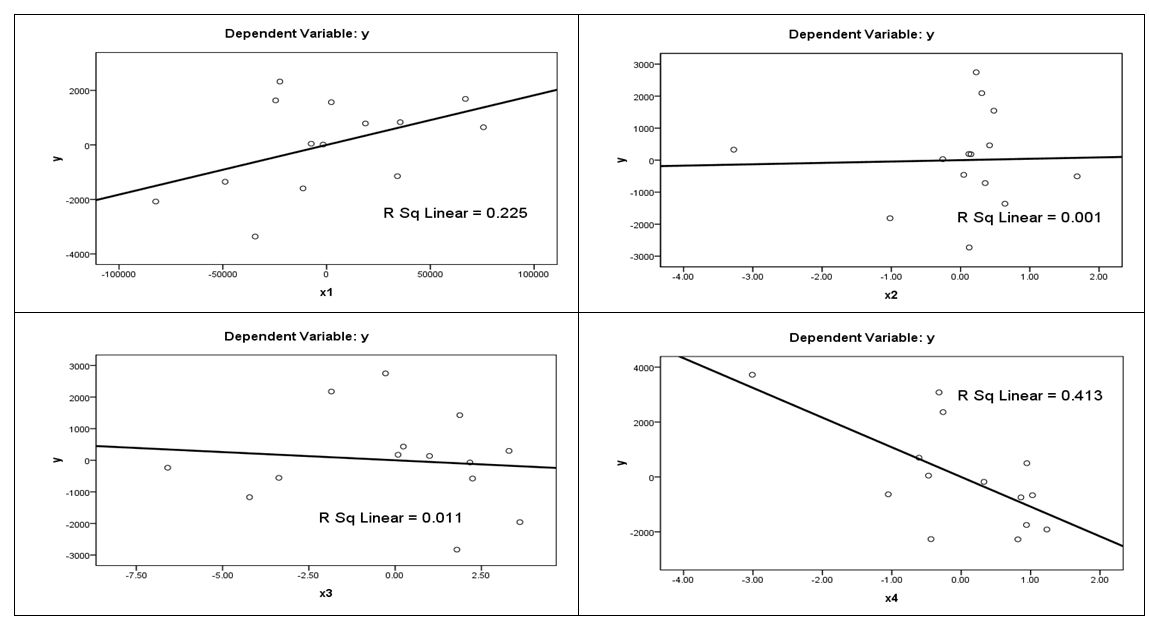
\includegraphics[width=\linewidth]{assets/hospital_partial.png}\end{center}


\par\addvspace{6pt}\noindent\begin{minipage}{\linewidth}

\Question{E17-C6}{高R平方与变量作用排序}

根据表2结果，以下判断哪些正确？

I. 模型决定系数很大，至少有预测应用价值。

\begin{enumerate}
\def\labelenumi{\Roman{enumi}.}
\setcounter{enumi}{1}
\item
  各自变量作用大小依次为X1\textgreater X2\textgreater X3\textgreater X4。
\item
  各自变量作用大小依次为X4\textgreater X1\textgreater X2\textgreater X3。
\end{enumerate}


\begin{choices}

\item 仅I

\item 仅II

\item 仅III

\item I \& III

\item I、II、III均不正确

\end{choices}

\end{minipage}\par\vspace{4pt}

\par\addvspace{6pt}\noindent\begin{minipage}{\linewidth}

\Question{E17-C7}{删去一个变量后的系数}

若Y对X1、X2、X3建模,估计偏回归系数从大到小(不考虑绝对值)排列为


\begin{choices}

\item X1 X3 X2

\item X2 X1 X3

\item X3 X2 X1

\item X1 X2 X3

\item X2 X3 X1

\end{choices}

\end{minipage}\par\vspace{4pt}

\par\addvspace{6pt}\noindent\begin{minipage}{\linewidth}

\Question{E17-C8}{识别强影响观测}

模型的强影响点是OBS


\begin{choices}

\item 4\&11

\item 5

\item 7\&14

\item 14

\item 无强影响点

\end{choices}

\end{minipage}\par\vspace{4pt}

\par\addvspace{6pt}\noindent\begin{minipage}{\linewidth}

\Question{E17-C9}{变量相关不等于误差不独立}

以下哪些说法正确？

I. 根据专业知识，X2和X3不符合LINE中的I条件。

\begin{enumerate}
\def\labelenumi{\Roman{enumi}.}
\setcounter{enumi}{1}
\item
  需要结合偏相关分析判断Y是否独立。
\item
  根据已有统计信息，可断定Y存在序列相关。
\end{enumerate}


\begin{choices}

\item 仅I

\item 仅II

\item 仅III

\item I \& III

\item I、II、III均不正确

\end{choices}

\end{minipage}\par\vspace{4pt}

\par\addvspace{6pt}\noindent\begin{minipage}{\linewidth}

\Question{E17-C10}{住院模型的改进}

本例分析改进的建议,合理的是 I: 将X2剔除\\
II:使用岭回归\\
III:考虑某种时间序列模型


\begin{choices}

\item 仅I

\item 仅II

\item 仅III

\item II \& III

\item I \& II \&III

\end{choices}

\end{minipage}\par\vspace{4pt}

\par\addvspace{6pt}\noindent\begin{minipage}{\linewidth}

\Question{E17-L2}{剔除春节数据后的变化}

如果作者推测春节对急诊量的影响是正确的,则剔除春节期间数据建模,则可能出现的情况是 I. 模型的决定系数变大 II. 偏回归系数的P值变大 III. 偏回归系数绝对值变大


\begin{choices}

\item 仅I

\item 仅II

\item 仅III。

\item I II

\item I III

\item 不能仅据题设确定这些指标的变化方向。

\end{choices}

\end{minipage}\par\vspace{4pt}

\par\addvspace{6pt}\noindent\begin{minipage}{\linewidth}

\Question{E17-L3}{每日资料的独立性风险}

你认为本文存在的致命缺陷是


\begin{choices}

\item 共线性问题导致参数估计结果难以理解

\item 违反线性假设导致模型不``正确''

\item 违反正态性或等方差假设导致参数估计和置信区间不准确

\item 违反独立性假设导致增大I型错误

\item 未给出拟合优度统计量评估模型的应用价值

\end{choices}

\end{minipage}\par\vspace{4pt}

\par\addvspace{6pt}\noindent\begin{minipage}{\linewidth}

\Question{E17-L4}{旧文献的统计表述}

本文论述不妥或错误之处不含


\begin{choices}

\item 关于回代符合率与R2的论述

\item 样本回归方程的书写格式

\item 使用冠心病发病概率的回归模型为线性回归的范例

\item 表1关于假变量(标识变量)的定义

\item 关于共线性的的论述

\end{choices}

\end{minipage}\par\vspace{4pt}

\par\addvspace{6pt}\noindent\begin{minipage}{\linewidth}

\Question{E17-L10}{两年率资料的模型前提}

本文的多重线性回归分析存在的最大问题是


\begin{choices}

\item 婴儿死亡率不服从正态分布

\item 共线性问题

\item 未报告拟合优度统计量

\item 可能不满足独立性假设

\item 未考察线性假设

\end{choices}

\end{minipage}\par\vspace{4pt}

\par\addvspace{6pt}\noindent\begin{minipage}{\linewidth}

\Question{E21-2}{三种残差的分布}

多重线性回归模型,如果满足LINE条件,则 I、标准化残差服从标准正态分布 II、学生化残差服从t分布 III、粗残差估计值均值为0,标准差为剩余标准差


\begin{choices}

\item I

\item II

\item III

\item I\&II\&III

\item 全错

\end{choices}

\end{minipage}\par\vspace{4pt}

\par\addvspace{6pt}\noindent\begin{minipage}{\linewidth}

\Question{E21-4}{正态性是条件假设}

关于回归分析的正态和等方差条件,错误的是


\begin{choices}

\item 给定X条件下Y为正态分布。

\item 可以用Y的边际经验分布与正态分布的吻合判断回归的正态性假设。

\item 可以用粗残差的PP或QQ图初步判断正态性。

\item 可用残差对Y拟合值的散点图判断等方差性。

\item 在模型假设下，不同X取值处的Y条件方差相等。

\end{choices}

\end{minipage}\par\vspace{4pt}

\par\addvspace{6pt}\noindent\begin{minipage}{\linewidth}

\Question{E21-5}{影响点敏感性分析}

多重线性回归统计分析时,发现存在强影响点,则适宜的处理方法是


\begin{choices}

\item 同时报告基于原始数据的模型和删去强影响点的模型

\item 报告更符合自己专业预期的模型

\item 报告基于原始数据的模型

\item 报告删去强影响点的模型

\item 重新收集数据以避免强影响点的影响

\end{choices}

\end{minipage}\par\vspace{4pt}

\par\addvspace{6pt}\noindent\begin{minipage}{\linewidth}

\Question{E21-19}{Durbin–Watson的直接计算}

如果某模型残差依照时间顺序为(0.2, 0.03, 0.4, 0.5, -0.1, 0.02, -0.7, -0.1),则其Durbin-Watson统计量是(拍照没拍全,数据可能不对)


\begin{choices}

\item 0.80

\item 0.89

\item 0.92

\item 0.96

\item 1.11

\item 1.486（按题中所记残差计算）。

\end{choices}

\end{minipage}\par\vspace{4pt}

\par\addvspace{6pt}\noindent\begin{minipage}{\linewidth}

\Question{E21-9}{杠杆与影响度}

关于高杠杆点和强影响点，哪项正确？


\begin{choices}

\item 高杠杆点必有最大粗残差。

\item 高杠杆表示X空间位置特殊，但是否强影响还取决于残差等信息。

\item Cook距离只反映结局绝对大小。

\item 一见高杠杆就必须删除。

\item 杠杆值与自变量无关。

\end{choices}

\end{minipage}\par\vspace{4pt}

\par\addvspace{6pt}\noindent\begin{minipage}{\linewidth}

\Question{N19-8}{VIF与容忍度}

若 \(X_j\) 对其余解释变量回归的 \(R_j^2=.95\)，则VIF为：


\begin{choices}

\item 0.05。

\item 0.95。

\item 1.05。

\item 20。

\item 95。

\end{choices}

\end{minipage}\par\vspace{4pt}

\par\addvspace{6pt}\noindent\begin{minipage}{\linewidth}

\Question{N19-9}{DW的无相关参考值}

残差一阶自相关很弱时，DW通常接近：


\begin{choices}

\item 0。

\item 1。

\item 2。

\item 3。

\item 4。

\end{choices}

\end{minipage}\par\vspace{4pt}

\par\addvspace{6pt}\noindent\begin{minipage}{\linewidth}

\Question{N19-10}{Cook距离的含义}

Cook距离主要衡量：


\begin{choices}

\item 删除单个观测对整体拟合或系数的影响。

\item 某观测的Y值有多大。

\item 某自变量的样本均值。

\item 结局是否正态的P值。

\item 两组样本量差异。

\end{choices}

\end{minipage}\par\vspace{4pt}

\par\addvspace{6pt}\noindent\begin{minipage}{\linewidth}

\Question{N19-11}{正态性检查对象}

回归的经典正态假设主要针对：


\begin{choices}

\item 给定设计后的误差。

\item X的边际分布。

\item Y的边际分布必为单峰正态。

\item X与Y联合必相互独立。

\item 回归系数原始数值。

\end{choices}

\end{minipage}\par\vspace{4pt}

\par\addvspace{6pt}\noindent\begin{minipage}{\linewidth}

\Question{N19-12}{异方差稳健标准误}

采用异方差稳健标准误后，哪项最准确？


\begin{choices}

\item 不改变OLS点估计，仅改变适当条件下的方差估计与推断。

\item 自动修正了遗漏的非线性。

\item 自动消除所有混杂。

\item 使残差必然正态。

\item 让新个体预测永远准确。

\end{choices}

\end{minipage}\par\vspace{4pt}

\par\addvspace{6pt}\noindent\begin{minipage}{\linewidth}

\Question{N19-13}{模型选择与验证泄漏}

在交叉验证中筛选变量、选变换和岭参数，应如何处理？


\begin{choices}

\item 仅在各训练折内完成，再评估验证折。

\item 先用全数据选好，再声称验证完全独立。

\item 只看训练误差最小。

\item 根据验证折结局修改原始数据。

\item 忽略分组或时间结构随机打散所有观测。

\end{choices}

\end{minipage}\par\vspace{4pt}

\par\addvspace{6pt}\noindent\begin{minipage}{\linewidth}

\Question{N19-21}{急诊文章的日均数核查}

按急诊共用资料，199649人次除以730天，平均每日约为：


\begin{choices}

\item 273.49。

\item 274.50。

\item 199.65。

\item 730.00。

\item 285.48。

\end{choices}

\end{minipage}\par\vspace{4pt}

\par\addvspace{6pt}\noindent\begin{minipage}{\linewidth}

\Question{N19-22}{回归系数与标准误}

急诊文中平均相对湿度B=1.011、SE=.159，则检验该系数为0的t值约为：


\begin{choices}

\item 0.157。

\item 0.244。

\item 6.36。

\item 1.011。

\item 无法由这两个数计算。

\end{choices}

\end{minipage}\par\vspace{4pt}

\Needspace{7\baselineskip}\subsubsection*{共用资料：生命质量文章的回归结果}

同文以生命质量总分为结局，报告如下最终多元回归。焦虑/抑郁用原始得分，病程用月，癫痫0否1是，病理分级与文化程度分别按1---4有序编码。

\begin{center}\small\setlength{\tabcolsep}{3.5pt}\renewcommand{\arraystretch}{1.18}\begin{tabular}{@{}lrrrrr@{}}
\toprule
变量 & B & SE & 标准化\(\beta\) & t & P \\
\midrule

截距 & 74.033 & 1.543 & --- & 47.974 & \textless.01 \\
焦虑 & -0.884 & 0.204 & -0.385 & -4.326 & \textless.01 \\
抑郁 & -0.655 & 0.225 & -0.263 & -2.906 & \textless.01 \\
病程 & 0.056 & 0.022 & 0.158 & 2.518 & \textless.05 \\
癫痫 & -4.902 & 1.301 & -0.233 & -3.768 & \textless.01 \\
病理分级 & -0.987 & 0.412 & -0.156 & -2.396 & \textless.05 \\
文化程度 & 0.905 & 0.393 & 0.148 & 2.302 & \textless.05 \\
\bottomrule\end{tabular}\end{center}

文中报告 \(F=22.554\)、\(R^2=.539\)、调整 \(R^2=.517\)。


\par\addvspace{6pt}\noindent\begin{minipage}{\linewidth}

\Question{N19-26}{R平方与调整R平方}

生命质量模型报告R²=.539、调整R²=.517。关于训练样本平方和比例，正确的是：


\begin{choices}

\item 普通R²表示相对于仅截距模型解释了53.9\%的总平方和。

\item 普通R²等于51.7\%。

\item 调整R²保证模型无偏。

\item 该模型已证明外部预测同样好。

\item 余下全部变异均为测量错误。

\end{choices}

\end{minipage}\par\vspace{4pt}

\subsection{简答题}

\par\addvspace{6pt}\noindent\begin{minipage}{\linewidth}

\Question{S20-2}{异方差残差图}

方差不等的典型残差图呈何种形态？手绘示意并简要说明（原题要求提交手绘照片）。


\worklines{3}

\end{minipage}\par\vspace{4pt}

\subsection{计算与分析题}

\Needspace{7\baselineskip}\subsubsection*{共用资料：数学、语文与智商数据}

以智商为y，数学为x1，语文为x2。原卷data1未独立附上，本包补入同课程``语文数学智商.sav''（18人）作数值复算；若原卷数据有改动，需重新代入。


\par\addvspace{6pt}\noindent\begin{minipage}{\linewidth}

\Question{C20-1b}{智商模型的共线性与岭回归}

继续分析智商数据： 1. 计算指标作共线性诊断。 2. 做岭回归、绘制岭迹图，选择岭参数并说明依据。 3. 给出岭参数k=0.12时的原尺度回归方程。


\worklines{3}

\end{minipage}\par\vspace{4pt}

\Needspace{7\baselineskip}\subsubsection*{共用资料：父母与子女身高数据}

y为子女身高，x1为父亲身高，x2为母亲身高。正文同名数据与附带2023 data1逐值一致；以下保留原数据单位，不擅自转换为厘米。

\begin{center}\small\setlength{\tabcolsep}{3.5pt}\renewcommand{\arraystretch}{1.18}\begin{tabular}{@{}lrrr@{}}
\toprule
观测 & 父x1 & 母x2 & 子y \\
\midrule

1 & 5.2 & 4.9 & 6.2 \\
2 & 5.4 & 5.1 & 5.9 \\
3 & 6.2 & 5.5 & 6.6 \\
4 & 5.8 & 5.4 & 6 \\
5 & 5.6 & 5.1 & 6.2 \\
6 & 5 & 4.9 & 5.6 \\
7 & 6.4 & 5.6 & 6.6 \\
8 & 6 & 5.4 & 6.5 \\
\bottomrule\end{tabular}\end{center}


\par\addvspace{6pt}\noindent\begin{minipage}{\linewidth}

\Question{C21-1b}{身高模型的岭迹与k=0.11}

对身高数据： 1. 计算共线性指标。 2. 绘制岭迹图，选岭参数并说明理由。 3. 给出k=0.11时的岭回归方程。


\worklines{3}

\end{minipage}\par\vspace{4pt}

\par\addvspace{6pt}\noindent\begin{minipage}{\linewidth}

\Question{C19-1}{父母身高的岭回归复习题}

对父母子身高数据进行共线性分析，再作岭回归、选择岭参数并写出回归模型。


\worklines{3}

\end{minipage}\par\vspace{4pt}

\par\addvspace{6pt}\noindent\begin{minipage}{\linewidth}

\Question{C19-2}{非线性关系与LINE诊断}

原题给一个SPSS文件，含4个自变量和1个因变量，要求拟合多重线性回归并诊断LINE。回忆提示某个自变量与结局明显呈反比例关系，需用1/x替换后重新拟合。

原4自变量文件未附；这里改用正文中的``线性假设诊断''数据（3个解释变量），只作方法演示。


\worklines{3}

\end{minipage}\par\vspace{4pt}

\Needspace{7\baselineskip}\subsubsection*{共用资料：1990—2003年住院人次及模型诊断}

\begin{center}\small\setlength{\tabcolsep}{3.5pt}\renewcommand{\arraystretch}{1.18}\begin{tabular}{@{}lrrrrr@{}}
\toprule
年份 & 住院人次Y & 门诊X1 & 周转率X2 & 使用率X3 & 住院日X4 \\
\midrule

1990 & 11501 & 454220 & 14.42 & 93.38 & 24.14 \\
1991 & 11512 & 496556 & 14.43 & 90.81 & 23.73 \\
1992 & 11504 & 480663 & 14.36 & 90.31 & 23.73 \\
1993 & 11841 & 445274 & 14.11 & 88.75 & 22.64 \\
1994 & 12096 & 427614 & 9.1 & 82.84 & 22.46 \\
1995 & 11648 & 461228 & 13.92 & 82.53 & 21.93 \\
1996 & 11622 & 391975 & 13.84 & 81.15 & 21.6 \\
1997 & 14892 & 439554 & 17.81 & 92.05 & 19.12 \\
1998 & 18928 & 533686 & 22.82 & 91.86 & 15.08 \\
1999 & 21651 & 605660 & 23.13 & 91.84 & 14.68 \\
2000 & 24673 & 597541 & 24.74 & 91.61 & 13.5 \\
2001 & 28305 & 592311 & 25.1 & 88.63 & 12.7 \\
2002 & 27864 & 590564 & 24.6 & 85.98 & 12.58 \\
2003 & 28691 & 756273 & 27.2 & 84.56 & 12.18 \\
\bottomrule\end{tabular}\end{center}

X2为年出院人数/床位数；X3为占用总床日数/开放总床日数；X4为平均住院日。原表2：

\begin{center}\small\setlength{\tabcolsep}{3.5pt}\renewcommand{\arraystretch}{1.18}\begin{tabular}{@{}lrrrrr@{}}
\toprule
变量 & B & SE & 标准化\(\beta\) & t & P \\
\midrule

截距 & 33058.528 & 12905.767 & --- & 2.562 & 0.031 \\
X1 & 0.0176 & 0.011 & 0.243 & 1.569 & 0.151 \\
X2 & 45.151 & 445.16 & 0.034 & 0.095 & 0.927 \\
X3 & -56.103 & 162.181 & -0.032 & -0.346 & 0.737 \\
X4 & -1100.129 & 436.507 & -0.736 & -0.52 & 0.033 \\
\bottomrule\end{tabular}\end{center}

原表报告 \(R^2=.958\)，调整 \(R^2=.939\)。以下诊断也按原卷保留。

\begin{center}\small\setlength{\tabcolsep}{3.5pt}\renewcommand{\arraystretch}{1.18}\begin{tabular}{@{}lrrrr@{}}
\toprule
观测 & 残差 & 残差标准误 & Student残差 & Cook D \\
\midrule

1 & 1525 & 1449 & 1.052 & 0.109 \\
2 & 186.8319 & 1492.8 & 0.125 & 0.001 \\
3 & 445.4631 & 1536.9 & 0.29 & 0.006 \\
4 & 178.2094 & 1651.5 & 0.108 & 0 \\
5 & 468.4283 & 446.7 & 1.049 & 3.238 \\
6 & -1388 & 1503.1 & -0.924 & 0.066 \\
7 & -577.5792 & 1093.9 & -0.528 & 0.09 \\
8 & -460.7536 & 1498.2 & -0.308 & 0.008 \\
9 & -2734 & 1555.1 & -1.758 & 0.184 \\
10 & -1770 & 1539.1 & -1.15 & 0.086 \\
11 & 43.0857 & 1576.1 & 0.0273 & 0 \\
12 & 2735 & 1575.9 & 1.735 & 0.158 \\
13 & 2080 & 1537.1 & 1.353 & 0.12 \\
14 & -730.8267 & 892.2 & -0.819 & 0.395 \\
\bottomrule\end{tabular}\end{center}

\begin{center}\small\setlength{\tabcolsep}{3.5pt}\renewcommand{\arraystretch}{1.18}\begin{tabular}{@{}lr@{}}
\toprule
变量 & VIF \\
\midrule

X1 & 5.13579 \\
X2 & 27.61614 \\
X3 & 1.87395 \\
X4 & 17.71312 \\
\bottomrule\end{tabular}\end{center}

\begin{center}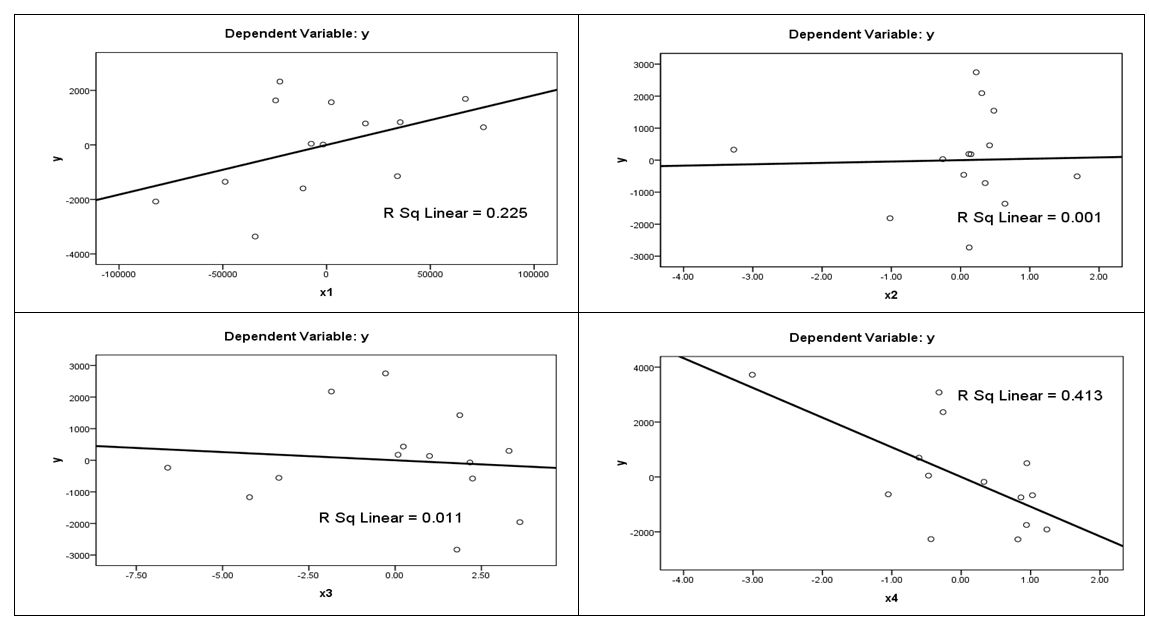
\includegraphics[width=\linewidth]{assets/hospital_partial.png}\end{center}


\par\addvspace{6pt}\noindent\begin{minipage}{\linewidth}

\Question{C20-2}{住院人次：逐步回归与诊断}

以y为住院人次，x1---x4的定义见共用资料，对data2作逐步回归。 1. 写出最终回归方程和拟合优度。 2. 计算指标考察独立性。 3. 列出最大的中心化杠杆、学生化残差、Cook距离及对应观测（原稿此句末尾缺失，本书按年份及数值补齐）。


\worklines{3}

\end{minipage}\par\vspace{4pt}

\par\addvspace{6pt}\noindent\begin{minipage}{\linewidth}

\Question{C21-2}{住院人次：偏回归图与时间顺序}

对同定义的住院data2资料作逐步回归。 1. 写出回归方程和拟合优度。 2. 绘图作线性诊断。 3. 计算指标考察独立性。 4. 列出最大的中心化杠杆、学生化残差、Cook距离，给出年份与数值。


\worklines{3}

\end{minipage}\par\vspace{4pt}



\clearpage\section{补充练习}

本节为配合正文新编的补充练习，按题型排列，题号接续本章往年题，解析见章末。

\subsection{单项选择题}

\par\addvspace{6pt}\noindent\begin{minipage}{\linewidth}

\Question{X26-2-1}{DW检验的不确定区间}

对有时间顺序的资料作回归，得到 \(DW=1.30\)。按题设检验水平、样本量及自变量数查表得 \(d_L=1.10\)、\(d_U=1.50\)。根据正文给出的DW区间判定法，最恰当的结论是：


\begin{choices}

\item 已证实存在一阶正自相关。

\item 已证实存在一阶负自相关。

\item 已证实不存在一阶自相关。

\item DW小于2，因此必定违反所有LINE条件。

\item 对一阶正自相关的判定不确定，需进一步考察。

\end{choices}

\end{minipage}\par\vspace{4pt}

\par\addvspace{6pt}\noindent\begin{minipage}{\linewidth}

\Question{X26-2-2}{条件指数与VIF的联合判断}

三个解释变量的相关阵特征值为2.500、0.499、0.001，其中 \(X_1\) 对其余两个解释变量回归的 \(R_1^2=0.96\)。以下说法正确的是：


\begin{choices}

\item 最大条件指数为2500，\(VIF_1=0.04\)。

\item 最大条件指数为50，说明相关阵必不可逆。

\item 最大条件指数为50，\(VIF_1=25\)，提示严重但非完全共线性。

\item 容忍度为25，说明共线性很弱。

\item 只要3个特征值之和为3，就不存在共线性。

\end{choices}

\end{minipage}\par\vspace{4pt}

\par\addvspace{6pt}\noindent\begin{minipage}{\linewidth}

\Question{X26-2-3}{按相关阵计算岭系数}

两个解释变量与结局均已标准化，给定 \[R_{XX}=\begin{pmatrix}1&0.9\\0.9&1\end{pmatrix},\qquad
r_{XY}=\begin{pmatrix}0.8\\0.7\end{pmatrix}.\] 按正文定义 \(b^*(k)=(R_{XX}+kI)^{-1}r_{XY}\)，取 \(k=0.10\)。两个标准化岭系数依次为：


\begin{choices}

\item \((0.8947,-0.1053)\)。

\item \((0.6250,0.1250)\)。

\item \((0.8000,0.7000)\)。

\item \((0.1250,0.6250)\)。

\item \((0.7273,0.6364)\)。

\end{choices}

\end{minipage}\par\vspace{4pt}

\subsection{简答题}

\Question{X26-2-4}{偏回归图的代码纠错}

要考察控制 \(X_2,X_4\) 后 \(X_3\) 与Y的线性关系，某同学写出：

\begin{verbatim}
u <- resid(lm(x3 ~ x2 + x4, data = d))
v <- resid(lm(y ~ x2 + x3 + x4, data = d))
plot(u, v)
\end{verbatim}

假设资料无缺失、模型满列秩。指出代码中的关键问题，写出正确代码，并说明为什么原图可能让人误判为``X3与Y无关''。


\worklines{3}

\subsection{计算与分析题}

\Question{X26-2-5}{小样本的离群与杠杆诊断}

对下列数据拟合含截距的一元线性回归：

\begin{center}\small\setlength{\tabcolsep}{5pt}\renewcommand{\arraystretch}{1.18}\begin{tabular}{@{}llllll@{}}
\toprule
观测号 & 1 & 2 & 3 & 4 & 5 \\
\midrule

X & 1 & 2 & 3 & 4 & 5 \\
Y & 3.4 & 7.9 & 14.6 & 13.6 & 15.5 \\
\bottomrule\end{tabular}\end{center}

本题按正文经验标准筛查：\(|r_{i(\text{外})}|>3\) 提示Y方向离群；\(h_{ii}>2\bar h\) 提示高杠杆；Cook \(D_i>1\) 提示强影响。

\begin{enumerate}
\def\labelenumi{\arabic{enumi}.}
\tightlist
\item
  给出回归方程、剩余标准差及第3号观测的粗残差、杠杆值、内学生化残差、外学生化残差、Cook距离；据此判断第3号观测。
\item
  加入第6号观测 \((X_6,Y_6)=(10,33)\) 后重新拟合，计算第6号观测的杠杆值、外学生化残差、Cook距离，并判断其属于哪类可疑观测。
\item
  说明两问的结果为何不矛盾，以及发现可疑观测后的处理原则。
\end{enumerate}


\worklines{3}

\clearpage\section{习题解析}

\begin{keyidea}[核对方式]题号与前文一一对应。补写范围、原题歧义及数据还原方法列在相应答案中。\end{keyidea}

\Answer{E14-14}{拟合优度与应用价值}

\textbf{答案：E。}

R²是否有用取决于领域、目标和验证表现，没有通用0.8或0.9门槛。加入变量会使训练R²不降，不能单靠最大化它筛选；调整R²也不是无条件无偏或预测可靠性的证明。


\Answer{E14-15}{回归的前提条件}

\textbf{答案：C。}

回归并不要求结局与自变量相互独立，否则通常也无关系可建模。独立性主要指给定设计后观测误差相互独立；正态性用于经典小样本推断，正态假定针对条件误差而不是边际Y。


\Answer{E14-16}{文献报告不足与已证实错误}

\textbf{答案：E较符合``不包括''的意图。}

未展示散点图不能证明作者没有检查过线性，且线性应结合专业关系、函数形式和残差/偏残差考察。文章确实未报告本模型拟合优度；表中SE中文写成``标准物''是笔误。时间相关及共线性是应检查的风险，不能在无原始数据时声称已由检验证实。


\Answer{E14-17}{讨论与模型是否一致}

\textbf{答案：D。}

讨论提到高温和低温都可能增加急症，而拟合式以最高、最低气温的正线性项描述关系，并未给出U形等非线性证据。应区分研究自身模型结果与引用或推测，避免把讨论中的机制解释当成已验证结果。


\Answer{E14-19}{原文统计表述辨析}

\textbf{答案：待原文核实。}

选项涉及文章对拟合优度、模型前提、哑变量和系数的具体陈述；原文未附，无法可靠指定错误项。可核对条件分布而非边际正态、参照编码以及概率与优势的区别。


\Answer{E14-20}{率的变换与分析}

\textbf{答案：C是通常可接受的方法选项，仍需原文核实。}

对比例作平方根反正弦变换是传统可用方法之一，本身不能直接定为错误；是否适合还取决于分母、边界与方差结构。两年同一单位的率可能相关，且统计关联不能证明降低出生率会降低婴儿死亡率。


\Answer{E14-21}{将伴随关系解释为因果}

\textbf{答案：D。}

若仅凭观察性回归即说降低出生率能够降低婴儿死亡率，属于把关联上升为因果干预效果。原文未附，能够评价的是选项所描述的推论，不能断言文章其他部分是否还有更大问题。


\Answer{E17-M3}{LINE中的独立性}

\textbf{答案：B。}

指不同观察单位的误差在给定自变量后独立；不是Y与X独立，也不是各自变量必须独立。B是原选项最接近的表述。


\Answer{E17-M5}{独立性如何判断}

\textbf{答案：B（一般情形）。}

独立性首先取决于抽样和研究设计。对有时间顺序的数据，DW和残差时序图是辅助诊断，因此A、D在相应场景也有用；任何单一图或检验都不能证明任意依赖形式不存在。


\Answer{E17-M9}{R平方的使用}

\textbf{答案：E。}

小R²也可能有研究或预测价值，但仍须评估误差、校准及验证。统计显著不自动等于重要，调整R²也不保证无偏。


\Answer{E17-M13}{预测价值的证据}

\textbf{答案：C。}

独立外部样本上的预测误差最有说服力。训练残差、R²或学生化残差都不能替代对新数据的预测评估；数据预处理与选择也不能泄漏外部样本信息。


\Answer{E17-M14}{强影响点的处理}

\textbf{答案：A。}

先核对录入、测量和样本是否符合纳入规则；无确证错误时不随意删除。报告包含与不包含该点的敏感性分析，说明系数、结论如何变化，避免按预期结果选模型。


\Answer{E17-M15}{等方差的图形诊断}

\textbf{答案：E。}

看残差相对拟合值或自变量的散点，漏斗形等模式提示方差随均值改变。


\Answer{E17-M17}{控制智商后的成绩关系}

\textbf{答案：C。}

分别剔除智商等协变量的线性作用后，可用偏回归/残差散点考察两科成绩的条件关系。


\Answer{E17-M18}{正态性的图形诊断}

\textbf{答案：D。}

应看模型残差的QQ图，重点是条件误差分布；不能只看原始Y的边际分布。


\Answer{E17-C6}{高R平方与变量作用排序}

\textbf{答案：E。}

高训练R²本身不证明预测价值。变量量纲不同，且X2/X4共线性严重、有强影响点，不能据单次全模型系数直接确定稳健贡献排序；III即便符合表中标准化绝对值排序，也不等于可靠的因果或预测贡献。


\Answer{E17-C7}{删去一个变量后的系数}

\textbf{答案：B。}

对原表1转录资料拟合 \(Y\sim X_1+X_2+X_3\)，得到系数约0.01054、1057.35、−311.08，因此按代数值降序为 \(X_2>X_1>X_3\)。不要按旧模型系数直接删除一项而不重新拟合。


\Answer{E17-C8}{识别强影响观测}

\textbf{答案：B。}

原输出第5个观测Cook D约3.238，明显突出；该点对应1994年。其学生化残差未必很大，因为高杠杆点可将回归面拉向自身。


\Answer{E17-C9}{变量相关不等于误差不独立}

\textbf{答案：E。}

LINE中的I不是要求自变量之间独立。偏相关不能检验时间序列误差独立；原给诊断不足以断定序列相关存在。应结合按时间排列的残差及适当检验。


\Answer{E17-C10}{住院模型的改进}

\textbf{答案：E（作为可研究的候选方案）。}

核对并考虑移除冗余变量、使用岭回归缓解不稳定，以及处理年度时间结构，都是可比较的改进方向。删除X2须有依据并重新拟合；岭回归不自动解决序列相关，时间序列模型也不自动解决错误函数形式。


\Answer{E17-L2}{剔除春节数据后的变化}

\textbf{答案：F（补入：无法仅据题设确定）。}

删除部分日期可能改变暴露分布、残差方差、样本量和系数，因此R²、P值、系数绝对值没有必然方向。需要原数据与明确的节假日效应模型，不能凭叙述决定I/II/III。


\textbf{补写说明。} 原B、C选项均写``仅II''，这里将C补为``仅III''，并加入无法确定变化方向的F项；不宣称F来自原卷。


\Answer{E17-L3}{每日资料的独立性风险}

\textbf{答案：D（优先需要检查的风险）。}

730个连续日期可能存在趋势、季节性或残差自相关；若被忽略，标准误和检验可能不可靠。但论文未给时间残差诊断，不能在没有数据时说已检验证实违反独立性。


\Answer{E17-L4}{旧文献的统计表述}

\textbf{答案：待原文核实。}

选项须对照原文关于线性概率模型、回代符合率、变量赋值和共线性的实际表述；本包未提供该文，不能指定唯一正确项。


\Answer{E17-L10}{两年率资料的模型前提}

\textbf{答案：D是题目提示的主要风险，需原文核验。}

若同一民族或地区提供两个年份的率，它们可能相关，不能简单视为独立观察。原文未附，尚不能确认该研究具体数据结构或其余问题是否更严重。


\Answer{E21-2}{三种残差的分布}

\textbf{答案：B若指外学生化；E若指内部学生化。}

含截距时残差均值为0，但其样本标准差与剩余标准差分别为\[\sqrt{SSE/(n-1)},\qquad s=\sqrt{SSE/(n-p-1)},\]二者不相等，所以III通常错误。以估计的s标准化的残差不严格为标准正态。删点外学生化残差在经典正态模型下有精确t分布；内部学生化不服从该t分布。原稿把II一律判错混淆了定义。


\Answer{E21-4}{正态性是条件假设}

\textbf{答案：B。}

给定X的条件误差正态，不要求混合了不同条件均值的边际Y正态。粗残差QQ图可作初步诊断；杠杆差异大时标准化/学生化更有帮助，但不能说粗残差QQ图本身就是错误。原回忆稿的对错批注不正确。


\Answer{E21-5}{影响点敏感性分析}

\textbf{答案：A。}

先核对录入、测量和样本是否符合纳入规则；无确证错误时不随意删除。报告包含与不包含该点的敏感性分析，说明系数、结论如何变化，避免按预期结果选模型。


\Answer{E21-19}{Durbin–Watson的直接计算}

\textbf{答案：F（补入1.486）。}

按回忆向量，\(DW=\sum_{i=2}^n(e_i-e_{i-1})^2/\sum_{i=1}^n e_i^2=1.4286/0.9613\approx1.48611\)。原A---E均不匹配，说明回忆向量或选项有缺误。保留原向量和选项，补入本向量对应值；R应写 \texttt{sum(diff(e)\^{}2)/sum(e\^{}2)}，避免矩阵乘除优先级错误。


\textbf{补写说明。} 保留回忆残差与原A---E，新增与所记向量一致的F项。原稿注明残差可能没记全。


\Answer{E21-9}{杠杆与影响度}

\textbf{答案：B。}

杠杆来自设计矩阵。强影响常是杠杆与残差共同作用，需检查删除该点后估计如何改变。


\textbf{补写说明。} 原第9题整题未记录，本题新编。


\Answer{N19-8}{VIF与容忍度}

\textbf{答案：D。}

\(VIF=1/(1-R_j^2)=20\)，容忍度0.05。阈值是经验诊断，不应单靠它删去关键变量。


\textbf{补写说明。} 2019回忆稿只给出30道选择的总数及大致范围，没有记录本题原文；本题是依课程内容与所附材料新编的补充练习，不冒作恢复的原试卷。


\Answer{N19-9}{DW的无相关参考值}

\textbf{答案：C。}

近似关系为 \(DW\approx2(1-\hat\rho_1)\)；正式判定仍需对应设计的分布或检验，不能用2作机械界线。


\textbf{补写说明。} 2019回忆稿只给出30道选择的总数及大致范围，没有记录本题原文；本题是依课程内容与所附材料新编的补充练习，不冒作恢复的原试卷。


\Answer{N19-10}{Cook距离的含义}

\textbf{答案：A。}

它结合残差与杠杆信息。可疑观测应核查并作敏感性分析，不宜为得到显著结果而删除。


\textbf{补写说明。} 2019回忆稿只给出30道选择的总数及大致范围，没有记录本题原文；本题是依课程内容与所附材料新编的补充练习，不冒作恢复的原试卷。


\Answer{N19-11}{正态性检查对象}

\textbf{答案：A。}

不同X对应不同条件均值，混合后边际Y可以不呈正态。残差图用于近似诊断，不能把它当独立误差的直接观测。


\textbf{补写说明。} 2019回忆稿只给出30道选择的总数及大致范围，没有记录本题原文；本题是依课程内容与所附材料新编的补充练习，不冒作恢复的原试卷。


\Answer{N19-12}{异方差稳健标准误}

\textbf{答案：A。}

稳健标准误解决的是方差估计问题，不能替代正确均值模型或因果设计。


\textbf{补写说明。} 2019回忆稿只给出30道选择的总数及大致范围，没有记录本题原文；本题是依课程内容与所附材料新编的补充练习，不冒作恢复的原试卷。


\Answer{N19-13}{模型选择与验证泄漏}

\textbf{答案：A。}

所有利用结局的选择都应在训练阶段进行；相关资料还需按个体、组或时间块划分，必要时采用嵌套验证。


\textbf{补写说明。} 2019回忆稿只给出30道选择的总数及大致范围，没有记录本题原文；本题是依课程内容与所附材料新编的补充练习，不冒作恢复的原试卷。


\Answer{N19-21}{急诊文章的日均数核查}

\textbf{答案：A。}

直接相除为273.4918，与文中274.5不一致，应核查总数、天数或报告值。


\textbf{补写说明。} 2019回忆稿只给出30道选择的总数及大致范围，没有记录本题原文；本题是依课程内容与所附材料新编的补充练习，不冒作恢复的原试卷。


\Answer{N19-22}{回归系数与标准误}

\textbf{答案：C。}

\(t=B/SE\approx6.3585\)；但其标称P值是否可靠还取决于误差相关结构等条件。


\textbf{补写说明。} 2019回忆稿只给出30道选择的总数及大致范围，没有记录本题原文；本题是依课程内容与所附材料新编的补充练习，不冒作恢复的原试卷。


\Answer{N19-26}{R平方与调整R平方}

\textbf{答案：A。}

调整R²加入自由度惩罚，不能简单替代原始平方和比例；两者也都不等于样本外表现。


\textbf{补写说明。} 2019回忆稿只给出30道选择的总数及大致范围，没有记录本题原文；本题是依课程内容与所附材料新编的补充练习，不冒作恢复的原试卷。


\Answer{S20-2}{异方差残差图}

常见为漏斗形或喇叭形：残差中心仍大致围绕0，但随拟合值或某自变量变化，竖向散布逐渐增大或减小。

\begin{center}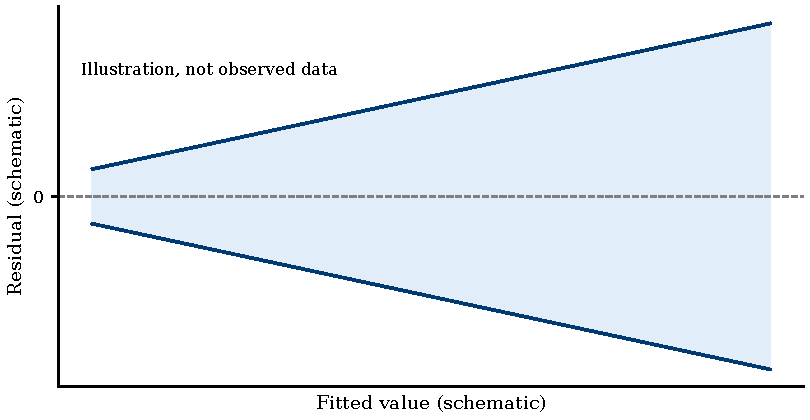
\includegraphics[width=.82\linewidth]{assets/funnel_schematic.pdf}\end{center}

这是数学示意的散布包络，不是实测样本点。还可能出现其他异方差模式，不能只寻找一种形状；需结合变量变换、方差建模或稳健标准误，并先确保均值函数合适。


\Answer{C20-1b}{智商模型的共线性与岭回归}

本书统一采用相关阵尺度的岭参数定义： \[b^*(k)=(R_{XX}+kI)^{-1}r_{XY},\quad b_j(k)=b_j^*(k)\frac{s_Y}{s_{X_j}},\quad b_0(k)=\bar Y-\sum_jb_j(k)\bar X_j.\] 其他软件若以 \(X^TX+\lambda I\) 定义惩罚，参数量级会不同，不能直接混用。

相关系数0.932002；容忍度0.131372；两个变量VIF均为7.611995。以相关阵特征根比平方根定义的条件指数约5.3304。

\begin{center}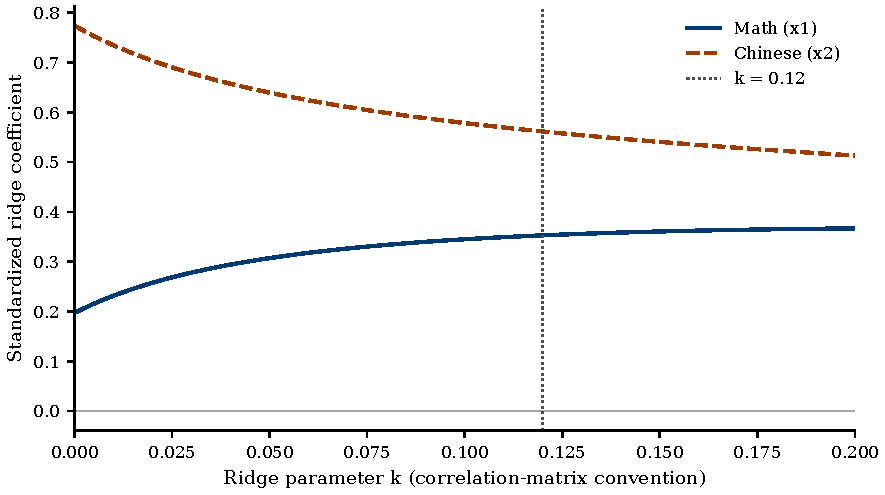
\includegraphics[width=.9\linewidth]{assets/ridge_iq.pdf}\end{center}

k=0.12的原尺度方程为 \[\widehat y=12.092095+0.387816x_1+0.713526x_2.\] 在0---0.20、步长0.005的预设网格中，GCV最小在k=0.04；它与题目指定的0.12不是同一要求。岭迹趋稳可作为辅助，但不应只为让系数``好看''选参数。图中为实算的标准化系数路径，完整网格随代码提供。


\Answer{C21-1b}{身高模型的岭迹与k=0.11}

本书统一采用相关阵尺度的岭参数定义： \[b^*(k)=(R_{XX}+kI)^{-1}r_{XY},\quad b_j(k)=b_j^*(k)\frac{s_Y}{s_{X_j}},\quad b_0(k)=\bar Y-\sum_jb_j(k)\bar X_j.\] 其他软件若以 \(X^TX+\lambda I\) 定义惩罚，参数量级会不同，不能直接混用。

父母身高相关0.974782；容忍度0.049799；VIF均为20.080645；条件指数约8.8493。

\begin{center}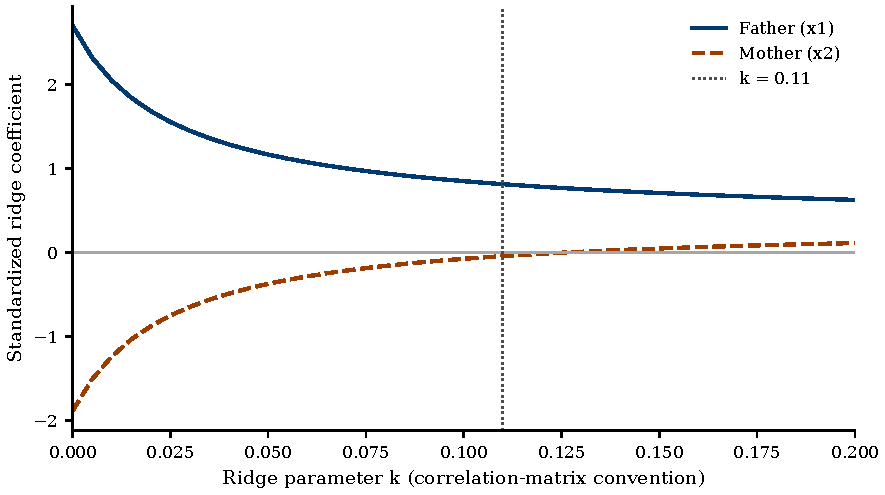
\includegraphics[width=.9\linewidth]{assets/ridge_height.pdf}\end{center}

k=0.11时 \[\widehat y=3.095451+0.595344x_1-0.055162x_2.\] 此时标准化系数为(0.813395,−0.041879)。按每0.01一个k、首列k=0的存储方式，k=0.11应取第12列，不能误取第11列。

\textbf{选参的限制。} 在本包0---0.20、步长0.005网格中，GCV最小在k=0；这与``曲线变稳定''标准不同。因此可以报告正k下的稳定性分析，但不能声称0.11在该数据上已经证明预测最优。


\Answer{C19-1}{父母身高的岭回归复习题}

本书统一采用相关阵尺度的岭参数定义： \[b^*(k)=(R_{XX}+kI)^{-1}r_{XY},\quad b_j(k)=b_j^*(k)\frac{s_Y}{s_{X_j}},\quad b_0(k)=\bar Y-\sum_jb_j(k)\bar X_j.\] 其他软件若以 \(X^TX+\lambda I\) 定义惩罚，参数量级会不同，不能直接混用。

原2019数据未另附，采用正文同名的8条记录演示：VIF约20.0806，说明父母身高的条件系数不稳定。岭迹及原尺度换算可按本章身高题操作。

如指定k=0.11作稳定性展示，方程为 \(\hat y=3.095451+0.595344x_1-0.055162x_2\)；若严格按本包粗网格GCV选择，最小点为k=0，即普通最小二乘。应说明选择标准和小样本局限，而不是把某个正k当作唯一标准答案。


\Answer{C19-2}{非线性关系与LINE诊断}

先检查散点和控制其他变量后的偏残差关系，再检查设计独立性、残差正态与方差结构；同时看异常/强影响点。若专业及图形支持反比例关系，可用 \(1/X_j\) 作为解释项，注意 \(X_j=0\) 的定义和近零值的不稳定性，再重复诊断与验证。

正文3自变量演示数据中，将x1改为倒数使AIC由397.682降至390.610，方程为 \[\hat y=347.5607-606.6008/x_1+4.5034x_2+1.9687x_3.\] 这些数字不冒作2019原卷4自变量的结果；原文件补齐后应按同样步骤分析，不能把case编号作为解释变量凑数。


\Answer{C20-2}{住院人次：逐步回归与诊断}

本包依据原卷表1逐格转录的14年数据，用AIC的双向逐步法，保留x1、x4： \[\widehat y=28825.883+0.0185703x_1-1122.3837x_4.\] \(R^2=0.956916\)，调整 \(R^2=0.949082\)，剩余标准差1613.316。按年份排列残差，\(DW=1.064356\)；\texttt{lmtest::dwtest}双侧P约0.00829，提示该模型的序列相关问题值得处理。

最大中心化杠杆 \(h_i-1/n\) 在2003年，为0.551061；最大绝对外学生化残差在1998年，为−2.30630；代数最大的外学生化残差在2001年，为2.21072；最大Cook D也在2001年，为0.309879。必须说明按绝对值还是代数值选``最大''。

\textbf{版本核对。} 原表2系数与表1转录复算不完全一致，且表中X4的t写作−0.520，与系数/标准误约−2.520不符。旧卷data2没有独立文件，这里明确以可见表1为复算依据；若找到原卷文件，应重新核对。全部逐步选择、残差和年份指标已随代码提供。


\Answer{C21-2}{住院人次：偏回归图与时间顺序}

本包依据原卷表1逐格转录的14年数据，用AIC的双向逐步法，保留x1、x4： \[\widehat y=28825.883+0.0185703x_1-1122.3837x_4.\] \(R^2=0.956916\)，调整 \(R^2=0.949082\)，剩余标准差1613.316。按年份排列残差，\(DW=1.064356\)；\texttt{lmtest::dwtest}双侧P约0.00829，提示该模型的序列相关问题值得处理。

最大中心化杠杆 \(h_i-1/n\) 在2003年，为0.551061；最大绝对外学生化残差在1998年，为−2.30630；代数最大的外学生化残差在2001年，为2.21072；最大Cook D也在2001年，为0.309879。必须说明按绝对值还是代数值选``最大''。

\textbf{版本核对。} 原表2系数与表1转录复算不完全一致，且表中X4的t写作−0.520，与系数/标准误约−2.520不符。旧卷data2没有独立文件，这里明确以可见表1为复算依据；若找到原卷文件，应重新核对。全部逐步选择、残差和年份指标已随代码提供。

最终模型的偏回归图（控制另一个保留变量，14个年份）：

\begin{center}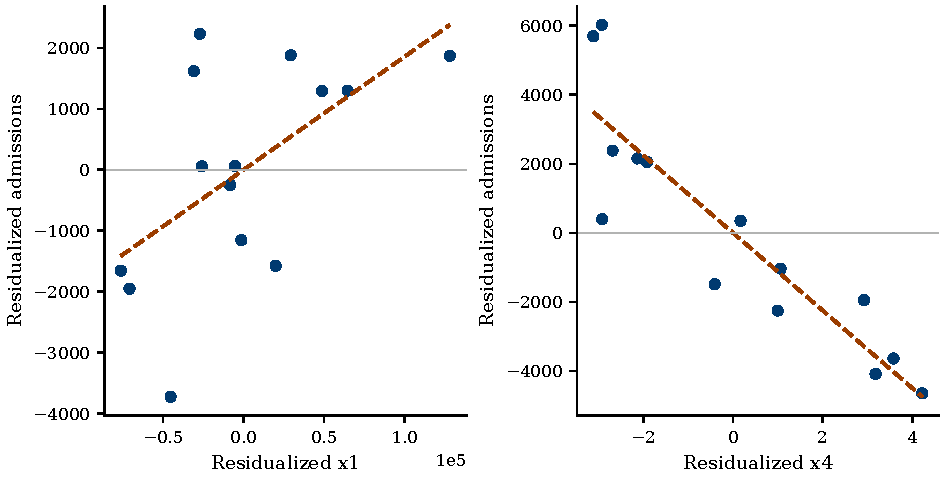
\includegraphics[width=\linewidth]{assets/hospital_partial_recomputed.pdf}\end{center}

直线只作条件关系的图形参照。仅有总体趋势不足以证明线性形式正确；应同时看曲率、影响观测与时间残差，并区分原全模型的偏回归图和这里最终模型的图。

\clearpage\subsection*{补充练习解析}

以下为补充练习的解析。这些题目为配合正文新编，并非往年试题；题中设定的数值仅供练习。

\Answer{X26-2-1}{DW检验的不确定区间}

\textbf{答案：E。}

\(d_L<DW<d_U\)，落在不能确定的区间。\(DW<2\) 可提示正相关方向，但不能替代查表结论，更不能把``不确定''当作``没有自相关''。可继续查看按时间排列的残差图，并采用适合该资料的进一步检验。




\Answer{X26-2-2}{条件指数与VIF的联合判断}

\textbf{答案：C。}

按正文相关阵定义，最大条件指数为 \(\sqrt{2.500/0.001}=50\)；\(VIF_1=1/(1-0.96)=25\)，容忍度0.04。两项均提示严重共线性，但最小特征值仍大于0，不能称为完全共线性。系数可能不稳定，不等于正规方程已无唯一解。




\Answer{X26-2-3}{按相关阵计算岭系数}

\textbf{答案：B。}

\[b^*(0.10)=\frac1{1.1^2-0.9^2}
\begin{pmatrix}1.1&-0.9\\-0.9&1.1\end{pmatrix}
\begin{pmatrix}0.8\\0.7\end{pmatrix}
=\begin{pmatrix}0.625\\0.125\end{pmatrix}.\] 岭惩罚加在计算矩阵的主对角线上，原始变量的样本相关系数仍为0.9。它改变的是估计方法；本题给定的k也不代表已由岭迹选出了最佳参数。




\Answer{X26-2-4}{偏回归图的代码纠错}

第二个辅助回归不应包含待考察的 \(X_3\)；两边都只剔除控制变量 \(X_2,X_4\) 的线性影响。

\begin{verbatim}
u <- resid(lm(x3 ~ x2 + x4, data = d))
v <- resid(lm(y ~ x2 + x4, data = d))
plot(u, v)
abline(lm(v ~ u))
\end{verbatim}

原代码的v是完整回归的残差，与设计矩阵各列正交；u又是这些列的线性组合，故样本内 \(u^Tv=0\)。原图中的线性趋势被构造过程消掉，不能据此说X3没有条件效应。正确图用于考察控制其他变量后的线性关系；图形本身也不是已证明LINE全部成立。




\Answer{X26-2-5}{小样本的离群与杠杆诊断}

\textbf{（1）原5点模型。} \(\hat Y=2.03+2.99X\)，\(s=2.4453\)。第3号观测的结果为：

\begin{center}\small\setlength{\tabcolsep}{5pt}\renewcommand{\arraystretch}{1.18}\begin{tabular}{@{}ll@{}}
\toprule
指标 & 数值 \\
\midrule

粗残差 & 3.6000 \\
杠杆值 & 0.2000 \\
内学生化残差 & 1.6460 \\
外学生化残差 & 4.3164 \\
Cook距离 & 0.3386 \\
\bottomrule\end{tabular}\end{center}

因此第3号按题设标准提示Y方向离群，但其杠杆不高，Cook距离也未超过1。不能仅因内学生化残差未超过3就忽略它。

\textbf{（2）加入第6号后。} 新方程为 \(\hat Y=1.6967+3.1128X\)，\(s=2.1288\)。第6号 \(h_{66}=0.8361\)，\(\bar h=2/6=0.3333\)，故 \(h_{66}>2\bar h\)；其外学生化残差0.1772、Cook距离0.1056。它提示高杠杆，但按题设阈值不提示Y方向离群或强影响。判断须使用6点模型的诊断量。

\textbf{（3）区别与处理。} 外学生化残差以删点后估计的误差方差衡量Y方向偏离；杠杆反映X位置是否特殊；Cook距离综合残差与杠杆。本例第6号虽在X方向较远，却贴近回归线。经验阈值用于筛查，应先核查数据，再比较含该点与不含该点的拟合，不按是否有利于结论选择性删点。

可用R的 \texttt{rstandard()}、\texttt{rstudent()}、\texttt{hatvalues()}、\texttt{cooks.distance()} 复算，完整代码随笔记提供。
\EndExercises

\chapter{一般线性模型}
完全随机设计、随机区组设计、析因设计的方差分析与协方差分析，通常各有一套平方和公式。本章将它们统一表述为线性模型$Y=X\beta+\varepsilon$，各种设计的区别仅在于设计矩阵$X$的构成：分组因素以哑变量列表示，协变量为数值列，交互作用为相应列的乘积。第2、3章关于最小二乘估计、$t$检验、增量$F$检验与模型诊断的内容均适用于本章。

对每一种设计，可从以下三方面理解：
\begin{enumerate}
\item 设计矩阵包含哪些列，即模型的写法；
\item 各系数的含义，它取决于编码方式，参照组编码与效应编码给出的系数不同；
\item 误差项包含哪些变异。随机区组设计将窝别差异从误差中分离，协方差分析将年龄的作用从误差中分离，误差减小，检验效能随之提高。
\end{enumerate}
第三点体现了试验设计的基本原则：通过合理设计，使误差中只保留无法控制的随机变异。
\section{一般线性模型概述}
一般线性模型（General Linear Model，GLM）是一种用于分析因变量与一个或多个自变量之间线性关系的统计模型。它通过建立变量间的线性关系，利用最小二乘法估计参数，从而解释或预测因变量的变化。
\begin{enumerate}
\item 应用范围：不仅包含线性回归，还涵盖方差分析、协方差分析等模型。
\item 参数估计：通常采用最小二乘法，但在数据存在异方差或非正态分布时可能使用更复杂方法。
\item 建模目的：既可用于预测变量间关系，也可用于假设检验，如组间均值差异。
\end{enumerate}
一般线性模型与多重线性回归是同一个模型$Y=X\beta+\varepsilon$：多重线性回归本来就可以通过哑变量纳入分类自变量，通过变量变换、多项式项和交互项刻画非线性关系与效应修饰。称“一般线性模型”时，通常强调自变量中含有分类因素，把方差分析、协方差分析统一写成回归形式。其因变量仍为连续变量，假设为误差独立、正态、等方差（即第3章的LINE条件）。

须与广义线性模型（Generalized Linear Model，常缩写为GLM或GLiM）区分：后者允许因变量服从二项、Poisson等指数族分布，并通过连接函数$g(E(Y))=X\beta$建立联系，如logistic回归、Poisson回归。二者英文缩写相同，阅读软件文档时须留意。

一般线性模型广泛应用于医学、金融、社会科学等领域，尤其适合需要同时分析连续和分类自变量或进行复杂假设检验的研究。
\section{完全随机设计方差分析}
例1：为研究饮食对小鼠肥胖的干预作用，将30只肥胖小鼠随机等分为3组，每组10只，分别给予普通饮食NR、高大豆蛋白饮食HSP、高猪肉蛋白饮食HPP，进行为期12周的膳食干预，记录前后小鼠体重的变化值（g）。
\question{三种不同喂养方式对肥胖小鼠体重变化值的影响有无差别？}
\par\noindent\begin{minipage}{\linewidth}
\tbltitle{表1\quad 三种不同喂养方式下小鼠体重变化值（g）}
\begin{center}\begin{tabular}{crrrr}
\toprule &$\mathrm{NR}$组&$\mathrm{HSP}$组&$\mathrm{HPP}$组&合计\\\midrule
\multirow{10}{*}{$X_{ij}$}&3.98&1.98&2.68&\\
&5.51&2.83&4.02&\\&4.93&2.30&3.46&\\&5.92&3.20&4.40&\\
&5.54&2.86&4.05&\\&5.39&2.72&3.90&\\&5.20&2.55&3.72&\\
&6.14&3.04&4.61&\\&5.95&3.23&4.43&\\&5.80&3.10&4.29&\\\midrule
$n_i$&10&10&10&$30\ (N)$\\
$\bar X_i$&5.4360&2.7810&3.9560&$4.0577\ (\bar X)$\\
$S_i$&.6304&.4062&.5683&$1.2229\ (S)$\\\bottomrule
\end{tabular}\end{center}
\end{minipage}\par\medskip

\ann{分类变量需进行哑变量化。}
\subsection{参数化}
\[
y_{ij}=\mu_{i}+\varepsilon_{ij},\qquad
y=X\beta+\varepsilon,\quad i=1,2,3,\quad j=1,\ldots,10.
\]
\par\noindent\begin{rcode}
x <- c(3.98,5.51,4.93,5.92,5.54,5.39,5.20,6.14,5.95,5.80,   # NR
       1.98,2.83,2.30,3.20,2.86,2.72,2.55,3.04,3.23,3.10,   # HSP
       2.68,4.02,3.46,4.40,4.05,3.90,3.72,4.61,4.43,4.29)   # HPP
g <- factor(rep(1:3,each=10))
\end{rcode}\par\smallskip
不含截距的模型（单元均数参数化，$\beta_i=\mu_i$）：
\par\noindent\begin{rcode}
lm(x~g-1)
\end{rcode}\par\smallskip
\[
\widehat\beta=\begin{bmatrix}\widehat\beta_1\\\widehat\beta_2\\\widehat\beta_3\end{bmatrix}
=\begin{bmatrix}5.436\\2.781\\3.956\end{bmatrix},
\]
即三组样本均数，是总体均数$\mu_1,\mu_2,\mu_3$的估计值。

包含总体均数与组效应项的模型：
\[
\mu_i=\mu+\alpha_i,\qquad
\beta=\begin{bmatrix}\mu\\\alpha_1\\\alpha_2\\\alpha_3\end{bmatrix}.
\]
设计矩阵$X_\mu$的第1列等于后3列之和，$\rank(X_\mu)=3<4$（秩亏），$X_\mu^\top X_\mu$不可逆，$\mu$与各$\alpha_i$不能唯一确定：对任意$c$，$(\mu+c,\alpha_i-c)$给出完全相同的$\mu_i$。须加一个约束才能唯一求解：
\begin{itemize}
\item 和为零约束$\sum_i\alpha_i=0$（效应编码，\code{contr.sum}）：$\mu=\frac13\sum\mu_i$为各组总体均数的平均，$\alpha_i=\mu_i-\mu$为第$i$组相对于平均水平的效应。本例$\widehat\mu=4.0577$，$\widehat\alpha=(1.3783,\,-1.2767,\,-0.1017)$。各组例数相等时$\widehat\mu$就是30个观测的均数。
\item 参考组约束$\alpha_1=0$（R默认的\code{contr.treatment}）：截距为参考组均数$\mu_1$，其余系数为与参考组之差。
\end{itemize}
\ann{$\mu$为30个观测的总体平均，$\alpha_i$为组效应项；\code{mean(y1)-mean(y)}。有的资料称“此模型只能手算，因为后面的列完全共线”：秩亏模型软件同样可以处理，\code{lm}会对冗余列给出\code{NA}（相当于令其系数为0），加约束或改用上述编码即可唯一求解。}
\par\noindent\begin{rcode}
X_mu <- cbind(1,model.matrix(~g-1))   # 设计矩阵X_mu
qr(X_mu)$rank                         # 3：4列但秩为3
lm(x~X_mu-1)                          # 冗余的最后一列系数为NA
options(contrasts=c("contr.sum","contr.poly")); lm(x~g)   # 和为零编码
options(contrasts=c("contr.treatment","contr.poly"))       # 恢复默认
\end{rcode}\par\smallskip
\Needspace{6\baselineskip}
以第1组为参照：
\par\noindent\begin{rcode}
lm(x~g)
\end{rcode}\par\smallskip
\[
\gamma_0=\mu+\alpha_1=\mu_1,\qquad
\gamma_2=\alpha_2-\alpha_1=\mu_2-\mu_1,\qquad\gamma_3=\alpha_3-\alpha_1=\mu_3-\mu_1.
\]
\[
(\widehat\gamma_0,\widehat\gamma_2,\widehat\gamma_3)=(\mathrm{Intercept},g2,g3)=(5.436,-2.655,-1.480).
\]
\ann{$\gamma_2$为第2组与第1组的效应差，$\gamma_3$为第3组与第1组的效应差。为避免与回归系数向量$\beta$混淆，参考组编码下的系数记为$\gamma$。}
\textbf{可估计性。}线性函数$c^\top\beta$称为可估计的，若存在$a$使$c^\top\beta=a^\top E(Y)=a^\top X\beta$对一切$\beta$成立，即$c^\top$位于$X$的行空间内。秩亏模型中，$\mu_i=\mu+\alpha_i$、组间差$\alpha_2-\alpha_1$以及一般的对比$\sum c_i\alpha_i$（$\sum c_i=0$）都可估计；$\mu$与单个$\alpha_i$不可估计，其数值取决于所加的约束。
\begin{derivation}{列空间相同的参数化给出相同的拟合与对比}
\dpart{条件}两个设计矩阵$X_1$、$X_2$的列空间相同（如上面的$X_0$、$X_\mu$、$X_{\mathrm{ref}}$，或任意一种对比编码），可以满秩，也可以秩亏。
\dpart{结论}两者的拟合值、残差、残差平方和以及据此构造的$F$检验完全相同；任何可估计函数的估计值相同。
\dpart{推导}最小二乘拟合值$\widehat Y$是在列空间$\mathcal C(X)$中离$Y$最近的点，即$Y$在$\mathcal C(X)$上的正交投影。投影只由子空间决定，与用哪组列向量（以及秩亏时用哪个广义逆、哪种约束）表示该子空间无关，故$\widehat Y$、$e=Y-\widehat Y$相同。可估计函数$c^\top\beta=a^\top X\beta=a^\top E(Y)$的最小二乘估计为$a^\top\widehat Y$，只依赖$\widehat Y$，因此也相同。
\dpart{统计解释}三种写法下，第2组与第1组之差都估计为$2.781-5.436=-2.655$；变的只是参数的名字与含义。解读系数前必须先弄清所用的编码。
\end{derivation}
{\small\setlength{\arraycolsep}{3.5pt}\renewcommand{\arraystretch}{.75}\[X_0=\begin{bmatrix}1&0&0\\1&0&0\\1&0&0\\1&0&0\\1&0&0\\1&0&0\\1&0&0\\1&0&0\\1&0&0\\1&0&0\\0&1&0\\0&1&0\\0&1&0\\0&1&0\\0&1&0\\0&1&0\\0&1&0\\0&1&0\\0&1&0\\0&1&0\\0&0&1\\0&0&1\\0&0&1\\0&0&1\\0&0&1\\0&0&1\\0&0&1\\0&0&1\\0&0&1\\0&0&1\end{bmatrix},\qquad X_\mu=\begin{bmatrix}1&1&0&0\\1&1&0&0\\1&1&0&0\\1&1&0&0\\1&1&0&0\\1&1&0&0\\1&1&0&0\\1&1&0&0\\1&1&0&0\\1&1&0&0\\1&0&1&0\\1&0&1&0\\1&0&1&0\\1&0&1&0\\1&0&1&0\\1&0&1&0\\1&0&1&0\\1&0&1&0\\1&0&1&0\\1&0&1&0\\1&0&0&1\\1&0&0&1\\1&0&0&1\\1&0&0&1\\1&0&0&1\\1&0&0&1\\1&0&0&1\\1&0&0&1\\1&0&0&1\\1&0&0&1\end{bmatrix},\qquad X_{\mathrm{ref}}=\begin{bmatrix}1&0&0\\1&0&0\\1&0&0\\1&0&0\\1&0&0\\1&0&0\\1&0&0\\1&0&0\\1&0&0\\1&0&0\\1&1&0\\1&1&0\\1&1&0\\1&1&0\\1&1&0\\1&1&0\\1&1&0\\1&1&0\\1&1&0\\1&1&0\\1&0&1\\1&0&1\\1&0&1\\1&0&1\\1&0&1\\1&0&1\\1&0&1\\1&0&1\\1&0&1\\1&0&1\end{bmatrix}.\]}
\subsection{检验过程}
\[
H_0:\alpha_1=\alpha_2=\alpha_3=0;\qquad
H_1:\text{至少有一个效应项不为0},\qquad\alpha=0.05.
\]
\par\noindent\begin{minipage}{\linewidth}
\tbltitle{表7-4\quad 案例7-1资料的方差分析表}
\begin{center}\begin{tabular}{lrrrrr}
\toprule 变异来源&$SS$&$\nu$&$MS$&$F$&$P$\\\midrule
总变异&43.3685&29&&&\\
组间变异&35.4002&2&17.7001&59.9800&$<.05$\\
组内变异&7.9683&27&.2951&&\\\bottomrule
\end{tabular}\end{center}
\end{minipage}\par\medskip

\[
F=\frac{\ms{组间}}{\ms{组内}}=59.98\sim F(2,27),\qquad P<0.05.
\]
按0.05水准拒绝$H_0$，接受$H_1$，认为至少两组的干预作用有不同。
\begin{sikao}[$F$检验后的多重比较]
方差分析的$F$检验只能判断各组总体均数是否全部相等。拒绝$H_0$后，需进一步确定哪些组之间存在差异及差异的大小，即进行多重比较。常用Tukey法，它将“三对比较中至少犯一次第一类错误”的概率控制在0.05：
\par\noindent\begin{rcode}
g <- factor(rep(c("NR","HSP","HPP"),each=10),levels=c("NR","HSP","HPP"))
TukeyHSD(aov(x~g))
\end{rcode}
\begin{routput}
          diff        lwr        upr     p adj
HSP-NR  -2.655 -3.2573759 -2.0526241 0.0000000
HPP-NR  -1.480 -2.0823759 -0.8776241 0.0000049
HPP-HSP  1.175  0.5726241  1.7773759 0.0001362
\end{routput}
三对比较均有统计学意义：普通饮食组体重变化最大，高大豆蛋白组最小。其中差值$-2.655$、$-1.480$即参照组编码中$\gamma_2$、$\gamma_3$的估计值，区别仅在于置信区间按多重比较作了加宽。

多组比较不宜直接进行多次$t$检验。每次检验犯第一类错误的概率为0.05，进行3次比较时，至少犯一次第一类错误的概率最高可达$1-0.95^3\approx0.14$。组数越多，该概率越大（5组共10对比较，约为0.40）。
\end{sikao}
\par\noindent\begin{minipage}{\linewidth}
\tbltitle{完全随机设计方差分析的变异分解表}
\begin{center}\small\setlength{\tabcolsep}{5pt}\begin{tabular}{ccccc}
\toprule 来源&平方和&自由度&均方的期望&$F$\\\midrule
组间&$\sum_i n_i(\bar Y_{i\cdot}-\bar Y)^2$&$a-1$&$\sigma^2+\dfrac{\sum n_i\alpha_i^2}{a-1}$&$\dfrac{\ms{组间}}{\ms{组内}}$\\[8pt]
组内&$\sum_i\sum_j(Y_{ij}-\bar Y_{i\cdot})^2$&$N-a$&$\sigma^2$&\\[4pt]
总&$\sum_i\sum_j(Y_{ij}-\bar Y)^2$&$N-1$&&\\\bottomrule
\end{tabular}\end{center}
（均方期望中的$\alpha_i$按$\sum n_i\alpha_i=0$定义。）
\end{minipage}\par\medskip

\[
\ms{处理}=\frac{\SSq{处理}}{a-1},\qquad
\ms{组内}=\frac{\SSq{组内}}{N-a}.
\]
\ann{$a$为组数，$N$为实验对象总数。}
\section{随机区组设计方差分析}
两因素方差分析，无交互作用。

例2：为研究某改良型富血小板纤维蛋白（A-PRF）在软骨再生中的作用，建立兔膝关节软骨缺损模型，选取造模成功的8窝，每窝3只，共24只兔子。按窝别将每窝3只随机分配到三个处理组，在缺损处分别给予植入A-PRF、植入A-PRF+BMSCs（骨髓间充质干细胞）、不植入三种处理。手术后12周处死兔，采用国际软骨修复协会宏观评估评分（ICRS评分）评估再生组织的质量。
\question{不同植入方式间ICRS评分是否不同？}
\ann{有的资料称“两步随机”：先分到8窝，每窝内再随机处理方法。更准确地说，8窝是既有的区组，兔子按出生窝别自然归入区组，并非随机分配形成；随机化只有一步，即在每窝内将3只兔随机分配到三种处理。每个格子（窝$\times$处理）只有1个观测，处理与区组的交互作用和纯随机误差无法分别估计；下面的检验采用可加模型，假定处理效应在各窝间相同，若存在交互作用则被并入误差项。}
\par\noindent\begin{minipage}{\linewidth}
\tbltitle{不同植入方式下兔软骨修复ICRS评分}
\begin{center}\begin{tabular}{crrr}
\toprule 区组&植入A-PRF&植入A-PRF+BMSCs&不植入\\\midrule
1&5.97&7.12&4.42\\2&9.92&9.37&5.56\\3&8.00&7.68&7.53\\
4&11.25&10.51&8.90\\5&9.53&9.47&7.63\\6&10.01&9.03&7.12\\
7&8.88&8.48&6.48\\8&11.95&11.19&9.64\\\bottomrule
\end{tabular}\end{center}
\end{minipage}\par\medskip

\subsection{模型与参数估计}
可加模型（$i$为处理，$a=3$；$j$为区组，$n=8$）：
\[
y_{ij}=\mu+\alpha_i+\beta_j+\varepsilon_{ij},\qquad\sum_i\alpha_i=0,\quad\sum_j\beta_j=0,
\quad i=1,2,3,\quad j=1,\ldots,8 .
\]
记$\mu_{i\cdot}$、$\mu_{\cdot j}$分别为第$i$个处理、第$j$个区组的总体均数，在和为零约束下$\alpha_i=\mu_{i\cdot}-\mu$，$\beta_j=\mu_{\cdot j}-\mu$。最小二乘估计为
\[
\widehat\mu=\bar y_{\cdot\cdot},\qquad
\widehat\alpha_i=\bar y_{i\cdot}-\bar y_{\cdot\cdot},\qquad
\widehat\beta_j=\bar y_{\cdot j}-\bar y_{\cdot\cdot},\qquad
e_{ij}=y_{ij}-\bar y_{i\cdot}-\bar y_{\cdot j}+\bar y_{\cdot\cdot}.
\]
\ann{$\widehat\mu$为所有24个数据的均数（本例8.5683）；$\widehat\alpha_i$为处理效应估计，$\widehat\beta_j$为区组效应估计。下面的全组哑变量设计矩阵$X_{\mathrm{all}}$有12列，秩为$1+2+7=10$，需加约束或改用参照组编码；\code{lm}可直接拟合，冗余列给出\code{NA}。}
以第一窝且植入A-PRF兔子的平均ICRS为参照（参照组编码，系数记为$\gamma$）：
\begin{align*}
\gamma_0&=\mu+\alpha_1+\beta_1=E(y_{11}),\\
\gamma_{\mathrm{treat}i}&=\alpha_i-\alpha_1=\mu_{i\cdot}-\mu_{1\cdot},\quad i=2,3,\\
\gamma_{\mathrm{block}j}&=\beta_j-\beta_1=\mu_{\cdot j}-\mu_{\cdot1},\quad j=2,\ldots,8.
\end{align*}
可加模型下，处理差$\alpha_i-\alpha_1$在每一窝中都相同，所以无需指明是哪一窝。
\par\noindent\begin{rcode}
y <- c(5.97,9.92,8.00,11.25,9.53,10.01,8.88,11.95,   # 植入A-PRF
       7.12,9.37,7.68,10.51,9.47,9.03,8.48,11.19,    # A-PRF+BMSCs
       4.42,5.56,7.53,8.90,7.63,7.12,6.48,9.64)      # 不植入
treat <- factor(rep(1:3,each=8)); block <- factor(rep(1:8,3))
mean(y)
aggregate(y,by=list(treat),mean)
X <- model.matrix(~treat+block)
solve(t(X)%*%X)%*%t(X)%*%y
lm(y~treat+block)
\end{rcode}\par\smallskip
{\footnotesize\setlength{\arraycolsep}{2.5pt}\renewcommand{\arraystretch}{.78}
\[X_{\mathrm{all}}=\begin{bmatrix}1&1&0&0&1&0&0&0&0&0&0&0\\1&1&0&0&0&1&0&0&0&0&0&0\\1&1&0&0&0&0&1&0&0&0&0&0\\1&1&0&0&0&0&0&1&0&0&0&0\\1&1&0&0&0&0&0&0&1&0&0&0\\1&1&0&0&0&0&0&0&0&1&0&0\\1&1&0&0&0&0&0&0&0&0&1&0\\1&1&0&0&0&0&0&0&0&0&0&1\\1&0&1&0&1&0&0&0&0&0&0&0\\1&0&1&0&0&1&0&0&0&0&0&0\\1&0&1&0&0&0&1&0&0&0&0&0\\1&0&1&0&0&0&0&1&0&0&0&0\\1&0&1&0&0&0&0&0&1&0&0&0\\1&0&1&0&0&0&0&0&0&1&0&0\\1&0&1&0&0&0&0&0&0&0&1&0\\1&0&1&0&0&0&0&0&0&0&0&1\\1&0&0&1&1&0&0&0&0&0&0&0\\1&0&0&1&0&1&0&0&0&0&0&0\\1&0&0&1&0&0&1&0&0&0&0&0\\1&0&0&1&0&0&0&1&0&0&0&0\\1&0&0&1&0&0&0&0&1&0&0&0\\1&0&0&1&0&0&0&0&0&1&0&0\\1&0&0&1&0&0&0&0&0&0&1&0\\1&0&0&1&0&0&0&0&0&0&0&1\end{bmatrix},\quad\beta=\begin{bmatrix}\mu\\\alpha_1\\\alpha_2\\\alpha_3\\\beta_1\\\beta_2\\\beta_3\\\beta_4\\\beta_5\\\beta_6\\\beta_7\\\beta_8\end{bmatrix}.\]
\[X_{\mathrm{ref}}=\begin{bmatrix}1&0&0&0&0&0&0&0&0&0\\1&0&0&1&0&0&0&0&0&0\\1&0&0&0&1&0&0&0&0&0\\1&0&0&0&0&1&0&0&0&0\\1&0&0&0&0&0&1&0&0&0\\1&0&0&0&0&0&0&1&0&0\\1&0&0&0&0&0&0&0&1&0\\1&0&0&0&0&0&0&0&0&1\\1&1&0&0&0&0&0&0&0&0\\1&1&0&1&0&0&0&0&0&0\\1&1&0&0&1&0&0&0&0&0\\1&1&0&0&0&1&0&0&0&0\\1&1&0&0&0&0&1&0&0&0\\1&1&0&0&0&0&0&1&0&0\\1&1&0&0&0&0&0&0&1&0\\1&1&0&0&0&0&0&0&0&1\\1&0&1&0&0&0&0&0&0&0\\1&0&1&1&0&0&0&0&0&0\\1&0&1&0&1&0&0&0&0&0\\1&0&1&0&0&1&0&0&0&0\\1&0&1&0&0&0&1&0&0&0\\1&0&1&0&0&0&0&1&0&0\\1&0&1&0&0&0&0&0&1&0\\1&0&1&0&0&0&0&0&0&1\end{bmatrix},\quad\gamma=\begin{bmatrix}\gamma_0\\\gamma_{\mathrm{treat}2}\\\gamma_{\mathrm{treat}3}\\\gamma_{\mathrm{block}2}\\\gamma_{\mathrm{block}3}\\\gamma_{\mathrm{block}4}\\\gamma_{\mathrm{block}5}\\\gamma_{\mathrm{block}6}\\\gamma_{\mathrm{block}7}\\\gamma_{\mathrm{block}8}\end{bmatrix}.\]
}
\par\noindent\begin{minipage}{\linewidth}
\tbltitle{模型参数估计结果}
\begin{center}\small\begin{tabular}{lrr}
\toprule 参数&矩阵计算&\code{lm}输出\\\midrule
Intercept&6.707083&6.7071\\
treat2&$-.332500$&$-.3325$\\
treat3&$-2.278750$&$-2.2788$\\
block2&2.446667&2.4467\\
block3&1.900000&1.9000\\
block4&4.383333&4.3833\\
block5&3.040000&3.0400\\
block6&2.883333&2.8833\\
block7&2.110000&2.1100\\
block8&5.090000&5.0900\\\bottomrule
\end{tabular}\end{center}
\end{minipage}\par\medskip

\subsection{变异分解}
\begin{align*}
y_{ij}&=\bar y_{\cdot\cdot}+(\bar y_{i\cdot}-\bar y_{\cdot\cdot})+(\bar y_{\cdot j}-\bar y_{\cdot\cdot})
+(y_{ij}-\bar y_{i\cdot}-\bar y_{\cdot j}+\bar y_{\cdot\cdot}),\\
y_{ij}-\bar y_{\cdot\cdot}&=\widehat\alpha_i+\widehat\beta_j+e_{ij},\\
\sum_{i=1}^a\sum_{j=1}^n(y_{ij}-\bar y_{\cdot\cdot})^2
&=n\sum_{i=1}^a(\bar y_{i\cdot}-\bar y_{\cdot\cdot})^2+a\sum_{j=1}^n(\bar y_{\cdot j}-\bar y_{\cdot\cdot})^2
+\sum_{i=1}^a\sum_{j=1}^n(y_{ij}-\bar y_{i\cdot}-\bar y_{\cdot j}+\bar y_{\cdot\cdot})^2.
\end{align*}
三部分两两正交，交叉项求和为0。前两项的系数$n$、$a$分别是每个处理、每个区组包含的观测数。
\par\noindent\begin{minipage}{\linewidth}
\tbltitle{随机区组设计方差分析的变异分解表}
\begin{center}\small\setlength{\tabcolsep}{4pt}\begin{tabular}{ccccc}
\toprule 来源&平方和&自由度&均方的期望&$F$\\\midrule
处理&$n\sum_i(\bar Y_{i\cdot}-\bar Y)^2$&$a-1$&$\sigma^2+\dfrac{n\sum\alpha_i^2}{a-1}$&$\dfrac{\ms{处理}}{\ms{误差}}$\\[8pt]
区组&$a\sum_j(\bar Y_{\cdot j}-\bar Y)^2$&$n-1$&$\sigma^2+\dfrac{a\sum\beta_j^2}{n-1}$&$\dfrac{\ms{区组}}{\ms{误差}}$\\[8pt]
误差&$\sum_i\sum_j(Y_{ij}-\bar Y_{i\cdot}-\bar Y_{\cdot j}+\bar Y)^2$&$(n-1)(a-1)$&$\sigma^2$&\\[4pt]
总&$\sum_i\sum_j(Y_{ij}-\bar Y)^2$&$na-1$&&\\\bottomrule
\end{tabular}\end{center}
\end{minipage}\par\medskip

\[
\ms{处理}=\frac{\SSq{处理}}{a-1},\quad
\ms{区组}=\frac{\SSq{区组}}{n-1},\quad
\ms{误差}=\frac{\SSq{误差}}{\nu_{\text{误差}}}.
\]
\ann{处理自由度为组数减1；区组自由度为每组个数减1。}
误差自由度可由模型的秩得到：可加模型的设计矩阵秩为$1+(a-1)+(n-1)=a+n-1$，残差自由度为$an-(a+n-1)=(a-1)(n-1)$，本例为$2\times7=14$。若在每格一个观测时再加入处理$\times$区组交互项，模型秩将等于观测数$an$，残差自由度为0，误差方差无从估计。
\subsection{处理因素的检验}
\[
H_0:\alpha_1=\alpha_2=\alpha_3=0;\qquad H_1:\text{至少有一个}\alpha\ne0,\quad\alpha=.05.
\]
\par\noindent\begin{rcode}
anova(lm(y~treat+block))
\end{rcode}\par\smallskip
\begin{center}\small\begin{tabular}{lrrrrr}
\toprule &Df&Sum Sq&Mean Sq&F value&$\Pr(>F)$\\\midrule
treat&2&24.243&12.1215&26.354&$1.793\times10^{-5}\ (***)$\\
block&7&51.088&7.2982&15.867&$1.152\times10^{-5}\ (***)$\\
Residuals&14&6.439&.4600&&\\\bottomrule
\end{tabular}\end{center}
\[
F=\frac{\ms{处理}}{\ms{误差}}=26.354\sim F(2,14),\qquad P<.05.
\]
按0.05水准拒绝$H_0$，接受$H_1$，认为三种植入方式的ICRS评分总体均数不全相同。三种处理的均数依次为9.439、9.106、7.160。
\begin{sikao}[区组的作用]
若忽略窝别，将同一资料按完全随机设计分析，结果如下：
\par\noindent\begin{rcode}
anova(lm(y~treat))         # 忽略区组
\end{rcode}
\begin{routput}
          Df Sum Sq Mean Sq F value  Pr(>F)  
treat      2 24.243 12.1215  4.4249 0.02491 *
Residuals 21 57.527  2.7394                  
\end{routput}
处理平方和24.243不变，误差均方由0.460增至2.739，$F$值由26.35降至4.42。其原因在于窝间差异（平方和51.088）全部计入了误差。同窝兔子的遗传背景与体质相近，窝间差异较大，这部分变异与处理无关，却会掩盖处理效应。

随机区组设计将已知的较大变异来源设为区组，在区组内比较处理，从而将这部分变异从误差中分离。配对$t$检验是其在两组时的特例。若区组间差异不大，单独估计区组效应会多消耗$n-1$个自由度，反而略有损失。

分析方法应与设计相符。随机区组设计的资料若按完全随机设计分析，即使本例结论方向未变，标准误也是错误的。
\end{sikao}
\section{析因设计方差分析}
两因素方差分析，考虑交互。

例3：治疗缺铁性贫血病人12例，分为4组给予不同治疗，一个月后观察红细胞增加数（百万/mm$^3$）。现欲研究甲乙药单独使用的疗效如何，同时使用的疗效又如何（倪宗瓒，《医学统计学》第二版，92页）。
\ann{《医学统计学》194页；平衡设计资料，一型与三型结果等价。}
\par\noindent\begin{minipage}{\linewidth}
\tbltitle{甲乙药治疗后的红细胞增加数（百万/mm$^3$）}
\begin{center}\begin{tabular}{ccrr}
\toprule &&\multicolumn{2}{c}{甲药}\\\cmidrule(lr){3-4}
乙药&&用&不用\\\midrule
\multirow{3}{*}{用}&&2.1&.9\\&&2.2&1.1\\&&2.0&1.0\\\midrule
\multirow{3}{*}{不用}&&1.3&.8\\&&1.2&.9\\&&1.1&.7\\\bottomrule
\end{tabular}\end{center}
\end{minipage}\par\medskip

\par\noindent\begin{minipage}{\linewidth}
\tbltitle{数据格式}
\begin{center}\small\begin{tabular}{rrrrrr}
\toprule $a$&$b$&drug\_a&drug\_b&$y$&PRE\_1\\\midrule
1&1&1&1&2.1&2.10\\1&1&1&1&2.2&2.10\\1&1&1&1&2.0&2.10\\
1&0&1&2&1.3&1.20\\1&0&1&2&1.2&1.20\\1&0&1&2&1.1&1.20\\
0&1&2&1&.9&1.00\\0&1&2&1&1.1&1.00\\0&1&2&1&1.0&1.00\\
0&0&2&2&.8&.80\\0&0&2&2&.9&.80\\0&0&2&2&.7&.80\\\bottomrule
\end{tabular}\end{center}
\end{minipage}\par\medskip

\begin{center}\small\begin{tabular}{rrrr}
\toprule 编号&druga&drugb&rbc\\\midrule
1&1.00&1.00&2.10\\2&1.00&1.00&2.20\\3&1.00&1.00&2.00\\
4&1.00&.00&1.30\\5&1.00&.00&1.20\\
$\cdots$&$\cdots$&$\cdots$&$\cdots$\\\bottomrule
\end{tabular}\end{center}
\par\noindent\begin{rcode}
y <- c(2.1,2.2,2.0, 1.3,1.2,1.1, 0.9,1.1,1.0, 0.8,0.9,0.7)
a <- factor(rep(c(1,2),each=6))         # 甲药：1=用，2=不用
b <- factor(rep(c(1,2,1,2),each=3))     # 乙药：1=用，2=不用
\end{rcode}\par\smallskip
\subsection{交互作用}
\ann{$A$为列均数，$B$为行均数。}
方差分析中的交互作用（Interaction effect）是指两个或多个因素共同影响因变量时，一个因素对因变量的影响会因另一个因素的水平不同而发生变化的现象。交互作用反映因素之间是否存在“联合效应”或“依赖关系”。
\begin{center}\begin{tikzpicture}[font=\footnotesize]
\begin{scope}[shift={(0.0,0.0)}]
\draw (0,0)--(2.9,0);\draw (0,0)--(0,2.1);
\draw[draw=ChartForest,dashed,line width=.9pt] (.3,1.4)--(2.2,1.4);
\draw[draw=ChartBrick,line width=.9pt] (.3,1.25)--(2.2,1.25);
\draw[draw=ChartForest,fill=white] (0.3,1.4) circle (.04);
\draw[draw=ChartForest,fill=white] (2.2,1.4) circle (.04);
\fill[ChartBrick] (0.3,1.25) circle (.035);
\fill[ChartBrick] (2.2,1.25) circle (.035);
\node[right,text=ChartForest] at (2.2,1.6) {B1};\node[right,text=ChartBrick] at (2.2,1.05) {B2};
\node[below] at (.3,0){A1};\node[below] at (2.2,0){A2};
\node[align=left,right] at (3.1,1.1) {A=不显著\\B=不显著};\end{scope}
\begin{scope}[shift={(0.0,-3.3)}]
\draw (0,0)--(2.9,0);\draw (0,0)--(0,2.1);
\draw[draw=ChartForest,dashed,line width=.9pt] (.3,1.6)--(2.2,1.6);
\draw[draw=ChartBrick,line width=.9pt] (.3,0.6)--(2.2,0.6);
\draw[draw=ChartForest,fill=white] (0.3,1.6) circle (.04);
\draw[draw=ChartForest,fill=white] (2.2,1.6) circle (.04);
\fill[ChartBrick] (0.3,0.6) circle (.035);
\fill[ChartBrick] (2.2,0.6) circle (.035);
\node[right,text=ChartForest] at (2.2,1.6) {B1};\node[right,text=ChartBrick] at (2.2,0.6) {B2};
\node[below] at (.3,0){A1};\node[below] at (2.2,0){A2};
\node[align=left,right] at (3.1,1.1) {A=不显著\\B=显著};\end{scope}
\begin{scope}[shift={(0.0,-6.6)}]
\draw (0,0)--(2.9,0);\draw (0,0)--(0,2.1);
\draw[draw=ChartForest,dashed,line width=.9pt] (.3,0.65)--(2.2,1.65);
\draw[draw=ChartBrick,line width=.9pt] (.3,0.5)--(2.2,1.5);
\draw[draw=ChartForest,fill=white] (0.3,0.65) circle (.04);
\draw[draw=ChartForest,fill=white] (2.2,1.65) circle (.04);
\fill[ChartBrick] (0.3,0.5) circle (.035);
\fill[ChartBrick] (2.2,1.5) circle (.035);
\node[right,text=ChartForest] at (2.2,1.83) {B1};\node[right,text=ChartBrick] at (2.2,1.3) {B2};
\node[below] at (.3,0){A1};\node[below] at (2.2,0){A2};
\node[align=left,right] at (3.1,1.1) {A=显著\\B=不显著};\end{scope}
\begin{scope}[shift={(0.0,-9.899999999999999)}]
\draw (0,0)--(2.9,0);\draw (0,0)--(0,2.1);
\draw[draw=ChartForest,dashed,line width=.9pt] (.3,0.9)--(2.2,1.9);
\draw[draw=ChartBrick,line width=.9pt] (.3,0.2)--(2.2,1.2);
\draw[draw=ChartForest,fill=white] (0.3,0.9) circle (.04);
\draw[draw=ChartForest,fill=white] (2.2,1.9) circle (.04);
\fill[ChartBrick] (0.3,0.2) circle (.035);
\fill[ChartBrick] (2.2,1.2) circle (.035);
\node[right,text=ChartForest] at (2.2,1.9) {B1};\node[right,text=ChartBrick] at (2.2,1.2) {B2};
\node[below] at (.3,0){A1};\node[below] at (2.2,0){A2};
\node[align=left,right] at (3.1,1.1) {A=显著\\B=显著};\end{scope}
\begin{scope}[shift={(7.5,0.0)}]
\draw (0,0)--(2.9,0);\draw (0,0)--(0,2.1);
\draw[draw=ChartForest,dashed,line width=.9pt] (.3,1.6)--(2.2,0.6);
\draw[draw=ChartBrick,line width=.9pt] (.3,0.6)--(2.2,1.6);
\draw[draw=ChartForest,fill=white] (0.3,1.6) circle (.04);
\draw[draw=ChartForest,fill=white] (2.2,0.6) circle (.04);
\fill[ChartBrick] (0.3,0.6) circle (.035);
\fill[ChartBrick] (2.2,1.6) circle (.035);
\node[right,text=ChartForest] at (2.2,0.6) {B1};\node[right,text=ChartBrick] at (2.2,1.6) {B2};
\node[below] at (.3,0){A1};\node[below] at (2.2,0){A2};
\node[align=left,right] at (3.1,1.1) {A=不显著\\B=不显著};\end{scope}
\begin{scope}[shift={(7.5,-3.3)}]
\draw (0,0)--(2.9,0);\draw (0,0)--(0,2.1);
\draw[draw=ChartForest,dashed,line width=.9pt] (.3,0.9)--(2.2,1.6);
\draw[draw=ChartBrick,line width=.9pt] (.3,0.8)--(2.2,0.3);
\draw[draw=ChartForest,fill=white] (0.3,0.9) circle (.04);
\draw[draw=ChartForest,fill=white] (2.2,1.6) circle (.04);
\fill[ChartBrick] (0.3,0.8) circle (.035);
\fill[ChartBrick] (2.2,0.3) circle (.035);
\node[right,text=ChartForest] at (2.2,1.6) {B1};\node[right,text=ChartBrick] at (2.2,0.3) {B2};
\node[below] at (.3,0){A1};\node[below] at (2.2,0){A2};
\node[align=left,right] at (3.1,1.1) {A=不显著\\B=显著};\end{scope}
\begin{scope}[shift={(7.5,-6.6)}]
\draw (0,0)--(2.9,0);\draw (0,0)--(0,2.1);
\draw[draw=ChartForest,dashed,line width=.9pt] (.3,0.3)--(2.2,1.65);
\draw[draw=ChartBrick,line width=.9pt] (.3,0.9)--(2.2,1.15);
\draw[draw=ChartForest,fill=white] (0.3,0.3) circle (.04);
\draw[draw=ChartForest,fill=white] (2.2,1.65) circle (.04);
\fill[ChartBrick] (0.3,0.9) circle (.035);
\fill[ChartBrick] (2.2,1.15) circle (.035);
\node[right,text=ChartForest] at (2.2,1.65) {B1};\node[right,text=ChartBrick] at (2.2,1.15) {B2};
\node[below] at (.3,0){A1};\node[below] at (2.2,0){A2};
\node[align=left,right] at (3.1,1.1) {A=显著\\B=不显著};\end{scope}
\begin{scope}[shift={(7.5,-9.899999999999999)}]
\draw (0,0)--(2.9,0);\draw (0,0)--(0,2.1);
\draw[draw=ChartForest,dashed,line width=.9pt] (.3,0.7)--(2.2,1.7);
\draw[draw=ChartBrick,line width=.9pt] (.3,0.3)--(2.2,0.6);
\draw[draw=ChartForest,fill=white] (0.3,0.7) circle (.04);
\draw[draw=ChartForest,fill=white] (2.2,1.7) circle (.04);
\fill[ChartBrick] (0.3,0.3) circle (.035);
\fill[ChartBrick] (2.2,0.6) circle (.035);
\node[right,text=ChartForest] at (2.2,1.7) {B1};\node[right,text=ChartBrick] at (2.2,0.6) {B2};
\node[below] at (.3,0){A1};\node[below] at (2.2,0){A2};
\node[align=left,right] at (3.1,1.1) {A=显著\\B=显著};\end{scope}
\node at (1.5,2.6){交互作用不显著};\node at (9,2.6){交互作用显著};\end{tikzpicture}\end{center}
\figtitle{两因素各两水平时交互作用的几种形态（示意图）。图中“显著”指效应存在；实际判断须结合误差方差和样本量作检验。}
\begin{itemize}
\item 不用乙药也不用甲药（$b=2,a=2$）：红细胞数平均增加至0.8。
\item 不用乙药但用甲药（$b=2,a=1$）：红细胞数平均增加至1.2。
\item 用乙药但不用甲药（$b=1,a=2$）：红细胞数平均增加至1.0。
\item 两药同时使用：红细胞数平均增加至2.1。
\end{itemize}
\par\noindent\begin{rcode}
aggregate(y,by=list(a,b),mean)
\end{rcode}\par\smallskip
\begin{center}\begin{tabular}{rrr}
\toprule Group.1&Group.2&x\\\midrule
1&1&2.1\\2&1&1.0\\1&2&1.2\\2&2&.8\\\bottomrule
\end{tabular}\end{center}
\begin{center}
\begin{tikzpicture}
\begin{axis}[width=10.5cm,height=7.2cm,xmin=.9,xmax=2.1,ymin=0,ymax=3,xtick={1,2},xticklabels={{$a=1$（用甲药）},{$a=2$（不用甲药）}},xlabel={甲药（A）的不同水平},ylabel={红细胞增加数},legend pos=north east]
\addplot[mark=o,draw=ChartForest,mark size=2.6pt,line width=1.1pt] coordinates {(1,2.1) (2,1.0)};
\addlegendentry{$b=1$（用乙药）}\addplot[mark=square,draw=ChartBrick,mark size=2.6pt,line width=1.1pt,dashed] coordinates {(1,1.2) (2,0.8)};
\addlegendentry{$b=2$（不用乙药）}
\end{axis}
\end{tikzpicture}
\end{center}
\figtitle{四个组合的样本均数（由数据计算）}
\ann{两线不平行，提示交互作用。图形只描述效应的形态；两线不平行的程度是否超出随机误差，须结合误差方差和样本量检验（见下文$F=36.75$）。}
\subsection{效应估计}
$i$为甲药（A）水平，$j$为乙药（B）水平，$k$为格内重复，每格$r=3$个观测：
\[
y_{ijk}=\mu+\alpha_i+\beta_j+(\alpha\beta)_{ij}+\varepsilon_{ijk},
\quad i,j=1,2,\quad k=1,2,3,
\]
约束$\sum_i\alpha_i=\sum_j\beta_j=0$，$\sum_i(\alpha\beta)_{ij}=\sum_j(\alpha\beta)_{ij}=0$。估计为
\[
\widehat\mu=\bar y_{\cdots}=1.275,\quad
\widehat\alpha_i=\bar y_{i\cdot\cdot}-\bar y_{\cdots},\quad
\widehat\beta_j=\bar y_{\cdot j\cdot}-\bar y_{\cdots},\quad
\widehat\mu_{ij}=\bar y_{ij\cdot},\quad e_{ijk}=y_{ijk}-\bar y_{ij\cdot}.
\]
甲药两水平的均数为$\bar y_{1\cdot\cdot}=(2.1+1.2)/2=1.65$、$\bar y_{2\cdot\cdot}=(1.0+0.8)/2=0.90$；乙药两水平的均数为$\bar y_{\cdot1\cdot}=(2.1+1.0)/2=1.55$、$\bar y_{\cdot2\cdot}=(1.2+0.8)/2=1.00$。全部计算统一采用总均数$1.275$：
\begin{align*}
\widehat\alpha_1&=1.65-1.275=0.375,&
\widehat\alpha_2&=0.90-1.275=-0.375,\\
\widehat\beta_1&=1.55-1.275=0.275,&
\widehat\beta_2&=1.00-1.275=-0.275.
\end{align*}
\[
\widehat{(\alpha\beta)}_{ij}=\bar y_{ij\cdot}-\bar y_{i\cdot\cdot}-\bar y_{\cdot j\cdot}+\bar y_{\cdots}.
\]
\begin{align*}
\widehat{(\alpha\beta)}_{11}&=2.1-1.65-1.55+1.275=0.175,\\
\widehat{(\alpha\beta)}_{12}&=1.2-1.65-1.00+1.275=-0.175,\\
\widehat{(\alpha\beta)}_{21}&=1.0-0.90-1.55+1.275=-0.175,\\
\widehat{(\alpha\beta)}_{22}&=0.8-0.90-1.00+1.275=0.175.
\end{align*}
\par\noindent\begin{rcode}
aggregate(y,by=list(a),mean)[,2]        # 1.65 0.90
aggregate(y,by=list(a,b),mean)
\end{rcode}\par\smallskip
\textbf{简单效应、主效应与回归系数的区别。}
\begin{itemize}
\item 简单效应：固定另一因素的水平时，一个因素两水平之差。甲药的简单效应在用乙药时为$2.1-1.0=1.1$，不用乙药时为$1.2-0.8=0.4$。
\item 交互对比：两个简单效应之差$1.1-0.4=0.7$，等于$4\widehat{(\alpha\beta)}_{11}=4\times0.175$。交互作用为0即两条线平行、两个简单效应相等。
\item 平均主效应：简单效应的平均$(1.1+0.4)/2=0.75=\widehat\alpha_1-\widehat\alpha_2$。有交互时它只是对乙药两个水平的平均，不代表任一具体情形下甲药的效应。
\item 回归系数：\code{lm(y~a*b)}采用参照组编码（参照水平为“用”），截距为2.1，\code{a2}、\code{b2}、\code{a2:b2}的系数依次为$-1.1$、$-0.9$、$0.7$。其中$a2=-1.1$是“用乙药时不用甲药相对用甲药之差”，即一个简单效应，并非主效应；交互系数0.7即交互对比。换用和为零编码时，系数又变为$\widehat\alpha_i$、$\widehat\beta_j$、$\widehat{(\alpha\beta)}_{ij}$。
\end{itemize}
\subsection{变异分解与检验}
\par\noindent\begin{minipage}{\linewidth}
\tbltitle{析因设计方差分析的变异分解表}
\begin{center}\small\setlength{\tabcolsep}{4pt}\begin{tabular}{ccccc}
\toprule 来源&平方和&自由度&均方&$F$\\\midrule
主效应A&$br\sum_i(\bar Y_{i\cdot\cdot}-\bar Y)^2$&$a-1$&$SS_A/\nu_A$&$MS_A/\ms{误差}$\\
主效应B&$ar\sum_j(\bar Y_{\cdot j\cdot}-\bar Y)^2$&$b-1$&$SS_B/\nu_B$&$MS_B/\ms{误差}$\\
交互效应AB&$r\sum_i\sum_j(\bar Y_{ij\cdot}-\bar Y_{i\cdot\cdot}-\bar Y_{\cdot j\cdot}+\bar Y)^2$&$(a-1)(b-1)$&$SS_{AB}/\nu_{AB}$&$MS_{AB}/\ms{误差}$\\
误差&$\sum_i\sum_j\sum_k(Y_{ijk}-\bar Y_{ij\cdot})^2$&$ab(r-1)$&$\SSq{误差}/\nu_{\text{误差}}$&\\
总&$\sum_i\sum_j\sum_k(Y_{ijk}-\bar Y)^2$&$N-1=abr-1$&&\\\bottomrule
\end{tabular}\end{center}
\end{minipage}\par\medskip

$a$、$b$为两因素的水平数，$r$为每格重复数。$SS_A$中的权重$br$是甲药每个水平包含的观测数，$SS_B$中的$ar$、$SS_{AB}$中的$r$同理。本例$a=b=2$，$r=3$：
\begin{gather*}
SS_A=6\times(0.375^2+0.375^2)=1.6875,\qquad
SS_B=6\times(0.275^2+0.275^2)=0.9075,\\
SS_{AB}=3\times4\times0.175^2=0.3675,
\end{gather*}
与下面R输出一致。
\ann{交互项显著时，即使单个变量不显著也要留在方程中；交互项不显著，再讨论单个变量的效应。}
\[
H_0:(\alpha\beta)_{ij}=0\ \text{对一切}\ i,j\ \text{成立};\quad
H_1:\text{至少一个}\ (\alpha\beta)_{ij}\ne0;\quad\alpha=.05.
\]
\par\noindent\begin{rcode}
anova(lm(y~a+b+a*b))   # 平衡设计，各型平方和相同
\end{rcode}\par\smallskip
\begin{center}\small\begin{tabular}{lrrrrr}
\toprule &Df&Sum Sq&Mean Sq&F value&$\Pr(>F)$\\\midrule
a&1&1.6875&1.6875&168.75&$1.169\times10^{-6}\ (***)$\\
b&1&.9075&.9075&90.75&$1.218\times10^{-5}\ (***)$\\
a:b&1&.3675&.3675&36.75&$.0003018\ (***)$\\
Residuals&8&.0800&.0100&&\\\bottomrule
\end{tabular}\end{center}
\[
F=\frac{\ms{交互}}{\ms{误差}}=36.75\sim F(1,8),\qquad P<.05.
\]
按0.05水准拒绝$H_0$，接受$H_1$，认为甲乙两药存在交互作用：甲药的效应随是否合用乙药而不同。

按模型层级原则，模型中保留交互项时，构成它的主效应项也应保留（无论其$P$值大小），否则交互项的含义会随编码方式改变。交互作用存在时，应以简单效应及其置信区间为主报告结果，平均主效应的意义有限。误差均方$\ms{误差}=0.01$，$\nu=8$，$t_{0.025}(8)=2.306$：
\begin{align*}
\text{甲药简单效应（用乙药）}&:\ 1.1\pm2.306\times0.1\sqrt{2/3}=1.1\pm0.188=(0.91,\ 1.29),\\
\text{甲药简单效应（不用乙药）}&:\ 0.4\pm0.188=(0.21,\ 0.59),\\
\text{交互对比}&:\ 0.7\pm2.306\times0.1\sqrt{4/3}=0.7\pm0.266=(0.43,\ 0.97).
\end{align*}
交互对比的$t=0.7/0.1155=6.06$，$t^2=36.75$，即上表交互项的$F$值（单自由度时$F=t^2$）。结论：单用甲药平均使红细胞增加0.4百万/mm$^3$，与乙药合用时增加1.1，增量相差约0.7。
\begin{sikao}[交互作用的报告]
本例主效应与交互作用均有统计学意义。报告时宜围绕研究问题给出简单效应：单用甲药红细胞增加0.4，单用乙药增加0.2，两药合用增加1.3（$2.1-0.8$），大于$0.4+0.2=0.6$，表明两药有协同作用。

交互作用的有无与所用尺度有关。线性模型中，无交互作用指两药效应可以相加；广义线性模型中的logistic回归，无交互作用指比值比可以相乘。同一资料在两种尺度下判断交互作用，结论可能不同，因此报告交互作用时应说明所用尺度。
\end{sikao}
\section{协方差分析}
协方差分析是将直线回归和方差分析结合应用的统计方法。比较各组结局均数时，对与结局有关的数值型协变量$x$作线性调整，以减少协变量组间分布不同带来的偏差，并减小误差方差、提高检验效能。
\[
y_{ij}=\mu+\alpha_i+\beta x_{ij}+\varepsilon_{ij}.
\]
它能调整的只是模型中纳入的、已测量的协变量，并且是在线性和共同斜率假定下的调整；在非随机分组的观察性研究中，未测量的混杂仍可能存在。
\ann{类别变量加数值变量。}
例4（例1.7）：某医生欲了解成人体重正常者与超重者的血清胆固醇是否不同，而胆固醇含量与年龄有关。
\par\noindent\begin{minipage}{\linewidth}
\tbltitle{正常组与超重组的年龄、胆固醇资料}
\begin{center}\begin{tabular}{rr@{\qquad}rr}
\toprule \multicolumn{2}{c}{正常组}&\multicolumn{2}{c}{超重组}\\\cmidrule(lr){1-2}\cmidrule(lr){3-4}
年龄&胆固醇&年龄&胆固醇\\\midrule
48&3.5&58&7.3\\33&4.6&41&4.7\\51&5.8&71&8.4\\43&5.8&76&8.8\\
44&4.9&49&5.1\\63&8.7&33&4.9\\49&3.6&54&6.7\\42&5.5&65&6.4\\
40&4.9&39&6.0\\47&5.1&52&7.5\\41&4.1&45&6.4\\41&4.6&58&6.8\\56&5.1&67&9.2\\\bottomrule
\end{tabular}\end{center}
\end{minipage}\par\medskip

\par\noindent\begin{minipage}{\linewidth}
\tbltitle{图1.16\quad 数据格式}
\begin{center}\small\begin{tabular}{clrr}
\toprule 编号&group&age&chol\\\midrule
1&正常组&48.00&3.50\\2&正常组&33.00&4.60\\3&正常组&51.00&5.80\\
4&正常组&43.00&5.80\\5&正常组&44.00&4.90\\6&正常组&63.00&8.70\\
7&正常组&49.00&3.60\\8&正常组&42.00&5.50\\9&正常组&40.00&4.90\\10&正常组&47.00&5.10\\\bottomrule
\end{tabular}\end{center}
\end{minipage}\par\medskip

\begin{center}
\begin{tikzpicture}
\begin{axis}[width=12cm,height=7.4cm,xmin=28,xmax=80,ymin=3.2,ymax=10.1,xtick={30,40,50,60,70,80},ytick={4,6,8,10},xlabel={年龄},ylabel={胆固醇},legend pos=north west]
\addplot[only marks,draw=ChartForest,mark=o,mark options={fill=white},mark size=2.25pt] coordinates {(48,3.5) (33,4.6) (51,5.8) (43,5.8) (44,4.9) (63,8.7) (49,3.6) (42,5.5) (40,4.9) (47,5.1) (41,4.1) (41,4.6) (56,5.1)};
\addlegendentry{正常组}
\addplot[only marks,draw=ChartBrick,mark=triangle,mark options={fill=white},mark size=2.6pt] coordinates {(58,7.3) (41,4.7) (71,8.4) (76,8.8) (49,5.1) (33,4.9) (54,6.7) (65,6.4) (39,6) (52,7.5) (45,6.4) (58,6.8) (67,9.2)};
\addlegendentry{超重组}

\end{axis}
\end{tikzpicture}
\end{center}
提示：两组中年龄和胆固醇都有线性趋势且斜率相近。
\subsection{含交互项的完整模型}
有的资料称为“饱和模型”。严格说，饱和模型指参数个数等于观测数（或格子数）的模型，这里只是允许两组斜率不同、含组别$\times$年龄交互项的完整模型：
\[
\widehat y_{ij}=\widehat\mu+\widehat\alpha_i+\widehat\beta_i x.
\]
\par\noindent\begin{rcode}
y <- c(3.5,4.6,5.8,5.8,4.9,8.7,3.6,5.5,4.9,5.1,4.1,4.6,5.1,   # 正常组胆固醇
       7.3,4.7,8.4,8.8,5.1,4.9,6.7,6.4,6.0,7.5,6.4,6.8,9.2)   # 超重组
x <- c(48,33,51,43,44,63,49,42,40,47,41,41,56,                # 正常组年龄
       58,41,71,76,49,33,54,65,39,52,45,58,67)                # 超重组
g <- factor(rep(1:2,each=13))
lm(y~x+g+x*g)
anova(lm(y~x+g+x*g))
\end{rcode}\par\smallskip
\begin{center}
\begin{tikzpicture}
\begin{axis}[width=12cm,height=7.4cm,xmin=28,xmax=80,ymin=3.2,ymax=10.1,xtick={30,40,50,60,70,80},ytick={4,6,8,10},xlabel={年龄},ylabel={胆固醇},legend pos=north west]
\addplot[only marks,draw=ChartForest,mark=o,mark options={fill=white},mark size=2.25pt] coordinates {(48,3.5) (33,4.6) (51,5.8) (43,5.8) (44,4.9) (63,8.7) (49,3.6) (42,5.5) (40,4.9) (47,5.1) (41,4.1) (41,4.6) (56,5.1)};
\addlegendentry{正常组}
\addplot[only marks,draw=ChartBrick,mark=triangle,mark options={fill=white},mark size=2.6pt] coordinates {(58,7.3) (41,4.7) (71,8.4) (76,8.8) (49,5.1) (33,4.9) (54,6.7) (65,6.4) (39,6) (52,7.5) (45,6.4) (58,6.8) (67,9.2)};
\addlegendentry{超重组}
\addplot[domain=33:63,draw=ChartForest,line width=1.05pt] {.64090+.09677*x};\addplot[domain=33:76,draw=ChartBrick,line width=1.05pt,dashed] {1.70552+.09326*x};
\end{axis}
\end{tikzpicture}
\end{center}
\par\noindent\begin{minipage}{\linewidth}
\tbltitle{含交互项的完整模型的参数估计}
\begin{center}\begin{tabular}{rrrr}
\toprule Intercept&x&g2&x:g2\\\midrule
.64090&.09677&1.06462&$-.00351$\\\bottomrule
\end{tabular}\end{center}
\end{minipage}\par\medskip

\begin{align*}
\widehat y&=.64+.097x+1.07z-.004xz,\\
\text{正常组 }(z=0):\quad\widehat y&=.64+.097x,\\
\text{超重组 }(z=1):\quad\widehat y&=1.71+.093x.
\end{align*}
\ann{以第1列为参照。}
\begin{center}\small\begin{tabular}{lrrrrr}
\toprule &Df&Sum Sq&Mean Sq&F value&$\Pr(>F)$\\\midrule
x&1&38.537&38.537&40.2955&$2.181\times10^{-6}\ (***)$\\
g&1&4.458&4.458&4.6612&$.04202\ (*)$\\
x:g&1&.006&.006&.0068&.93505\\
Residuals&22&21.040&.956&&\\\bottomrule
\end{tabular}\end{center}
\ann{$P>0.05$，应用简略模型。}
交互项$F=0.0068$，$P=0.935$，说明没有发现两组斜率不同的证据，可以采用共同斜率的简略模型。这不等于证明了斜率相等：每组只有13例，检验效能有限，还应结合专业知识与图形判断。
\subsection{简略模型：平行性}
\[
\widehat y_{ijw}=\widehat\mu+\widehat\alpha_i+\widehat\beta_w x.
\]
\ann{删去交互项。原例写作“交互$P>0.05$，平行”，即在未发现斜率差异的前提下假定两组回归线平行。}
\par\noindent\begin{rcode}
fit2 <- lm(y~x+g)
summary(fit2)    # g2：0.8955，SE 0.4057，t=2.207，P=0.03755
anova(fit2)
\end{rcode}\par\smallskip
\begin{center}\small\begin{tabular}{lrrrrr}
\toprule &Df&Sum Sq&Mean Sq&F value&$\Pr(>F)$\\\midrule
x&1&38.537&38.537&42.1141&$1.272\times10^{-6}$\\
g&1&4.458&4.458&4.8716&$.03755$\\
Residuals&23&21.047&.915&&\\\bottomrule
\end{tabular}\end{center}
\begin{center}
\begin{tikzpicture}
\begin{axis}[width=12cm,height=7.4cm,xmin=28,xmax=80,ymin=3.2,ymax=10.1,xtick={30,40,50,60,70,80},ytick={4,6,8,10},xlabel={年龄},ylabel={胆固醇},legend pos=north west]
\addplot[only marks,draw=ChartForest,mark=o,mark options={fill=white},mark size=2.25pt] coordinates {(48,3.5) (33,4.6) (51,5.8) (43,5.8) (44,4.9) (63,8.7) (49,3.6) (42,5.5) (40,4.9) (47,5.1) (41,4.1) (41,4.6) (56,5.1)};
\addlegendentry{正常组}
\addplot[only marks,draw=ChartBrick,mark=triangle,mark options={fill=white},mark size=2.6pt] coordinates {(58,7.3) (41,4.7) (71,8.4) (76,8.8) (49,5.1) (33,4.9) (54,6.7) (65,6.4) (39,6) (52,7.5) (45,6.4) (58,6.8) (67,9.2)};
\addlegendentry{超重组}
\addplot[domain=33:63,draw=ChartForest,line width=1.05pt] {.761+.0942*x};\addplot[domain=33:76,draw=ChartBrick,line width=1.05pt,dashed] {1.656+.0942*x};
\end{axis}
\end{tikzpicture}
\end{center}
\begin{align*}
\text{正常组}:\quad\widehat y&=.761+.0942x,\\
\text{超重组}:\quad\widehat y&=.761+.895+.0942x=1.656+.0942x,\\
b_w&=\frac{\sum_{i=1}^2 l_{x_i y_i}}{\sum_{i=1}^2 l_{x_i x_i}}
=\frac{68.9+190}{712+2037}=.0942.
\end{align*}
\subsection{重合性}
如果截距相等，满足重合性假设：
\[
\widehat y_{ijt}=\widehat\mu+\widehat\beta x.
\]
\begin{center}
\begin{tikzpicture}
\begin{axis}[width=12cm,height=7.4cm,xmin=28,xmax=80,ymin=3.2,ymax=10.1,xtick={30,40,50,60,70,80},ytick={4,6,8,10},xlabel={年龄},ylabel={胆固醇},legend pos=north west]
\addplot[only marks,draw=ChartForest,mark=o,mark options={fill=white},mark size=2.25pt] coordinates {(48,3.5) (33,4.6) (51,5.8) (43,5.8) (44,4.9) (63,8.7) (49,3.6) (42,5.5) (40,4.9) (47,5.1) (41,4.1) (41,4.6) (56,5.1)};
\addlegendentry{正常组}
\addplot[only marks,draw=ChartBrick,mark=triangle,mark options={fill=white},mark size=2.6pt] coordinates {(58,7.3) (41,4.7) (71,8.4) (76,8.8) (49,5.1) (33,4.9) (54,6.7) (65,6.4) (39,6) (52,7.5) (45,6.4) (58,6.8) (67,9.2)};
\addlegendentry{超重组}
\addplot[domain=33:76,draw=ChartForest,line width=1.05pt] {.439+.109*x};
\end{axis}
\end{tikzpicture}
\end{center}
\[
\widehat y=.439+.109x,\qquad
b_t=\frac{\sum_{i=1}^2\sum_{j=1}^{n_i}(x_{ij}-\bar x)(y_{ij}-\bar y)}
{\sum_{i=1}^2\sum_{j=1}^{n_i}(x_{ij}-\bar x)^2}
=\frac{351.97}{3214.615}=.109.
\]
\subsection{平方和分解}
\begin{align*}
\sum(Y_{ij}-\bar Y)^2
&=\underbrace{\sum(Y_{ij}-\widehat Y_{ijt})^2}_{SS_{qw}+SS_{qb}}
+\underbrace{\sum(\widehat Y_{ijt}-\bar Y)^2}_{x},\\
\sum(Y_{ij}-\widehat Y_{ijt})^2
&=\underbrace{\sum(Y_{ij}-\widehat Y_{ijw})^2}_{SS_{qw}=SS_{q1}+SS_{q2}}
+\underbrace{\sum(\widehat Y_{ijw}-\widehat Y_{ijt})^2}_{SS_{qb},\ g},\\
\sum(Y_{ij}-\widehat Y_{ijw})^2
&=\underbrace{\sum(Y_{ij}-\widehat Y_{ij})^2}_{SS_{q1},\ \mathrm{residuals}}
+\underbrace{\sum(\widehat Y_{ij}-\widehat Y_{ijw})^2}_{SS_{q2},\ x:g}.
\end{align*}
\[
F_1=\frac{\sum(\widehat Y_{ij}-\widehat Y_{ijw})^2/(k-1)}
{\sum(Y_{ij}-\widehat Y_{ij})^2/(n-2k)},\qquad
F_2=\frac{\sum(\widehat Y_{ijw}-\widehat Y_{ijt})^2/(k-1)}
{\sum(Y_{ij}-\widehat Y_{ijw})^2/(n-k-1)}.
\]
$F_1$推断$x:g$有无意义，$F_2$推断$g$的主效应有无意义。$k$为组数，$n$为总例数。

\textbf{嵌套模型的逐级比较。}三个模型依次嵌套，$M_1\subset M_2\subset M_3$：
\begin{center}\small\begin{tabular}{llcc}
\toprule 模型&含义&残差平方和$Q$&残差自由度\\\midrule
$M_1$：\code{y~x}&重合（共同截距、共同斜率）&25.504&24\\
$M_2$：\code{y~x+g}&平行（截距不同、共同斜率）&21.047&23\\
$M_3$：\code{y~x*g}&完整（截距、斜率均不同）&21.040&22\\\bottomrule
\end{tabular}\end{center}
相邻模型用增量$F$检验（第\ref{sec:glh}节）比较：
\begin{enumerate}
\item $M_2$对$M_3$（斜率是否相同），即$F_1$：
\[
F=\frac{(21.047-21.040)/1}{21.040/22}=0.0068,\qquad P=0.935 .
\]
\item 在平行假定下，$M_1$对$M_2$（调整年龄后两组截距是否相同），即$F_2$：
\[
F=\frac{(25.504-21.047)/1}{21.047/23}=4.8716,\qquad P=0.03755 .
\]
\end{enumerate}
完整模型的\code{anova(lm(y~x+g+x*g))}中$g$行的$P=0.04202$与上面的$P=0.03755$分子相同（都是$Q_{M_1}-Q_{M_2}=4.458$），差别在分母：前者用完整模型$M_3$的误差均方$0.956$（$\nu=22$），后者用平行模型$M_2$的误差均方$0.915$（$\nu=23$）。\code{anova(fit1,fit2,fit3)}同时比较三个模型时，各行都以最大模型的误差均方为分母，也给出$0.04202$。删去交互项后报告组别效应，通常采用$M_2$下的$0.03755$。
\par\noindent\begin{rcode}
fit1 <- lm(y~x); fit3 <- lm(y~x*g)
anova(fit2,fit3)        # 斜率是否相同：F=0.0068，P=0.935
anova(fit1,fit2)        # 平行前提下组别：F=4.8716，P=0.03755
anova(fit1,fit2,fit3)   # 分母均为fit3的误差均方：P=0.04202、0.935
\end{rcode}\par\smallskip
\ann{一型平方和与自变量进入顺序有关，先放$x$和先放$g$得到的结果不同；若要与进入顺序无关，应选三型平方和；软件中在“单变量：模型-平方和”里选型。}
各类平方和对应不同的假设，应先明确要检验什么，再选类型：
\begin{itemize}
\item 一型（序贯）：每一项检验“前面各项已在模型中时，再加入该项”的假设，结果依赖进入顺序。\code{anova(lm(y~x+g))}中$g$行检验的是调整年龄后的组别差异；若写成\code{y~g+x}，$g$行检验的是未调整的组间差异，问题不同。
\item 二型：每一项在“所有不含该项的其他项”都在模型中时检验，遵守层级原则。无交互的平行模型中，$g$的二型检验即$M_1$对$M_2$（$P=0.03755$），与顺序无关。R：\code{car::Anova(fit2,type=2)}。
\item 三型：每一项在其余全部项（含交互）都在模型中时检验。含交互项时，主效应的三型检验检验的是“协变量取0处（或在所用编码的特定平均意义下）组间是否有差异”，结果依赖编码方式（须用和为零编码），本例相当于检验年龄为0岁时两组的差异，通常不是研究问题。
\end{itemize}
各组例数相等、因素间正交的平衡设计（如上节析因例题）中，三类平方和一致；协方差分析中协变量与组别一般不正交，须按研究问题选择。
\subsection{修正均数比较}
在两条直线平行但不重合的情况下，进行修正均数比较。修正均数（调整均数，estimated marginal mean）是各组在协变量取同一值$x_0$时的估计均数。
\begin{derivation}{修正均数及其差值的来源}
\dpart{条件}平行模型$y_{ij}=\mu+\alpha_i+\beta x_{ij}+\varepsilon_{ij}$，误差独立同分布于$N(0,\sigma^2)$。
\dpart{结论}
\[
\widehat\mu_i(x_0)=\bar y_i+\widehat\beta_w(x_0-\bar x_i),\qquad
\widehat\beta_w=\frac{\sum_i l_{xy,i}}{\sum_i l_{xx,i}},
\]
两组修正均数之差及其标准误为
\[
\widehat\mu_2(x_0)-\widehat\mu_1(x_0)=(\bar y_2-\bar y_1)-\widehat\beta_w(\bar x_2-\bar x_1),\qquad
\mathrm{SE}=s\sqrt{\frac1{n_1}+\frac1{n_2}+\frac{(\bar x_2-\bar x_1)^2}{\sum_il_{xx,i}}},
\]
差值与$x_0$无关，按$t(n-k-1)$构造置信区间与检验。
\dpart{推导}由Frisch--Waugh--Lovell定理，先用组别哑变量（即各组均数）对$x$、$y$作“组内中心化”，再回归，得到共同斜率$\widehat\beta_w$即组内合并斜率。组别的正规方程给出每组残差和为0：$\bar y_i=\widehat\mu+\widehat\alpha_i+\widehat\beta_w\bar x_i$，故$x=x_0$处的拟合值为$\bar y_i+\widehat\beta_w(x_0-\bar x_i)$。两组相减时$x_0$项抵消。$\bar y_1$、$\bar y_2$与$\widehat\beta_w$两两不相关，$\Var(\bar y_i)=\sigma^2/n_i$，$\Var(\widehat\beta_w)=\sigma^2/\sum_il_{xx,i}$，相加得方差公式。
\dpart{统计解释}修正均数差是“若两组年龄相同，胆固醇均数相差多少”在线性、共同斜率假定下的估计。若存在交互（斜率不同），组差$(\alpha_2-\alpha_1)+(\beta_2-\beta_1)x_0$随$x_0$而变，应在若干有代表性的$x_0$处分别报告，而不能只报告一个“修正均数差”。
\end{derivation}
本例$\bar y_1=5.0923$，$\bar x_1=46.00$；$\bar y_2=6.7846$，$\bar x_2=54.46$；$\widehat\beta_w=(68.9+190.0)/(712+2037.2)=0.09417$；$s^2=0.9151$（$\nu=23$）。取$x_0=\bar x=50.23$：
\begin{align*}
\widehat\mu_1(50.23)&=5.0923+0.09417\times(50.23-46.00)=5.491,\\
\widehat\mu_2(50.23)&=6.7846+0.09417\times(50.23-54.46)=6.386,\\
\widehat\mu_2-\widehat\mu_1&=1.6923-0.09417\times8.4615=0.895,\\
\mathrm{SE}&=\sqrt{0.9151\times\Bigl(\tfrac1{13}+\tfrac1{13}+\tfrac{8.4615^2}{2749.2}\Bigr)}=0.406,
\end{align*}
$t=0.895/0.406=2.207$，$\nu=23$，$P=0.038$，95\%置信区间$0.895\pm2.069\times0.406=(0.056,\ 1.735)$，与下面SPSS输出一致。这个差值就是平行模型\code{lm(y~x+g)}中\code{g2}的系数。

本例为观察性资料，体重分组并非随机分配。调整年龄后两组胆固醇的差异仍有统计学意义，但只能说明“在年龄相同的人中，超重者的胆固醇均数较高”这一关联，年龄以外的因素（如饮食、运动）未被调整。两组年龄范围（33--63岁与33--76岁）基本重叠，$x_0=50.23$位于两组数据范围之内；若比较点落在某组数据范围以外，修正均数依赖外推。
\begin{sikao}[调整协变量前后的比较]
未调整年龄与调整年龄后的组间比较结果如下：
\par\noindent\begin{rcode}
coef(summary(lm(y~g)))       # 不调整：等价于两样本t检验
coef(summary(lm(y~x+g)))     # 调整年龄
t.test(x~g,var.equal=TRUE)   # 两组年龄是否相同
\end{rcode}
\begin{routput}
            Estimate Std. Error   t value     Pr(>|t|)
(Intercept) 5.092308  0.3815713 13.345626 1.343163e-12
g2          1.692308  0.5396233  3.136091 4.481431e-03
             Estimate Std. Error   t value     Pr(>|t|)
(Intercept) 0.7605338 0.88016398 0.8640819 3.964652e-01
x           0.0941690 0.01824403 5.1616348 3.126741e-05
g2          0.8954931 0.40572196 2.2071596 3.755356e-02

t = -2.0156, df = 24, p-value = 0.05517
mean in group 1 mean in group 2 
       46.00000        54.46154 
\end{routput}
调整后两组差值由1.692降至0.895，标准误由0.540降至0.406。这两个变化分别对应协变量的两种作用：
\begin{itemize}
\item \textbf{校正偏倚。}超重组平均年龄大8.5岁，胆固醇随年龄升高（每岁约0.094），$0.094\times8.46\approx0.80$，即粗差值中约0.8来自两组的年龄差异。调整后的0.895为年龄相同条件下的组间差值。
\item \textbf{提高精度。}年龄解释了胆固醇的一部分变异，误差均方减小，标准误随之减小。
\end{itemize}
本例两组年龄差异的$P=0.055$，无统计学意义，但不能据此认为无需调整。是否调整取决于协变量对结局的影响大小及其在组间的不平衡程度，而非组间差异的$P$值。随机对照试验中基线协变量的组间差异均为随机误差，此时调整的主要目的是提高精度。
\end{sikao}
\par\noindent\begin{rcode}
x0 <- mean(x)                                   # 50.23
predict(fit2,data.frame(x=x0,g=factor(1:2)),se.fit=TRUE)   # 5.491、6.386，SE 0.276
confint(fit2)["g2",]                            # 0.056  1.735
\end{rcode}\par\smallskip
\par\noindent\begin{minipage}{\linewidth}
\tbltitle{Estimates\quad 因变量：胆固醇}
\begin{center}\begin{tabular}{crrrr}
\toprule 组别&Mean&Std. Error&95\%下限&95\%上限\\\midrule
1&5.491&.276&4.919&6.062\\
2&6.386&.276&5.815&6.958\\\bottomrule
\end{tabular}\end{center}
\end{minipage}\par\medskip

协变量年龄在$x=50.23$处计算。
\par\noindent\begin{minipage}{\linewidth}
\tbltitle{Pairwise Comparisons\quad 因变量：胆固醇}
\begin{center}\small\begin{tabular}{ccrrrrr}
\toprule $(I)$组别&$(J)$组别&均数差$(I-J)$&标准误&Sig.&95\%下限&95\%上限\\\midrule
1&2&$-.895^*$&.406&.038&$-1.735$&$-.056$\\
2&1&$.895^*$&.406&.038&.056&1.735\\\bottomrule
\end{tabular}\end{center}
\end{minipage}\par\medskip

{\small 基于估计边际均数。$^*$均数差在0.05水准有统计学意义。多重比较调整：Least Significant Difference（相当于无调整）。}
\ann{SPSS中50.23为$x$的均数；$P$值为.038，均数间的差异有统计学意义。}

\begin{fuxi}
\begin{enumerate}
\item 方差分析与协方差分析均为线性回归，区别在于设计矩阵。$k$个水平的分类变量用$k-1$个哑变量表示；再增加一列将与截距完全共线（秩亏）。
\item 系数的含义取决于编码方式：参照组编码中，截距为参照组均数，其余系数为与参照组之差；和为零编码中，截距为各组均数的平均，系数为相对于平均水平的效应。拟合值、残差与$F$检验不受编码方式影响。
\item 完全随机设计：$\SSq{总}=\SSq{组间}+\SSq{组内}$，自由度$N-1=(a-1)+(N-a)$。$F$检验拒绝$H_0$后，以多重比较（如Tukey法）确定差异所在。
\item 随机区组设计：另分离出区组平方和，误差自由度为$(a-1)(n-1)$；每格仅一个观测时无法估计交互作用，只能采用可加模型。
\item 析因设计：交互作用指一个因素的效应随另一因素的水平而变化，在图中表现为两线不平行。存在交互作用时报告简单效应，并按层级原则保留构成交互项的主效应。
\item 协方差分析的步骤：先检验各组斜率是否相同（交互项），再在平行假定下比较截距（修正均数），必要时检验重合性。修正均数差为$(\bar y_2-\bar y_1)-\widehat\beta_w(\bar x_2-\bar x_1)$。
\item 平方和类型：一型依赖变量顺序，二型遵循层级原则，三型在含交互项时依赖编码方式。平衡设计中三者一致。
\end{enumerate}
\end{fuxi}

\begin{fuxi}[常见错误表述]
\begin{itemize}
\item “方差分析$P<0.05$，说明三组均数各不相同。”应表述为：三组总体均数不全相同，具体差异需经多重比较确定。
\item “交互作用有统计学意义，故主效应无意义，可从模型中删去。”主效应项应保留，只是不宜单独解释平均主效应。
\item “两组协变量差异无统计学意义，故无需进行协方差分析。”协变量与结局关联较强时，即使组间差异无统计学意义，调整仍可校正偏倚、提高精度。
\item “交互项无统计学意义，证明两组回归线平行。”应表述为：未发现斜率存在差异；小样本时检验效能有限。
\end{itemize}
\end{fuxi}

\ExerciseNumber{4}\ExerciseChapter{一般线性模型}

\label{chapter:3}

\section{往年题}

\subsection{单项选择题}

\Needspace{7\baselineskip}\subsubsection*{共用资料：减肥训练与基线不均衡}

在一个减肥训练班（训练方法为控制饮食与锻炼）中招募志愿者服用减肥药，志愿者和其他人都继续饮食控制与锻炼。用试验前后体重减少量评价疗效；研究人员发现服药志愿者通常比非志愿者更肥胖，两个组的基线不均衡。


\par\addvspace{6pt}\noindent\begin{minipage}{\linewidth}

\Question{E14-1}{调整不均衡的基线}

研究者希望控制基线不均衡可能带来的混杂效应,宜使用何种统计方法?


\begin{choices}

\item 配对t检验

\item 单因素方差分析

\item 线性回归

\item GLM

\item 非条件logistic回归

\end{choices}

\end{minipage}\par\vspace{4pt}

\par\addvspace{6pt}\noindent\begin{minipage}{\linewidth}

\Question{E14-2}{基线与处理的交互}

如果基线体重和分组变量存在交互作用,则


\begin{choices}

\item 难以判定药物减肥效果

\item 需进一步做成组设计均数比较的t检验

\item 需计算调整后的OR值

\item 可以计算偏相关系数做疗效判断

\item 可以计算标准化回归系数做进一步比较

\end{choices}

\end{minipage}\par\vspace{4pt}

\par\addvspace{6pt}\noindent\begin{minipage}{\linewidth}

\Question{E14-3}{无交互后的疗效评价}

如果基线体重和分组变量不存在交互作用,则


\begin{choices}

\item 可以判定减肥药无效

\item 无论基线体重与体重减少量是否有线性关系,都可以进一步评价药物的减肥效果

\item 如果基线体重与体重减少量无线性关系,可以认为减肥药有效

\item 可以直接做单因素方差分析

\item 以MH卡方检验或logistic模型分析

\end{choices}

\end{minipage}\par\vspace{4pt}

\par\addvspace{6pt}\noindent\begin{minipage}{\linewidth}

\Question{E14-4}{散点图与表观药效}

如果下图是数据的散点图,则最可能的结论是

\begin{center}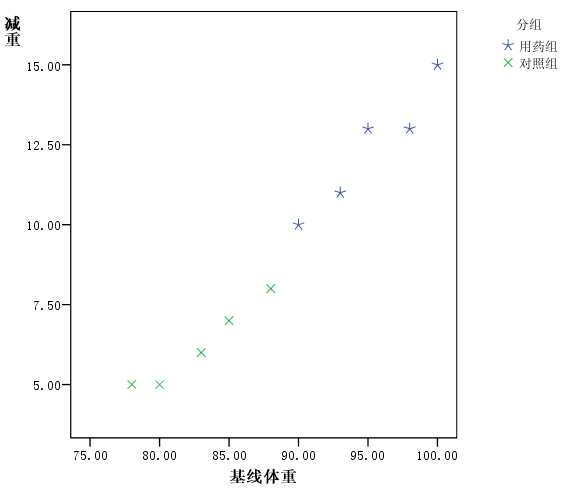
\includegraphics[width=.80\linewidth]{assets/weight2014.png}\end{center}


\begin{choices}

\item 两组基线体重均衡

\item 基线体重与用药存在交互作用

\item 基线体重与减重的分组回归线平行且重合

\item 成组比较(减重) 结果为两组差异无统计学意义

\item 减肥药有效

\end{choices}

\end{minipage}\par\vspace{4pt}

\par\addvspace{6pt}\noindent\begin{minipage}{\linewidth}

\Question{E14-5}{将连续疗效二分类}

如果研究者以体重减少5kg为疗效判断指标,将结果变量设为有效和无效并使用logistic回归分析,则以下错误的说法是


\begin{choices}

\item 损失了数据信息,降低了检验效能

\item 如果发现药物有效,同时也可确定药物的临床使用价值

\item 如果没有其他混杂因素,可以同时计算 RR和OR

\item 可以用有效和无效分组,比较两组人的平均体重,如果有效组平均体重高于无效组,则说明减肥药对胖人有效

\item 可以考察基线体重和分组变量间的交互作用

\end{choices}

\end{minipage}\par\vspace{4pt}

\Needspace{7\baselineskip}\subsubsection*{共用资料：两所医院的护理量与新生儿死亡}

医院和护理按表中1/2编码，响应为死亡1、存活0。下表给出4个Logistic模型的原输出；P显示0.000表示小于显示精度，不代表概率严格为0。

\begin{center}\small\setlength{\tabcolsep}{3.5pt}\renewcommand{\arraystretch}{1.18}\begin{tabular}{@{}lrrrr@{}}
\toprule
医院 & 护理量 & 死亡 & 存活 & 死亡率\% \\
\midrule

A（1） & 少（1） & 3 & 176 & 1.676 \\
A（1） & 多（2） & 4 & 293 & 1.347 \\
B（2） & 少（1） & 17 & 197 & 7.944 \\
B（2） & 多（2） & 1 & 23 & 4.0 \\
\bottomrule\end{tabular}\end{center}

\begin{center}\small\setlength{\tabcolsep}{3.5pt}\renewcommand{\arraystretch}{1.18}\begin{tabular}{@{}lrrrrrrr@{}}
\toprule
模型 & 变量 & B & SE & Wald & df & P & Exp(B) \\
\midrule

1 & hospital & 2.085 & 1.705 & 1.495 & 1 & 0.221 & 8.048 \\
1 & nurse & 0.241 & 1.865 & 0.017 & 1 & 0.897 & 1.273 \\
1 & hospital×nurse & -0.463 & 1.304 & 0.126 & 1 & 0.722 & 0.629 \\
1 & 截距 & -5.935 & 2.782 & 4.553 & 1 & 0.033 & 0.003 \\
2 & hospital & 1.507 & 0.528 & 8.159 & 1 & 0.004 & 4.515 \\
2 & nurse & -0.395 & 0.592 & 0.445 & 1 & 0.505 & 0.674 \\
2 & 截距 & -5.089 & 1.423 & 12.78 & 1 & 0.0 & 0.006 \\
3 & hospital & 1.701 & 0.453 & 14.115 & 1 & 0.0 & 5.482 \\
3 & 截距 & -5.906 & 0.8 & 54.499 & 1 & 0.0 & 0.003 \\
4 & nurse & -1.22 & 0.506 & 5.822 & 1 & 0.016 & 0.295 \\
4 & 截距 & -1.705 & 0.643 & 7.027 & 1 & 0.008 & 0.182 \\
\bottomrule\end{tabular}\end{center}


\par\addvspace{6pt}\noindent\begin{minipage}{\linewidth}

\Question{E14-6}{护理量与医院的调整分析}

根据统计结果,新生儿死亡的影响因素是


\begin{choices}

\item 仅医院原因

\item 仅护理量原因

\item 医院原因和护理量二者均是影响因素

\item 不同护理量下,A,B医院的影响不同

\item 无法判断

\end{choices}

\end{minipage}\par\vspace{4pt}

\par\addvspace{6pt}\noindent\begin{minipage}{\linewidth}

\Question{E14-7}{未调整的护理OR}

如果忽略医院不同的影响做单因素分析,较高护理量对较低护理量的OR是


\begin{choices}

\item 0

\item 0.295

\item 0.674

\item 1

\item 1.273

\end{choices}

\end{minipage}\par\vspace{4pt}

\par\addvspace{6pt}\noindent\begin{minipage}{\linewidth}

\Question{E14-8}{最终医院OR}

根据最终统计结果,B医院对A医院的OR是


\begin{choices}

\item 0

\item 1

\item 4.5

\item 5.5

\item 8.0

\end{choices}

\end{minipage}\par\vspace{4pt}

\par\addvspace{6pt}\noindent\begin{minipage}{\linewidth}

\Question{E14-9}{被删除项的模型OR}

根据最终统计结果,较高护理量对较低护理量的OR是


\begin{choices}

\item 0

\item 0.295

\item 0.674

\item 1

\item 1.273

\end{choices}

\end{minipage}\par\vspace{4pt}

\par\addvspace{6pt}\noindent\begin{minipage}{\linewidth}

\Question{E14-10}{医院间的风险比}

根据最终统计结果,B医院对A医院的RR是


\begin{choices}

\item 1.1

\item 4.5

\item 5.1

\item 5.5

\item 8.0

\end{choices}

\end{minipage}\par\vspace{4pt}

\par\addvspace{6pt}\noindent\begin{minipage}{\linewidth}

\Question{E14-11}{三个OR的组合}

某药效临床试验,研究对象分低龄和高龄两组随机分配入用药组和安慰剂组,使用logistic model,以高龄和安慰剂为参照,得到年龄的OR=2,药物的OR=5,年龄和药物的交互作用为0.8,则低龄用药组对高龄安慰剂组的OR是


\begin{choices}

\item 6.2

\item 7.8

\item 8

\item 10

\item 10.8

\end{choices}

\end{minipage}\par\vspace{4pt}

\par\addvspace{6pt}\noindent\begin{minipage}{\linewidth}

\Question{E14-13}{一般线性模型与参照类别}

关于GLM,以下判断正确的是


\begin{choices}

\item 不要求因变量服从正态分布

\item 要求自变量互相独立

\item 对于有交互作用的模型,可以在估计交互作用后评价主效应

\item 对于无交互作用模型,可以直接做单因素方差分析

\item 可以任意指定某分类变量中某类的主效应参数(回归系数)为0

\end{choices}

\end{minipage}\par\vspace{4pt}

\Needspace{7\baselineskip}\subsubsection*{共用资料：旧题文献2与Framingham模型}

原题引用《多元线性回归\ldots\ldots》及Framingham心脏病研究的表1、方程；该原文未随本题库提供。现有``生命质量影响因素''是另一篇2018年文献，不能代替。以下保留原题，涉及具体数值与文章原句的答案须等待原文核验。


\par\addvspace{6pt}\noindent\begin{minipage}{\linewidth}

\Question{E14-18}{由原文方程计算风险}

根据表1结果,45岁,女性,SBP\textless22kPa,其冠心病发病的概率是


\begin{choices}

\item 0.0613

\item 0.0277

\item 0.1273

\item 0.1680

\item 尚无法判断

\end{choices}

\end{minipage}\par\vspace{4pt}

\Needspace{7\baselineskip}\subsubsection*{共用资料：BMI与非吸烟女性肺癌}

上海市肿瘤登记收集1992年2月1日至1993年底的女性肺癌新病例649例，年龄35---69岁；73\%由病理或细胞学确诊，其余经胸部影像。按病例年龄分布，以5岁为组作频数匹配，在市区人群中随机抽取健康对照675例。非吸烟病例、对照分别为504、601例。对非吸烟者拟合多变量非条件Logistic模型，调整烹调油烟、用油类型、被动吸烟、饮茶、肺结核、家族史、月经生育等因素；下表为两个调整层次的结果。原结论：``体质指数可能是非吸烟女性肺癌的危险因素之一。''

\begin{center}\small\setlength{\tabcolsep}{3.5pt}\renewcommand{\arraystretch}{1.18}\begin{tabular}{@{}lrrrrr@{}}
\toprule
BMI组 & 病例/对照 & ORI & 95\% CII & ORII & 95\% CIII \\
\midrule

\(\ge\) 25.15 & 94/152 & 1 & --- & 1 & --- \\
22.86---25.14 & 103/159 & 1.017 & 0.706---1.464 & 1.021 & 0.707---1.473 \\
20.96---22.85 & 129/140 & 1.399 & 0.976---2.006 & 1.498 & 0.971---2.012 \\
\textless20.96 & 176/150 & 1.793 & 1.268---2.536 & 1.794 & 1.263---2.548 \\
\bottomrule\end{tabular}\end{center}

两个模型的趋势检验均报告 \(P=0.0002\)。


\par\addvspace{6pt}\noindent\begin{minipage}{\linewidth}

\Question{E14-22}{病例对照设计}

本研究属于


\begin{choices}

\item 横断面调查研究

\item 病例对照研究

\item 队列研究

\item 社区干预研究

\item 随机对照临床试验

\end{choices}

\end{minipage}\par\vspace{4pt}

\par\addvspace{6pt}\noindent\begin{minipage}{\linewidth}

\Question{E14-23}{病例对照研究的实施难点}

按此研究设计,在操作上最难做到的是


\begin{choices}

\item 获得癌症病人资料

\item 获得对照组人群资料

\item 问卷调查

\item BMI测试

\item 统计分析

\end{choices}

\end{minipage}\par\vspace{4pt}

\par\addvspace{6pt}\noindent\begin{minipage}{\linewidth}

\Question{E14-24}{表内数字核查}

此研究中肯定存在的问题有


\begin{choices}

\item 统计数字有误

\item 假设检验有误

\item OR计算有误

\item 资料获取方法有误

\item 模型选择有误

\end{choices}

\end{minipage}\par\vspace{4pt}

\par\addvspace{6pt}\noindent\begin{minipage}{\linewidth}

\Question{E17-M6}{有序分类自变量的分析}

当Y为数值变量,X为有序多分类变量,则以下正确的说法是


\begin{choices}

\item 使用单因素方差分析最优

\item 可以直接进行多次t检验

\item 使用等级相关分析最优

\item 使用GLM进行分析最优

\item 如果LINE假设成立，宜用线性回归分析，模型假设检验的自由度为1。

\end{choices}

\end{minipage}\par\vspace{4pt}

\par\addvspace{6pt}\noindent\begin{minipage}{\linewidth}

\Question{E17-M19}{温度与催化剂的关系}

欲考察某化学反应条件(温度、催化剂)与底物浓度(变化)的关系,数据分析宜使用


\begin{choices}

\item 分组散点图。

\item 边际均数图。

\item 偏回归图。

\item QQ图。

\item 残差分布图。

\end{choices}

\end{minipage}\par\vspace{4pt}

\Needspace{7\baselineskip}\subsubsection*{共用资料：减肥训练与基线不均衡}

在一个减肥训练班（训练方法为控制饮食与锻炼）中招募志愿者服用减肥药，志愿者和其他人都继续饮食控制与锻炼。用试验前后体重减少量评价疗效；研究人员发现服药志愿者通常比非志愿者更肥胖，两个组的基线不均衡。


\par\addvspace{6pt}\noindent\begin{minipage}{\linewidth}

\Question{E17-C1}{基线不均衡还能否分析}

如果服药组与对照组的体重基线不均衡,则本研究


\begin{choices}

\item 无法回答药物是否有效问题

\item 使用GLM模型可以消除体重不均衡因素,回答药物是否有效问题

\item 不妨使用t 检验做成组比较

\item 在一定情况下可以回答药物是否有效问题

\item 因为没有随机入组,本试验无效

\end{choices}

\end{minipage}\par\vspace{4pt}

\par\addvspace{6pt}\noindent\begin{minipage}{\linewidth}

\Question{E17-C2}{药效依赖基线水平}

如果基线体重和分组变量存在交互作用,则


\begin{choices}

\item 可以计算标准化回归系数做进一步比较

\item 需进一步做成组设计均数比较的t检验

\item 药效大小与体重有关

\item 可以计算偏相关系数做疗效判断

\item 可以判定药物减肥有效

\end{choices}

\end{minipage}\par\vspace{4pt}

\par\addvspace{6pt}\noindent\begin{minipage}{\linewidth}

\Question{E17-C3}{共同斜率模型的下一步}

如果基线体重和分组变量不存在交互作用,则


\begin{choices}

\item 即可判定减肥药有效

\item 可以通过进一步分析得出药物是否有效的结论

\item 如果基线体重与体重减少量无线性关系,可以认为减肥药有效

\item 如果基线体重与体重减少量有线性关系,亦难评价减肥药是否有效

\item 即可做单因素方差分析来进一步判定

\end{choices}

\end{minipage}\par\vspace{4pt}

\par\addvspace{6pt}\noindent\begin{minipage}{\linewidth}

\Question{E17-C4}{重叠趋势与基线混杂}

如果下图是数据的散点图,则最可能的结论是

\begin{center}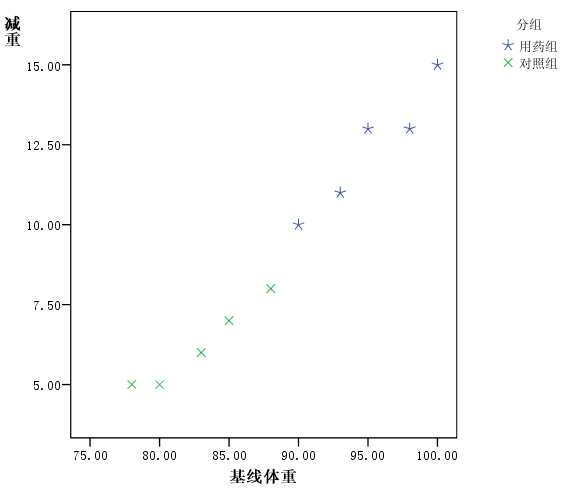
\includegraphics[width=.80\linewidth]{assets/weight2017.png}\end{center}


\begin{choices}

\item 两组基线体重均衡

\item 基线体重与分组变量存在交互作用

\item 减肥药无效

\item 基线体重与减重无线性关系

\item 成组比较(减重) 结果为两组差异无统计学意义

\end{choices}

\end{minipage}\par\vspace{4pt}

\par\addvspace{6pt}\noindent\begin{minipage}{\linewidth}

\Question{E17-C5}{基线均衡后的分析选择}

如果两组基线体重均衡,则以下错误的说法是


\begin{choices}

\item 无把握判断减肥药是否有效

\item 可以科学判断训练方法是否有效

\item 可以使用t检验

\item 必须基线体重为协变量建立GLM

\item 可以使用方差分析

\end{choices}

\end{minipage}\par\vspace{4pt}

\Needspace{7\baselineskip}\subsubsection*{共用资料：急诊就诊量与气象要素}

阅读随包的《急诊就诊量与气象要素的相关性分析》（费敏，2008）。研究分析2005---2006连续730天数据，报告急诊199649人次、日均274.5人次；7月最高、2月最低。文中写采用post hoc检验。回归从9个气象变量中筛出以下4项：

\begin{center}\small\setlength{\tabcolsep}{3.5pt}\renewcommand{\arraystretch}{1.18}\begin{tabular}{@{}lrrrr@{}}
\toprule
变量 & B & SE & 标准化\(\beta\) & P \\
\midrule

平均相对湿度 & 1.011 & 0.159 & 0.244 & \textless.001 \\
最高气温 & 1.126 & 0.546 & 0.212 & \textless.05 \\
最低气温 & 2.2 & 0.591 & 0.378 & \textless.001 \\
最大风速 & -0.606 & 0.091 & -0.207 & \textless.001 \\
\bottomrule\end{tabular}\end{center}

给出的预测公式截距为285.481。讨论中认为春节期间停工休息可能减少意外就诊，也讨论高温和低温均可能增加急症。文中未给出本模型的 \(R^2\)、时间序列残差或共线性诊断；所引用的84\%与44\%来自别人的研究。


\par\addvspace{6pt}\noindent\begin{minipage}{\linewidth}

\Question{E17-L1}{月份均数的事后比较}

7月份和2月份日平均就诊人次与其他月份相比差异有统计学意义,作者最可能使用的统计方法是


\begin{choices}

\item GLM

\item t检验

\item 线性回归

\item 方差分析后的多重比较 post-hoc

\item 非参数检验

\end{choices}

\end{minipage}\par\vspace{4pt}

\par\addvspace{6pt}\noindent\begin{minipage}{\linewidth}

\Question{E17-L5}{0.0613对应什么人群}

依照Framingham心脏病研究的回归方程,0.0613是指


\begin{choices}

\item 各自变量为均数时的发病率

\item 人群基线发病率

\item 45岁女性收缩压小于22者发病率

\item 血压正常者平均发病率

\item 61岁组平均发病率

\end{choices}

\end{minipage}\par\vspace{4pt}

\par\addvspace{6pt}\noindent\begin{minipage}{\linewidth}

\Question{E21-13}{含交互模型的自由度}

GLM的交互作用模型,自变量为一个数值变量和一个4分类变量,则模型误差的自由度是


\begin{choices}

\item n-5

\item n-6

\item n-7

\item n-8

\item n-9

\end{choices}

\end{minipage}\par\vspace{4pt}

\par\addvspace{6pt}\noindent\begin{minipage}{\linewidth}

\Question{E21-14}{R公式与层次原则}

按R公式语法，下列哪些模型符合层次原则？

I. \texttt{y\ \textasciitilde{}\ x1\ +\ x2\ +\ x3\ +\ x1*x2*x3}

\begin{enumerate}
\def\labelenumi{\Roman{enumi}.}
\setcounter{enumi}{1}
\item
  \texttt{y\ \textasciitilde{}\ x1\ +\ x2\ +\ x3\ +\ x1*x2\ +\ x2*x3\ +\ x1*x2*x3}
\item
  \texttt{y\ \textasciitilde{}\ x1\ +\ x2\ +\ x3\ +\ x1*x2*x3}
\end{enumerate}

三个公式按回忆稿原样保留（I与III相同）。


\begin{choices}

\item I

\item II

\item III

\item I\&II

\item I\&II\&III

\end{choices}

\end{minipage}\par\vspace{4pt}

\par\addvspace{6pt}\noindent\begin{minipage}{\linewidth}

\Question{E21-15}{aov的顺序平方和}

关于aov()函数,正确的说法有 I、aov()函数对交互作用的检验与自变量的顺序有关 II、aov()函数对主效应的检验与自变量的顺序有关 III、aov()函数可以用于协方差矩阵的球形检验


\begin{choices}

\item I

\item II

\item III

\item I\&II

\item I\&II\&III

\end{choices}

\end{minipage}\par\vspace{4pt}

\Needspace{7\baselineskip}\subsubsection*{共用资料：减肥训练与基线不均衡}

在一个减肥训练班（训练方法为控制饮食与锻炼）中招募志愿者服用减肥药，志愿者和其他人都继续饮食控制与锻炼。用试验前后体重减少量评价疗效；研究人员发现服药志愿者通常比非志愿者更肥胖，两个组的基线不均衡。


\par\addvspace{6pt}\noindent\begin{minipage}{\linewidth}

\Question{E21-21}{基线不均衡还能否分析}

如果服药组与对照组的体重基线不均衡,则本研究


\begin{choices}

\item 无法回答药物是否有效问题

\item 使用GLM模型可以消除体重不均衡因素,回答药物是否有效问题

\item 不妨使用t 检验做成组比较

\item 在一定情况下可以回答药物是否有效问题

\item 因为没有随机入组,本试验无效

\end{choices}

\end{minipage}\par\vspace{4pt}

\par\addvspace{6pt}\noindent\begin{minipage}{\linewidth}

\Question{E21-22}{药效依赖基线水平}

如果基线体重和分组变量存在交互作用,则


\begin{choices}

\item 可以计算标准化回归系数做进一步比较

\item 需进一步做成组设计均数比较的t检验

\item 药效大小与体重有关

\item 可以计算偏相关系数做疗效判断

\item 可以判定药物减肥有效

\end{choices}

\end{minipage}\par\vspace{4pt}

\par\addvspace{6pt}\noindent\begin{minipage}{\linewidth}

\Question{E21-23}{共同斜率模型的下一步}

如果基线体重和分组变量不存在交互作用,则


\begin{choices}

\item 即可判定减肥药有效

\item 可以通过进一步分析得出药物是否有效的结论

\item 如果基线体重与体重减少量无线性关系,可以认为减肥药有效

\item 如果基线体重与体重减少量有线性关系,亦难评价减肥药是否有效

\item 即可做单因素方差分析来进一步判定

\end{choices}

\end{minipage}\par\vspace{4pt}

\par\addvspace{6pt}\noindent\begin{minipage}{\linewidth}

\Question{E21-24}{重叠趋势与基线混杂}

如果下图是数据散点图，则最可能的结论是：

\begin{center}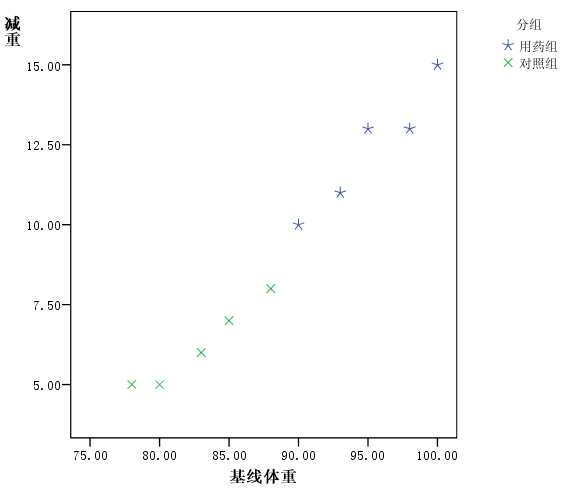
\includegraphics[width=.80\linewidth]{assets/weight2021.png}\end{center}


\begin{choices}

\item 两组基线体重均衡

\item 基线体重与分组变量存在交互作用

\item 减肥药无效

\item 基线体重与减重无线性关系

\item 成组比较(减重) 结果为两组差异无统计学意义

\end{choices}

\end{minipage}\par\vspace{4pt}

\par\addvspace{6pt}\noindent\begin{minipage}{\linewidth}

\Question{E21-25}{设计阶段的混杂控制}

这个研究给你哪些启发？

I. 只要一项基线指标均衡，就一定不存在混杂。

\begin{enumerate}
\def\labelenumi{\Roman{enumi}.}
\setcounter{enumi}{1}
\item
  组间检验不显著就证明处理完全无效。
\item
  设计阶段未考虑混杂，可能无法回答研究者关心的问题。
\end{enumerate}


\begin{choices}

\item I

\item II

\item III

\item I\&II

\item I\&II\&III

\end{choices}

\end{minipage}\par\vspace{4pt}

\par\addvspace{6pt}\noindent\begin{minipage}{\linewidth}

\Question{E21-8}{一般线性模型的组成}

一个连续结局、一个二分类因素和一个数值协变量，无交互的含截距一般线性模型可写为：


\begin{choices}

\item \(E(Y\mid X,G)=\beta_0+\beta_X X+\beta_G G\)。

\item \(Y\)必须与\(X\)相互独立。

\item 必须省略截距。

\item 必须将连续结局先二分类。

\item 无需任何关于误差和设计的条件。

\end{choices}

\end{minipage}\par\vspace{4pt}

\par\addvspace{6pt}\noindent\begin{minipage}{\linewidth}

\Question{E21-11}{交互模型的层次性}

若模型保留 \(X_1X_2\) 交互项，通常应同时保留：


\begin{choices}

\item 仅截距。

\item X1与X2两个低阶主效应。

\item 只保留P值较小的一个主效应。

\item 删除全部主效应。

\item 任意与题目无关的变量。

\end{choices}

\end{minipage}\par\vspace{4pt}

\par\addvspace{6pt}\noindent\begin{minipage}{\linewidth}

\Question{N19-14}{三分类因素的设计矩阵}

含截距、3类别因素的一元一般线性模型，满秩参数数目为：


\begin{choices}

\item 1。

\item 2。

\item 3。

\item 4。

\item n。

\end{choices}

\end{minipage}\par\vspace{4pt}

\par\addvspace{6pt}\noindent\begin{minipage}{\linewidth}

\Question{N19-15}{交互项的条件效应}

模型 \(E(Y)=b_0+b_XX+b_GG+b_{XG}XG\) 中，给定X的组1对组0均值差为：


\begin{choices}

\item \(b_G+b_{XG}X\)。

\item \(b_G\)对所有X不变。

\item \(b_X\)。

\item \(b_0\)。

\item \(b_X+b_G\)。

\end{choices}

\end{minipage}\par\vspace{4pt}

\par\addvspace{6pt}\noindent\begin{minipage}{\linewidth}

\Question{N19-16}{中心化协变量}

将数值协变量减去一个常数重新拟合同一可等价表达的含交互模型，通常：


\begin{choices}

\item 拟合值可保持相同，但截距及部分主效应解释改变。

\item 所有P值都必变为0。

\item 必须删去交互项。

\item 所有观测的Y值改变。

\item 残差必增大。

\end{choices}

\end{minipage}\par\vspace{4pt}

\par\addvspace{6pt}\noindent\begin{minipage}{\linewidth}

\Question{N19-17}{非平衡设计中的顺序平方和}

非平衡资料的I型平方和一般：


\begin{choices}

\item 可能依赖模型项加入顺序。

\item 与顺序永远无关。

\item 总等于III型平方和。

\item 无需考虑交互结构。

\item 只适用于二分类结局。

\end{choices}

\end{minipage}\par\vspace{4pt}

\par\addvspace{6pt}\noindent\begin{minipage}{\linewidth}

\Question{N19-18}{改变参照类别}

在同一满秩模型空间内改变分类变量的参照组，通常：


\begin{choices}

\item 拟合值与整体模型检验不变，系数含义改变。

\item 预测值一定改变。

\item 变量类型由分类变连续。

\item 样本量增加。

\item 所有系数均不变。

\end{choices}

\end{minipage}\par\vspace{4pt}

\par\addvspace{6pt}\noindent\begin{minipage}{\linewidth}

\Question{N19-25}{肿瘤类型的编码}

若把胶质瘤、脑膜瘤、垂体瘤作为无序3分类解释变量，含截距时通常需要：


\begin{choices}

\item 2个哑变量。

\item 直接用1、2、3且不加任何间距假定。

\item 3个哑变量加截距且声称满秩。

\item 不需要任何变量。

\item 先将结局二分类。

\end{choices}

\end{minipage}\par\vspace{4pt}

\subsection{简答题}

\Needspace{7\baselineskip}\subsubsection*{共用资料：BMI与非吸烟女性肺癌}

上海市肿瘤登记收集1992年2月1日至1993年底的女性肺癌新病例649例，年龄35---69岁；73\%由病理或细胞学确诊，其余经胸部影像。按病例年龄分布，以5岁为组作频数匹配，在市区人群中随机抽取健康对照675例。非吸烟病例、对照分别为504、601例。对非吸烟者拟合多变量非条件Logistic模型，调整烹调油烟、用油类型、被动吸烟、饮茶、肺结核、家族史、月经生育等因素；下表为两个调整层次的结果。原结论：``体质指数可能是非吸烟女性肺癌的危险因素之一。''

\begin{center}\small\setlength{\tabcolsep}{3.5pt}\renewcommand{\arraystretch}{1.18}\begin{tabular}{@{}lrrrrr@{}}
\toprule
BMI组 & 病例/对照 & ORI & 95\% CII & ORII & 95\% CIII \\
\midrule

\(\ge\) 25.15 & 94/152 & 1 & --- & 1 & --- \\
22.86---25.14 & 103/159 & 1.017 & 0.706---1.464 & 1.021 & 0.707---1.473 \\
20.96---22.85 & 129/140 & 1.399 & 0.976---2.006 & 1.498 & 0.971---2.012 \\
\textless20.96 & 176/150 & 1.793 & 1.268---2.536 & 1.794 & 1.263---2.548 \\
\bottomrule\end{tabular}\end{center}

两个模型的趋势检验均报告 \(P=0.0002\)。


\par\addvspace{6pt}\noindent\begin{minipage}{\linewidth}

\Question{E14-25}{一句话评价肺癌研究}

请用一句话对此研究结论作评价。


\worklines{3}

\end{minipage}\par\vspace{4pt}

\par\addvspace{6pt}\noindent\begin{minipage}{\linewidth}

\Question{S20-3}{一般线性模型的层次规则}

简述一般线性模型建模的层次规则。


\worklines{3}

\end{minipage}\par\vspace{4pt}

\par\addvspace{6pt}\noindent\begin{minipage}{\linewidth}

\Question{S20-4}{从一般线性模型看常用分析}

从一般线性模型的简化形式，总结数值结局的常见统计分析方法。


\worklines{3}

\end{minipage}\par\vspace{4pt}

\subsection{计算与分析题}

\par\addvspace{6pt}\noindent\begin{minipage}{\linewidth}

\Question{C20-3}{儿童测验：组别、年龄与交互}

data3为儿童生长发育测验分数，分两个有害因素暴露组和一个对照组，以年龄为协变量，用一般线性模型分析： 1. 按步骤筛选最终模型。 2. 给出最终模型方差分析表。 3. 给出回归方程，以对照为参照组。 4. 作统计学和专业解释。

原儿童测验文件没有附上。2023 data3标注为BMR，不能不加说明地当作儿童测验原数据。


\worklines{3}

\end{minipage}\par\vspace{4pt}

\par\addvspace{6pt}\noindent\begin{minipage}{\linewidth}

\Question{C21-3}{儿童测验：组别、年龄与交互}

data3为儿童生长发育测验分数，分两个有害因素暴露组和一个对照组，以年龄为协变量，用一般线性模型分析： 1. 按步骤筛选最终模型。 2. 给出最终模型方差分析表。 3. 给出回归方程，以对照为参照组。 4. 作统计学和专业解释。

原儿童测验文件没有附上。2023 data3标注为BMR，不能不加说明地当作儿童测验原数据。


\worklines{3}

\end{minipage}\par\vspace{4pt}



\clearpage\section{补充练习}

本节为配合正文新编的补充练习，按题型排列，题号接续本章往年题，解析见章末。

\subsection{单项选择题}

\par\addvspace{6pt}\noindent\begin{minipage}{\linewidth}

\Question{X26-3-1}{小鼠饮食试验的参照编码}

正文小鼠饮食试验中，NR、HSP、HPP三组各10只，体重变化均数依次为5.436、2.781、3.956 g。以NR为参照，\(D_H,D_P\) 分别表示HSP、HPP组，模型为 \(\hat Y=b_0+b_HD_H+b_PD_P\)。以下说法正确的是：


\begin{choices}

\item 截距必为三组合并均数4.0577。

\item \(b_H=2.781,\,b_P=3.956\)。

\item 组别整体检验的分子自由度为3。

\item \(b_0=5.436,\,b_H=-2.655,\,b_P=-1.480\)。

\item 因每只小鼠有干预前后体重，这个变化值模型必须另加入时间项。

\end{choices}

\end{minipage}\par\vspace{4pt}

\par\addvspace{6pt}\noindent\begin{minipage}{\linewidth}

\Question{X26-3-2}{随机区组设计的误差自由度}

正文软骨修复试验设8窝兔，每窝3只，在每窝内分别随机安排3种处理，每个``窝别×处理''组合只有1只兔。按正文的无交互随机区组模型分析，以下说法正确的是：


\begin{choices}

\item 处理效应以 \(F(2,21)\) 检验，因为共有24只兔。

\item 处理效应以 \(F(2,14)\) 检验，模型不单独估计窝别×处理交互。

\item 可用剩余14个自由度同时独立估计交互和随机误差。

\item 窝别和处理自由度分别为8和3。

\item 每窝有3只兔，因此属于三时点重复测量。

\end{choices}

\end{minipage}\par\vspace{4pt}

\Question{X26-3-3}{顺序平方和的数值辨析}

同一样本中，X是数值协变量，G是分类因素。四个含截距模型的残差平方和如下，且 \(Y\sim X+G\) 不含交互：

\begin{center}\small\setlength{\tabcolsep}{5pt}\renewcommand{\arraystretch}{1.18}\begin{tabular}{@{}lllll@{}}
\toprule
模型 & 仅截距 & X & G & X+G \\
\midrule

残差平方和 & 100 & 70 & 85 & 60 \\
\bottomrule\end{tabular}\end{center}

采用I型平方和时，以下说法正确的是：


\begin{choices}

\item 先放X后放G，G的顺序平方和为10；先放G后放X，X的顺序平方和为25。

\item 两种顺序下，G的平方和均为15。

\item 改变顺序后，最终模型残差平方和必改变。

\item 先放X时，G的顺序平方和为40。

\item 两种顺序下，X与G的顺序平方和之和不同。

\end{choices}

\subsection{简答题}

\par\addvspace{6pt}\noindent\begin{minipage}{\linewidth}

\Question{X26-3-4}{胆固醇协方差分析的结果解释}

正文比较正常体重组和超重组的胆固醇，年龄为X，正常组 \(G=0\)、超重组 \(G=1\)。年龄×组别交互的 \(P=0.935\)；删去交互后的拟合式为 \[\hat Y=0.760534+0.094169X+0.895493G.\] 在共同年龄50.23岁处，模型给出的修正均数约为5.491、6.386；组差检验 \(P=0.038\)。

按0.05水平，说明采用哪种模型、修正均数比较的含义，以及能否据``交互不显著''把两组直接合为一条直线。


\worklines{3}

\end{minipage}\par\vspace{4pt}

\subsection{计算与分析题}

\Question{X26-3-5}{两药析因试验的交互填空}

正文例3将12名缺铁性贫血患者分为4组，每组3人，一个月后红细胞增加数如下（单位沿用正文：百万/mm\(^3\)）：

\begin{center}\small\setlength{\tabcolsep}{5pt}\renewcommand{\arraystretch}{1.18}\begin{tabular}{@{}lll@{}}
\toprule
甲药A & 乙药B & 3名患者的增加数 \\
\midrule

不用 & 不用 & 0.8，0.9，0.7 \\
用 & 不用 & 1.3，1.2，1.1 \\
不用 & 用 & 0.9，1.1，1.0 \\
用 & 用 & 2.1，2.2，2.0 \\
\bottomrule\end{tabular}\end{center}

\begin{enumerate}
\def\labelenumi{\arabic{enumi}.}
\tightlist
\item
  以不用药为0、用药为1，写出含交互的回归方程 \(\hat Y=b_0+b_AA+b_BB+b_{AB}AB\)。
\item
  填写A、B、A×B、误差的平方和、自由度、均方与F值。
\item
  已知 \(F_{0.95}(1,8)=5.318\)，检验交互作用；计算不用乙药和用乙药时甲药效应的估计，并说明为何不能只用一个甲药效应概括。
\item
  在本题平衡设计中，以正文的和为零约束 \(\sum\alpha_i=\sum\beta_j=0\) 表示效应时，交互效应四个格子的估计是多少？它们与0/1编码的 \(b_{AB}\) 是否为同一个参数？
\end{enumerate}


\worklines{3}

\clearpage\section{习题解析}

\begin{keyidea}[核对方式]题号与前文一一对应。补写范围、原题歧义及数据还原方法列在相应答案中。\end{keyidea}

\Answer{E14-1}{调整不均衡的基线}

\textbf{答案：D（一般线性模型/协方差分析）。}

以减重为结局，纳入基线体重、分组及必要的交互项。数值协变量加分类因素可用一般线性模型表示。C若指含哑变量的多重线性回归，也能表达同一模型，故选项术语有重叠；D是课程意图。调整不能自动消除未测混杂。


\Answer{E14-2}{基线与处理的交互}

\textbf{答案：A（仅就统一药效的解释而言）。}

交互意味着药效与基线体重有关，应解释 \(\beta_G+\beta_{GX}X\) 或报告不同基线水平的简单效应。不能再只用一个恒定药效概括。A若被理解为完全无法评价药效则过强；其余选项也不是正确替代交互分析的方法。


\Answer{E14-3}{无交互后的疗效评价}

\textbf{答案：B。}

未发现交互可进一步用共同斜率ANCOVA评价调整后的组差；若协变量与结局的关系也可忽略，再考虑简化。无交互本身既不证明有效，也不证明无效。


\Answer{E14-4}{散点图与表观药效}

\textbf{答案：C（示意图的命题意图）。}

图中两组分布在不同基线区间，整体大致沿同一趋势；未经调整的减重差可能来自基线。它不能证明疗效，且基线区间缺乏重叠，调整高度依赖模型外推。示意图也不足以正式证明两条线完全平行重合，应以模型与不确定性为准。


\Answer{E14-5}{将连续疗效二分类}

\textbf{答案：D最直接；B也表述过强。}

按疗效分组再比较基线体重不能替代处理效应或处理×基线交互分析，故D的推论不成立。B也不能仅凭统计结果就确定综合临床使用价值，还需收益、伤害等证据。二分类通常损失信息；随访设计和分母合适时可分别估计RR与OR，但两者不是同一量。


\Answer{E14-6}{护理量与医院的调整分析}

\textbf{答案：A（统计关联层面）。}

交互项P=.722，护理在调整医院后P=.505；按原卷逐步简化口径仅医院项留下。这里是统计关联，不能称为已证明``医院原因''导致死亡。


\Answer{E14-7}{未调整的护理OR}

\textbf{答案：B。}

单因素护理模型的指数系数为 \(e^{-1.220}\approx0.295\)，也可由合并2×2表计算。该粗OR受医院构成差异影响。


\Answer{E14-8}{最终医院OR}

\textbf{答案：D。}

若``最终模型''指删除护理后的表3，\(OR=e^{1.701}\approx5.482\)，选5.5。若保留护理调整，则表2为4.515，须区别模型。


\Answer{E14-9}{被删除项的模型OR}

\textbf{答案：D（简化模型所施加的约束）。}

只含医院的模型将护理系数设为0，故模型内 \(OR=e^0=1\)；这不是证明真实护理效应等于0。若问表2的调整OR则为0.674。


\Answer{E14-10}{医院间的风险比}

\textbf{答案：C。}

两院死亡风险为 \(7/476\) 与 \(18/238\)，因此 \(RR=(18/238)/(7/476)=5.1429\)。它不同于优势比约5.482。


\Answer{E14-11}{三个OR的组合}

\textbf{答案：C。}

把题中0.8理解为交互项的OR，则低龄且用药相对于高龄且安慰剂的OR为 \(2\times5\times0.8=8\)。若0.8指对数系数，结果应为 \(2\times5e^{0.8}\)；原选项支持前一种解释。


\Answer{E14-13}{一般线性模型与参照类别}

\textbf{答案：E（参照编码）。}

这里GLM指一般线性模型。可选任一类别为参照并将对应冗余参数设为0，需保持整套编码一致。有交互时仍可解释特定参照条件下的主效应系数，但不能忽略交互作无条件解释，因此C措辞也存在歧义。


\Answer{E14-18}{由原文方程计算风险}

\textbf{答案：原文缺失，不能确认原题选项。}

需要表1完整系数、变量定义、参照及连接函数。如果是Logistic，应先求线性预测子，再作 \(p=1/(1+e^{-\eta})\)；如文中给的是线性概率模型，计算和适用边界不同。这里不能因附件缺失就冒认原考试正确项为E。


\Answer{E14-22}{病例对照设计}

\textbf{答案：B。}

先按是否为肺癌病例抽取病例与健康对照，再比较BMI和其他特征，是病例对照研究；对照按年龄分布频数匹配。


\Answer{E14-23}{病例对照研究的实施难点}

\textbf{答案：B（通常的命题意图）。}

对照必须来自与病例相同的来源人群，并能代表产生病例的暴露分布，选择和获取合适对照通常最困难。BMI测量时点也很重要，病后体重变化可能带来反向因果；``最难''不是普遍定理。


\Answer{E14-24}{表内数字核查}

\textbf{答案：A。}

表中病例数 \(94+103+129+176=502\)，与正文非吸烟病例504不符；对照数相加为601。可指出计数不一致，但仅凭摘要不能判定是遗漏、排除未说明还是排版错误。


\Answer{E17-M6}{有序分类自变量的分析}

\textbf{答案：E需附加线性评分假定；否则D。}

若把有序水平编码为有实际意义的数值，且条件均值对这一分数确为直线，可用1个斜率，自由度1。只有顺序而间距未知时，不应自动如此，可用分类因子GLM或预设有序对比。原题条件不足，不能无条件称某法``最优''。


\Answer{E17-M19}{温度与催化剂的关系}

\textbf{答案：A。}

按催化剂组画温度与结局的散点及拟合线，有助于检查组间斜率差异和非线性。


\Answer{E17-C1}{基线不均衡还能否分析}

\textbf{答案：D。}

非随机和基线不均衡增加混杂风险，但不使研究完全无效。在协变量测量充分、模型形式合适、组间有可比范围等条件下可估计调整关联；不能保证一个GLM就消除了全部混杂。


\Answer{E17-C2}{药效依赖基线水平}

\textbf{答案：C。}

交互项表示分组效应随基线改变：\(\Delta(X)=\beta_G+\beta_{GX}X\)。应报告有意义基线水平下的效应与置信区间，不能从交互存在就判定整体有效。


\Answer{E17-C3}{共同斜率模型的下一步}

\textbf{答案：B。}

无交互后可进一步考察协变量及调整后的组差；是否有效仍需估计、区间和专业解释，不由``无交互''直接决定。


\Answer{E17-C4}{重叠趋势与基线混杂}

\textbf{答案：C是图示原意，但不能证明等效。}

图示中两组整体沿相似趋势，未经调整的均数差可能主要来自基线体重。C应理解为没有充分的独立药效证据，而不是从一幅图证明药物无效；基线范围缺乏重叠使任何调整依赖外推。


\Answer{E17-C5}{基线均衡后的分析选择}

\textbf{答案：D最直接；B的因果表述也过强。}

基线均衡不意味着必须用该变量作协变量；t检验、方差分析或调整模型各有合适情境。两组均接受训练而无不训练对照，仅作自身前后比较也不能严格确证训练的因果效果。


\Answer{E17-L1}{月份均数的事后比较}

\textbf{答案：D。}

附文献统计方法明确写post hoc，指总体组间比较后作多重比较；不能把每对月份未校正的t检验当成等价操作。


\Answer{E17-L5}{0.0613对应什么人群}

\textbf{答案：待原文方程与编码核实。}

概率是否对应基准人群、某年龄女性或均值协变量，取决于截距、变量中心化、哑变量和连接函数，不能只凭这个数值或研究名称推断。


\Answer{E21-13}{含交互模型的自由度}

\textbf{答案：D。}

一个四分类因素需3个哑变量，加截距1个、数值斜率1个及3个交互斜率，共8个独立参数；满秩时误差自由度为 \(n-8\)。


\Answer{E21-14}{R公式与层次原则}

\textbf{答案：E（按R公式的星号语法）。}

在R公式中 \texttt{x1*x2*x3} 会展开主效应、全部二阶交互和三阶交互；重复项会去重。因此原稿所列三个公式均包含完整层次结构。若把星号仅理解为数学乘积，结论会不同；应使用 \texttt{:} 明确表示单独交互项，避免把两种语义混用。


\Answer{E21-15}{aov的顺序平方和}

\textbf{答案：D（一般情形）；单一完整最高阶交互可有例外。}

aov常规输出使用顺序平方和。非平衡且有多个相关项时，主效应和交互项的顺序都可能影响检验；若只有一个交互且它排在所有低阶项之后，交换主效应顺序通常不改变该交互检验。III错误：aov本身不是球形检验函数。原稿对I的一概否定过于绝对。


\Answer{E21-21}{基线不均衡还能否分析}

\textbf{答案：D。}

非随机和基线不均衡增加混杂风险，但不使研究完全无效。在协变量测量充分、模型形式合适、组间有可比范围等条件下可估计调整关联；不能保证一个GLM就消除了全部混杂。


\Answer{E21-22}{药效依赖基线水平}

\textbf{答案：C。}

交互项表示分组效应随基线改变：\(\Delta(X)=\beta_G+\beta_{GX}X\)。应报告有意义基线水平下的效应与置信区间，不能从交互存在就判定整体有效。


\Answer{E21-23}{共同斜率模型的下一步}

\textbf{答案：B。}

无交互后可进一步考察协变量及调整后的组差；是否有效仍需估计、区间和专业解释，不由``无交互''直接决定。


\Answer{E21-24}{重叠趋势与基线混杂}

\textbf{答案：C是图示原意，但不能证明等效。}

图示中两组整体沿相似趋势，未经调整的均数差可能主要来自基线体重。C应理解为没有充分的独立药效证据，而不是从一幅图证明药物无效；基线范围缺乏重叠使任何调整依赖外推。


\Answer{E21-25}{设计阶段的混杂控制}

\textbf{答案：C。}

在设计阶段未保证可比性和充分测量混杂因素，事后模型可能无法回答原本关心的因果问题。基线均衡不保证所有混杂消失，无统计学差异也不能直接证明无效。


\textbf{补写说明。} 原稿只完整记录III；I、II根据主题补写，以形成可作答的题目。


\Answer{E21-8}{一般线性模型的组成}

\textbf{答案：A。}

GLM在这里指一般线性模型，用线性预测子描述条件均值，可同时纳入分类因素和数值协变量。


\textbf{补写说明。} 原第8题只记录``GLM''，本题按该主题补写。


\Answer{E21-11}{交互模型的层次性}

\textbf{答案：B。}

层次原则保留构成交互的低阶项，使参数解释和重新编码更一致；不单靠主效应P值删除它们。


\textbf{补写说明。} 原第11题整题未记录，本题新编。


\Answer{N19-14}{三分类因素的设计矩阵}

\textbf{答案：C。}

1个截距与2个哑变量，共3个类别均值的自由参数。


\textbf{补写说明。} 2019回忆稿只给出30道选择的总数及大致范围，没有记录本题原文；本题是依课程内容与所附材料新编的补充练习，不冒作恢复的原试卷。


\Answer{N19-15}{交互项的条件效应}

\textbf{答案：A。}

交互使组差随X变化，应在有数据支持的X范围内解释。


\textbf{补写说明。} 2019回忆稿只给出30道选择的总数及大致范围，没有记录本题原文；本题是依课程内容与所附材料新编的补充练习，不冒作恢复的原试卷。


\Answer{N19-16}{中心化协变量}

\textbf{答案：A。}

中心化是在同一模型空间中重参数化，可让某些主效应对应更有意义的参照值。


\textbf{补写说明。} 2019回忆稿只给出30道选择的总数及大致范围，没有记录本题原文；本题是依课程内容与所附材料新编的补充练习，不冒作恢复的原试卷。


\Answer{N19-17}{非平衡设计中的顺序平方和}

\textbf{答案：A。}

应事先说明研究假设与平方和类型；不能把不同软件默认值当作同一检验。


\textbf{补写说明。} 2019回忆稿只给出30道选择的总数及大致范围，没有记录本题原文；本题是依课程内容与所附材料新编的补充练习，不冒作恢复的原试卷。


\Answer{N19-18}{改变参照类别}

\textbf{答案：A。}

单个参数的比较对象发生变化，整体拟合模型并未改变。


\textbf{补写说明。} 2019回忆稿只给出30道选择的总数及大致范围，没有记录本题原文；本题是依课程内容与所附材料新编的补充练习，不冒作恢复的原试卷。


\Answer{N19-25}{肿瘤类型的编码}

\textbf{答案：A。}

以一个类型为参照，2个哑变量允许任意三个类别均值；用1、2、3施加了不适合无序类别的线性间距约束。


\textbf{补写说明。} 2019回忆稿只给出30道选择的总数及大致范围，没有记录本题原文；本题是依课程内容与所附材料新编的补充练习，不冒作恢复的原试卷。


\Answer{E14-25}{一句话评价肺癌研究}

\textbf{答案：参考作答。}

在所调查的非吸烟女性中，较低BMI与肺癌患病优势较高相关，但该病例对照设计不能单凭此结果确立因果关系。原稿``配对就必须用条件Logistic''的批注不准确：频数匹配可用非条件Logistic并适当调整匹配因素，不能与个体配对混同。


\Answer{S20-3}{一般线性模型的层次规则}

保留高阶交互时，通常同时保留构成它的所有低阶交互和主效应。例如含 \(A:B:C\) 时，保留A、B、C、A:B、A:C、B:C。筛选应从高阶项开始，并结合研究设计与专业意义；即使某个低阶项的单独P值较大，也不直接删去。含交互时，应解释条件效应及有意义水平下的比较。


\Answer{S20-4}{从一般线性模型看常用分析}

\begin{center}\small\setlength{\tabcolsep}{3.5pt}\renewcommand{\arraystretch}{1.18}\begin{tabular}{@{}lr@{}}
\toprule
模型形式 & 对应分析 \\
\midrule

\(Y\sim1\) & 均值估计与单样本t \\
\(Y\sim G\)，G两类 & 独立两样本t的等方差形式 \\
\(Y\sim G\)，G多类 & 单因素方差分析 \\
\(Y\sim X\) & 一元线性回归 \\
\(Y\sim X_1+\cdots+X_p\) & 多重线性回归 \\
\(Y\sim X+G\) & 共同斜率协方差分析 \\
\(Y\sim X*G\) & 不同组斜率/交互模型 \\
\(Y\sim A*B\) & 析因方差分析 \\
\bottomrule\end{tabular}\end{center}

配对t可以对个体差值作单样本t；重复测量应引入个体层次或相关误差结构，不能仅把所有观测拼入一个独立误差GLM。以上形式相通不代表它们无需各自的前提条件。


\Answer{C20-3}{儿童测验：组别、年龄与交互}

先核对对照组编码并设为参照，拟合完整 \(Y\sim age*group\)，检验年龄×组别交互；有交互则保留全部低阶项并解释不同年龄下的组差，无交互证据时比较共同斜率模型，再评估年龄和组别。

令对照的两哑变量均为0，完整模型为 \[\begin{aligned}E(Y\mid a,G)={}&\beta_0+\beta_a a+\beta_2D_2+\beta_3D_3\\&+\gamma_2aD_2+\gamma_3aD_3.\end{aligned}\] 无交互模型令两项 \(\gamma\) 为0。方差分析应说明采用嵌套模型F检验或适当的II/III型平方和；交互存在时，主效应是指定参照年龄/组别下的条件效应。

\textbf{可运行的同型演示。} 附件BMR数据把第1组暂作参照：交互F约0.161，P=.854，无明显交互；其具体最终共同斜率系数和方差分析见随包``BMR演示''输出。这些数值不代替缺失的儿童原卷答案。实际儿童解释必须结合评分方向、年龄范围、暴露定义及置信区间，不能直接推断有害暴露的因果效应。


\Answer{C21-3}{儿童测验：组别、年龄与交互}

先核对对照组编码并设为参照，拟合完整 \(Y\sim age*group\)，检验年龄×组别交互；有交互则保留全部低阶项并解释不同年龄下的组差，无交互证据时比较共同斜率模型，再评估年龄和组别。

令对照的两哑变量均为0，完整模型为 \[\begin{aligned}E(Y\mid a,G)={}&\beta_0+\beta_a a+\beta_2D_2+\beta_3D_3\\&+\gamma_2aD_2+\gamma_3aD_3.\end{aligned}\] 无交互模型令两项 \(\gamma\) 为0。方差分析应说明采用嵌套模型F检验或适当的II/III型平方和；交互存在时，主效应是指定参照年龄/组别下的条件效应。

\textbf{可运行的同型演示。} 附件BMR数据把第1组暂作参照：交互F约0.161，P=.854，无明显交互；其具体最终共同斜率系数和方差分析见随包``BMR演示''输出。这些数值不代替缺失的儿童原卷答案。实际儿童解释必须结合评分方向、年龄范围、暴露定义及置信区间，不能直接推断有害暴露的因果效应。

\clearpage\subsection*{补充练习解析}

以下为补充练习的解析。这些题目为配合正文新编，并非往年试题；题中设定的数值仅供练习。

\Answer{X26-3-1}{小鼠饮食试验的参照编码}

\textbf{答案：D。}

\(b_0=5.436\) 是NR组均数，\(b_H=2.781-5.436=-2.655\)，\(b_P=3.956-5.436=-1.480\)。检验三组总体均数相等对应联合假设 \(b_H=b_P=0\)，分子自由度2、分母自由度 \(30-3=27\)。参照组的截距不是三组合并均数。




\Answer{X26-3-2}{随机区组设计的误差自由度}

\textbf{答案：B。}

处理自由度 \(3-1=2\)，区组自由度 \(8-1=7\)，误差自由度 \((3-1)(8-1)=14\)。加性模型共有 \(1+2+7=10\) 个参数，故剩余自由度也为 \(24-10=14\)。若再放入完整交互，将用尽剩余自由度，没有独立误差估计可供交互检验。这里是不同兔承担不同处理，不能当作同一只兔接受三次处理。




\Answer{X26-3-3}{顺序平方和的数值辨析}

\textbf{答案：A。}

先放X时，X的顺序平方和为 \(100-70=30\)，G在X之后的增量为 \(70-60=10\)。先放G时，G为 \(100-85=15\)，X在G之后为 \(85-60=25\)。两种顺序均总计40，最终模型和残差平方和不变，但对重叠解释变异的分配不同。

本题体现正文所说的顺序依赖；比较调整效应时必须说明具体假设，不能仅凭更换顺序选择较小P值。




\Answer{X26-3-4}{胆固醇协方差分析的结果解释}

没有证据表明两组斜率不同，可采用含年龄与组别的共同斜率模型。修正均数是在相同年龄50.23岁处计算的预测均数，比较的是排除模型中年龄差异后的组差；超重组较正常组高约0.8955，按0.05水平有统计学意义。

交互不显著只支持考虑平行线模型，不能推出两线重合。本题组差仍显著，不能据此删除组别并合成一条线。这里解释的是调整后的统计关联，不能把观察性组差直接称为超重的因果效应。




\Answer{X26-3-5}{两药析因试验的交互填空}

\textbf{（1）回归方程。} 四个组均数依次为0.8、1.2、1.0、2.1，故 \[\hat Y=0.8+0.4A+0.2B+0.7AB.\]

\textbf{（2）方差分析。} 这里采用平衡析因设计的正交主效应及交互平方和，与正文的完整两因素方差分析表一致。

\begin{center}\small\setlength{\tabcolsep}{5pt}\renewcommand{\arraystretch}{1.18}\begin{tabular}{@{}lllll@{}}
\toprule
来源 & SS & df & MS & F \\
\midrule

A & 1.6875 & 1 & 1.6875 & 168.75 \\
B & 0.9075 & 1 & 0.9075 & 90.75 \\
A×B & 0.3675 & 1 & 0.3675 & 36.75 \\
误差 & 0.0800 & 8 & 0.0100 & --- \\
总 & 3.0425 & 11 & --- & --- \\
\bottomrule\end{tabular}\end{center}

\textbf{（3）解释交互。} \(F_{AB}=36.75>5.318\)，交互有统计学意义（\(P\approx0.000302\)）。不用乙药时，甲药效应估计为 \(1.2-0.8=0.4\)；用乙药时为 \(2.1-1.0=1.1\)，差中之差为 \(1.1-0.4=0.7\)。甲药的效应随乙药水平而变，因此须作条件解释，保留交互及两个低阶主效应。

\textbf{（4）参数化区别。} 总均数为1.275；甲药用/不用的边际均数为1.65/0.90，乙药用/不用为1.55/1.00。由 \[\widehat{(\alpha\beta)}_{ij}=\bar Y_{ij}-\bar Y_{i\cdot}-\bar Y_{\cdot j}+\bar Y_{\cdot\cdot}\] 得到``均不用、仅甲、仅乙、均用''四格依次为 \(0.175,-0.175,-0.175,0.175\)。这是和为零约束下的格子效应，不等于0/1参照编码下的交互系数0.7。两种表示给出同样的四个拟合均数。

上述主效应F检验针对跨另一因素水平平均的主效应；不应与含交互0/1回归中参照条件下单个主效应系数的t检验混为一谈。
\EndExercises

\chapter{重复测量资料的方差分析}
前几章的方法均假定各观测相互独立。重复测量资料不满足这一条件：同一个体的多次测量值彼此高度相关，例如体重较大者各次测量值均较大。本章讨论此类相关资料的分析方法。

重复测量资料的分析单位是个体而非测量值。10人各测5次，独立的信息来源为10个，而非50个。另一方面，重复测量使每个个体可作为自身对照，个体间的差异可从时间效应的比较中扣除，因而其检验效能通常高于各时点分别抽取不同个体的设计。方差分析表区分个体间与个体内两部分，以及需要考察球形性，均源于以上两点。
\section{重复测量资料}
重复测量资料（repeated measured data）是同一受试对象的同一观察指标在不同时间点上进行多次测量所得的数据。这类数据常用于分析观察指标随时间变化的趋势。
\begin{itemize}
\item 患者用药物减肥，记录服药前和服药后1--4周的体重，分析效果。
\item 将患者随机分为3组，采用不同麻醉诱导方法，在手术前$T_0$及诱导后多个时间点$T_1$--$T_4$测量收缩压，分析麻醉方法的差异及时间效应。
\end{itemize}
\ann{边际均数图展示各组随时间的变化趋势。}
重复测量资料除时间上的重复外，还包括空间或条件上的重复。
\begin{description}
\item[空间重复] 对同一研究对象的不同部位或不同空间位置进行测量，如同一肿瘤患者的不同肿块、同一患者两只眼睛。
\item[条件重复] 在视觉研究中，让同一受试者戴上不同效率的镜片，观察大脑皮质的电反应延迟。
\end{description}
\subsection{资料类型的辨别}
\question{不同留置时间对静脉炎发生率的影响研究，是重复测量资料吗？}
\begin{description}
\item[研究目标] 比较不同留置时间对静脉炎发生率的影响。
\item[区组因素] 不同科室，如内科、外科、儿科。
\item[处理因素] 不同留置时间，如72小时、96小时、120小时。
\item[实验设计] 将不同科室患者设为区组，条件如年龄、病情相近；在每个科室内，将患者随机分配到不同留置时间组。
\item[结果分析] 比较不同留置时间的静脉炎发生率，同时控制科室的影响。
\end{description}
\ann{不属于重复测量资料，属于随机区组资料。}
\answer{判断资料类型要分两步。(1) 看实验单位与相关结构：每位患者只分到一个留置时间组、结局只观察一次，不同患者之间相互独立，没有“同一个体的多次测量”，故不是重复测量资料；科室是区组因素。(2) 看结局类型：结局是“是否发生静脉炎”的二分类变量，比较的是发生率，不能直接套用以正态连续变量为前提的方差分析，应采用按科室分层的$\chi^2$检验（Cochran--Mantel--Haenszel检验），或以留置时间、科室为自变量的logistic回归。}
\subsection{经常误用的统计分析方法}
\begin{enumerate}
\item 将重复测量时间点作为独立组处理：忽略同一受试者不同时间点数据的相关性，违反独立性假设。
\item 多次进行两两比较的$t$检验：对每个时间点进行多次两两比较，会增加I类错误的概率。
\item 作一般线性模型分析，如使用随机区组方差分析处理数据；该法只有在满足广义球形假设时可采用。
\end{enumerate}
\begin{sikao}[将重复测量资料按独立资料分析的后果]
以下一节的减肥资料（10人$\times$5次）为例。错误的做法是将5个时点视为5个独立的组作单因素方差分析；正确的做法是将个体作为一层误差：
\par\noindent\begin{rcode}
# 矩阵d（10人 x 5次）的录入见下一节
da <- data.frame(id=factor(rep(1:10,5)), t=factor(rep(1:5,each=10)), y=c(d))
anova(lm(y~t,data=da))                    # 错误：当作5个独立组
summary(aov(y~t+Error(id/t),data=da))     # 正确：重复测量
\end{rcode}
\begin{routput}
          Df  Sum Sq Mean Sq F value Pr(>F)
t          4   403.8  100.96  0.3816 0.8206
Residuals 45 11906.5  264.59               

Error: id
          Df Sum Sq Mean Sq F value Pr(>F)
Residuals  9  11871    1319               

Error: id:t
          Df Sum Sq Mean Sq F value Pr(>F)    
t          4  403.8     101   101.4 <2e-16 ***
Residuals 36   35.8       1                   
\end{routput}
两种分析的时间平方和均为403.8。错误分析得$P=0.82$，结论为服药前后体重无差异；正确分析得$F=101.4$，$P<10^{-16}$。差别在于误差项：患者之间体重相差数十公斤（个体间平方和11871），错误分析将这部分全部计入误差；正确分析中每个个体与自身比较，个体间差异被单独分离，个体内误差仅为35.8。

本例中错误分析导致遗漏了真实效应。另一类错误的方向相反：组间比较时将每人的多次测量视为独立样本，相当于虚增样本量，标准误偏小，易得出假阳性结论。两类错误的根源相同，即未按数据的相关结构进行分析。
\end{sikao}
\ann{$t_0-t_1,t_0-t_2,\ldots$这样比较是错的。}
更准确地说，与基线逐次比较本身可以是合理的研究问题，问题在于做法：(1) 应保留同一个体的配对关系，用配对差值（或在重复测量模型中设定对比）比较，而不是把各时点当作独立的两组作两样本$t$检验；(2) 应预先规定比较范围（如$k-1$个时点分别与基线比较），并对这一组比较控制多重性（如Bonferroni、Holm法或Dunnett型校正），而不是事后不加控制地作大量两两比较。
\subsection{常用分析方法}
\textbf{基本模型。}第5章记号：$k$为测量次数（时点数），单组时$n$为人数；多组时$a$为组数，$n$为每组人数，$N=an$为总人数。第$i$个个体的$k$次测量组成向量$Y_i=(Y_{i1},\ldots,Y_{ik})^\top$，
\[
Y_i\sim N_k(\mu_{g(i)},\Sigma),\qquad Y_1,\ldots,Y_N\ \text{相互独立},
\]
$\mu_{g(i)}$为该个体所在组各时点的总体均数向量，$\Sigma$为$k\times k$的个体内协方差阵（各组共同）。即：不同个体之间独立，同一个体的各次测量相关，相关结构由$\Sigma$描述。普通方差分析把$kN$个观测都当作独立，忽略了$\Sigma$的非对角元。
\begin{enumerate}
\item 重复测量方差分析（repeated measures ANOVA）：数据满足正态性、方差齐性及球形假设。
\item 混合效应模型（Linear Mixed Model，LMM）：可处理缺失数据、非平衡设计及复杂相关结构，如自相关、随机效应。
\item 广义估计方程（Generalized Estimating Equations，GEE）：因变量可为非正态分布，如二分类、计数数据。
\item 非参数方法，如Friedman检验，或综合指标法：将多个时间点的数据汇总为均数等指标，再采用$t$检验或方差分析。需确保综合指标具有临床意义，可能损失时间趋势信息。
\end{enumerate}
\ann{重点学习重复测量方差分析。混合效应模型常使用，作了解，时间关系不讲解。}
\section{单组重复测量资料}
例1：10名患者在医生指导下服用药物减肥，按统一标准记录服药前和服药后1--4周的体重，试分析减肥效果。
\par\noindent\begin{minipage}{\linewidth}
\tbltitle{表14-9\quad 服药前后各次体重测量值（kg）}
\begin{center}\small\begin{tabular}{crrrrr}
\toprule 患者编号&服药前&第1周&第2周&第3周&第4周\\\midrule
1&131.5&128.4&127.4&125.3&124.9\\
2&154.7&152.9&150.7&148.2&145.9\\
3&146.7&145.5&143.6&140.5&139.8\\
4&163.2&161.6&158.4&154.2&153.4\\
5&128.6&125.3&124.1&122.8&120.9\\
6&134.2&132.6&130.4&129.4&124.8\\
7&126.8&125.7&123.9&123.5&121.6\\
8&119.5&118.1&115.6&114.3&112.1\\
9&112.4&108.6&104.7&102.6&101.4\\
10&121.3&120.1&118.5&116.9&114.2\\\midrule
$\bar X$&133.9&131.9&129.7&127.8&125.9\\
$S$&16.2&16.6&16.6&15.9&16.1\\\bottomrule
\end{tabular}\end{center}
\end{minipage}\par\medskip

\begin{center}
\begin{tikzpicture}
\begin{axis}[width=13.2cm,height=7.8cm,xmin=0,xmax=4,ymin=100,ymax=170,xtick={0,1,2,3,4},ytick={100,110,120,130,140,150,160,170},xlabel={服药后时间（周）},ylabel={体重（kg）}]
\addplot[mark=o,ChartForest,mark size=2pt,line width=.9pt,solid] coordinates {(0,131.5) (1,128.4) (2,127.4) (3,125.3) (4,124.9)};
\addplot[mark=square*,ChartBrick,mark size=2pt,line width=.9pt,solid] coordinates {(0,154.7) (1,152.9) (2,150.7) (3,148.2) (4,145.9)};
\addplot[mark=triangle*,ChartOchre,mark size=2pt,line width=.9pt,solid] coordinates {(0,146.7) (1,145.5) (2,143.6) (3,140.5) (4,139.8)};
\addplot[mark=x,TextInk,mark size=2pt,line width=.9pt,solid] coordinates {(0,163.2) (1,161.6) (2,158.4) (3,154.2) (4,153.4)};
\addplot[mark=diamond,ChartForest,mark size=2pt,line width=.9pt,dashed] coordinates {(0,128.6) (1,125.3) (2,124.1) (3,122.8) (4,120.9)};
\addplot[mark=*,ChartBrick,mark size=2pt,line width=.9pt,dashed] coordinates {(0,134.2) (1,132.6) (2,130.4) (3,129.4) (4,124.8)};
\addplot[mark=+,ChartOchre,mark size=2pt,line width=.9pt,dashed] coordinates {(0,126.8) (1,125.7) (2,123.9) (3,123.5) (4,121.6)};
\addplot[mark=diamond*,TextInk,mark size=2pt,line width=.9pt,dashed] coordinates {(0,119.5) (1,118.1) (2,115.6) (3,114.3) (4,112.1)};
\addplot[mark=none,ChartForest,mark size=2pt,line width=.9pt,dotted] coordinates {(0,112.4) (1,108.6) (2,104.7) (3,102.6) (4,101.4)};
\addplot[mark=square,ChartBrick,mark size=2pt,line width=.9pt,dotted] coordinates {(0,121.3) (1,120.1) (2,118.5) (3,116.9) (4,114.2)};

\end{axis}
\end{tikzpicture}
\end{center}
\figtitle{图14-2\quad 10名肥胖患者服药前后体重的变化趋势}
\subsection{分析步骤}
\begin{enumerate}
\item 推断$k$次测量值的理论协方差阵$\Sigma$是否满足重复测量方差分析所需的球形条件（第\ref{sec:sph}节），即是否具有Huynh-Feldt（HF）结构；独立等方差结构$\sigma^2I$、复合对称（Compound Symmetry，CS）结构都是它的特例。
\item 作重复测量方差分析。满足球形条件时结果无需校正，否则需要校正自由度。
\end{enumerate}
\ann{第一步：讨论$k$个指标之间的相关性。}
\par\noindent\begin{rcode}
d <- matrix(c(131.5,128.4,127.4,125.3,124.9, 154.7,152.9,150.7,148.2,145.9,
              146.7,145.5,143.6,140.5,139.8, 163.2,161.6,158.4,154.2,153.4,
              128.6,125.3,124.1,122.8,120.9, 134.2,132.6,130.4,129.4,124.8,
              126.8,125.7,123.9,123.5,121.6, 119.5,118.1,115.6,114.3,112.1,
              112.4,108.6,104.7,102.6,101.4, 121.3,120.1,118.5,116.9,114.2),
            ncol=5,byrow=TRUE)    # 10人 x 5次（服药前、第1--4周）
\end{rcode}\par\smallskip
\section{协方差阵的特殊结构}\label{sec:sph}
\subsection{球形结构}
这里的“球形”指原协方差阵本身为$\sigma^2I$（以$k=5$为例）：
\[
\Sigma=\begin{bmatrix}
\sigma^2&0&0&0&0\\0&\sigma^2&0&0&0\\0&0&\sigma^2&0&0\\
0&0&0&\sigma^2&0\\0&0&0&0&\sigma^2
\end{bmatrix}
=\sigma^2\begin{bmatrix}
1&0&0&0&0\\0&1&0&0&0\\0&0&1&0&0\\0&0&0&1&0\\0&0&0&0&1
\end{bmatrix}.
\]
\ann{对角阵：只有对角线有值，方差相等且互不相关（正态时即相互独立）。}
$\Sigma=\sigma^2I$表示各次测量方差相等、互不相关。同一个体的各次测量通常正相关，重复测量资料几乎不可能满足它。须与重复测量方差分析所需的“球形性”区分：后者只要求对比变换后的协方差阵为球形（见第\ref{sec:hf}节），$\sigma^2I$只是满足该条件的最特殊情形。
\subsection{复合对称结构}
\[
\Sigma=\begin{bmatrix}
\sigma^2+\sigma_1^2&\sigma_1^2&\sigma_1^2&\sigma_1^2&\sigma_1^2\\
\sigma_1^2&\sigma^2+\sigma_1^2&\sigma_1^2&\sigma_1^2&\sigma_1^2\\
\sigma_1^2&\sigma_1^2&\sigma^2+\sigma_1^2&\sigma_1^2&\sigma_1^2\\
\sigma_1^2&\sigma_1^2&\sigma_1^2&\sigma^2+\sigma_1^2&\sigma_1^2\\
\sigma_1^2&\sigma_1^2&\sigma_1^2&\sigma_1^2&\sigma^2+\sigma_1^2
\end{bmatrix}
\]
\[
=(\sigma^2+\sigma_1^2)\begin{bmatrix}
1&\rho&\rho&\rho&\rho\\\rho&1&\rho&\rho&\rho\\\rho&\rho&1&\rho&\rho\\
\rho&\rho&\rho&1&\rho\\\rho&\rho&\rho&\rho&1
\end{bmatrix},\qquad
\rho=\frac{\sigma_1^2}{\sigma^2+\sigma_1^2}.
\]
\ann{横排为5次测量；任意两次测量之间都是相同的相关关系。}
复合对称具有常数方差和常数协方差（以$k=4$为例）：
\[
\begin{bmatrix}
\sigma^2+\sigma_1^2&\sigma_1^2&\sigma_1^2&\sigma_1^2\\
\sigma_1^2&\sigma^2+\sigma_1^2&\sigma_1^2&\sigma_1^2\\
\sigma_1^2&\sigma_1^2&\sigma^2+\sigma_1^2&\sigma_1^2\\
\sigma_1^2&\sigma_1^2&\sigma_1^2&\sigma^2+\sigma_1^2
\end{bmatrix}.
\]
它来自随机截距模型$Y_{ij}=\mu_j+b_i+\varepsilon_{ij}$，$b_i\sim N(0,\sigma_1^2)$为个体效应，$\varepsilon_{ij}\sim N(0,\sigma^2)$，二者独立：同一个体共享$b_i$，所以任意两次测量的协方差都是$\sigma_1^2$。任意两次测量之差$Y_{ij}-Y_{ij'}=\varepsilon_{ij}-\varepsilon_{ij'}$中$b_i$抵消，
\[
\Var(Y_{ij}-Y_{ij'})=2(\sigma^2+\sigma_1^2)-2\sigma_1^2=2\sigma^2,
\]
与$j,j'$无关，因而满足下面的球形条件（$\lambda=\sigma^2$）。
\subsection{Huynh-Feldt结构}\label{sec:hf}
\[
\sigma_{ij}=\frac{\sigma_{ii}+\sigma_{jj}}2-\lambda
\quad\Longleftrightarrow\quad
\Var(Y_i-Y_j)=\sigma_{ii}+\sigma_{jj}-2\sigma_{ij}=2\lambda,
\quad i,j=1,\ldots,k,\quad i\ne j.
\]
这是一个“圆形”矩阵，其中任意两个元素之间的协方差等于它们的方差平均值减去一个常数。方差和协方差都不是常数。
\[
\begin{bmatrix}
\sigma_1^2&\frac{\sigma_1^2+\sigma_2^2}2-\lambda&\frac{\sigma_1^2+\sigma_3^2}2-\lambda&\frac{\sigma_1^2+\sigma_4^2}2-\lambda\\[4pt]
\frac{\sigma_1^2+\sigma_2^2}2-\lambda&\sigma_2^2&\frac{\sigma_2^2+\sigma_3^2}2-\lambda&\frac{\sigma_2^2+\sigma_4^2}2-\lambda\\[4pt]
\frac{\sigma_1^2+\sigma_3^2}2-\lambda&\frac{\sigma_2^2+\sigma_3^2}2-\lambda&\sigma_3^2&\frac{\sigma_3^2+\sigma_4^2}2-\lambda\\[4pt]
\frac{\sigma_1^2+\sigma_4^2}2-\lambda&\frac{\sigma_2^2+\sigma_4^2}2-\lambda&\frac{\sigma_3^2+\sigma_4^2}2-\lambda&\sigma_4^2
\end{bmatrix}.
\]
HF结构是CS结构的进一步放宽，允许方差、协方差都不相同，只要求任意两次测量之差的方差相等。它等价于重复测量方差分析所需的球形性（sphericity，又称环形性circularity）：取$k\times(k-1)$的标准正交对比矩阵$C$，满足
\[
C^\top C=I_{k-1},\qquad C^\top\mathbf 1=0,
\]
（如\code{contr.poly(k)}给出的正交多项式对比），球形条件为
\[
C^\top\Sigma C=\lambda I_{k-1}.
\]
\begin{derivation}{球形条件与“差值方差相等”等价}
\dpart{条件}$\Sigma$为$k\times k$协方差阵，$C$满足$C^\top C=I_{k-1}$、$C^\top\mathbf 1=0$。
\dpart{结论}以下三者等价：(1) $C^\top\Sigma C=\lambda I_{k-1}$；(2) 对一切$i\ne j$，$\Var(Y_i-Y_j)=2\lambda$；(3) $\Sigma$具有HF结构。并且条件(1)与$C$的具体选取无关。
\dpart{推导}$C$的各列与$\mathbf 1/\sqrt k$构成$\mathbb R^k$的一组标准正交基，故$CC^\top=I-\mathbf 1\mathbf 1^\top/k$，它把任一向量投影到“分量之和为0”的对比空间。

(1)$\Rightarrow$(2)：$d=\ell_i-\ell_j$（第$i$、$j$个分量为$1$、$-1$）是对比，$CC^\top d=d$。令$c=C^\top d$，则
\[
\Var(Y_i-Y_j)=d^\top\Sigma d=c^\top(C^\top\Sigma C)c=\lambda c^\top c=\lambda d^\top CC^\top d=\lambda d^\top d=2\lambda .
\]
(2)$\Leftrightarrow$(3)：$\Var(Y_i-Y_j)=\sigma_{ii}+\sigma_{jj}-2\sigma_{ij}$，移项即HF结构。

(3)$\Rightarrow$(1)：记$v_i=\sigma_{ii}-\lambda$，HF结构可写成$\Sigma=\lambda I+\frac12(v\mathbf 1^\top+\mathbf 1v^\top)$（逐元核对：对角元$\lambda+v_i=\sigma_{ii}$，非对角元$(v_i+v_j)/2=(\sigma_{ii}+\sigma_{jj})/2-\lambda$）。由$C^\top\mathbf 1=0$，
\[
C^\top\Sigma C=\lambda C^\top C+\tfrac12\bigl(C^\top v\,\mathbf 1^\top C+C^\top\mathbf 1\,v^\top C\bigr)=\lambda I_{k-1}.
\]
若$C_2=C_1Q$为另一组标准正交对比（$Q$正交），则$C_2^\top\Sigma C_2=Q^\top(\lambda I)Q=\lambda I$，故与$C$的选取无关。
\dpart{统计解释}$\sigma^2I$（$\lambda=\sigma^2$）与CS（$\lambda=\sigma^2$）都满足球形条件；反之满足球形条件的$\Sigma$不必是CS。重复测量方差分析只用到个体内的对比（各时点与个体均数之差），所以只要求对比的协方差阵为球形，而对个体间的变异（个体均数的方差）没有要求。
\end{derivation}

三者从强到弱的关系：
\[
\text{$\sigma^2I$（独立等方差）}
\ \subset\ \text{复合对称结构（等方差、等协方差）}
\ \subset\ \text{HF结构（球形性）}.
\]
\ann{$k$为观察次数；$\lambda$为常数。$k=2$时只有一个对比，$C^\top\Sigma C$是$1\times1$矩阵，球形条件自动成立。}
\begin{sikao}[球形条件的直观含义]
球形条件最直观的表述是第(2)条：任意两次测量之差的方差相等。重复测量方差分析检验时间效应时，实际利用的是每个个体自身的前后差值；将所有差值的变异合并作为误差，要求各差值的变异程度相近。

减肥资料中各对时点差值的方差如下：
\par\noindent\begin{rcode}
D <- outer(1:5,1:5,Vectorize(function(i,j) var(d[,i]-d[,j])))
round(D,2)
\end{rcode}
\begin{routput}
     [,1] [,2] [,3] [,4] [,5]
[1,] 0.00 0.99 1.98 3.96 3.01
[2,] 0.99 0.00 0.78 2.73 2.56
[3,] 1.98 0.78 0.00 1.22 1.17
[4,] 3.96 2.73 1.22 0.00 1.51
[5,] 3.01 2.56 1.17 1.51 0.00
\end{routput}
相邻两周差值的方差约为1，服药前与第3周之差的方差接近4。这是纵向资料的常见特征：测量间隔越长，个体间变化速度的差异越明显，相关性越弱，差值越分散。这种协方差结构不满足球形条件，下文求得的$\widehat\varepsilon_{\mathrm{GG}}=0.54$也反映了这一点；由于样本量小，Mauchly检验未能拒绝球形假设。
\end{sikao}
\section{球形与广义球形检验}
\subsection{球形检验}
Mauchly检验是似然比检验，由Mauchly于1940年提出，检验一个$d\times d$协方差阵是否与单位阵成比例：
\[
H_0:\Psi=\lambda I_d,\qquad H_1:\Psi\ne\lambda I_d .
\]
用其样本估计$\widehat\Psi$（自由度$\nu$）构造统计量
\[
W=\frac{|\widehat\Psi|}{[\tr(\widehat\Psi)/d]^d}
=\Bigl(\frac{\text{特征值的几何均数}}{\text{特征值的算术均数}}\Bigr)^d,\qquad 0<W\le1,
\]
各特征值全相等时$W=1$。$H_0$下的一阶近似为
\[
-\left[\nu-\frac{2d^2+d+2}{6d}\right]\ln W
\ \dot\sim\ \chi^2_{d(d+1)/2-1}.
\]
自由度$d(d+1)/2-1$是“对称阵的自由参数个数$d(d+1)/2$”减去$H_0$下的1个参数$\lambda$。

被检验的矩阵有两种，须区分：
\begin{itemize}
\item 直接检验原协方差阵：$\Psi=\Sigma$，$d=k$，$H_0:\Sigma=\sigma^2I$。这是对“独立等方差”的检验，重复测量资料几乎总被拒绝，不是方差分析需要的条件。
\item 检验对比协方差阵：$\Psi=C^\top\Sigma C$，$d=k-1$，$H_0:C^\top\Sigma C=\lambda I_{k-1}$，即第\ref{sec:hf}节的球形条件。重复测量方差分析需要的是这一检验。
\end{itemize}
样本协方差阵的自由度：单组$\nu=n-1$；$a$组合并时$\nu=N-a$（见第\ref{sec:pool}节）。
\ann{$H_0$为具有球形结构。若$H_0$成立，$W$接近1。将统计量换算成卡方值；$P<0.05$，拒绝$H_0$，不是球形结构。}
$P\ge0.05$只表示“未发现偏离球形的证据”，不等于证明了球形成立：样本量小时Mauchly检验的效能很低，样本量大时它又对非正态很敏感。因此实践中常不以Mauchly检验为前提，而直接报告Greenhouse-Geisser或Huynh-Feldt校正的结果。
\subsection{单组体重资料的球形检验}
试推断10名患者服药前和服药后1--4周体重的理论协方差阵是否有球形结构。
\par\noindent\begin{minipage}{\linewidth}
\tbltitle{Covariance matrix}
\begin{center}\small\begin{tabular}{crrrrr}
\toprule &$y_0$&$y_1$&$y_2$&$y_3$&$y_4$\\\midrule
$y_0$&263.1&268.6&268.2&255.3&259.1\\
$y_1$&268.6&275.0&274.8&261.9&265.3\\
$y_2$&268.2&274.8&275.3&262.8&266.1\\
$y_3$&255.3&261.9&262.8&251.4&254.0\\
$y_4$&259.1&265.3&266.1&254.0&258.1\\\bottomrule
\end{tabular}\end{center}
\end{minipage}\par\medskip

\par\noindent\begin{rcode}
fit <- lm(d~1)
mauchly.test(fit)          # 默认：检验Sigma本身是否为sigma^2*I（d=5）
mauchly.test(fit,X=~1)     # 检验与常数正交的对比：C'SigmaC=lambda*I（d=4）
\end{rcode}\par\smallskip
Mauchly's test of sphericity，\code{SSD matrix from lm(formula=d~1)}：
\[
\text{默认}:\ W=3.3961\times10^{-11},\quad P<2.2\times10^{-16};\qquad
\code{X=~1}:\ W=0.1305,\quad P=0.09544.
\]
默认调用检验的是$\Sigma=\sigma^2I$。本例各次体重的相关系数都在0.99以上，强烈拒绝是意料之中的，并不说明不能作重复测量方差分析。重复测量需要的是\code{X=~1}所作的检验，其$W$与下文由$C^\top SC$手算的结果相同。
\subsection{广义球形检验}
检验步骤：
\begin{enumerate}
\item 寻找标准正交对比矩阵$C$（$C^\top C=I$，$C^\top\mathbf 1=0$）。
\item 计算$(k-1)\times(k-1)$的$A=C^\top SC$，它估计$C^\top\Sigma C$。
\item 对$A$作Mauchly检验，$d=k-1$。
\end{enumerate}
如果不拒绝$C^\top\Sigma C$为球形，就按$\Sigma$具有Huynh-Feldt结构处理。
\ann{$C$为$k\times(k-1)$，$C^\top$为$(k-1)\times k$。$P>0.05$，不拒绝原假设，可认为是HF结构。严格地说，这只是未发现违背HF结构的证据。}
\subsection{Greenhouse-Geisser校正系数}
若认为$k$次测量的总体协方差阵不具有HF型结构，需计算Greenhouse-Geisser校正系数。校正不改变观测到的$F$值，而是把参考$F$分布的两个自由度同乘$\varepsilon$，再据此确定$P$值。系数由对比协方差阵$A=C^\top SC$计算：
\[
\widehat\varepsilon_{\mathrm{GG}}
=\frac{[\tr(A)]^2}{(k-1)\tr(A^2)}
=\frac{\bigl(\sum_{i=1}^{k-1}\lambda_i\bigr)^2}{(k-1)\sum_{i=1}^{k-1}\lambda_i^2}.
\]
$\lambda_i$是$A$的$k-1$个特征值，$k$为重复测量的水平数，$S$为样本协方差矩阵。
\[
df_1^{\text{校正}}=\varepsilon\, df_1,\qquad
df_2^{\text{校正}}=\varepsilon\, df_2,
\qquad df_1=k-1,\quad df_2=(k-1)(n-1).
\]
\ann{对$C^\top SC$矩阵计算。}
\begin{derivation}{$\widehat\varepsilon_{\mathrm{GG}}$的取值范围}
\dpart{条件}$A=C^\top SC$为$(k-1)\times(k-1)$半正定矩阵，特征值$\lambda_1,\ldots,\lambda_{k-1}\ge0$，不全为0。
\dpart{结论}$\dfrac1{k-1}\le\widehat\varepsilon_{\mathrm{GG}}\le1$；上限当且仅当全部$\lambda_i$相等（样本对比协方差阵为球形）时取到，下限当且仅当只有一个$\lambda_i$非零时取到。
\dpart{推导}$\tr(A)=\sum\lambda_i$，$\tr(A^2)=\sum\lambda_i^2$。由Cauchy--Schwarz不等式，$\bigl(\sum_{i=1}^{k-1}1\cdot\lambda_i\bigr)^2\le(k-1)\sum\lambda_i^2$，故$\widehat\varepsilon\le1$，等号当且仅当$\lambda_i$全相等。又$\lambda_i\ge0$，$\bigl(\sum\lambda_i\bigr)^2=\sum\lambda_i^2+2\sum_{i<j}\lambda_i\lambda_j\ge\sum\lambda_i^2$，故$\widehat\varepsilon\ge1/(k-1)$，等号当且仅当至多一个$\lambda_i$非零。
\dpart{统计解释}$\varepsilon=1$时无需校正；$\varepsilon=1/(k-1)$称为下界（lower-bound）校正，此时分子自由度变为1，是最保守的做法。$k=2$时$\varepsilon$只能等于1。
\end{derivation}
\textbf{HF结构与HF校正系数是两回事。}HF结构是对$\Sigma$的一种假设（即球形条件）；HF校正系数$\widetilde\varepsilon_{\mathrm{HF}}$是Huynh与Feldt为减小$\widehat\varepsilon_{\mathrm{GG}}$在$\varepsilon$接近1时的低估而提出的另一估计，单组时
\[
\widetilde\varepsilon_{\mathrm{HF}}=\frac{n(k-1)\widehat\varepsilon_{\mathrm{GG}}-2}{(k-1)\bigl[n-1-(k-1)\widehat\varepsilon_{\mathrm{GG}}\bigr]},
\]
$a$组时把$n$换为$N-a+1$、把$n-1$换为$N-a$；大于1时取1。一般$\widehat\varepsilon_{\mathrm{GG}}\le\widetilde\varepsilon_{\mathrm{HF}}$，GG校正偏保守，HF校正偏宽松。
\subsection{单组体重资料的HF检验}
\par\noindent\begin{rcode}
contrasts <- contr.poly(5)       # C：5 x 4，C'C=I，C'1=0
fit <- lm(d~1)
res <- resid(fit)
S <- cov(res)                    # 单组时等于cov(d)，自由度n-1=9
A <- t(contrasts)%*%S%*%contrasts
\end{rcode}\par\smallskip
正交对比矩阵：
\[
C=\begin{bmatrix}
-.6324555&.5345225&-.3162278&.1195229\\
-.3162278&-.2672612&.6324555&-.4780914\\
-3.510833\times10^{-17}&-.5345225&1.755417\times10^{-16}&.7171372\\
.3162278&-.2672612&-.6324555&-.4780914\\
.6324555&.5345225&.3162278&.1195229
\end{bmatrix}_{\texttt{(.L, .Q, .C, \textasciicircum4)}}.
\]
（$10^{-16}$、$10^{-17}$量级的元素是浮点运算误差，实为0。）
残差协方差阵：
\[
S=\begin{bmatrix}
263.0766&268.5609&268.2092&255.2719&259.0733\\
268.5609&275.0396&274.7929&261.8671&265.2811\\
268.2092&274.7929&275.3246&262.7621&266.1167\\
255.2719&261.8671&262.7621&251.4223&253.9989\\
259.0733&265.2811&266.1167&253.9989&258.0822
\end{bmatrix}.
\]
\[
A=C^\top SC=\begin{bmatrix}
2.28032222&-.3351224&-.5451444&-.03643997\\
-.33512244&.8484206&.1416948&.18701692\\
-.54514444&.1416948&.5895667&.19788120\\
-.03643997&.1870169&.1978812&.26422381
\end{bmatrix}.
\]
\par\noindent\begin{rcode}
n <- 10; k <- 5
dd <- k-1                        # 被检验矩阵A的维数d
nu <- n-1                        # S的自由度
W <- det(A)/(sum(diag(A))/dd)^dd; W
chi <- -(nu-(2*dd^2+dd+2)/(6*dd))*log(W); chi
df <- dd*(dd+1)/2-1; df
1-pchisq(chi,df)                 # 一阶近似
gg <- sum(diag(A))^2/((k-1)*sum(diag(A%*%A))); gg
\end{rcode}\par\smallskip
\[
W=.1305064,\quad \chi^2=15.10281,\quad df=9,\quad P=.08815052,\quad \widehat\varepsilon_{\mathrm{GG}}=0.5397.
\]
$P=0.08815$是上面一阶$\chi^2$近似的结果；\code{mauchly.test(fit,X=~1)}及ez包报告的$P=0.09544$在此基础上加了二阶修正项（$P=P_1+\omega_2(P_2-P_1)$，$P_2$为自由度加4的$\chi^2$尾概率），二者同一来源，只是近似阶数不同。两者都大于0.05，未发现违背球形条件的证据，但不能据此断言球形成立。$A$的特征值为$2.527$、$0.839$、$0.495$、$0.122$，相差较大，$\widehat\varepsilon_{\mathrm{GG}}=0.54$，离1较远，说明样本对比协方差阵与球形相差不小，只是$n=10$时检验效能有限。
\section{单组重复测量方差分析}
\[
y_{ij}=\mu+\alpha_i+\beta_j+\varepsilon_{ij},
\quad i=1,\ldots,k\ (k=5),\quad j=1,\ldots,n\ (n=10).
\]
\[
\widehat\mu=\bar y_{\cdot\cdot},\qquad
\widehat\alpha_i=\bar y_{i\cdot}-\bar y_{\cdot\cdot},\qquad
\widehat\beta_j=\bar y_{\cdot j}-\bar y_{\cdot\cdot},\qquad
e_{ij}=y_{ij}-\bar y_{i\cdot}-\bar y_{\cdot j}+\bar y_{\cdot\cdot}.
\]
$\widehat\alpha_i$为时间（受试者内因素）效应估计，$\widehat\beta_j$为个体（受试者间）效应估计，$e_{ij}$为残差。$y_{ij}$表示第$j$人第$i$次测量值。
\begin{align*}
\sum_{i=1}^k\sum_{j=1}^n(Y_{ij}-\bar Y)^2
&=\underbrace{n\sum_{i=1}^k(\bar Y_{i\cdot}-\bar Y)^2}_{\text{时间 factor}}
+\underbrace{k\sum_{j=1}^n(\bar Y_{\cdot j}-\bar Y)^2}_{\text{个体间 error}}\\
&\quad+\underbrace{\sum_{i=1}^k\sum_{j=1}^n(Y_{ij}-\bar Y_{i\cdot}-\bar Y_{\cdot j}+\bar Y)^2}_{\mathrm{Error(factor)}}.
\end{align*}
时间平方和的系数$n$是每个时点的人数，个体平方和的系数$k$是每人的测量次数。自由度：
\[
nk-1=(k-1)+(n-1)+(n-1)(k-1).
\]
\[
F_{\text{时间}}=\frac{\ms{时间}}{\ms{误差}}
=\frac{\SSq{时间}/(k-1)}{\SSq{误差}/[(n-1)(k-1)]}.
\]
本例$\SSq{时间}=403.85$，$\SSq{个体}=11870.66$，$\SSq{误差}=35.84$，$F=(403.85/4)/(35.84/36)=101.40$，$\nu=(4,36)$。个体间平方和很大，但它不进入时间效应的检验：每个人都作自己的对照，个体间差异被扣除。
\begin{derivation}{球形条件如何保证$F$分布}
\dpart{条件}个体间独立，$Y_j\sim N_k(\mu,\Sigma)$；$C$为标准正交对比矩阵，$C^\top\Sigma C=\lambda I_{k-1}$。
\dpart{结论}$H_0:\alpha_1=\cdots=\alpha_k=0$（即$C^\top\mu=0$）下，$F_{\text{时间}}\sim F\bigl(k-1,(n-1)(k-1)\bigr)$。
\dpart{推导}对每个人作对比变换$Z_j=C^\top Y_j\in\mathbb R^{k-1}$，则$Z_j$独立同分布于$N(C^\top\mu,\lambda I_{k-1})$：$k-1$个分量相互独立、方差都为$\lambda$。由$CC^\top=I-\mathbf 1\mathbf 1^\top/k$（去掉个体均数），可以验证
\[
\SSq{时间}=n\,\bar Z^\top\bar Z,\qquad
\SSq{误差}=\sum_{j=1}^n(Z_j-\bar Z)^\top(Z_j-\bar Z).
\]
对第$c$个分量，$\sum_j(Z_{jc}-\bar Z_c)^2/\lambda\sim\chi^2_{n-1}$，$k-1$个分量独立，相加得$\SSq{误差}/\lambda\sim\chi^2_{(n-1)(k-1)}$；$H_0$下$n\bar Z_c^2/\lambda\sim\chi^2_1$，相加得$\SSq{时间}/\lambda\sim\chi^2_{k-1}$；正态样本的均数与离差平方和独立，故二者独立。按$F$分布的定义即得结论，$\lambda$在比值中约去。
\dpart{统计解释}若不满足球形条件，各分量方差不等或相关，$\SSq{误差}/\lambda$不再是$\chi^2$，而是加权$\chi^2$之和，常规$F$检验的I类错误偏大。GG、HF校正用$\varepsilon$缩小自由度，以$F(\varepsilon(k-1),\varepsilon(n-1)(k-1))$近似其分布。
\end{derivation}
\begin{derivation}{两次测量时$F$等于配对$t$的平方}
\dpart{条件}$k=2$，配对差值$D_j=Y_{1j}-Y_{2j}$，$\bar D$、$s_D$为其均数与标准差。
\dpart{结论}$F_{\text{时间}}=t^2$，$t=\bar D/(s_D/\sqrt n)$为配对$t$统计量，且无需球形校正。
\dpart{推导}$k=2$时$C=(1,-1)^\top/\sqrt2$，$Z_j=D_j/\sqrt2$。代入上式，$\SSq{时间}=n\bar D^2/2$，$\SSq{误差}=\sum_j(D_j-\bar D)^2/2=(n-1)s_D^2/2$，自由度为$1$与$n-1$，
\[
F=\frac{n\bar D^2/2}{(n-1)s_D^2/[2(n-1)]}=\frac{n\bar D^2}{s_D^2}=t^2 .
\]
$C^\top\Sigma C$为$1\times1$矩阵，球形条件自动成立。
\dpart{统计解释}例：只取服药前与第1周两次体重，配对$t^2$与重复测量方差分析的$F$同为40.63。
\end{derivation}
\subsection{R分析}
\ann{用ez包作方差分析，需转换为长数据格式。}
\par\noindent\begin{rcode}
id <- rep(1:10,5)
t <- rep(1:5,c(10,10,10,10,10))
y <- c(d)
da <- data.frame(id,t,y)
da$id <- as.factor(da$id)
da$t <- as.factor(da$t)
library(ez)
result <- ezANOVA(data=da,dv=y,wid=id,within=t)
print(result)
\end{rcode}\par\smallskip
\par\noindent\begin{minipage}{\linewidth}
\tbltitle{长数据格式}
\begin{center}\scriptsize\setlength{\tabcolsep}{4pt}\begin{tabular}{rrr@{\quad}rrr@{\quad}rrr@{\quad}rrr@{\quad}rrr}
\toprule id&t&y&id&t&y&id&t&y&id&t&y&id&t&y\\\midrule
1&1&131.5&1&2&128.4&1&3&127.4&1&4&125.3&1&5&124.9\\
2&1&154.7&2&2&152.9&2&3&150.7&2&4&148.2&2&5&145.9\\
3&1&146.7&3&2&145.5&3&3&143.6&3&4&140.5&3&5&139.8\\
4&1&163.2&4&2&161.6&4&3&158.4&4&4&154.2&4&5&153.4\\
5&1&128.6&5&2&125.3&5&3&124.1&5&4&122.8&5&5&120.9\\
6&1&134.2&6&2&132.6&6&3&130.4&6&4&129.4&6&5&124.8\\
7&1&126.8&7&2&125.7&7&3&123.9&7&4&123.5&7&5&121.6\\
8&1&119.5&8&2&118.1&8&3&115.6&8&4&114.3&8&5&112.1\\
9&1&112.4&9&2&108.6&9&3&104.7&9&4&102.6&9&5&101.4\\
10&1&121.3&10&2&120.1&10&3&118.5&10&4&116.9&10&5&114.2\\
\bottomrule\end{tabular}\end{center}
\end{minipage}\par\medskip

\par\noindent\begin{minipage}{\linewidth}
\tbltitle{ANOVA}
\begin{center}\small\begin{tabular}{crrrrrc}
\toprule Effect&DFn&DFd&$F$&$P$&ges&$P<.05$\\\midrule
t&4&36&101.4041&$4.430774\times10^{-19}$&.03280533&*\\\bottomrule
\end{tabular}\end{center}
\end{minipage}\par\medskip

\par\noindent\begin{minipage}{\linewidth}
\tbltitle{Mauchly's Test for Sphericity}
\begin{center}\begin{tabular}{crrc}
\toprule Effect&$W$&$P$&$P<.05$\\\midrule
t&.1305064&.09543534&\\\bottomrule
\end{tabular}\end{center}
\end{minipage}\par\medskip

\par\noindent\begin{minipage}{\linewidth}
\tbltitle{Sphericity Corrections}
\begin{center}\small\setlength{\tabcolsep}{4.5pt}\begin{tabular}{crrcrrc}
\toprule Effect&GGe&$P[\mathrm{GG}]$&$P[\mathrm{GG}]<.05$&HFe&$P[\mathrm{HF}]$&$P[\mathrm{HF}]<.05$\\\midrule
t&.5396849&$3.303128\times10^{-11}$&*&.7157817&$3.159455\times10^{-14}$&*\\\bottomrule
\end{tabular}\end{center}
\end{minipage}\par\medskip
GG校正时$F=101.40$不变，参考分布的自由度改为$4\times0.5397=2.16$与$36\times0.5397=19.43$，$P=3.3\times10^{-11}$；HF校正（$\widetilde\varepsilon=0.7158$）下自由度为$2.86$与$25.77$。无论是否校正，体重随服药时间的变化都有统计学意义。

未安装ez包时，可用基础R的\code{aov()}加\code{Error()}项得到相同的方差分析表（不含球形检验与校正），前文两种分析的比较即采用此法。也可用线性混合模型拟合随机截距模型，该模型对应复合对称结构：
\par\noindent\begin{rcode}
library(nlme)
anova(lme(y~t,random=~1|id,data=da))
\end{rcode}
\begin{routput}
            numDF denDF  F-value p-value
(Intercept)     1    36 639.0199  <.0001
t               4    36 101.4041  <.0001
\end{routput}
平衡数据下，随机截距模型给出的$F=101.4041$与重复测量方差分析完全相同。混合模型可选用其他协方差结构（如一阶自回归），并可直接处理有缺失值的个体，在实际研究中应用日益广泛。

\section{多组重复测量资料}
例12-3：将手术要求基本相同的15名患者随机分为3组，手术过程中分别采用A、B、C三种麻醉诱导方法，在$T_0$（诱导前）、$T_1,T_2,T_3,T_4$五个时相测量患者的收缩压，试进行方差分析。
\par\noindent\begin{minipage}{\linewidth}
\tbltitle{表12-17\quad 不同麻醉诱导时相患者的收缩压（mmHg）}
\begin{center}\small\begin{tabular}{ccrrrrr}
\toprule 诱导方法&患者序号&$T_0$&$T_1$&$T_2$&$T_3$&$T_4$\\\midrule
A&1&120&108&112&120&117\\A&2&118&109&115&126&123\\
A&3&119&112&119&124&118\\A&4&121&112&119&126&120\\A&5&127&121&127&133&126\\\midrule
B&6&121&120&118&131&137\\B&7&122&121&119&129&133\\B&8&128&129&126&135&142\\
B&9&117&115&111&123&131\\B&10&118&114&116&123&133\\\midrule
C&11&131&119&118&135&129\\C&12&129&128&121&148&132\\C&13&123&123&120&143&136\\
C&14&123&121&116&145&126\\C&15&125&124&118&142&130\\\bottomrule
\end{tabular}\end{center}
\end{minipage}\par\medskip

\ann{三个影响因素。}
本例$a=3$组，每组$n=5$人，$N=15$，$k=5$次测量。
\par\noindent\begin{rcode}
d <- cbind(g=rep(1:3,each=5), id=1:15, matrix(c(
  120,108,112,120,117, 118,109,115,126,123, 119,112,119,124,118,
  121,112,119,126,120, 127,121,127,133,126,                      # A组
  121,120,118,131,137, 122,121,119,129,133, 128,129,126,135,142,
  117,115,111,123,131, 118,114,116,123,133,                      # B组
  131,119,118,135,129, 129,128,121,148,132, 123,123,120,143,136,
  123,121,116,145,126, 125,124,118,142,130),ncol=5,byrow=TRUE))  # C组
colnames(d)[3:7] <- paste0("T",0:4)
d1 <- d[1:5,3:7]; d2 <- d[6:10,3:7]; d3 <- d[11:15,3:7]
\end{rcode}\par\smallskip
\subsection{分析步骤}
\begin{enumerate}
\item 用三组残差的合并协方差阵估计理论协方差阵$\Sigma$，推断有无HF结构。
\item 作重复测量方差分析。有特殊结构时结果无需校正，否则需要校正。
\end{enumerate}
\ann{三组合并成一组。}
\begin{sikao}[多组设计中的两个误差项]
本设计包含两类比较，其信息来源不同：
\begin{itemize}
\item 三种诱导方法（组别）的比较在不同个体之间进行。每个个体只属于一组，有效样本量为15人，误差来自个体间差异，自由度为$15-3=12$。
\item 不同时相的比较，以及时相变化模式在组间是否相同（交互作用）的比较，在同一个体内部进行，个体差异在差值中抵消，误差较小，自由度为48。
\end{itemize}
因此组别效应的检验效能通常低于时间效应。表12-19和表12-20中，组别$F=5.78$，时间$F=106.6$，二者的误差均方分别为78.87和5.48。重复测量设计提高的主要是个体内比较的精度；若研究问题主要为组间比较，增加样本量比增加测量次数更为有效。
\end{sikao}
\subsection{R分析}
\par\noindent\begin{rcode}
id <- rep(1:15,5)
t <- rep(1:5,c(15,15,15,15,15))
g <- rep(rep(1:3,c(5,5,5)),5)
y <- c(d[,3:7])
da <- data.frame(id,t,g,y)
da$id <- as.factor(da$id)
da$t <- as.factor(da$t)
da$g <- as.factor(da$g)
library(ez)
result <- ezANOVA(data=da,dv=y,wid=id,within=t,between=g)
print(result)
\end{rcode}\par\smallskip
\par\noindent\begin{minipage}{\linewidth}
\tbltitle{ANOVA}
\begin{center}\small\begin{tabular}{crrrrrc}
\toprule Effect&DFn&DFd&$F$&$P$&ges&$P<.05$\\\midrule
g&2&12&5.782943&.01743351&.4299287&*\\
t&4&48&106.557616&$3.017101\times10^{-23}$&.6588084&*\\
g:t&8&48&19.100638&$1.621310\times10^{-12}$&.4091519&*\\\bottomrule
\end{tabular}\end{center}
\end{minipage}\par\medskip

基础R的写法如下：
\par\noindent\begin{rcode}
summary(aov(y~g*t+Error(id/t),data=da))
\end{rcode}
\begin{routput}
Error: id
          Df Sum Sq Mean Sq F value Pr(>F)  
g          2  912.2   456.1   5.783 0.0174 *
Residuals 12  946.5    78.9                 

Error: id:t
          Df Sum Sq Mean Sq F value   Pr(>F)    
t          4 2336.5   584.1   106.6  < 2e-16 ***
g:t        8  837.6   104.7    19.1 1.62e-12 ***
Residuals 48  263.1     5.5                     
\end{routput}
输出按两层误差分为上下两部分，分别对应表12-19和表12-20。
\par\noindent\begin{minipage}{\linewidth}
\tbltitle{Mauchly's Test for Sphericity}
\begin{center}\begin{tabular}{crrc}
\toprule Effect&$W$&$P$&$P<.05$\\\midrule
t&.2930746&.1776608&\\g:t&.2930746&.1776608&\\\bottomrule
\end{tabular}\end{center}
\end{minipage}\par\medskip

\par\noindent\begin{minipage}{\linewidth}
\tbltitle{Sphericity Corrections}
\begin{center}\small\setlength{\tabcolsep}{4.5pt}\begin{tabular}{crrcrrc}
\toprule Effect&GGe&$P[\mathrm{GG}]$&$P[\mathrm{GG}]<.05$&HFe&$P[\mathrm{HF}]$&$P[\mathrm{HF}]<.05$\\\midrule
t&.678693&$1.867336\times10^{-16}$&*&.896371&$4.649080\times10^{-21}$&*\\
g:t&.678693&$4.262529\times10^{-9}$&*&.896371&$2.041727\times10^{-11}$&*\\\bottomrule
\end{tabular}\end{center}
\end{minipage}\par\medskip

\subsection{三组残差的合并协方差阵}\label{sec:pool}
合并的是“组内残差”：每个人的5次测量减去其所在组各时点的均数，从而扣除了组别与时点（及其交互）的均数差异，只留下个体内外的随机变异。合并的前提是各组有共同的协方差阵$\Sigma$（协方差阵齐性，可用Box's $M$检验考察），且个体间独立。合并协方差阵为
\[
S=\frac{\sum_{g=1}^a(n_g-1)S_g}{N-a},
\]
其自由度为$N-a=12$，用于后续Mauchly检验的$\nu$。
\par\noindent\begin{rcode}
k <- 5; n <- 5
m1 <- apply(d1,2,mean)
mean1 <- matrix(rep(m1,each=n),nrow=n,ncol=k)
res1 <- d1-mean1
S1 <- cov(res1)
m2 <- apply(d2,2,mean)
mean2 <- matrix(rep(m2,each=n),nrow=n,ncol=k)
res2 <- d2-mean2
S2 <- cov(res2)
m3 <- apply(d3,2,mean)
mean3 <- matrix(rep(m3,each=n),nrow=n,ncol=k)
res3 <- d3-mean3
S3 <- cov(res3)
S <- (S1*(n-1)+S2*(n-1)+S3*(n-1))/(n+n+n-3)   # 分母N-a=12
# 等价写法：S <- crossprod(resid(lm(d[,3:7]~factor(d[,1]))))/12
\end{rcode}\par\smallskip
\[
S_1=\begin{bmatrix}
12.50&16.75&16.75&13.00&8.50\\
16.75&26.30&28.30&21.85&13.85\\
16.75&28.30&31.80&24.35&14.85\\
13.00&21.85&24.35&22.20&16.20\\
8.50&13.85&14.85&16.20&13.70
\end{bmatrix},
\]
\[
S_2=\begin{bmatrix}
18.70&25.55&22.75&21.2&17.2\\
25.55&35.70&30.00&29.8&23.3\\
22.75&30.00&29.50&25.5&21.5\\
21.20&29.80&25.50&27.2&20.7\\
17.20&23.30&21.50&20.7&19.2
\end{bmatrix},
\]
\[
S_3=\begin{bmatrix}
13.2&2.710505\times10^{-19}&2.10&-7.40&-1.40\\
2.710505\times10^{-19}&11.5&4.75&13.00&5.50\\
2.1&4.75&3.8&3.05&6.05\\
-7.4&13.00&3.05&23.3&2.80\\
-1.4&5.50&6.05&2.80&13.8
\end{bmatrix}.
\]
（$S_3$中的$2.71\times10^{-19}$为浮点误差，实为0。）
\[
S=\begin{bmatrix}
14.80000&14.10000&13.86667&8.933333&8.10000\\
14.10000&24.50000&21.01667&21.550000&14.21667\\
13.86667&21.01667&21.70000&17.633333&14.13333\\
8.933333&21.55000&17.63333&24.233333&13.23333\\
8.100000&14.21667&14.13333&13.233333&15.56667
\end{bmatrix}.
\]
\subsection{HF结构检验}
\par\noindent\begin{rcode}
contrasts <- contr.poly(5)
A <- t(contrasts)%*%S%*%contrasts
N <- 15; a <- 3; k <- 5
dd <- k-1; nu <- N-a             # d=4，nu=12
W <- det(A)/(sum(diag(A))/dd)^dd
chi <- -(nu-(2*dd^2+dd+2)/(6*dd))*log(W)
1-pchisq(chi,dd*(dd+1)/2-1)      # 一阶近似
gg <- sum(diag(A))^2/((k-1)*sum(diag(A%*%A)))
\end{rcode}\par\smallskip
\[
A=C^\top SC=\begin{bmatrix}
7.9033333&-1.0226366&.4516667&-2.115971\\
-1.0226366&6.6833333&.6014681&3.290747\\
.4516667&.6014681&1.9966667&1.340514\\
-2.1159711&3.2907475&1.3405140&5.343333
\end{bmatrix},\qquad W=.2930746.
\]
$\chi^2=12.785$，$df=9$，一阶近似$P=0.1726$（ez包含二阶修正项，报告$P=0.1777$）；$\widehat\varepsilon_{\mathrm{GG}}=0.678693$，$\widetilde\varepsilon_{\mathrm{HF}}=0.896371$。上述$W$与GG系数都与ez输出一致。
\subsection{均数与变异分解}
$y_{gij}$表示第$g$组第$i$个观测第$j$次测量值，$g=1,\ldots,a$，$i=1,\ldots,n$，$j=1,\ldots,k$。
\begin{center}\begin{tabular}{cl}
\toprule 均数&对应范围\\\midrule
$\bar Y$&总平均\\
$\bar Y_g$&第$g$组\\
$\bar Y_{gi}$&第$g$组第$i$个观测\\
$\bar Y_j$&第$j$个时点\\
$\bar Y_{gj}$&第$g$组第$j$个时点\\\bottomrule
\end{tabular}\end{center}
\begin{align*}
\sum_g\sum_i\sum_j(Y_{gij}-\bar Y)^2
&=\underbrace{nk\sum_g(\bar Y_g-\bar Y)^2}_{\mathrm{group}}
+\underbrace{an\sum_j(\bar Y_j-\bar Y)^2}_{\mathrm{factor1}}\\
&\quad+\underbrace{n\sum_g\sum_j(\bar Y_{gj}-\bar Y_g-\bar Y_j+\bar Y)^2}_{\mathrm{factor1*group}}\\
&\quad+\underbrace{k\sum_g\sum_i(\bar Y_{gi}-\bar Y_g)^2}_{\text{个体间 error}}\\
&\quad+\underbrace{\sum_g\sum_i\sum_j(Y_{gij}-\bar Y_{gi}-\bar Y_{gj}+\bar Y_g)^2}_{\text{个体内 error(factor1)}}.
\end{align*}
各项系数为对应均数所含的观测数。
\begin{align*}
\text{总自由度}\ ank-1
&=(a-1)+(k-1)+(a-1)(k-1)\\
&\quad+a(n-1)+a(n-1)(k-1).
\end{align*}
$a$为组数，$k$为次数，$n$为每组例数（有的资料分别记为$g$、$m$、$n$）。本例$74=2+4+8+12+48$。
\begin{center}\small\begin{tabular}{>{\raggedright\arraybackslash}p{2.1cm}>{\raggedright\arraybackslash}p{4.4cm}>{\raggedright\arraybackslash}p{3.2cm}>{\raggedright\arraybackslash}p{3.6cm}}
\toprule 效应&比较的性质&$F$的分母&自由度\\\midrule
组别（A）&个体间：比较各组的个体均数&个体间误差$\ms{个体间}$&$(a-1,\ a(n-1))=(2,12)$\\
时间（B）&个体内：同一个体不同时点&个体内误差$\ms{个体内}$&$(k-1,\ a(n-1)(k-1))=(4,48)$\\
组别$\times$时间&个体内：时间变化模式的组间差&个体内误差$\ms{个体内}$&$((a-1)(k-1),\ 48)=(8,48)$\\\bottomrule
\end{tabular}\end{center}
组别是个体间因素，每人只属于一组，组间比较实际上比较的是各人$k$次测量的均数，其随机变异来自个体间差异（含个体随机效应），所以用个体间误差作分母，自由度为$N-a=12$。时间及其与组别的交互是个体内比较，个体效应在差值中抵消，用个体内误差作分母；球形校正只针对这两项。
\par\noindent\begin{minipage}{\linewidth}
\tbltitle{表12-19\quad 不同诱导方法患者收缩压比较的方差分析表}
\begin{center}\small\begin{tabular}{lrrrrr}
\toprule 变异来源&自由度&$SS$&$MS$&$F$&$P$\\\midrule
患者间合计&14&1858.72&&&\\
诱导方法（A）&2&912.24&456.12&5.78&$<.05$\\
患者间误差&12&946.48&78.87&&\\\bottomrule
\end{tabular}\end{center}
\end{minipage}\par\medskip

\par\noindent\begin{minipage}{\linewidth}
\tbltitle{表12-20\quad 麻醉诱导时相及其与诱导方法交互作用的方差分析表}
\begin{center}\small\setlength{\tabcolsep}{5pt}\begin{tabular}{lrrrrrr}
\toprule 变异来源&自由度&自由度（校正）&$SS$&$MS$&$F$&$P$（校正后）\\\midrule
患者内合计&60&&3437.20&&&\\
诱导时相（B）&4&1&2336.45&584.11&106.59&$<.01$\\
AB&8&2&837.63&104.70&19.11&$<.01$\\
患者内误差&48&12&263.12&5.48&&\\\bottomrule
\end{tabular}\end{center}
\end{minipage}\par\medskip
表12-20中的校正自由度$1$、$2$、$12$是下界校正$\varepsilon=1/(k-1)=1/4$的结果（$4/4=1$，$8/4=2$，$48/4=12$），不是GG校正。三种做法的对比：
\begin{center}\small\begin{tabular}{lccc}
\toprule 校正方法&$\varepsilon$&时间（B）的自由度及$P$&交互AB的自由度及$P$\\\midrule
不校正&1&$(4,48)$，$P=3.0\times10^{-23}$&$(8,48)$，$P=1.6\times10^{-12}$\\
GG校正&0.6787&$(2.71,32.58)$，$P=1.9\times10^{-16}$&$(5.43,32.58)$，$P=4.3\times10^{-9}$\\
HF校正&0.8964&$(3.59,43.03)$，$P=4.6\times10^{-21}$&$(7.17,43.03)$，$P=2.0\times10^{-11}$\\
下界校正（表12-20）&0.25&$(1,12)$，$P=2.5\times10^{-7}$&$(2,12)$，$P=1.9\times10^{-4}$\\\bottomrule
\end{tabular}\end{center}
$F$值在各行中都相同（106.56与19.10），变的只是参考分布。下界校正最保守；本例无论哪种校正，结论都不变。

\begin{center}
\begin{tikzpicture}
\begin{axis}[width=13.2cm,height=7.8cm,xmin=.85,xmax=5.15,ymin=98,ymax=152,xtick={1,2,3,4,5},ytick={100,110,120,130,140,150},xlabel={时点},ylabel={收缩压（mmHg）},legend pos=north west]
\addplot[mark=o,draw=ChartForest,mark size=2.6pt,line width=1.15pt] coordinates {(1,121.0) (2,112.4) (3,118.4) (4,125.8) (5,120.8)};
\addlegendentry{A}
\addplot[mark=square,draw=ChartBrick,mark size=2.6pt,line width=1.15pt,dashed] coordinates {(1,121.2) (2,119.8) (3,118.0) (4,128.2) (5,135.2)};
\addlegendentry{B}
\addplot[mark=triangle,draw=ChartOchre,mark size=2.8pt,line width=1.15pt,dotted] coordinates {(1,126.2) (2,123.0) (3,118.6) (4,142.6) (5,130.6)};
\addlegendentry{C}

\end{axis}
\end{tikzpicture}
\end{center}
\figtitle{三组各时点收缩压均数（由表12-17数据计算）}
\textbf{结果解释。}先看交互作用：\code{factor1*group}（诱导方法$\times$时相）$F=19.10$，GG校正后$P=4.3\times10^{-9}$，三组收缩压随时相变化的模式不同，三组曲线不平行。交互作用存在时，组别主效应（$F=5.78$，$P=0.017$，比较的是5个时相的平均水平）和时相主效应只是平均意义上的结论，解释有限，应按研究问题报告具体的对比。例如以各组相对诱导前$T_0$的变化为研究问题，各组组内配对差值的均数（95\%置信区间，未作多重校正）为：
\begin{center}\small\begin{tabular}{lcccc}
\toprule 组别&$T_1-T_0$&$T_2-T_0$&$T_3-T_0$&$T_4-T_0$\\\midrule
A&$-8.6\ (-11.5,-5.7)$&$-2.6\ (-6.7,1.5)$&$4.8\ (1.1,8.5)$&$-0.2\ (-4.0,3.6)$\\
B&$-1.4\ (-3.7,0.9)$&$-3.2\ (-5.2,-1.2)$&$7.0\ (4.7,9.3)$&$14.0\ (11.7,16.3)$\\
C&$-3.2\ (-9.4,3.0)$&$-7.6\ (-12.0,-3.2)$&$16.4\ (7.5,25.3)$&$4.4\ (-2.4,11.2)$\\\bottomrule
\end{tabular}\end{center}
共12个对比，若需控制多重性，可按Bonferroni法把每个区间的置信水平提高到$1-0.05/12$。由此可见，B组在$T_4$较基线升高约14\,mmHg，C组在$T_3$升高约16\,mmHg，A组各时相相对基线的变化都在$-9$到$+5$\,mmHg之间。“A组不同诱导时相收缩压较为稳定”是对均数图的描述，上表的区间为其提供了数量依据；若要正式比较组间的稳定程度，应预先规定指标（如$T_1$--$T_4$相对$T_0$的最大变化）再作检验。
\par\noindent\begin{rcode}
for (g in 1:3) {                              # 各组相对T0的配对变化及95%CI
  dg <- d[d[,"g"]==g,3:7]
  for (j in 2:5) print(t.test(dg[,j]-dg[,1])$conf.int)
}
\end{rcode}\par\smallskip
\subsection{复习提示}
前两次为多重线性回归，后两次推广到一般线性模型。带电脑，考试2小时；题型为选择与计算分析，选择题50分。计算分析给数据，算出结果，形式为填空，不需要写过程，例如是否满足HF、自由度、统计量、校正后分子与分母自由度。手画图形轮廓？

\ann{手画图形轮廓：可理解为按各组各时点均数手绘轮廓图（如上面的收缩压均数图、析因设计的交互作用图），重点画出曲线的走向以及各组曲线是否平行。}

数据为dat格式。岭回归（原代码第一行未写完，原为\code{ry <- c(cor(d,}，下面按第\ref{sec:ridge}节的公式补全，以例15-1为例，须先运行第\ref{sec:select}节的数据定义）：
\par\noindent\begin{rcode}
X  <- cbind(x1,x2,x3,x4)         # 例15-1的自变量矩阵，y为空腹血糖
R  <- cor(X)                     # 自变量的相关阵R_XX
ry <- c(cor(X,y))                # 各自变量与y的相关系数r_y
solve(R)%*%ry                    # 标准化偏回归系数
k  <- 0.04
solve(R+k*diag(ncol(X)))%*%ry    # 岭参数为k时的标准化岭回归系数
\end{rcode}\par\smallskip

\begin{fuxi}
\begin{enumerate}
\item 重复测量资料指同一个体的同一指标被测量多次（时间、部位或条件上的重复）。每个对象仅测量一次的分组比较资料，即使设有区组，也不属于重复测量资料。
\item 不应将各时点视为独立组进行分析，也不宜对各时点反复进行未经校正的两两$t$检验。
\item 三种协方差结构的关系：$\sigma^2I\subset$复合对称$\subset$HF（球形）。重复测量方差分析要求对比协方差阵$C^\top\Sigma C=\lambda I$，等价于任意两次测量之差的方差相等。
\item Mauchly检验应针对$C^\top SC$进行（R中为\code{mauchly.test(fit,X=~1)}），$W=|A|/[\tr(A)/d]^d$，$d=k-1$。该检验在小样本时效能低，不拒绝$H_0$不等于球形条件成立。
\item GG系数$\widehat\varepsilon=[\tr(A)]^2/[(k-1)\tr(A^2)]$，取值范围为$1/(k-1)$至1；校正时$F$值不变，两个自由度同乘$\varepsilon$。下界校正最保守，HF校正较宽松。
\item 单组设计：$\SSq{总}=\SSq{时间}+\SSq{个体}+\SSq{误差}$，自由度$nk-1=(k-1)+(n-1)+(n-1)(k-1)$。$k=2$时等价于配对$t$检验。
\item 多组设计：组别效应以个体间误差为分母（自由度$N-a$），时间与交互效应以个体内误差为分母（自由度$(N-a)(k-1)$）；球形校正仅用于个体内的两项。
\item 应首先考察交互作用。交互作用有统计学意义表明各组随时间的变化模式不同，此时应报告各组、各时点的具体比较结果，而不宜笼统地报告组别差异。
\end{enumerate}
\end{fuxi}

\ExerciseNumber{5}\ExerciseChapter{重复测量资料的方差分析}

\label{chapter:4}

\section{往年题}

\subsection{单项选择题}

\par\addvspace{6pt}\noindent\begin{minipage}{\linewidth}

\Question{E17-M8}{不等间隔的重复测量}

重复测量资料,如果重复测量的时间间隔不等,则适宜的综合指标是


\begin{choices}

\item 有峰型资料用均数

\item 生长型资料用极值

\item 均可使用最后的时点测量值

\item 有峰型资料用曲线下面积

\item 生长型资料用均数

\end{choices}

\end{minipage}\par\vspace{4pt}

\par\addvspace{6pt}\noindent\begin{minipage}{\linewidth}

\Question{E17-M10}{把重复观测当独立样本}

将n个患者的k次不同观察作因变量,样本含量为nk,用方差分析或GLM模型分析,可能出现的统计问题主要是


\begin{choices}

\item 降低了检验效能

\item 不易控制混杂因子

\item 信息利用率降低

\item 增加了I型错误概率

\item 无法分析时间趋势

\end{choices}

\end{minipage}\par\vspace{4pt}

\par\addvspace{6pt}\noindent\begin{minipage}{\linewidth}

\Question{E17-M11}{综合指标法与重复测量模型}

重复测量资料的综合指标法与GLM法,正确的理解是


\begin{choices}

\item 综合指标效率高

\item GLM法效率高

\item 总是GLM法较好

\item 总是综合指标法较好

\item 二者均不好,宜使用多重回归法分析

\end{choices}

\end{minipage}\par\vspace{4pt}

\par\addvspace{6pt}\noindent\begin{minipage}{\linewidth}

\Question{E17-M16}{给药途径与浓度轨迹}

某激素类药的不同给药途径的临床药代学及药效学研究,对两组病人采用不同给药途径,分别于给药即刻,1h,4h,12h,24h,测量其靶器官浓度并记录相应的疗效指标,数据分析宜使用


\begin{choices}

\item 分组散点图。

\item 边际均数图。

\item 偏回归图。

\item QQ图。

\item 残差分布图。

\end{choices}

\end{minipage}\par\vspace{4pt}

\par\addvspace{6pt}\noindent\begin{minipage}{\linewidth}

\Question{E17-M20}{血药浓度与时间因素}

药物动力学研究,考察给药后多个时点的血药浓度,分析其中某影响因素时宜使用


\begin{choices}

\item 分组散点图。

\item 边际均数图。

\item 偏回归图。

\item QQ图。

\item 残差分布图。

\end{choices}

\end{minipage}\par\vspace{4pt}

\Needspace{7\baselineskip}\subsubsection*{共用资料：早产儿配方奶与肠道菌群}

原题引用 Addition of gangliosides to an adapted milk formula modifies levels of fecal Escherichia coli in preterm newborn infants（Rueda等，1998，PMID 9672517）。已核对题名和公开摘要，但原题所需Fig.2与Table 2完整数值未提供；摘要不能替代这些图表。


\par\addvspace{6pt}\noindent\begin{minipage}{\linewidth}

\Question{E17-L6}{由原图重算卡方P值}

Fig.2, Days 3, Chi-square test,其P值是


\begin{choices}

\item 0.068

\item 0.088

\item 0.091

\item 0.096

\item 0.176

\end{choices}

\end{minipage}\par\vspace{4pt}

\par\addvspace{6pt}\noindent\begin{minipage}{\linewidth}

\Question{E17-L7}{哪种菌有组与时间交互}

Table 2, 如果使用GLM of repeated measurements,则group*day最有可能有统计学意义的菌类是


\begin{choices}

\item Coliforms

\item E.coli

\item Total aerobes

\item Bifidobacteria

\item E.coli and Bifidobacteria

\end{choices}

\end{minipage}\par\vspace{4pt}

\par\addvspace{6pt}\noindent\begin{minipage}{\linewidth}

\Question{E17-L8}{用AUC比较菌群过程}

Table 2,适宜使用曲线下面积进行综合指标分析,且可能得到有统计学意义结果的菌类是


\begin{choices}

\item Coliforms

\item E.coli

\item Total aerobes

\item Bifidobacteria

\item Enterobacteria

\end{choices}

\end{minipage}\par\vspace{4pt}

\par\addvspace{6pt}\noindent\begin{minipage}{\linewidth}

\Question{E17-L9}{重复测量分析的主要问题}

本文有关统计分析存在最主要的问题是


\begin{choices}

\item 统计效率不高结果解释困难

\item 用Mean±SEM展示数据

\item 样本量小

\item 图1令人费解

\item 同时使用Kruskal-walis test and Friedman test

\end{choices}

\end{minipage}\par\vspace{4pt}

\par\addvspace{6pt}\noindent\begin{minipage}{\linewidth}

\Question{E21-16}{错误独立化后的方差分解}

将n个患者的k次不同观察作因变量视为nk个样本做普通方差分析,则在分析组间效应时,与重复测量方差分析不同之处有 I、误差平方和不同 II、误差自由度不同 III、组间或个体间均方不同(错,相同)


\begin{choices}

\item I

\item I\&II

\item I\&III

\item II\&III

\item I\&II\&III

\end{choices}

\end{minipage}\par\vspace{4pt}

\par\addvspace{6pt}\noindent\begin{minipage}{\linewidth}

\Question{E21-17}{单变量重复测量的条件}

关于重复测量资料做一元方差分析需要满足的条件,正确的说法是


\begin{choices}

\item 需满足Mauchly's Sphericity条件,否则需要校正

\item 需满足Compound Symmetry条件,否则需要校正

\item 需满足Huyhn-Feldt条件,否则需要校正

\item 需满足Greenhouse-Geisser条件,否则需要校正

\item 需满足Equal Variance条件,否则需要校正

\end{choices}

\end{minipage}\par\vspace{4pt}

\par\addvspace{6pt}\noindent\begin{minipage}{\linewidth}

\Question{E21-18}{标准化Helmert对比}

下列哪些是标准化Helmert对比矩阵？ \[\mathrm{I}:\begin{pmatrix}1&-0.5&-0.5\\0&0.5&-0.5\end{pmatrix},\] \[\mathrm{II}:\begin{pmatrix}2/\sqrt6&-1/\sqrt6&-1/\sqrt6\\0&1/\sqrt2&-1/\sqrt2\end{pmatrix},\qquad
\mathrm{III}:\begin{pmatrix}2&-1&-1\\0&1&-1\end{pmatrix}.\]


\begin{choices}

\item 仅I。

\item 仅II。

\item 仅III。

\item I与III。

\item I、II与III。

\end{choices}

\end{minipage}\par\vspace{4pt}

\par\addvspace{6pt}\noindent\begin{minipage}{\linewidth}

\Question{E21-20}{重复测量平方和的层次}

重复测量资料的平方和分解,正确的说法有 I、个体间的变异含处理或组间的主效应 II、个体内的变异含处理和时间的交互作用 III、个体间的误差包含个体内的误差


\begin{choices}

\item I

\item II

\item III

\item I\&II

\item I\&II\&III

\end{choices}

\end{minipage}\par\vspace{4pt}

\par\addvspace{6pt}\noindent\begin{minipage}{\linewidth}

\Question{E21-12}{GG校正改变什么}

重复测量单变量检验采用Greenhouse--Geisser校正时，通常：


\begin{choices}

\item 改变原始观察值。

\item 将F统计量乘以epsilon。

\item 用epsilon同时调整相关F检验的分子与分母自由度，F值本身不变。

\item 删除所有不显著时点。

\item 把同一个体的测量强行视为独立。

\end{choices}

\end{minipage}\par\vspace{4pt}

\par\addvspace{6pt}\noindent\begin{minipage}{\linewidth}

\Question{N19-19}{两个时点的球形性}

只有两个完整重复测量时点时，球形条件：


\begin{choices}

\item 自动成立，因为只有一个独立差值维度。

\item 必然不成立。

\item 必须通过四维正态检验。

\item 必须要求每个Y完全相同。

\item 只有样本量超过100才成立。

\end{choices}

\end{minipage}\par\vspace{4pt}

\par\addvspace{6pt}\noindent\begin{minipage}{\linewidth}

\Question{N19-20}{按指定检验水平作决定}

Mauchly检验P=.065，题目规定前提检验水平=.20，应：


\begin{choices}

\item 拒绝球形性，考虑校正或其他适合方法。

\item 因P\textgreater.05而直接判满足题目条件。

\item 把P四舍五入为0。

\item 删除所有不满足的受试者。

\item 增大每个观测值。

\end{choices}

\end{minipage}\par\vspace{4pt}

\Needspace{7\baselineskip}\subsubsection*{共用资料：运动员激素资料的重复观测设计}

随附《三种口服避孕药对女运动员部分甲状腺轴激素的影响》随机分21名受试者至A、B、C三组（8、8、5人），在服药前后不同月经周期阶段反复测量TSH、T4、rT3等指标。各组部分采样日程不同，文章给出多个组别×时点均值及标准差。以下仅练习统计设计与解释，不作为选药建议。


\par\addvspace{6pt}\noindent\begin{minipage}{\linewidth}

\Question{N19-27}{激素试验的独立单位}

对运动员激素重复测量研究，通常独立实验单位是：


\begin{choices}

\item 受试者。

\item 每次抽血得到的一条数值。

\item 每种激素的名称。

\item 每个P值。

\item 每个时间点均值。

\end{choices}

\end{minipage}\par\vspace{4pt}

\par\addvspace{6pt}\noindent\begin{minipage}{\linewidth}

\Question{N19-28}{从激素结果到应用结论}

仅观察到某些激素在服药前后有变化，最稳妥的统计解释是：


\begin{choices}

\item 限定在所测指标和比较条件，不直接推断运动表现改善或完整临床使用价值。

\item 足以证明所有运动员都应采用该方案。

\item 足以证明未测的代谢率必然改变相同幅度。

\item 未显著的激素变化就证明药物完全无效应。

\item 可以忽略多指标、多时点的比较问题。

\end{choices}

\end{minipage}\par\vspace{4pt}

\par\addvspace{6pt}\noindent\begin{minipage}{\linewidth}

\Question{N19-29}{不等间隔AUC的计算}

时间为0、0.5、1、2小时，梯形法AUC正确做法是：


\begin{choices}

\item 每段平均高度乘该段实际时间宽度后求和。

\item 把4个数直接相加。

\item 将3段都当成1小时。

\item 只取最大值。

\item 用每组均值的一个AUC当作多个受试者。

\end{choices}

\end{minipage}\par\vspace{4pt}

\par\addvspace{6pt}\noindent\begin{minipage}{\linewidth}

\Question{N19-30}{球形条件的矩阵表述}

令H为标准正交的时间对比矩阵，球形性通常要求：


\begin{choices}

\item \(H\Sigma H^T=\sigma^2I\)。

\item \(\Sigma\)的所有元素为0。

\item 所有时点的均值相同。

\item 不同组均值相同。

\item 每个人的观测轨迹相同。

\end{choices}

\end{minipage}\par\vspace{4pt}

\subsection{简答题}

\par\addvspace{6pt}\noindent\begin{minipage}{\linewidth}

\Question{REF15-1}{为何经常采用重复测量设计}

为什么具有重复测量的设计在医学研究领域中被使用的频率相当高？


\worklines{3}

\end{minipage}\par\vspace{4pt}

\par\addvspace{6pt}\noindent\begin{minipage}{\linewidth}

\Question{REF15-2}{重复测量资料的收集规范}

人们在收集具有重复测量设计的资料时常犯什么错误？避免此类错误的办法是什么？


\worklines{3}

\end{minipage}\par\vspace{4pt}

\par\addvspace{6pt}\noindent\begin{minipage}{\linewidth}

\Question{REF15-3}{重复测量资料的本质区别}

重复测量设计资料与非重复测量设计资料的本质区别是什么？


\worklines{3}

\end{minipage}\par\vspace{4pt}

\par\addvspace{6pt}\noindent\begin{minipage}{\linewidth}

\Question{REF15-4}{识别与分析重复测量}

如何准确识别重复测量设计？处理重复测量数据的基本思路是什么？


\worklines{3}

\end{minipage}\par\vspace{4pt}

\subsection{计算与分析题}

\Question{C20-4}{家兔血钾的重复测量与综合指标}

15只家兔分成3个处理组，各5只，测量处理前及处理后0.5、1、2小时的血钾。研究目标是不同处理后的变化是否不同。数据文件为个人还原版，已与附带文献的表1逐行核对一致，数值按原单位保留。

\begin{center}\small\setlength{\tabcolsep}{3.5pt}\renewcommand{\arraystretch}{1.18}\begin{tabular}{@{}lrrrrr@{}}
\toprule
组 & 兔号 & 处理前 & 0.5h & 1h & 2h \\
\midrule

1 & 1 & 154.5 & 129.8 & 122.7 & 171.7 \\
1 & 2 & 173 & 124 & 170.4 & 168.6 \\
1 & 3 & 186 & 131 & 137 & 138 \\
1 & 4 & 161 & 154 & 178 & 128 \\
1 & 5 & 187 & 158 & 162 & 152 \\
2 & 6 & 144.4 & 135.5 & 149.9 & 129.1 \\
2 & 7 & 147.1 & 134.2 & 138.3 & 146.1 \\
2 & 8 & 183.6 & 189.3 & 190.5 & 227.3 \\
2 & 9 & 181.7 & 160.3 & 163.3 & 163.3 \\
2 & 10 & 166.7 & 136.8 & 134.6 & 142.5 \\
3 & 11 & 173.3 & 231.4 & 293.7 & 401.4 \\
3 & 12 & 155.1 & 199.6 & 191.8 & 203.4 \\
3 & 13 & 177.9 & 153.6 & 158.7 & 240.3 \\
3 & 14 & 158.2 & 146.7 & 135.2 & 228.7 \\
3 & 15 & 180.4 & 170.8 & 226.2 & 267.7 \\
\bottomrule\end{tabular}\end{center}

\begin{enumerate}
\def\labelenumi{\arabic{enumi}.}
\tightlist
\item
  检验H-F条件，球形检验水平0.2。
\item
  做单变量重复测量方差分析，效应检验水平0.05，必要时校正。
\item
  绘制分组时点均数图，说明结果。
\item
  去掉第3组，用SMA比较第1、2组的血钾平均变化量。
\end{enumerate}


\worklines{3}

\par\addvspace{6pt}\noindent\begin{minipage}{\linewidth}

\Question{C21-4}{Attention Blink的重复测量分析}

对Attention Blink数据（删去乒乓球选手组、保留三个研究组及8个位置指标）作分析： 1. 检验H-F条件，检验水平0.2。 2. 做单变量重复测量方差分析，效应水平0.05；需要时给出``CG校正''结果（本书按GG校正理解）。 3. 绘制各组的时点/刺激位置均数图并解释。

配套还原数据保留80、14、17人的三组。原始2023附件把后两组合在同一标签中，不应直接把该两组标签当作原题三组。


\worklines{3}

\end{minipage}\par\vspace{4pt}



\clearpage\section{补充练习}

本节为配合正文新编的补充练习，按题型排列，题号接续本章往年题，解析见章末。

\subsection{单项选择题}

\par\addvspace{6pt}\noindent\begin{minipage}{\linewidth}

\Question{X26-4-1}{区组与条件重复的识别}

以下哪些资料属于同一实验单位的重复测量？

I. 在每个科室内，将不同患者随机分到三种处理，每位患者仅测量一次结局。

\begin{enumerate}
\def\labelenumi{\Roman{enumi}.}
\setcounter{enumi}{1}
\item
  同一受试者依次戴三种不同镜片，分别测量同一项电反应延迟。
\item
  同一患者分别在给药前及给药后四个时点测量收缩压。
\end{enumerate}


\begin{choices}

\item 仅I。

\item 仅II。

\item 仅III。

\item II与III。

\item I、II与III。

\end{choices}

\end{minipage}\par\vspace{4pt}

\par\addvspace{6pt}\noindent\begin{minipage}{\linewidth}

\Question{X26-4-2}{协方差结构的判别}

三个重复测量时点的理论协方差阵为 \[\Sigma=\begin{pmatrix}4&1&2\\1&6&3\\2&3&8\end{pmatrix}.\] 以下判断正确的是：

I. 该矩阵具有复合对称（CS）结构。

\begin{enumerate}
\def\labelenumi{\Roman{enumi}.}
\setcounter{enumi}{1}
\item
  三个两两差值 \(Y_1-Y_2\)、\(Y_1-Y_3\)、\(Y_2-Y_3\) 的方差均为8。
\item
  该矩阵满足正文所称H-F条件（广义球形性）。
\end{enumerate}


\begin{choices}

\item 仅I。

\item 仅II。

\item II与III。

\item I与III。

\item I、II与III。

\end{choices}

\end{minipage}\par\vspace{4pt}

\par\addvspace{6pt}\noindent\begin{minipage}{\linewidth}

\Question{X26-4-3}{由对比协方差计算GG系数}

一组受试者有4个重复测量时点。对样本协方差阵作标准正交时间对比变换，所得 \(3\times3\) 协方差阵的特征值为1、1、4。按正文公式，Greenhouse-Geisser系数 \(\hat\varepsilon\) 为：


\begin{choices}

\item \(1/3\)。

\item \(1/2\)。

\item \(3/4\)。

\item \(1\)。

\item \(2/3\)。

\end{choices}

\end{minipage}\par\vspace{4pt}

\subsection{简答题}

\par\addvspace{6pt}\noindent\begin{minipage}{\linewidth}

\Question{X26-4-4}{多组资料为什么用合并残差协方差}

三组受试者分别有 \(n_1,n_2,n_3\) 人，每人均有5个时点的完整测量。拟按正文方法检验共同协方差阵的H-F条件。某同学不区分组别，直接用全部原始观测的 \(5\times5\) 协方差阵作检验。

说明这一做法可能混入什么变异；写出正文合并协方差阵的计算思路、分母自由度及应接受球形检验的矩阵维度。


\worklines{3}

\end{minipage}\par\vspace{4pt}

\clearpage

\subsection{计算与分析题}

\Question{X26-4-5}{麻醉诱导的重复测量输出填空}

15名受试者随机等分为A、B、C三组，在5个时点测量收缩压（mmHg），采用正文原表：

\begin{center}\small\setlength{\tabcolsep}{5pt}\renewcommand{\arraystretch}{1.18}\begin{tabular}{@{}lllllll@{}}
\toprule
组别 & 编号 & T0 & T1 & T2 & T3 & T4 \\
\midrule

A & 1 & 120 & 108 & 112 & 120 & 117 \\
A & 2 & 118 & 109 & 115 & 126 & 123 \\
A & 3 & 119 & 112 & 119 & 124 & 118 \\
A & 4 & 121 & 112 & 119 & 126 & 120 \\
A & 5 & 127 & 121 & 127 & 133 & 126 \\
B & 6 & 121 & 120 & 118 & 131 & 137 \\
B & 7 & 122 & 121 & 119 & 129 & 133 \\
B & 8 & 128 & 129 & 126 & 135 & 142 \\
B & 9 & 117 & 115 & 111 & 123 & 131 \\
B & 10 & 118 & 114 & 116 & 123 & 133 \\
C & 11 & 131 & 119 & 118 & 135 & 129 \\
C & 12 & 129 & 128 & 121 & 148 & 132 \\
C & 13 & 123 & 123 & 120 & 143 & 136 \\
C & 14 & 123 & 121 & 116 & 145 & 126 \\
C & 15 & 125 & 124 & 118 & 142 & 130 \\
\bottomrule\end{tabular}\end{center}

给出软件输出摘要：在合并残差的时间对比空间中，Mauchly \(W=0.2930746\)、\(P=0.1776608\)，\(\hat\varepsilon_{GG}=0.6786930\)。前提检验水平定为0.20，效应检验水平为0.05。

\begin{enumerate}
\def\labelenumi{\arabic{enumi}.}
\tightlist
\item
  指出组间因素、组内因素及独立受试者数；按题设水平判断是否需要球形性校正。
\item
  用原始数据填出``组别、个体间误差、时间、组别×时间、个体内误差''五项的平方和与自由度，并计算三个效应的未校正F值。
\item
  填出时间和交互作用GG校正后的分子、分母自由度，说明组别检验是否作相同校正。
\item
  计算各组在5个时点的均数，结合效应检验解释组间过程。若把前提检验水平改为0.05，是否仍须按该检验结果作GG校正？
\end{enumerate}


\worklines{3}

\clearpage\section{习题解析}

\begin{keyidea}[核对方式]题号与前文一一对应。补写范围、原题歧义及数据还原方法列在相应答案中。\end{keyidea}

\Answer{E17-M8}{不等间隔的重复测量}

\textbf{答案：D。}

峰形过程可用梯形法按实际间隔计算AUC；直接平均各时点会隐含等权，不能表达真实时间累计暴露。生长型过程也可用斜率等指标，选择须对应研究问题。


\Answer{E17-M10}{把重复观测当独立样本}

\textbf{答案：D。}

同一受试者的多次测量相关，按nk个独立单位计算会错误估计标准误和自由度，常导致组间效应检验的I类错误膨胀。有效独立受试者数仍是n。


\Answer{E17-M11}{综合指标法与重复测量模型}

\textbf{答案：B（一般经验，不是必然结论）。}

正确的重复测量模型利用完整时间结构，通常比压缩成单一指标保留更多信息。但预先选定且切合目标的综合指标可更稳健、更易解释；没有对所有数据均更优的方法，C、D的``总是''不成立。


\Answer{E17-M16}{给药途径与浓度轨迹}

\textbf{答案：B。}

边际均数图可展示各组在多个实际时点的平均浓度轨迹，并辅助解释组×时间交互；本图并非完整的推断方法。


\Answer{E17-M20}{血药浓度与时间因素}

\textbf{答案：B。}

边际均数图显示给定因素各水平下的平均时间过程；还应以合适的重复测量模型处理个体内相关。


\Answer{E17-L6}{由原图重算卡方P值}

\textbf{答案：原图缺失，不能确认选项。}

应从Day 3的实际计数构造列联表，并明确Pearson卡方是否作连续性校正，或是否改用精确检验。公开摘要不含Fig.2计数，不能从其他日期的显著性反推本题P值。


\Answer{E17-L7}{哪种菌有组与时间交互}

\textbf{答案：原表缺失，不能确认选项。}

组×时间交互检验的是两组时间曲线形状是否不同；某一时点显著或同组随时间显著都不能替代交互检验。需完整个体数据或足够的均值、协方差与样本量。


\Answer{E17-L8}{用AUC比较菌群过程}

\textbf{答案：原表缺失，不能确认选项。}

应按个体在实际时点计算AUC，再比较两组。不能仅用组均值曲线计算一个面积后当作拥有多个独立重复的样本；原摘要提及E.coli关联，但不足以确认本题的唯一选项。


\Answer{E17-L9}{重复测量分析的主要问题}

\textbf{答案：A是通常的评议方向，需全文核验。}

将多时点分别作组间和组内检验可能难以整体评价交互且有多重性问题，合适的重复测量或混合模型通常更易对应目标。均值±SEM本身不必然错误，但要说明它表达均值精度；不能仅凭方法名认定两种非参数检验并用必错。


\Answer{E21-16}{错误独立化后的方差分解}

\textbf{答案：B。}

同一个平衡完整数据表，组间效应平方和的计算可相同，但普通nk样本模型与重复测量模型使用的误差平方和、误差自由度不同。组间效应应以个体间误差检验，不能用混合了个体内变异的误差项。


\Answer{E21-17}{单变量重复测量的条件}

\textbf{答案：C是课程的H-F条件命名。}

通常所需为球形性：对比空间的协方差矩阵与单位阵成比例。Mauchly是检验名称；复合对称更强，并非必要条件。GG/HF通常是违反球形性后的自由度校正名。A若只想表达``满足球形性''也有道理，故这道题主要考术语，不能把它们误作互不相关的5种条件。


\Answer{E21-18}{标准化Helmert对比}

\textbf{答案：B。}

标准化Helmert对比每行和为0，行间正交，且每行长度为1。矩阵I行长度不同，III未单位化；II满足 \(HH^T=I_2\) 且 \(H\mathbf1=0\)。


\Answer{E21-20}{重复测量平方和的层次}

\textbf{答案：D。}

个体间变异含组效应及个体间误差；个体内变异含时间、组×时间及个体内误差。两种误差属于不同层次，个体间误差不包含个体内误差。


\Answer{E21-12}{GG校正改变什么}

\textbf{答案：C。}

GG校正通过自由度影响尾概率，不改变已计算的平方和与F比值。


\textbf{补写说明。} 原第12题整题未记录，本题新编。


\Answer{N19-19}{两个时点的球形性}

\textbf{答案：A。}

一维对比协方差天然是标量，仍需考虑不同个体独立等其他条件。


\textbf{补写说明。} 2019回忆稿只给出30道选择的总数及大致范围，没有记录本题原文；本题是依课程内容与所附材料新编的补充练习，不冒作恢复的原试卷。


\Answer{N19-20}{按指定检验水平作决定}

\textbf{答案：A。}

必须按题设水平判断；拒绝球形性后可以使用GG/HF自由度校正或合适的相关结构模型。


\textbf{补写说明。} 2019回忆稿只给出30道选择的总数及大致范围，没有记录本题原文；本题是依课程内容与所附材料新编的补充练习，不冒作恢复的原试卷。


\Answer{N19-27}{激素试验的独立单位}

\textbf{答案：A。}

同一人的多时点及多个指标会相关，不能把所有数值都当独立受试者；随机分组发生在受试者层面。

\textbf{附文献批注校正。} 批注建议把``服药前后''和``药物种类''视为两个组间因素；同一受试者前后反复观测时，前后实际上是组内因素，药物种类才是组间因素。周期内阶段也是重复因素，还需核对各组测量时间是否可比。不能因把数据排成长表，就将同一人的前后值当作独立组。


\textbf{补写说明。} 2019回忆稿只给出30道选择的总数及大致范围，没有记录本题原文；本题是依课程内容与所附材料新编的补充练习，不冒作恢复的原试卷。


\Answer{N19-28}{从激素结果到应用结论}

\textbf{答案：A。}

应区分已测结果与未测结局，考虑对照、周期变化、重复相关、多重性及不确定性。这里不对临床用药作建议。


\textbf{补写说明。} 2019回忆稿只给出30道选择的总数及大致范围，没有记录本题原文；本题是依课程内容与所附材料新编的补充练习，不冒作恢复的原试卷。


\Answer{N19-29}{不等间隔AUC的计算}

\textbf{答案：A。}

各段宽度为0.5、0.5、1；组间比较应先在每个独立个体层面计算指标。


\textbf{补写说明。} 2019回忆稿只给出30道选择的总数及大致范围，没有记录本题原文；本题是依课程内容与所附材料新编的补充练习，不冒作恢复的原试卷。


\Answer{N19-30}{球形条件的矩阵表述}

\textbf{答案：A。}

它约束个体内对比的协方差，不约束均值或处理效应。对比空间内更换正交基不应改变是否球形的结论。


\textbf{补写说明。} 2019回忆稿只给出30道选择的总数及大致范围，没有记录本题原文；本题是依课程内容与所附材料新编的补充练习，不冒作恢复的原试卷。


\Answer{REF15-1}{为何经常采用重复测量设计}

医学研究常关注病程、治疗反应、药代过程和生长发育的动态变化。同一受试者在多个时点观测可描述轨迹、比较变化，并利用个体内相关减少某些个体差异的影响，在合适设计下提高效率。反复测量的便利并不等于增加了同等数量的独立受试者，推断必须保留个体层次。


\Answer{REF15-2}{重复测量资料的收集规范}

常见问题包括丢失个体与时点对应、只保存各组均值而不留个体原始值、未记录实际间隔、把未测记成0、测量方法随时间改变而未注明。应保存唯一受试者ID、组别、实际时间、结局与缺失原因，统一测量流程，并能从宽表或长表还原每个人的完整观测序列。仅有均值和标准差通常不能重建个体内协方差。


\Answer{REF15-3}{重复测量资料的本质区别}

重复测量来自同一实验单位的多次观测，因此具有共同个体来源及相应的协方差结构；它包含个体间和个体内两个层次。是否属于重复测量应由设计和个体身份判定，而不是依据相关检验是否显著。非重复资料也可能有其他聚集相关，不能反过来认为它总是独立。


\Answer{REF15-4}{识别与分析重复测量}

先追溯实验单位：同一人、动物或其他独立单位在不同时间/条件下是否反复提供观测。明确组间因素、组内因素、实际时点和目标比较，再绘制个体及组均值轨迹，检查缺失。

分析可以是预先定义的SMA、合适的单变量重复测量方差分析及球形性校正、多变量方法或混合模型。需要使用正确的个体间/个体内误差，不能把正交变换理解为能够自动消除任意相关或``修好''球形性；模型应与设计、协方差结构和研究问题相符。


\Answer{C20-4}{家兔血钾的重复测量与综合指标}

对正确的个体内对比空间作Mauchly检验，\(W=0.378422\)，R的P约0.06523；在 \textbf{0.2} 水平拒绝球形性（若用0.05则结论不同）。未校正检验如下：

\begin{center}\small\setlength{\tabcolsep}{3.5pt}\renewcommand{\arraystretch}{1.18}\begin{tabular}{@{}lrrrr@{}}
\toprule
效应 & F & df1 & df2 & P \\
\midrule

组别 & 4.77741 & 2 & 12 & 0.029773 \\
时点 & 5.66101 & 3 & 36 & 0.002776 \\
组×时点 & 5.83597 & 6 & 36 & 0.000251 \\
\bottomrule\end{tabular}\end{center}

GG系数为0.654690，HF系数为0.781622。GG校正不改F值，时点自由度改为约(1.9641, 23.5688)，P=.01013；交互自由度改为(3.9281, 23.5688)，P=.00215。组别检验使用个体间误差，不因这项球形性校正改变。R与其他软件的Mauchly近似P可略有差别。

\begin{center}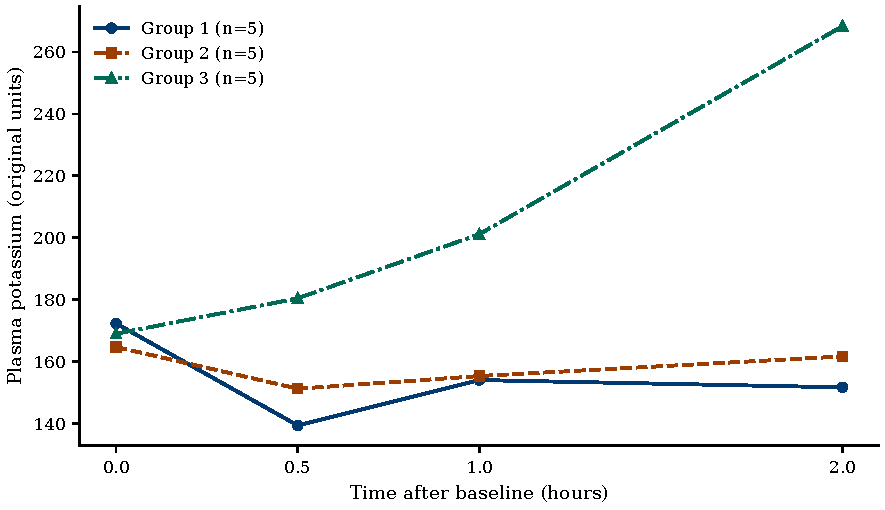
\includegraphics[width=.9\linewidth]{assets/rabbit_means.pdf}\end{center}

图为组均值，无置信区间；第3组后期明显上升，第1、2组相对平缓。交互有统计学证据，应优先描述不同时间过程，而非只给一个总体组差。

\textbf{SMA必须先定义指标。} 不等间隔下取基线校正曲线的时间平均变化 \[\Delta_i=\frac{1}{2}\int_0^2\{Y_i(t)-Y_i(0)\}\,dt,\] 积分以梯形法估计。第1、2组均值为−20.2500、−7.6475；Welch t=−1.3001，df\(\approx\) 7.999，P=.2298，差值95\% CI为(−34.956, 9.751)，证据不足。若按3个处理后时点直接平均再减基线，两组为−23.9533、−8.6333，P=.2025；若用个体线性斜率，P=.4758。原题``平均变化量''未唯一规定算法，应说明所采用的SMA定义，不能混淆变化量与变化率。


\Answer{C21-4}{Attention Blink的重复测量分析}

还原依据：正文的134人资料中删去原组2（23名乒乓球选手），剩余111行的8个观测值与2023附件逐值一致；保留原组1、3、4后重标为1、2、3，各均数与回忆稿完全相符。原附件未改写，还原CSV单独提供。

Mauchly \(W=0.074145\)，\(P\approx1.04\times10^{-42}\)，不满足球形性。GG系数0.514766，HF系数0.534728。以III型平方和为明确约定：

\begin{center}\small\setlength{\tabcolsep}{3.5pt}\renewcommand{\arraystretch}{1.18}\begin{tabular}{@{}lrrrrr@{}}
\toprule
效应 & F & 原df1 & 原df2 & 原P & GG校正P \\
\midrule

组别 & 1.57722 & 2 & 108 & 0.21127 & 不适用 \\
位置 & 42.38643 & 7 & 756 & \textless.001 & 2.84e-27 \\
组×位置 & 0.75126 & 14 & 756 & 0.72266 & 0.63241 \\
\bottomrule\end{tabular}\end{center}

位置校正自由度为约(3.6034, 389.1630)，交互为(7.2067, 389.1630)。原代码aov的顺序平方和与III型在不平衡组数下可检验不同加权主效应；本包同时保留aov输出，比较时不要混用。

\begin{center}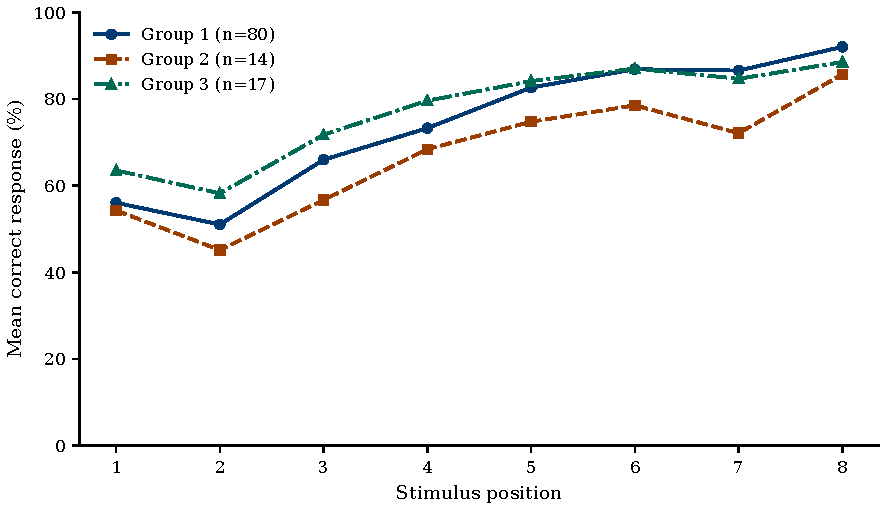
\includegraphics[width=.9\linewidth]{assets/attention_means.pdf}\end{center}

图只显示各组算术均值。p1---p8是刺激位置，原题没有给出足够信息换算成绝对时间。存在明显的位置变化，但组别及组×位置没有统计学证据；``不显著''不等于证明各组等效。

\clearpage\subsection*{补充练习解析}

以下为补充练习的解析。这些题目为配合正文新编，并非往年试题；题中设定的数值仅供练习。

\Answer{X26-4-1}{区组与条件重复的识别}

\textbf{答案：D。}

II是在同一人不同条件下重复测量，III是在同一人不同时点重复测量。I是区组内不同患者接受处理，每个人只提供一次结局；``有三种处理''不等于``同一人测三次''。是否重复须追溯实验单位，而不是只看资料按几列排列。




\Answer{X26-4-2}{协方差结构的判别}

\textbf{答案：C。}

三个差值方差分别为 \(4+6-2\times1=8\)、\(4+8-2\times2=8\)、\(6+8-2\times3=8\)，故II成立，也满足球形性对比条件。其对角元素不等、非对角元素也不等，不是CS结构。

若C的行是单位正交对比，\(C\mathbf1=0\)、\(CC^T=I_2\)，可验证 \(C\Sigma C^T=4I_2\)，所以III成立。本题区分原矩阵 \(\sigma^2I\)、CS与对比空间的广义球形性，不能把CS当作后者的必要条件。




\Answer{X26-4-3}{由对比协方差计算GG系数}

\textbf{答案：E。}

共有 \(4-1=3\) 个对比维度，故 \[\hat\varepsilon=\frac{(1+1+4)^2}{(4-1)(1^2+1^2+4^2)}=\frac{36}{54}=\frac23.\] 不能把分母中的``时点数减1''误写成4。应使用对比协方差阵的特征值；算出校正系数本身也不等于已完成球形性检验。




\Answer{X26-4-4}{多组资料为什么用合并残差协方差}

全部原始观测的协方差阵可能混入不同组均值轨迹之间的变异。正文的做法是先在各组、各时点减去相应组均数，计算组内协方差，再按组内自由度合并。若各组的理论协方差阵可视为共同的 \(\Sigma\)，则 \[S_{\mathrm{pool}}=\frac{\sum_{g=1}^{3}(n_g-1)S_g}{N-3},\qquad N=n_1+n_2+n_3.\] 等组数时它等于三个组内协方差阵的平均；组数不等时不能机械地等权平均。

令C为 \(4\times5\) 的单位正交对比矩阵，检验 \(CS_{\mathrm{pool}}C^T\) 对应的理论 \(4\times4\) 对比协方差阵是否与单位阵成比例。不能只对未经对比变换的 \(5\times5\) 原始矩阵检验 \(\Sigma=\sigma^2I\)，就把其拒绝结果解释为不满足H-F条件。




\Answer{X26-4-5}{麻醉诱导的重复测量输出填空}

\textbf{（1）设计与前提。} 组别是组间因素，时间是组内因素，独立受试者数为15而不是75。\(P=0.1776608<0.20\)，按题设拒绝H-F条件，对涉及时间的单变量检验采用GG校正。

\textbf{（2）未校正方差分析。}

\begin{center}\small\setlength{\tabcolsep}{5pt}\renewcommand{\arraystretch}{1.18}\begin{tabular}{@{}lllll@{}}
\toprule
来源 & SS & df & MS & F \\
\midrule

组别 & 912.2400 & 2 & 456.1200 & 5.7829 \\
个体间误差 & 946.4800 & 12 & 78.8733 & --- \\
时间 & 2336.4533 & 4 & 584.1133 & 106.5576 \\
组别×时间 & 837.6267 & 8 & 104.7033 & 19.1006 \\
个体内误差 & 263.1200 & 48 & 5.4817 & --- \\
\bottomrule\end{tabular}\end{center}

自由度相加为74。组别使用个体间误差作分母；时间与交互使用个体内误差作分母，不能混用。

\textbf{（3）校正后的读表结果。}

\begin{center}\small\setlength{\tabcolsep}{5pt}\renewcommand{\arraystretch}{1.18}\begin{tabular}{@{}lllll@{}}
\toprule
效应 & F（不变） & df1 & df2 & P \\
\midrule

组别 & 5.7829 & 2 & 12 & 0.01743 \\
时间（GG） & 106.5576 & 2.7148 & 32.5773 & \(1.87\times10^{-16}\) \\
组别×时间（GG） & 19.1006 & 5.4295 & 32.5773 & \(4.26\times10^{-9}\) \\
\bottomrule\end{tabular}\end{center}

时间的自由度为 \((4\varepsilon,48\varepsilon)\)，交互为 \((8\varepsilon,48\varepsilon)\)；组别检验不作该项校正。三个效应在0.05水平均显著。

\textbf{（4）过程解释。}

\begin{center}\small\setlength{\tabcolsep}{5pt}\renewcommand{\arraystretch}{1.18}\begin{tabular}{@{}llllll@{}}
\toprule
组别 & T0 & T1 & T2 & T3 & T4 \\
\midrule

A & 121.0 & 112.4 & 118.4 & 125.8 & 120.8 \\
B & 121.2 & 119.8 & 118.0 & 128.2 & 135.2 \\
C & 126.2 & 123.0 & 118.6 & 142.6 & 130.6 \\
\bottomrule\end{tabular}\end{center}

三组的平均时间轨迹不同：A组先降后回升，B组后期上升，C组在T3达到本组均数最高值后回落。交互显著说明组间差异随时间变化，不能用一个恒定组差概括，更不能从整体显著直接断言所有时点的任意两组均不同。

若前提水平改为0.05，则 \(P>0.05\)，不拒绝H-F条件；仅依据该检验，不再要求作GG校正，但这不等于证明总体严格满足球形性。

\textbf{两种输出的口径。} 本题据原始15行数据复算，与正文的软件输出一致。另一份汇总表的部分F值有舍入差异，且``校正''自由度采用更保守的下界 \(\varepsilon=1/4\)（不是本题给定GG系数）；两套自由度不能混填。
\EndExercises

\chapter*{附录\quad 易错表述与更正}
\addcontentsline{toc}{chapter}{附录\texorpdfstring{\quad}{ }易错表述与更正}
\markboth{附录\quad 易错表述与更正}{}
下表汇总学习中容易出现的不准确写法、记号或数据转录错误，并给出本书采用的写法，便于复习时对照。“位置”为本书的节号。
{\small\renewcommand{\arraystretch}{1.3}\setlength{\tabcolsep}{4pt}
\begin{longtable}{>{\raggedright\arraybackslash}p{1.5cm}>{\raggedright\arraybackslash}p{4.6cm}>{\raggedright\arraybackslash}p{4.6cm}>{\raggedright\arraybackslash}p{3.6cm}}
\toprule 位置&易错写法或表述&本书采用&说明\\\midrule\endfirsthead
\toprule 位置&易错写法或表述&本书采用&说明\\\midrule\endhead
\bottomrule\endfoot
1.1.5&迹“表示数据包含的总信息量”&各分量方差之和&受量纲影响\\
1.1.5&相关矩阵为单位阵“说明$p$个指标间相互独立”&两两不相关&联合正态时才等价于独立\\
1.2.2&$AB\ne BA$，“除非$B$为单位矩阵”&一般不可交换，$B=I$只是特例&如$B=cI$、$A^{-1}$\\
全文&转置记为$X'$或$X^T$&$X^\top$&$b_i'$另作他用，避免混淆\\
2.2.2&最大似然法“假设残差$e\sim N(0,\sigma^2)$”&误差$\varepsilon\sim N(0,\sigma^2I)$&残差不独立、不同方差\\
2.2.4&残差向量$E$、系数向量$B$；“各残差之和为0”&$e$、$b$；含截距时$\sum e_i=0$&避免与期望$E(\cdot)$混淆\\
2.3.2&“若模型假设成立且$H_0$成立，$b$服从$N(\beta,\sigma^2(X'X)^{-1})$”&正态模型下该分布不以$H_0$为前提&$H_0$只用于代入$\beta_i=0$\\
2.4&标准化系数记为$b_i'$；“体重对肺活量的作用比身高大”&记为$\widetilde b_i$；按标准差换算的条件关联&不直接代表重要性或因果\\
2.5&$C_p$：“应选择$C_p$最接近$p$的模型”&在$C_p\lesssim p$的模型中兼顾简洁性&全模型$C_p\equiv p$\\
3.1&$\mathrm{SRE}=e/\bigl(s\sqrt{1-h_{ii}^2}\bigr)$&$\mathrm{SRE}=e_i/\bigl(s\sqrt{1-h_{ii}}\bigr)$&与学生化残差的定义一致，$\Var(e_i)=\sigma^2(1-h_{ii})$\\
3.1&$e_t=\rho e_{t-1}+\varepsilon_t$，$-1\le\rho\le1$&$\varepsilon_t=\rho\varepsilon_{t-1}+u_t$，$|\rho|<1$&自相关是误差的性质\\
3.1&线性关系“不涉及检验，只作图”&以图为主，必要时检验&如加入二次项\\
3.1.1&\code{e1 <- lm(x3~x2+x4)}；\code{plot(e1,e2)}&\code{e1 <- resid(lm(...))}&应对残差作图\\
3.1.3&DW判断表只列三个区间&补入两个“不能确定”区&与DW分布图一致\\
3.2&“$(X'X)^{-1}$无解”&$X^\top X$奇异，系数不唯一，拟合值唯一&\\
3.3&岭回归“相对削弱自变量间的相关性”&改善$X^\top X$的病态&数据相关性不变\\
3.3&“寻找符号转正、岭迹平稳且较小的$k$值”&交叉验证/GCV选$k$，岭迹作参考&按预期符号选参不客观\\
3.4&$D_i=\dfrac{e_i^2}{(p+1)\widehat\sigma^2}\dfrac{h_{ii}}{(1-h_{ii})^2}$（$p$为自变量个数）&$D_i=\dfrac{e_i^2}{p\,s^2}\dfrac{h_{ii}}{(1-h_{ii})^2}$（$p$含截距）&记号不同，数值相同\\
4.1&“线性回归更专注于连续变量的预测”&线性回归同样可含分类自变量与交互&与广义线性模型区分\\
4.2.1&“此模型只能手算”；参数写作$\beta=(5.436,2.781,3.956)$&软件可处理秩亏模型；写作估计值$\widehat\beta$&\\
4.3&“两步随机”；“全组哑变量模型无法用软件实现”&区组既有，组内一步随机化&\\
4.4.1&交互作用图中$b=1$线为$(1,2.1)$--$(2,1.2)$，$b=2$线为$(1,1.0)$--$(2,0.8)$&$b=1$：$(1,2.1)$--$(2,1.0)$；$b=2$：$(1,1.2)$--$(2,0.8)$&与格子均数表一致\\
4.4.2&$\widehat\alpha_1=1.7-1.3=0.4$，$\widehat\beta_1=1.6-1.3=0.3$等（按1.3代入），交互效应式中亦代入1.3&统一用总均数1.275：$\pm0.375$、$\pm0.275$、$\pm0.175$&按1.3代入时交互式应得0.2，与0.175不一致\\
4.4.3&$SS_A=\sum(\bar Y_i-\bar Y)^2$等，误差自由度$ab(n-1)$&$SS_A=br\sum_i(\cdot)^2$，$SS_B=ar\sum_j(\cdot)^2$，$SS_{AB}=r\sum\sum(\cdot)^2$；$ab(r-1)$&补齐权重\\
4.4.3&$H_0$：交互作用无统计学意义&$H_0:(\alpha\beta)_{ij}=0$&假设针对总体参数\\
4.5&“消除混杂因素的影响”&对已测协变量作线性调整&\\
4.5.1&“饱和模型”；“$P>0.05$，应用简略模型/平行”&含交互项的完整模型；未发现斜率差异的证据&\\
4.5.4&“若要与进入顺序无关，应选三型平方和”&先明确假设，再选平方和类型&\\
5.1.2&“$t_0-t_1,t_0-t_2,\ldots$这样比较是错的”&可配对比较，按预设范围控制多重性&\\
5.3.2&第二个复合对称矩阵非对角元为$\sigma_1$&$\sigma_1^2$&\\
5.3.3&$\sigma_{ij}=\frac{\sigma_{ii}+\sigma_{jj}}2-\lambda\ \longrightarrow\ \lambda=\sigma_{ii}+\sigma_{jj}-2\sigma_{ij}$&$\Var(Y_i-Y_j)=\sigma_{ii}+\sigma_{jj}-2\sigma_{ij}=2\lambda$&右侧应为$2\lambda$\\
5.3.3&HF结构“存在正交变换矩阵$C$，使$C^T\Sigma C$满足球形假设”&$C^\top\Sigma C=\lambda I_{k-1}$，$C^\top C=I$，$C^\top\mathbf 1=0$&对任意此类$C$成立\\
5.4.1&$\chi^2=-\Bigl[(n-1)-\dfrac{n-(2p^2+2)}{6p}\Bigr]\ln\lambda$，$\nu=\dfrac{p(p-1)}2-1$&$-\Bigl[\nu-\dfrac{2d^2+d+2}{6d}\Bigr]\ln W$，自由度$\dfrac{d(d+1)}2-1$&与正文R程序一致\\
5.4.4&$\varepsilon=\dfrac{(\sum_{i=1}^k\lambda_i)^2}{(k-1)\sum_{i=1}^k\lambda_i^2}=\dfrac{[\tr(S)]^2}{(k-1)\tr(S^2)}$；“对$F$值校正”&用$A=C^\top SC$的$k-1$个特征值；$F$不变，校正自由度&应对$C^\top SC$计算\\
5.5&$F_{\text{时间}}=\dfrac{\SSq{时间}/(p-1)}{\ms{误差}/[(n-1)(p-1)]}$&分母为$\SSq{误差}/[(n-1)(k-1)]$&避免两次除以自由度\\
5.6.4&$C^\top SC$第3行第3列为$11.9966667$&$1.9966667$&与$W$、GG系数一致\\
5.6.5&表12-20“自由度（校正）”$1,2,12$未注明方法&下界校正$\varepsilon=1/4$&非GG校正\\
5.6.5&记号$g$（组数）、$m$（次数）&$a$、$k$&与第5章统一\\
\end{longtable}}

\end{document}
